
\documentclass[final]{ntnuthesis}

\usepackage{wdefault}
\newcommand{\myfigwidtha}{0.7\textwidth}

%\def\abstract{\section{Abstract}}
%\def\endabstract{}
%\usepackage{IEEEtrantools}
\newtheorem{exmp}{Example}[section]

\newcommand{\CWabstract}[1]{
\section{#1}
}
\newtheorem{IEEEproof}{Proof}

\setcounter{lofdepth}{2}
\usepackage{setspace}
\onehalfspacing

%-------------------------------------------------------
% Title
%-------------------------------------------------------
\bibliographystyle{IEEEtran}
\title{Efficient ADCs for nano-scale CMOS Technology}
\author{Carsten Wulff}
\degreetype{PhD}
\faculty{Faculty of Information Technology, Mathematics and Electrical Engineering}
\department{Department of Electronics and Telecommunications}
\setmonth{December}
\setyear{2008}
\issnprinted{N/A}
\isbnprinted{978-82-471-1286-1}
\isbnelectronic{978-82-471-1287-8}
\renewcommand{\bibname}{References}
\renewcommand{\figurename}{Fig.}
\renewcommand{\myfignamehead}{Fig.}

%2008:292  	ISBN 978-82-471-1287-8  	Electronic  	2008-10-22
%2008:292 	ISBN 978-82-471-1286-1 	Printed 	2008-10-22

\begin{document}
\pagenumbering{arabic}
\maketitle

\chapter*{Abstract}\addcontentsline{toc}{chapter}{Abstract}
The topic of this thesis is efficiency of analog-to-digital
converters (ADC) in nano-scale CMOS technology. With  downscaling of CMOS
technology it is  harder to design ADCs. The power supply is reduced due to reliability concerns and the output resistance of
transistors is reduced because of shorter channel lengths. Such
challenges makes it harder to design ADCs with conventional circuit
techniques and ADC architectures.

We investigate two separate paths towards higher efficiency
in nano-scale CMOS technologies: circuit implementation, and ADC architectures. 

The research into ADC architectures assumes that circuit
implementation challenges will be solved. It looks at how a sigma-delta modulator can
be used as a front-end to pipelined ADCs. A new class of sigma-delta
modulators, the switched-capacitor (SC) open-loop sigma-delta
modulator (OLSDM) is introduced. We introduce the SC modulo integrator
and the SC modulo resonator that facilitates implementation of
sigma-delta modulators that do not have feedback of the quantized
signal. Thus, high-latency converters such as pipelined ADCs can be
used as quantizers. Limitations of OLSDM, like operational amplifier (opamp) DC gain,  quantizer
linearity, and input signal amplitude are discussed in
detail. Behavioral simulations of OLSDMs confirm the theory. 


The research into circuit implementations investigate how the opamp can be
removed from SC circuits. Two techniques are
investigated: open-loop residue amplification and comparator-based
switched-capacitor circuits (CBSC). 

 We
present the design of a 7-bit 200MS/s 2mW pipelined ADC based on
switched open-loop residue amplifiers.  By turning off the open-loop
amplifiers when they are not needed the  power
dissipation is reduced by 23\%. 

Comparator-based switched-capacitor circuits (CBSC) are an alternative
to opamp based SC circuits. By replacing the opamp
with a comparator and current sources the same charge transfer is
achieved. 

We discuss design equations for CBSC, and how one can model CBSC in
MATLAB and SPICE.

We present an 8-bit 60MS/s 8.5mW pipelined ADC with 7.05-bit effective
number of bits (ENOB). At the time of writing
it was the first silicon
proven differential CBSC pipelined ADC. 



%%%%%%%%%%%%%%%%%%%%%%%%%%%%%%%%%%%%%%%%%%%%%%%%%%%%%%%%%%%%%%%%%%%%%%%
%% Ferrata.tex
%% Description:   
%% Author:        Carsten Wulff <wulff@iet.ntnu.no>
%% Created at:    Fri Oct 10 19:32:25 2008
%% Modified at:   Fri Oct 10 19:42:10 2008
%% Modified by:   Carsten Wulff <wulff@iet.ntnu.no>
%%%%%%%%%%%%%%%%%%%%%%%%%%%%%%%%%%%%%%%%%%%%%%%%%%%%%%%%%%%%%%%%%%%%%%
\chapter*{Errata}\addcontentsline{toc}{chapter}{Errata}
I wanted this document, this almost 200 page document, to be free of
errors. But I should know better by now. This is a list of the errors
I could find before submitting this thesis for printing, there are
probably some I did not find, for which I appologize. The errors were
not corrected since the papers should be an exact copy of the papers
published in the literature. 

\section*{Paper 3}
\begin{enumerate}
\item Section 6.5.2, Last sentence: Fig. 6.19 $->$ Fig 6.18
\item Section 6.5.3, Second paragraph: Fig 6.20 $->$ Fig. 6.21
\end{enumerate} 

%%%%%%%%%%%%%%%%%%%%%%%%%%%%%%%%%%%%%%%%%%%%%%%%%%%%%%%%%%%%%%%%%%%%%%
%% Fpreface.tex
%% Description:   
%% Author:        Carsten Wulff <wulff@iet.ntnu.no>
%% Created at:    Thu Apr 24 16:35:47 2008
%% Modified at:   Mon Nov  3 17:18:51 2008
%% Modified by:   Carsten Wulff <wulff@iet.ntnu.no>
%%%%%%%%%%%%%%%%%%%%%%%%%%%%%%%%%%%%%%%%%%%%%%%%%%%%%%%%%%%%%%%%%%%%%%

\chapter*{Preface}\addcontentsline{toc}{chapter}{Preface}
This thesis was submitted to the Norwegian University of Science and Technology 
(NTNU) in partial fulfilment of the requirements for the degree of philosophiae 
doctor (PhD). 
The work presented herein was conducted at the Department Electronics
and Telecommunication, NTNU, under the supervision of Professor Trond
Ytterdal, with Professor Trond S{\ae}ther as co-advisor. Financial support from the Norwegian Research Council through the
project Smart Microsystems for Diagnostic Imaging in Medicine (project
number 159559/130) and the project ASICs for Microsystems (project
number 133952/420) is gratefully acknowledged.


\section*{Research Path}
This is a document that has been four years in the making. I began by
my  work in January 2004. The intent was to investigate calibration
algorithms for micro-systems, with focus on genetic algorithms. But I
strayed from this path and found analog-to-digital converters. The project
Smart Microsystems for Diagnostic Imaging in Medicine (SMIDA) needed a
low resolution high speed ADC, and I was asked to build it. This led to some initial work on dynamic comparators, opamps in
90nm CMOS and bootstrapped switches. 

Wislands doctoral thesis (2003) on \textit{Non-feedback Delta-Sigma
  modulators for digital-to-analog conversion} peaked my
interest. We\footnote{ Trond Ytterdal and I}
wanted to see if we could apply the open-loop sigma-delta technique to
analog-to-digital converters. We believed they could be used as
front-ends to pipelined ADCs. In that respect, we developed techniques
for switched-capacitor circuits. 

At ISSCC 2006 the first comparator-based switched-capacitor circuit
was published, and we immediately jumped on it. From the summer of 2006
to the summer of 2007 my time was dedicated to tape-out the first
differential comparator-based switched-capacitor ADC. That year
I was fortunate to spend my time at the
University of Toronto as a visiting researcher.  The time in Toronto inspired much
of my work, like the open-loop residue amplifiers for pipelined ADC,
and the continuous time bootstrapped switches. 

My chip came back in January 2008, and most of the spring was spent on
making the chip work. On the first day I
got 4.2-bit ENOB, and it took me four months to get to 7.05-bit.

As these four and a half years draw to a close, I find that I am
satisfied. In a sense I have come full circle with the genetic
algorithm used to calibrate my ADC. 


\section*{Acknowledgements}
\begin{itemize}
\item To my wife, Anita, without her this thesis
would not have seen the light of day. She was willing to move half way
around the world with me, for which I am forever grateful. 
\item To my son, Villem, born during my years as a PhD student you have shown me that
  it's possible to get up at 05:30 {\sc a.m} and still
  survive the day. This has been immensely helpful. Your smiles and hugs
  brighten my mood after a long day at work.
\item To my late mother, my dad, my sisters and my extended family for
  your love and support.
\item To my supervisor, Trond Ytterdal, he has always been available
  for questions and his guidance is valued. He has provided the resources necessary to do this
  work.  
\item To my co-advisor, Trond S{\ae}ther, for his support and
  convincing me that analog integrated circuits was the way to go.
\item To my colleagues at Department of Electronics and
  Telecommunication, Circuits and Systems Group for lunch discussions,
  coffee sessions and support.
\item To my fellow PhD students for many
  fun discussions: {\O}ystein
  Gjermundnes, Ashgar Havashki, Are Hellandsvik, Tajeshwar Singh, Ivar
  L{\o}kken, Anders Vinje, Saeeid Tahmasbi Oskuii,
   Linga Reddy Chenkeramaddi and Bertil Nistad. 
\item To Johnny Bj{\o}rnsen for help with measurements.
\item To my fellow graduate students during my stay in Toronto for
  their hints and tips: Imran Ahmed, Bert Leesti, Ahmed Gharbiya,
  Trevor Caldwell and Pradip Thachile.
\item  A special thanks to Professors
  Ken Martin and David Johns for many useful questions and
  suggestions.  
\end{itemize}

\section*{Comments on style}
In a break from conventional page numbering this thesis start with
page number 1 on the title page. In this digital age it is likely that this
thesis will be read on a computer. As the title page is page one, the
page numbers of the thesis will match the page numbers of the electronic
document. I believe this will make the thesis easier to navigate.



\cleardoublepage
\addcontentsline{toc}{chapter}{Table of contents}
\tableofcontents
\cleardoublepage
\addcontentsline{toc}{chapter}{List of figures}
\listoffigures
\cleardoublepage
\addcontentsline{toc}{chapter}{List of tables}
\listoftables


\chapter*{List of abbreviations} \addcontentsline{toc}{chapter}{List
of abbreviations}
%\begin{table}[h]
%\centering
%\renewcommand{\arraystretch}{1.3}
\begin{tabular}{l l}
ADC & Analog-to-digital converter\\
ADSL & Asymmetric digital subscriber line\\
ASIC & Application specific integrated circuit\\
%BFS &\\
CBSC & Comparator-based switched-capacitor\\
CMOS & Complementary metal oxide semiconductor\\
DAC & Digital-to-analog converter\\
DC & Direct current\\
DITS & Drain-induced threshold shift\\
DIBL & Drain-induced barrier lowering\\
DNL & Differential non-linearity\\
DRAM & Dynamic random access memory\\
%ECG & Electrocardiogram\\
ENOB & Effective number of bits\\
ERBW & Effective resolution bandwidth\\
FFT & Fast Fourier transform\\
FOM & Figure of merit\\
%ICEE & International\\
IC & Integrated Circuit\\
IEEE & Institute of Electrical and Electronics Engineers\\
INL & Integral non-linearity\\
IO & Input - Output \\
ISSN & International Standard Serial Number\\
ITRS & International Technology Road-map for Semiconductors\\
JSSC & Journal of solid state circuits\\
GPRS &General Packet Radio Service\\
LDI & Lossless discrete integrator\\
LSB & Least significant bit\\


\end{tabular} 

\begin{tabular}{l l}
LC-SDM & Low-pass Conventional Sigma-Delta Modulator\\
L-SDM & Low-pass  Sigma-Delta Modulator\\
MASH & Multi-stAge noise SHaping\\
MDAC & Multiplying digital-to-analog converter\\
MOSFET & Metal oxide semiconductor field effect transistor\\
MSB & Most significant bit\\
NMOS & n-channel MOSFET\\
NTF & Noise transfer function\\
NTNU & Norwegian university of science and technology\\
NUD & Number of unit devices in parallel\\
OLSDM & Open-loop sigma-delta modulator or open-loop sigma-delta modulation \\
opamp & Operational amplifier\\
OSR & Oversampling ratio\\
%OTA & Operational transconductance amplifier\\
PMOS & p-channel MOSFET\\
PSD & Power spectral density\\
RMS & Root mean square\\
%SACD & Super audio CD\\
SADC & Sub analog-to-digital converter\\
SAR & Successive approximation register\\
SC & Switched-capacitor\\
SDM & Sigma-delta modulation\\
SFDR & Spurious free dynamic range\\
SMIDA & Smart Microsystems for Diagnostic Imaging in Medicine \\
SNDR & Signal to noise and distortion ratio\\
SNR & Signal to noise ratio\\
SoC & System-on-Chip\\
SPICE & Simulation Program With Integrated Circuit Emphasis\\
\end{tabular} 

%\end{table}


%%%%%%%%%%%%%%%%%%%%%%%%%%%%%%%%%%%%%%%%%%%%%%%%%%%%%%%%%%%%%%%%%%%%%%
%% Fpapers-intro.tex
%% Description:   
%% Author:        Carsten Wulff <wulff@iet.ntnu.no>
%% Created at:    Mon May 26 12:39:52 2008
%% Modified at:   Wed Oct 29 15:27:03 2008
%% Modified by:   Carsten Wulff <wulff@iet.ntnu.no>
%%%%%%%%%%%%%%%%%%%%%%%%%%%%%%%%%%%%%%%%%%%%%%%%%%%%%%%%%%%%%%%%%%%%%%


\chapter*{List of appended papers}\addcontentsline{toc}{chapter}{List of appended papers}

\paragraph{1.}\textbf{Analog Modulo Integrator For Use In Open-Loop Sigma-Delta
  Modulators}\\
\indent Carsten Wulff, {\O}ystein Knauserud, Trond Ytterdal\\
\indent In proceedings of the 24th NORCHIP Conference, 2006.\\
\indent Nov. 2006 Pages 125 - 128\\
\indent Digital Object Identifier 10.1109/NORCHP.2006.329259 \\

\paragraph{2.}\textbf{Switched capacitor analog modulo integrator for application
  in open loop sigma-delta modulators}\\
\indent Carsten Wulff, {\O}ystein Knauserud, Trond Ytterdal\\
\indent Analog Integrated Circuits and Signal Processing\\
\indent Springer Netherlands, ISSN 0925-1030\\
\indent Volume 54, Number 2, Pages 121-131 February 2008\\
\indent DOI 10.1007/s10470-007-9084-2\\

\paragraph{3.}\textbf{Resonators in open-loop sigma-delta modulators}\\
\indent Carsten Wulff and Trond Ytterdal\\
\indent Submitted to IEEE Transactions on Circuits and Systems I: Regular Papers\\

\newpage
\paragraph{4.}\textbf{ 0.8V 1GHz Dynamic Comparator in Digital 90nm CMOS
  Technology}
\newline
\indent   Carsten Wulff and Trond Ytterdal\\
\indent In proceedings of the 23rd NORCHIP Conference, 2005. \\
\indent 21-22 Nov. 2005 Pages 237 - 240 \\
\indent Digital Object Identifier: 10.1109/NORCHP.2005.1597033\\

\paragraph{5.}\textbf{Design of a 7-bit 200MS/s, 2mW Pipelined ADC With Switched
  Open-Loop Amplifiers In a 65nm CMOS Technology}\\
\indent Carsten Wulff and Trond Ytterdal\\
\indent In proceedings of the 25th NORCHIP Conference, 2007.\\
\indent  Digital Object Identifier 10.1109/NORCHP.2007.4481042 \\


\paragraph{6.}\textbf{Design and Behavioral Simulation of Comparator-Based Switched
  Capacitor Circuits}\\
\indent Carsten Wulff and Trond Ytterdal\\
\indent Accepted at NORCHIP 2008\\

\paragraph{7.}\textbf{An 8-bit 60-MS/s 8.5mW Differential Comparator-Based Switched-Capacitor
  Pipelined ADC in 90nm CMOS Technology}\\
\indent Carsten Wulff and Trond Ytterdal\\
\indent Submitted to IEEE Journal of Solid State Circuits\\

The following papers have also been published. Because they fall outside
the  theme of this thesis they are not included in the thesis.\\

\paragraph{A }\textbf{Next Generation Lab - A Solution for remote
  characterization of analog integrated circuits}\\
\indent Carsten Wulff, Trond Ytterdal, Thomas Aas Saethre, Arne Skjevlan,
Tor A. Fjeldly and Michael S. Shur\\
\indent Fourth IEEE International Caracas Conference on Devices, Circuits and
Systems, Aruba, April 17-19, 2002.\\


\paragraph{B}\textbf{Programmable Analog Integrated Circuit for use in remotely
  operated laboratories}\\
\indent Carsten Wulff and Trond Ytterdal\\
\indent International Conference on Engineering Education, ICEE-2002\\
\indent August 18-21, 2002, Manchester, U.K.\\
%\newpage
\paragraph{C}\textbf{Programmable Analog Integrated Circuit}\\
\indent Carsten Wulff, Roger Erstad and Trond Ytterdal\\
\indent In Proceedings of the 22nd NORCHIP Conference, 2004.\\
\indent Nov. 2002, Pages 99 - 102\\

\paragraph{D}\textbf{High Speed, High Gain OTA in a Digital 90nm CMOS
  Technology}\\
\indent {\O}yvind Berntsen, Carsten Wulff, Trond Ytterdal\\
\indent In proceedings of 23rd NORCHIP Conference, 2005.\\
\indent 21-22 Nov. 2005 

\paragraph{E}\textbf{Bootstrapped Switch In Low-Voltage Digital 90nm CMOS
  Technology}\\
\indent Christian Lillebrekke, Carsten Wulff and Trond Ytterdal\\
\indent In proceedings of 23rd NORCHIP Conference, 2005.\\
\indent 21-22 Nov. 2005 

\paragraph{F}\textbf{New Approach for Continuous Time Sigma Delta Modulators}\\
\indent Francisco Colodro, Marta Laguna, Carsten Wulff, Trond Ytterdal and
\indent Antonio Torralba\\
\indent In proceedings of 23rd NORCHIP Conference, 2005.\\
\indent 21-22 Nov. 2005 

%%% Local Variables: 
%%% mode: latex
%%% TeX-master: "thesis"
%%% End: 

%\pagestyle{headings}
%\pagenumbering{arabic}
%%%%%%%%%%%%%%%%%%%%%%%%%%%%%%%%%%%%%%%%%%%%%%%%%%%%%%%%%%%%%%%%%%%%%%
%% Fintroduction.tex
%% Description:   
%% Author:        Carsten Wulff <wulff@iet.ntnu.no>
%% Created at:    Thu Apr 24 16:32:35 2008
%% Modified at:   Wed Oct 29 19:44:58 2008
%% Modified by:   Carsten Wulff <wulff@iet.ntnu.no>
%%%%%%%%%%%%%%%%%%%%%%%%%%%%%%%%%%%%%%%%%%%%%%%%%%%%%%%%%%%%%%%%%%%%%%
\chapter{Introduction}\label{sc:intro}


How can we make efficient analog-to-digital converters (ADCs) in nano-scale
CMOS?
Challenges like reduced headroom and reduced output resistance has
made it hard to design efficient ADCs in the new nano-scale CMOS technologies.
Why do we want more efficient ADCs? The simple answer is: longer
battery life. The ADC is a key component in any signal chain that
interface with the real world. The receive chain of GPRS networks, Wi-Fi
networks, indeed any current mobile wireless communication technology has an
ADC. Most of the processing today is done in the digital
domain. The pure analog signal chains have been banished to obscurity. But the real world
is analog, and information from the real world must be converted to
digital before it can be digitally processed.

Consumers demand high speed mobile networking on 
the bus to work, at the local cafe, and in their homes. They want 
their portable devices
to have infinite battery lives, and they should cost nothing. 
To
reduce the cost and increase efficiency there has been a push for
integration of features on a single chip (System-on-Chip). 
In SoCs with high integration most of the functions are digital, thus
technologies that allow cheap integration of digital features are
used. These are the nano-scale technologies (less than 100nm
transistor gate length). 

%Two of the challenges that face an analog
%designer in nano-scale CMOS are: reduced headrom, and reduced output resistance.


%\n{Reduced headroom}
Reliability concerns of downscaled CMOS transistors has lead to a
decrease in power supply. At high electrical fields the transistor
gate oxide breaks down. In downscaled transistors the thickness of
the gate oxide is reduced, hence the maximum power supply  must be
reduced. Fig. \ref{fig:supplyscaling} shows the historic power supply  and
  future trends (from ITRS 2007 \cite{itrs07}). At the 250nm gate
  length the power supply is 2.5V, but in 90nm  the power supply
  is reduced to 1.2V.

A challenge with reduced power supply is the reduced signal swing, 
in most cases the signal swing cannot be larger than the power supply.
The accuracy of an ADC is proportional to sampling
capacitance\footnote{This is easily seen from the equation
\eqn{
  S/R = \frac{Signal\:Power}{Noise\:Power} = \frac{A^2/2}{kT/C} = \frac{A^2 C}{2kT}
}}, and
sampling capacitance is inversely proportional to the square of the
signal swing.
 Hence, the capacitor
  size quadruples when we go from 250nm to 90nm CMOS
  technology for the same accuracy. An increased
  capacitor size result in higher area consumption and increased cost.
\begin{figure}[htbp]
\centerline{ 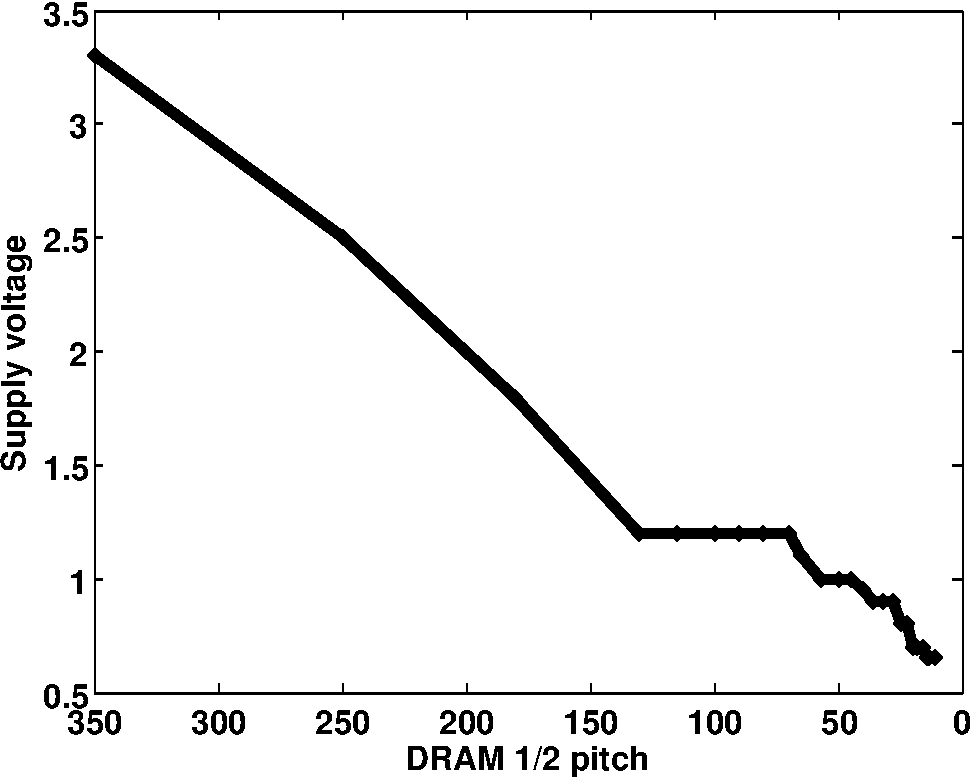
\includegraphics[width=\myfigwidthb]{graphics/supplyscaling}}
  \caption{Historic and future 
    scaling of power supply (based on ITRS 2007
    \cite{itrs07}). DRAM 1/2 pitch is smallest half-pitch of
  contacted metal lines in a DRAM cell.} 
  \label{fig:supplyscaling}
\end{figure}


%\subsection{Reduced output resistance} 
Another challenge is the reduced output resistance of nano-scale CMOS transistors.
  As devices are scaled down the
  transistor channel lengths  shorten. At shorter channel lengths channel
  length modulation and drain induced barrier lowering \cite{troutman79} reduce the output resistance of the
  transistor. Longer channels can be used to increase
  the output resistance, but the effectiveness of using a longer channel is reduced by the pocket
  implants \cite{cao99}. Pocket implants are used to reduce $V_T$ roll-off and
  punch-through in nano-scale technologies. 
%At longer channel lengths the pocket
%  implants cause a drain induced threshold shift (DITS).
% The impact of
%  the pocket implants depend on their dosing concentration, a higher
%  dose lead to a lower output resistance.  
Due to the pocket implants the output resistance of a 1$\mu$m long
  transistor in a 90nm technology is lower than a 1$\mu$m long transistor in
  a 350nm technology.

For high accuracy circuits we need high gain in our transistors. The
gain in a transistor is proportional to the output resistance of the
transistor. The gain of the single transistor is called the intrinsic
gain. 
%The output resistance influence the intrinsic gain of a transistor.
%Longer channels can be used to increase output
%  resistance, but the drain-induced
%  threshold shift (DITS) caused by the pocket implant used in
%  nano-scale technologies 
%  The 
%  intrinsic gain is a measure of how much gain we can
%  expect from one transistor. 
It is
  defined as $A_i =  g_m/g_{ds}$, where $g_m$ is the transconductance
  and $g_{ds}$ is the output conductance (inverse of output
  resistance). 
  When the output resistance is reduced the intrinsic gain
  goes down, and in 65nm technology the intrinsic gain of a minimum
  device is 6\footnote{$L=0.06$, $W=10L$, $V_{DS}=V_{DD}/2$,
    $V_{EFF} = V_{DD}/8$, typical corner} (15-dB). In 350nm technology a minimum 
  device has a gain of 43\footnote{$L=0.35$, $W=10L$, $V_{DS}
    = V_{DD}/2$, $V_{EFF} = V_{DD}/8$, typical corner} (32-dB). As a result, one must use multiple
  stages, cascoding, or gain boosting to achieve high gain amplifiers
 in 65nm technology. But techniques like cascoding (stacking
 transistors) is hard in 65nm technology due to the low supply
 voltage. 
%\end{description}

Downscaling of analog circuits is not all bad. The speed can be
increased due to shorter channel lengths, and the parasitic
capacitances are smaller. But these two advantages are overshadowed by
the reduction in gain and power supply.


We believe that efficiency in nano-scale technology is best attacked
from both ends: the circuit implementation, and the ADC architecture.


One approach to efficiency is to investigate the architectural level. If we
assume that the circuit challenges can be solved, can we do anything
about the ADC architectures? High
accuracy (14-bit) high-speed ($>$ 10MS/s) ADCs are challenging to
implement in nano-scale technologies because of the large sampling
capacitors. With a 1V input
signal swing the
sampling capacitors will be 53pF for a 14-bit converter, which is a
large capacitor. To reduce the sampling capacitor we can use
oversampling. In sigma-delta modulators oversampling is used in
addition to quantization noise shaping to achieve high
accuracy. We wanted to investigate a class of sigma-delta modulators
called \textit{Open-Loop Sigma-Delta Modulators} (OLSDM), and their
use as a front-end to pipelined ADCs. The part of this thesis that
focus on OLSDM is of a theoretical nature.

The other approach to increased efficiency is to investigate the
circuit implementation. 
Switched-capacitor (SC) circuits are ubiquitous in ADCs. They are a tried
and tested accurate method of implementing  high speed
ADCs. The sigma-delta modulators and pipelined ADCs predominate in
the use of SC circuits. The traditional approach to SC  circuits use
opamps, which consume most of the
power in an ADC. In nano-scale technology opamps have become
increasingly hard to design due to the reduced headroom and decreased
output resistance. Techniques that replace opamps have received
interest from the research community. Part of this thesis investigate
how one can replace opamps in pipelined ADCs, and through
this improve efficiency. This part of the thesis is a combination of
theoretical work and measurements on a nano-scale CMOS ADC. 


\section{Main contributions}
The main contributions of this thesis are:


%\subsection{Efficient architectures for pipelined ADCs}
\begin{itemize}
\item We introduce the switched-capacitor modulo integrator. It facilitates
  implementation of switched-capacitor open-loop sigma-delta
  modulators.
\item We introduce the switched-capacitor open-loop sigma-delta
  modulator. A versatile type of sigma-delta modulator suited as
  front-end to pipelined ADCs
\item We introduce the modulo resonator. It enables implementation of high
  resolution open-loop sigma-delta modulators with low oversampling ratio.
\item We prove that open-loop sigma-delta modulation is equivalent to
  sigma-delta modulation if
\eqn{
  |x_n| < R\left(\frac{1}{2} - \frac{2^{N-1}}{2^B}\right)
}
where $x_n$ is the input signal at time $n$, $R$ is the full scale
range, $N$ is the order of the modulator and $B$ is the number of bits in
the quantizer.
\item We introduce the switched open-loop residue amplifiers. Using these the power
  dissipation is reduced by 23\% for a  7-bit pipelined ADC.
\item We introduce the first fully differential silicon proven comparator-based
  switched-capacitor pipelined ADC. Differential implementation allow
  higher signal swing, which is essential
  in nano-scale technologies.

\end{itemize}
Other significant contributions are:

\begin{itemize}

\item We present a comprehensive figure of merit survey of ADCs in Journal of Solid State
  Circuits (1975-2008) and
  International Solid State Circuits conference (2000-2008).
\item We present the  limits of figure of merit for ADCs
\item We present design equations for comparator-based
  switched-capacitor circuits.
\item We introduce a simple calibration scheme for comparator threshold
  calibration. This technique cancels the overshoot in
  comparator-based switched-capacitor pipelined ADCs

\end{itemize}

%\end{enumerate}

%\subsection{Open-Loop Sigma-Delta Modulators}
%\begin{enumerate}




\section{Thesis outline}
This thesis is a collection of papers, hence the 
results are in the papers. The research presented in this thesis is on analog-to-digital
converters, with focus on pipelined ADCs and sigma-delta modulators. If this subject is unfamiliar we suggest reading 
Chapters 9, 10, 11, 13 and 14  in \cite{johns}. 
%For your convenience we have included an introduction
%to ADCs in 
%(Appendix \ref{ap:primer}) and  an introduction to the mathematics of noise sources
%(Appendix \ref{ap:noise}).


This thesis is organized as follows: Chapter \ref{sc:limits} discuss
the fundamental limits of ADC figure of merit, and how parasitic
capacitance make it hard to implement a low resolution converter with
high efficiency.

In Chapter \ref{sc:research} the papers are introduced and we detail how the papers are related. 
The papers are presented in Chapter \ref{sc:p1} to Chapter
\ref{sc:p7}. Comments to papers, a conclusion and further work is
presented in Chapter \ref{sc:remarks}

%In Chapter \ref{sc:papers} the papers are presented.


%%% Local Variables: 
%%% mode: latex
%%% TeX-master: "../../wulff/work/ntnu/phd/thesis/tb_introduction"
%%% End: 

\chapter{Limits of ADC figure of merit}\label{sc:limits}
Efficiency is one of the key measures of analog-to-digital
converters. A more efficient
ADC can translate into longer battery life of our
hand-held devices. For ADCs the power dissipation ($P$), sampling frequency
($f_s$) and effective number of bits ($B$) are combined to give a
single measure of the efficiency, the figure of merit (FOM). 
For the
figures of merit discussed here a smaller value is better. 

The
historic figure of merit proposed by Walden \cite{walden99}
was \req{fomwalden}\footnote{It was actually presented as $FOM =2^Bf_s/P$, but the
  inverse is the most used.}
  \begin{equation}
    \label{eq:fomwalden}
    FOM = \dfrac{P}{2^{B}f_s}
  \end{equation}
This FOM, however, is incorrect if we assume the ADCs should be limited by
thermal noise. A more correct figure of merit is
  \begin{equation}
    \label{eq:fom}
    FOM = \dfrac{P}{2^{2B}f_s}
  \end{equation}

This figure of merit, the Thermal FOM, is based on the fact that in an
ADC limited by thermal noise we must use 4 times the power if we add
one bit of resolution, since the required sampling capacitance increases 4 times. A more
in-depth argument is given in \cite{schreier.uds} on page 360. 

If we have the ADC parameters (accuracy, power dissipation, speed) we
can calculate the FOM from \req{fom}. But
what is the limit of the FOM? How low FOM can we expect to get with
future ADCs? 

We will in this chapter derive expressions for the FOM
limit and compare the limit to results of published ADCs. But first 
we have to derive the required sampling
capacitance for a certain resolution.


\section{Required sampling capacitance}
We assume a switched-capacitor based ADC. The input signal is sampled
across a sampling capacitor ($C$). And $C$ is the only capacitor in
the ADC. In such a system the thermal noise
power can be represented as
\begin{equation}
\label{eq:thermal}
\overline{V_{thermal}^2} = a_1\times k T/C  
\end{equation}
where $a_1$ is a constant greater than one, $k$ is Boltzmann's constant, $T$ is the temperature
in Kelvin and $C$ is the sampling capacitance.

 The thermal noise power should be less
than the quantization noise power, but not too small, because a 
small thermal noise power will cost in terms of power dissipation. 
We assume that the quantization noise power is four times the thermal noise power.
\begin{equation}
  \label{eq:lsbvsthermal}
  \overline{V_{LSB}^2} = 4\times\overline{V_{thermal}^2}
\end{equation}
where $\overline{V_{LSB}^2}$ is the quantization noise power, which can
be calculated as
\begin{equation}
\label{eq:lsb}
\overline{V_{LSB}^2} = V_{LSB}^2/12= V_{PP}^2/(2^{2B}\times
  12)
\end{equation}
where $V_{LSB}$ is the voltage step of the least significant bit (LSB)
and  $V_{PP}$ is the peak-to-peak
input signal voltage.

If we combine \req{thermal}, \req{lsbvsthermal} and \req{lsb} we get
\begin{equation} 
  \label{eq:cap1}
 \dfrac{ V_{PP}^2}{2^{2B}\times12} = 4 \times a_1 \times kT/C
\end{equation}

Solved for sampling capacitance ($C$) \req{cap1} becomes
\begin{equation}
\label{eq:cap}
C = a_1 \times \dfrac{48 k T 2^{2B}}{V_{PP}^2}  
\end{equation}

Using equation \req{cap} we can calculate how large $C$ must be for a certain  resolution. For example
for $V_{PP} = 1\:V, T = 300\:K$ we get $C_{[B=6]} = 0.8fF$, $ C_{[B=12]}  =
3.3pF$, and $C_{[B=14]} = 53pF$. 

Assume the capacitor is used in a switched capacitor circuit, and that
 an amplifier is used to charge the capacitor to its final value.
We will consider two methods for this capacitance to reach its final
value: a constant ramp, and linear settling. Constant ramp is 
equivalent to what is used in comparator-based switched-capacitor
circuits. Linear settling is equivalent to what is used
in opamp based switch-capacitor circuits and open-loop residue
amplifiers. 

\section{Constant ramp FOM limit}
For a constant ramp the voltage across $C$ is given by
\begin{equation}
\label{eq:const1}
V_o(t) = \dfrac{I}{C}\times t 
\end{equation}
where $t = 1/2f_s$, $I$ is the current used to charge the capacitor,
and $f_s$ is the sampling frequency.

 The maximum 
$V_o(t)$ is equal to $V_{PP}$, and will require the most time. Accordingly, we
set $V_o(t) = V_{PP}$, insert for \req{cap} in \req{const1}, and
multiply each side with $V_{DD}$ 
\begin{equation}
\label{eq:const2}
  V_{PP}V_{DD} = \dfrac{I V_{DD} V_{PP}^2}{96 a_1 k T 2^{2B} f_s}
\end{equation}  
Solved for FOM \req{const2} becomes
\begin{equation}
\label{eq:ramp}
  FOM_{ramp} = \dfrac{P}{2^{2B}f_s} = \dfrac{96 a_1 kT }{\dfrac{V_{PP}}{V_{DD}}}
\end{equation}
 This FOM does not depend on the number of bits
($B$) or the sampling frequency ($f_s$).

\section{Linear settling FOM limit}
We assume the voltage across $C$ must reach a final value within a certain accuracy,
given by the LSB, and reach this accuracy
within half the sampling period
($1/2f_s$). 

Assume a transconductance amplifier (an ideal transistor with
resistive load $R_o = 1/g_m$) is used to drive the capacitance
$C$. The amplifier has the transfer function
\begin{equation}
  \dfrac{V_o(s)}{V_i(s)} = \dfrac{1}{1 + s C/g_m}
\end{equation}
 where $V_o$ is the voltage across the capacitance, $V_i$ is the
 input signal voltage, and $g_m$ is the
 transconductance.

Assume the input is a unit step function $V_i(t) = V_{PP}u(t)$. The
output will then be
\begin{equation}
V_o(t) = V_{PP}-V_{PP}e^{-g_m t /C}, t > 0
\end{equation}

Written in terms of the settling error ($\epsilon = V_{PP} -
V_o(t)$) we get
\begin{equation}
\label{eq:epsi}
\epsilon = V_{PP} e^{- g_m t/C }
\end{equation}

The settling error ($\epsilon$) should be smaller than one LSB,
$\epsilon < V_{PP}/2^B$, but to simplify we set $\epsilon = LSB$. The transconductance in \req{epsi} can be written as $g_m =
  \eta_1 2 I_D/V_{EFF}$  where $\eta_1$ is a technology dependent
  constant (it depends on high field effects and short channel
  effects, $\eta_1$ is larger than zero, but less than one. For a 90nm
  process it's around 0.5-0.6), $I_D$ is the
  drain current and $V_{EFF}$ is the effective gate
  overdrive. Inserted into \req{epsi} together with \req{cap} results in
\begin{equation}
\dfrac{V_{PP}}{2^B} =V_{PP} \: e^{\left(-\dfrac{\eta_1 2 I_D
    \dfrac{V_{PP}^2}{V_{DD}^2}V_{DD}^2}{2f_s\dfrac{V_{EFF}}{V_{DD}}V_{DD}a_148kT2^{2B}}\right)}
\end{equation}
Solved for FOM we get
\begin{equation}
\label{eq:settling}
FOM = \dfrac{I_DV_{DD}}{2^{2B}f_s} = \dfrac{ B \ln(2)
  \dfrac{V_{EFF}}{V_{DD}}}{\eta_1 \dfrac{V_{PP}^2}{V_{DD}^2}} a_1 48kT
\end{equation}
According to this equation, it will be more difficult to
get a good figure of merit  with additional bits, but this ignores the influence
of parasitic capacitances.

\section{FOM limit including parasitic capacitance}
Assume that an ADC has as many stages as bits ($B$), define $M_0$ as
the number of circuit nodes per
stage and $C_0$ as the parasitic capacitance per node. The total
parasitic capacitance in the ADC will then be
\begin{equation}
\label{eq:cap_p}
C_p = C_0 M_0 B  
\end{equation} 

The parasitic capacitance \req{cap_p} will add to the load of our
transconductance amplifier, accordingly the load will be
\begin{equation}
\label{eq:parcap}
C = a_1 \times \dfrac{48 k T 2^{2B}}{V_{PP}^2} + C_0 M_0 B
\end{equation}
Inserted into \req{epsi} %with some manipulation gives
\begin{equation}
\dfrac{V_{PP}}{2^B} =V_{PP} \:e^{\left(-\dfrac{\eta_1 2
    I_D}{2f_s\dfrac{V_{EFF}}{V_{DD}}V_{DD}}\dfrac{1}{\dfrac{a_148kT2^{2B}}{V_{PP}^2}+
  C_0 M_0 B}\right)}
\end{equation}
And with some manipulation
\begin{equation}
\label{eq:parfom}
FOM = \dfrac{B \ln(2) \dfrac{V_{EFF}}{V_{DD}}}{\eta_1
  \dfrac{V_{PP}^2}{V_{DD}^2}}\left( a_1 48 kT + \dfrac{C_0 M_0 B
    V_{PP}^2}{2^{2B}}\right)
\end{equation}
For $C_0 = 0$ \req{parfom} reduces to \req{settling}. 

These three 
equations: \req{ramp}, \req{settling}, and \req{parfom}, are based on numerous
assumptions, and it is interesting to see how well the equations predict
published results for ADCs.

\section{Comparison with published results}
The FOM limits have been compared to selected ADCs published in Journal of
Solid State Circuits (JSSC) in the 
years 1975-2008.\footnote{The data for this study can be downloaded
  from \url{http://www.wulff.no/carsten} \textit{Electronics},
  \textit{ADC FOM}} And selected ADCs published at the International Solid State 
Circuits Conference (ISSCC) in the years 2000-2008. 

The comparison is
shown in Fig. \ref{fig:fomadcs}. We have used
$V_{EFF}/V_{DD} = 1/8, V_{PP}/V_{DD} = 0.5, \eta_1 = 0.5, a_1 = 1,
T = 300\: K$. Choosing the value for $M_0$ and $C_0$ is guesswork since
they depend on ADC architecture and technology, but it
is unlikely that $M_0 < 10$ and $C_0 < 1fF$. A more realistic model
would arguably be $M_0 = 200$ and $C_0 = 10fF$.  

None of the published
ADCs go below the FOM limit given by \req{settling} or \req{ramp}, but for high number of bits ($>$ 14-bits)
they begin to approach the limit. At high number of bits it is more
straightforward to achieve a good FOM because the required
sampling capacitor becomes large and the parasitic capacitances become
less important. But for low to medium number of bits ($<$ 12-bits) the
required sampling capacitance is so low ($<$ 4 pF)  that the parasitic
capacitances dominate. 

At 7-bit the best ADC is more
than 100 times worse than the FOM limit. 

The parasitic FOM limit given by \req{parfom} match the shape of the
data points. 
The realistic model ($M_0 = 200, C_0 = 10fF$) enclose most of the data
points, and the likely limit ($M_0 = 10, C_0 = 1fF$) enclose all.


%The
%four points between the two parasitic FOM limit lines are from ISSCC 2008, where a special
%session was held for high efficiency ADCs. These four ADCs are 10
%times better than the rest of their class. 

For ENOB larger than six bits constant ramp has an advantage over
linear settling.


\begin{figure}[htb]
\centering 
 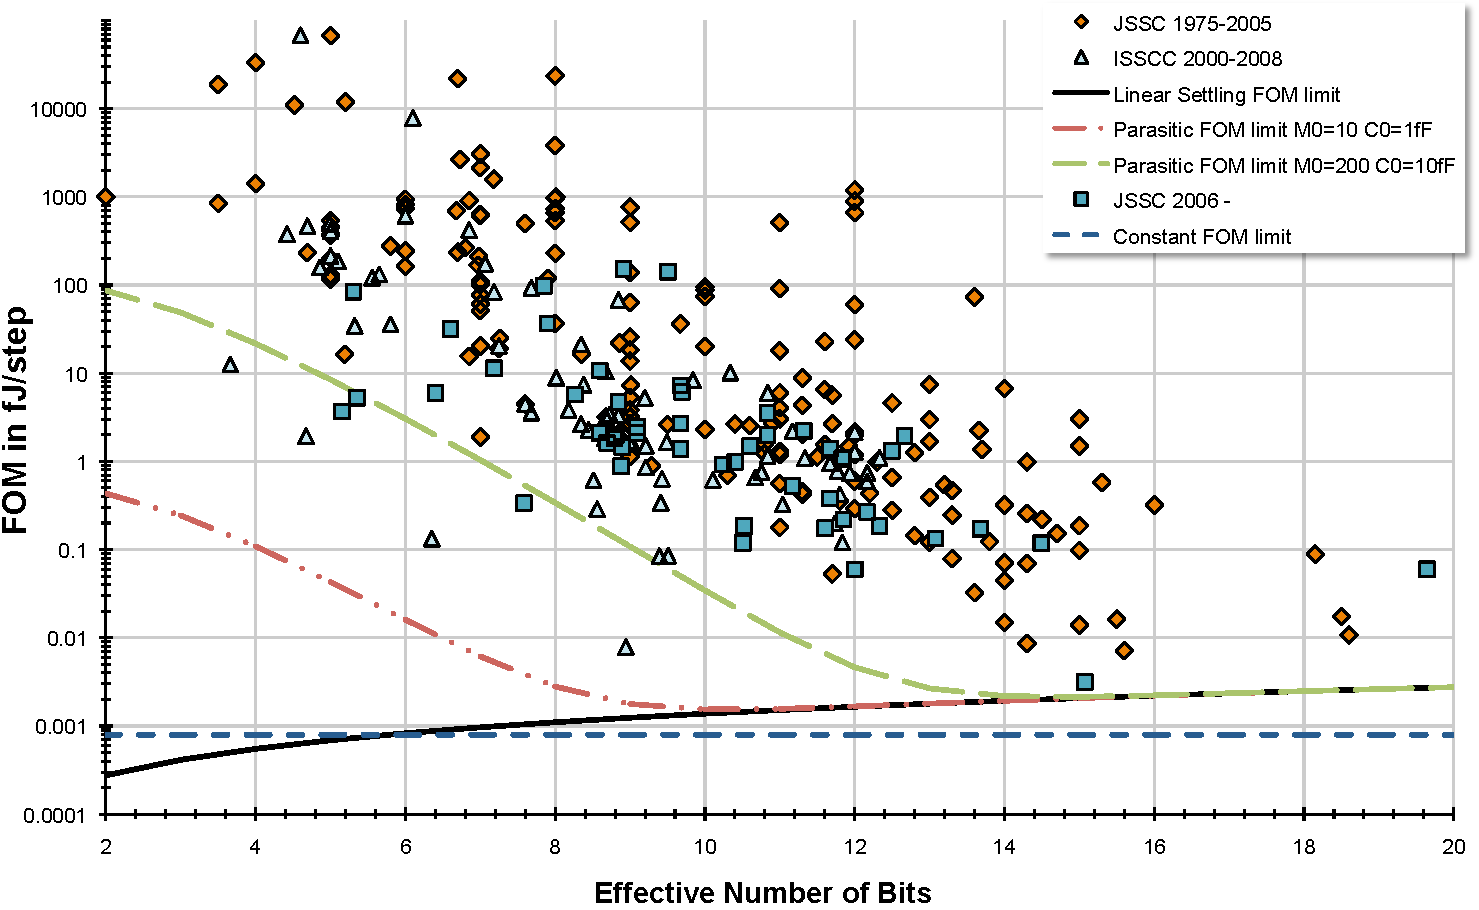
\includegraphics[width=\myfigwidthl]{graphics/adcfom}
  \caption{FOM versus bits for selected ADCs published in JSSC in the
  years 1975-2008 and ADCs published at ISSCC 2000-2008 compared to:
  the FOM limit for constant ramp, FOM limit for linear settling, and the parasitic FOM model}
  \label{fig:fomadcs}
\end{figure}


%%% Local Variables: 
%%% mode: latex
%%% TeX-master: "../../wulff/work/ntnu/phd/thesis/tb_limits"
%%% End: 


\chapter{Research Overview}\label{sc:research}

The research in this thesis is presented in seven papers. 
Fig. \ref{fig:papers} shows how the papers are related. Papers 1, 2,
4, 5 and 6 are published works, while
3 and 7 are submitted for publication. The format of all papers have been
modified to suit this thesis. The references for each paper has been
included into the complete reference list at the end of the
thesis. The content of papers 1, 2, 4, 5 and 6 have
not been modified in any way from the published version.

The topic of the research is efficient ADCs in
nano-scale CMOS technology. We focus on two separate paths:
\begin{enumerate}
\item Assume switched-capacitor implementation challenges will be
  solved and investigate ADCs with sigma-delta modulator front-end and pipelined back-end.
\item Investigate efficient circuit solutions for pipelined ADCs

\end{enumerate}
The first path include papers 1, 2 and 3 while the second path
include papers 4, 5, 6 and 7. We will describe the two paths separately.

\begin{figure}[htbp]
\centerline{ 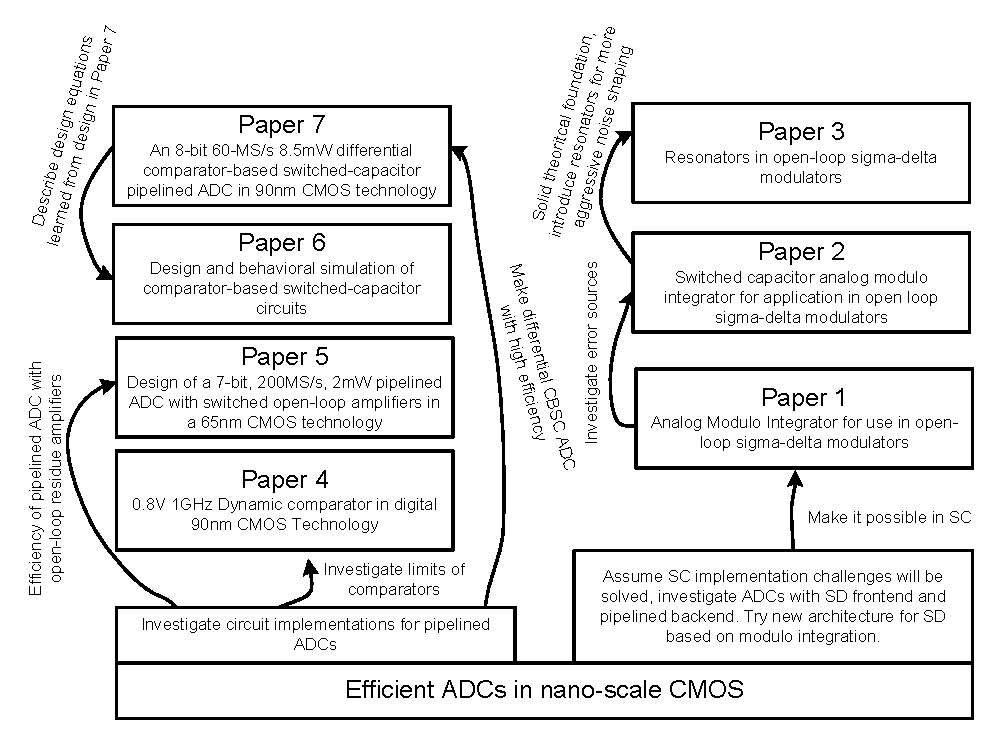
\includegraphics[width=\myfigwidthm]{graphics/paperrel}}
  \caption{How papers relate to each other and the central theme}
  \label{fig:papers}
\end{figure}

%\newpage

\section{Open-loop sigma-delta modulators (OLSDM)}
The open-loop sigma-delta
modulators in this thesis brings the OLSDM architecture to
switched-capacitor architectures. Our motivation for creating an OLSDM
is the use in hybrid converters. The idea is to use an OLSDM front-end and pipelined ADC
back-end. Such hybrid converters can achieve good performance
\cite{brooks97}. 
Previous OLSDM architectures have been digital-to-analog
modulators \cite{wisland03a}, or frequency sigma-delta modulators \cite{hovin97}. 

%Paper 1 introduce the
%switched-capacitor modulo integrator and how it could be used in an
%OLSDM. In paper 2, which is an invited paper based on paper 1, we go
%into detail on some of the error sources in OLSDM and how they can be
%corrected for. 

%Paper 3 place the theory of OLSDM on a solid ground
%by deriving conditions for when an OLSDM is equivalent to a
%sigma-delta modulator. It also introduces the modulo resonator, and
%shows an example of a 13-bit ENOB modulator with an OSR of
%4. 

Fig. \ref{fig:olsdmvspipe} shows an example of why we believe an
OLSDM-Pipelined hybrid might have an efficiency advantage. The figure
shows a comparison between a 14-bit pipelined ADC and a 14-bit hybrid
ADC.
A 14-bit pipelined ADC need
a sample and hold  and seven 1.5-bit stages\footnote{The
  number of stages can be reduced if more bits are
converted in each stage. This requires more comparators in each stage,
a 1.5-bit pipelined stage has two comparators. The accuracy of a
comparator in a B-bit stage must be $\pm V_{REF}/2^B$. Mismatch determine
the accuracy of the comparators, which usually limit the number of bits per
stage to 3-bits.} if we use a 7-bit back-end ADC. 
The hybrid converter has 5 stages before the back-end (no sample an hold), a saving of three
stages. The hybrid has two modulo resonators and a modulo integrator
that result in a fifth order noise transfer function.

To clarify why we believe that OLSDM can have an advantage, we will
describe some of the challenges in high-speed, high-accuracy
converters. These are:

\begin{description}
\item[Clock skew]  In pipelined ADCs clock skew between  the sub-ADCs and the
  sampling network (input switches and sampling capacitors) is a challenge. This skew (difference in delay) cause a signal dependent
  offset. The problem can be alleviated by placing a sample and hold
  before the first stage.

In the hybrid only the sampling capacitors are connected to the
input. Thus, clock skew is not a problem and the
hybrid does not need a separate sample and hold. 


\item[Capacitor size] In a 14-bit pipelined converter with low signal swing
 the capacitor size can be large. For 1V peak-to-peak input swing the
  input capacitance has to be 53pF (from \req{cap}). In 90nm CMOS this
  capacitance will measure 163$\mu$m by 163$\mu$m, which is a large
  area. 

The
  capacitor size can be reduced by oversampling.
  In the hybrid example in Paper 3 the oversampling ratio is four, accordingly the
  sampling capacitors can be reduced by a factor of four (13pF). 

\item[Opamp DC gain] is a significant challenge, and it is equivalent in
  the hybrid and pipelined ADC. The
error introduced by finite opamp gain cause static 
non-linearities in a pipelined ADC|this limits the accuracy of the
converter to
below the gain of the first opamp.

 In the hybrid the
finite opamp
gain
cause leakage of quantization error from each modulo integrator. The error is
shaped by the preceding signal transfer function. As a result, the
opamp gain can be scaled differently than in a pipelined ADC. 

%\item[Capacitor mismatch] is a challenge that is the same in the two
%  architectures. 

\item[ADC speed] translate into opamp branch current. The hybrid runs four
  times faster than the pipelined ADC, but has four times less
  capacitance, which cancel  with respect to current consumption. But the hybrid has a
  switched-capacitor circuit with at least three clock phases, compared to
  two clock phases for pipelined ADC. Assuming the settling requirements are
  the same for the pipelined ADC and the hybrid, the hybrid opamps must be 1.5 times faster than in the
  pipelined ADC. Preliminary simulations suggest that the hybrid will
  require opamps even faster than this, but a thorough study
  is left for future work.
\end{description}


\begin{figure}[htbp]
\centerline{ 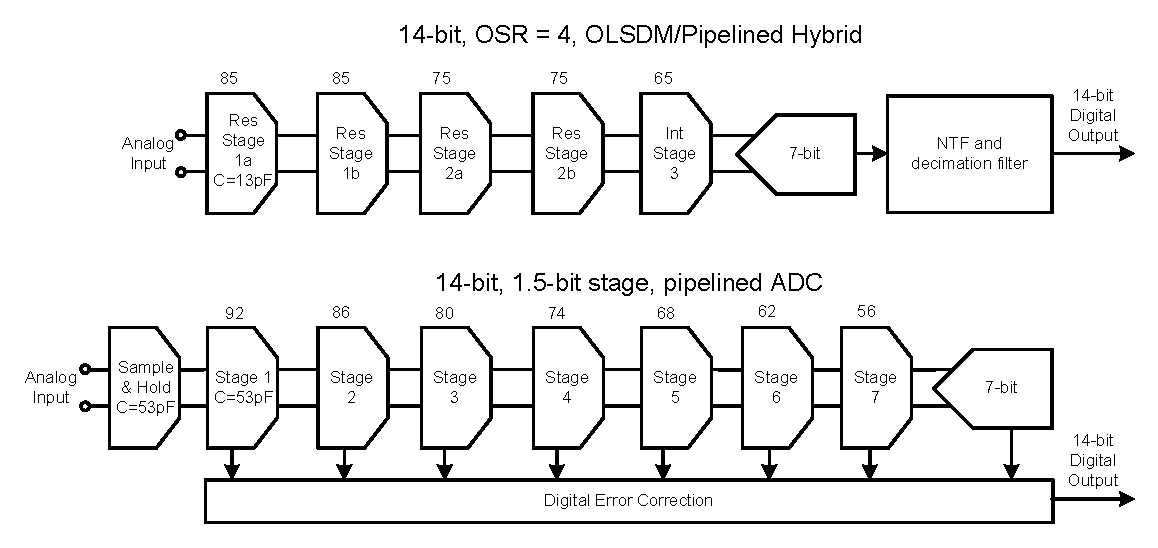
\includegraphics[width=\myfigwidthm]{graphics/olsdmvspipe}}
  \caption{Comparison between a 14-bit high-speed OLSDM and a 14-bit
    pipelined converter. The numbers above the stages denote the
    required operational amplifier
    DC gain in dB.}
  \label{fig:olsdmvspipe}
\end{figure}


\subsubsection{Paper 1: Analog Modulo Integrator For Use In Open-Loop Sigma-Delta
  Modulators}

In this paper we introduce the switched-capacitor modulo
integrator. The modulo integrator makes it possible to design an
open-loop sigma-delta modulator. The theory of OLSDM and
analog modulo integration is explained and verified through simulation.


\subsubsection{Paper 2: Switched Capacitor Analog Modulo Integrator For Application
  In Open Loop Sigma-Delta Modulators}
Paper 2 is an invited paper based on Paper 1, hence there is some
overlap in the areas covered. Paper 2 discuss one of the error effects
in OLSDM (false modulo) and investigate effects of a non-linear
quantizer.
Behavioral level simulations in SPICE of the analog modulo
integrator verify the function, and prove the concept of
amplitude modulated OLSDM.




\subsubsection{Paper 3: Resonators In Open-Loop Sigma-Delta Modulators}

In  Paper 3 we introduce the modulo resonator for 
use in open-loop sigma-delta modulators. The OLSDM 
presented in this work is intended for use in high accuracy (14- 
bit), high-speed ADCs. 
The modulo resonator is used with a modulo notch filter 
to insert a zero in the noise transfer function at a non-zero 
frequency. 
The effect of finite gain in modulo integrators and modulo 
resonators are described and verified through simulation. 
The modulo resonator and previously published modulo integrator are
used in a behavioral model of a switched-capacitor  
fifth-order OLSDM with more than 13-bit effective number of 
bits for an oversampling ratio of four.

 We prove for the N-order 
OLSDM that the number of bits in the quantizer (B) must be 
larger than N to ensure equivalence between OLSDM and sigma-delta modulation. 



%\newpage
\section{Efficient circuit solutions for pipelined ADCs}
%The pipelined ADC architecture is a popular ADC architecture  for 8-bit to 15-bit converters with speeds
%from 10MS/s to 1GS/s.
Circuit solutions that remove the opamp from switched-capacitor
circuits have received interest from the research community. The idea
is to replace the hard to make opamps with something more amenable to
nano-scale CMOS integration. In the papers we have focused on two
techniques; open-loop amplifiers, and comparator-based switched
capacitor circuits. Not only are these techniques more amenable to
nano-scale integration, but CBSC has been shown to have a fundamental
efficiency advantage over opamp based integration \cite{lee08}. 

We have also investigated the
comparators used in the sub-ADC in the pipelined ADCs.

% Paper 4 investigates a comparator for the sub-ADC in a pipelined ADC
% and its limitations in nano-scale CMOS. Paper 5 use open-loop
% residue amplifiers in a design of a 7-bit pipelined ADC. 
% Paper 6 introduce design equations for comparator based
% switched-capacitor circuits.
% Paper 7 is the first implementation of a differential
% comparator-based switched capacitor (CBSC) pipelined ADC.  CBSC has a
% fundamental efficiency advantage over opamp-based 
% pipelined ADC, as was shown in Chapter \ref{sc:limits} and
% \cite{lee08}.


\subsubsection{Paper 4:  0.8V 1GHz Dynamic Comparator In Digital 90nm CMOS
  Technology}

This paper present simulations of a dynamic comparator in 90nm CMOS
technology. It
shows how 90nm CMOS technology can achieve high speed at low supply
voltages. 

One of the challenges in dynamic comparators is controlling
the offset over process corners. As the signal swing scales down (due
to supply voltage scaling) the demands on comparators in pipelined ADC
become harder to fulfill, but as the paper shows, at 90nm CMOS it is
quite possible to have high-speed and low supply voltage. 



\subsubsection{Paper 5: Design of a 7-bit 200MS/s, 2mW Pipelined ADC With Switched
  Open-Loop Amplifiers In a 65nm CMOS Technology}

In this paper we present the design of a
7-bit 200MS/s pipelined ADC with switched open-loop amplifiers in a
65nm CMOS technology. As a
result of turning
off the open-loop amplifiers during sampling we reduce the power
dissipation by 23\%. The ADC achieves a SNDR
of 40dB close to the Nyquist frequency, with a power dissipation of
2mW, which results in a 
Walden FOM of 0.13pJ/step and a Thermal FOM of 1.6fJ/step.

%This FOM is good compared to other converters. The paper proves that low resolution converters can be
%efficiently designed as pipelined ADCs. 

%At ISSCC 2008 a analog-to-digital converter
%was presented that eclipsed the performance of any previous low
%resolution ADC
%\cite{vanderplas08} (7-bit 150MS/s 0.133 $\mu$W). But the
%architecture requires $2^{B-1}$ comparators, and they must all have $B$
%bit resolution. Hence, the architecture is unsuited for higher
%resolution.
\subsubsection{Paper 6: Design and Behavioral Simulation of Comparator-Based Switched
  Capacitor Circuits}
This paper summarize some of the design equations derived in designing
and debugging the chip in Paper 7. It presents a method for
calculating the required 
parameters for 
comparator-based switched capacitor circuits. The parameters are
capacitance ($C$), current ($I_0$), comparator delay ($T_D$), current
source output resistance ($R_o$) and comparator threshold 
($V_{ct}$). The design equations
are verified with behavioral simulations in SPICE and MATLAB.

\subsubsection{Paper 7: An 8-bit 60-MS/s 8.5mW Differential Comparator-Based Switched-Capacitor
  Pipelined ADC in 90nm CMOS Technology}
In this paper we present the first differential comparator-based switched-capacitor (CBSC) pipelined ADC. The switched-capacitor multiplying
digital-to-analog converter (MDAC)
use current sources and a comparator to do charge transfer. Continuous
time bootstrapped switches are used in the first stage to reduce signal dependent switch
resistance. A simple calibration algorithm correct for
comparator delay variation caused by the manufacturing process. Calibration reduces
ramp overshoot, which dominate the non-linearity in CBSC ADCs. The ADC is produced in a 90nm
low-power CMOS technology. The ADC core is 0.85mm x 0.35mm, with a
1.2V supply for the core and 1.8V for input switches. The ADC
has an effective number of bits (ENOB) of 7.05-bit, and a power
dissipation of 8.5mW at 60MS/s. The ADC achieves an Waldon FOM of
1.07pJ/step and Thermal FOM of 8.09fJ/step. 


\section{Clarification of contributions}
All papers have been co-authored with my supervisor Trond Ytterdal. He
has provided valuable questions, guidance and resources. 

Two papers have been co-authored with {\O}ystein Knauserud. During spring
of 2006 he did his master thesis on OLSDM and I was his supervisor. He worked out that to do
switched-capacitor OLSDM we needed a switched-capacitor modulo
integrator. As such I worked on the problem found a viable
implementation of a 
switched-capacitor modulo integrator. He provided questions and
valuable insight. 

%All papers have been written by me, and the work performed by me.




%%% Local Variables: 
%%% mode: latex
%%% TeX-master: "../../wulff/work/ntnu/phd/thesis/tb_research"
%%% End: 

%\include{../open.loop.sigma.delta/publications/modulo.integrator/olsd}
%%%%%%%%%%%%%%%%%%%%%%%%%%%%%%%%%%%%%%%%%%%%%%%%%%%%%%%%%%%%%%%%%%%%%%%
%% Fpapers.tex
%% Description:   
%% Author:        Carsten Wulff <wulff@iet.ntnu.no>
%% Created at:    Thu Apr 24 16:58:48 2008
%% Modified at:   Sat Jul 12 17:32:56 2008
%% Modified by:   Carsten Wulff <wulff@iet.ntnu.no>
%%%%%%%%%%%%%%%%%%%%%%%%%%%%%%%%%%%%%%%%%%%%%%%%%%%%%%%%%%%%%%%%%%%%%%


\chapter{Papers}\label{sc:papers}
\pagenumbering{alph}
\section{Paper 1}
\textbf{\Large 0.8V 1GHz Dynamic Comparator In Digital 90nm CMOS
  Technology}\\
%\newline
\indent   Carsten Wulff and Trond Ytterdal\\
\indent In proceedings of the 23rd NORCHIP Conference, 2005. \\
\indent 21-22 Nov. 2005 Pages 237 - 240 
\indent Digital Object Identifier: 10.1109/NORCHP.2005.1597033\\

\newpage

\section{Paper 2}
\textbf{\Large Design of a 7-bit 200MS/s, 2mW Pipelined ADC With Switched
  Open-Loop Amplifiers In a 65nm CMOS Technology}\\
\indent Carsten Wulff and Trond Ytterdal\\
\indent In proceedings of the 25th NORCHIP Conference, 2007.\\
\indent Nov. 2007\\
\indent  Digital Object Identifier 10.1109/NORCHP.2007.4481042 

\newpage

\section{Paper 3}
\textbf{\Large Analog Modulo Integrator For Use In Open-Loop Sigma-Delta
  Modulators}\\
\indent Carsten Wulff, {\O}ystein Knauserud, Trond Ytterdal\\
\indent In proceedings of the 24th NORCHIP Conference, 2006.\\
\indent Nov. 2006 Pages 125 - 128\\
\indent Digital Object Identifier 10.1109/NORCHP.2006.329259 

\newpage

\section{Paper 4}
\textbf{\Large Switched Capacitor Analog Modulo Integrator For Application
  In Open Loop Sigma-Delta Modulators}\\
\indent Carsten Wulff, {\O}ystein Knauserud, Trond Ytterdal\\
\indent Analog Integrated Circuits and Signal Processing\\
\indent Springer Netherlands\\
\indent ISSN 0925-1030\\
\indent Volume 54, Number 2, Pages 121-131 Febuary 2008\\
\indent DOI 10.1007/s10470-007-9084-2

\newpage

\section{Paper 5}
\textbf{\Large Resonators In Open-Loop Sigma-Delta Modulators}\\
\indent Carsten Wulff and Trond Ytterdal\\
\indent Submitted to Transactions on Circuits and Systems\\

\newpage

\section{Paper 6}
\textbf{\Large An 8-bit 60-MS/s 8.1mW Differential Comparator-Based Switched-Capacitor
  Pipelined ADC in 90nm CMOS Technology}\\
\indent Carsten Wulff and Trond Ytterdal\\
\indent Submitted to Journal of Solid State Circuits\\

\newpage

\section{Paper 7}
\textbf{\Large Design and Behavioral Simulation of Comparator-Based Switched
  Capacitor Circuits}\\
\indent Carsten Wulff and Trond Ytterdal\\
\indent Submitted to NORCHIP 2008s\\


%%% Local Variables: 
%%% mode: latex
%%% TeX-master: "thesis"
%%% End: 

\renewcommand{\figurename}{Figure}
\renewcommand{\myfignamehead}{Figure}
\chapter{Paper 1}\label{sc:p1}
\textbf{\Large Analog Modulo Integrator For Use In Open-Loop Sigma-Delta
  Modulators}\\
\indent Carsten Wulff, {\O}ystein Knauserud, Trond Ytterdal\\
\indent In proceedings of the 24th NORCHIP Conference, 2006.\\
\indent Nov. 2006 Pages 125 - 128\\
\indent Digital Object Identifier 10.1109/NORCHP.2006.329259 \\

\renewcommand\myfigname{p3fig:}
\renewcommand\myeqname{p3eq:}

\section*{Errata}
\begin{itemize}
\item Section 4.4. second paragraph, 3`rd to last line: altough $\rightarrow$ although
\end{itemize}

%------------------------------------------------------------------------
\begin{abstract}
%------------------------------------------------------------------------
%\section{Abstract}
A switched-capacitor analog modulo integrator is presented. This analog modulo
integrator makes it possible to design  
an Open-Loop Sigma-Delta Modulator (OLSDM). The theory of OLSDM and
analog modulo integration is explained and verified through simulation.


\end{abstract}
%\myfootnote{Financial support from the Norwegian Research Council through the
%project Smart Microsystems for Diagnostic Imaging in Medicine (project
%number 159559/130) and the project ASICs for Microsystems (project
%number 133952/420) is gratefully acknowledged. }
%-------------------------------------------------------
\section{Introduction}
%-------------------------------------------------------
Sigma-Delta modulators have become a natural choice for analog
to digital conversion in applications with low to medium bandwidth
and high resolution. They are used in applications from high
resolution instrumentation systems to ADSL communication systems. The purpose of the Sigma-Delta modulator is to shape the
quantization error such that the spectral density of the quantization
noise is non-uniform, the quantization error can for example be
high-pass or bandpass filtered. 

The Low-pass Conventional Sigma-Delta Modulator (LC-SDM) in its simplest form consists of an
integrator followed by a quantizer. The quantized signal is fed back
to the input through a digital-to-analog converter and subtracted from
the input. The transfer function of the modulator will be different for the
input signal and the quantization error of the quantizer. The input
signal will normally undergo an integration followed by a
differentiation and have a transfer function close to one. The quantization error will be
differentiated and thus high pass
filtered. 

Ideally this system could be implemented by an integrator
followed by a quantizer and a differentiator. However, an ideal integrator
has infinite DC gain, and with limited input swing in analog electronic
circuits, an ideal integrator is not possible to implement. This is
the reason why feedback is used, the feedback serves to
limit the signal swing. 

Another approach to \sd modulators is the Frequency
Sigma-Delta  Modulator (FSDM) \cite{hovin97}. Here 
an amplitude to frequency modulator was used instead of an integrator, similar to what was
suggested in \cite{claasen80}. It was shown in \cite{hovin97} that the 
preprocessing in FSDM is equivalent to modulo integration. 

In \cite{wisland02} they introduced the
non-feedback Sigma-Delta digital-to-analog converter. Here the
integrator was implemented as a digital modulo integrator.

This paper introduces an analog modulo integrator for use in 
OLSDM. The outline of this paper is as follows.
Section \ref{p3modolsd} explains that OLSDM are mathematically equivalent to LC-SDM.
In Section \ref{p3modint} the analog switched-capacitor modulo
integrator is presented, to our knowledge, it is the first of its
kind. System simulations in Section \ref{p3simulation} of the OLSDM 
verify the theory. 

%-------------------------------------------------------
\section{Open Loop Sigma-Delta Modulator} \label{p3modolsd}
%-------------------------------------------------------

%-------------------------------------------------------
\subsection{Proof of Equivalence }
%------------------------------------------------------- 
The equivalence of LC-SDM and OLSDM was shown in \cite{wisland02}. 
We endeavor to explain the equivalence in a more intuitive way. 

The OLSDM has been modeled as a quasi-linear system. Quasi-linear
since the modulo integration and modulo differentiation are stepwise linear.
The quantizer has been modeled as a linear addition of noise. Figure
\ref{p3fig:modolsd} shows the complete modulator. It should
be noted that this system is similar to the system presented in
Figure 1 in \cite{claasen80}, but they used a form of FM
modulation to implement the modulo integration. 

\begin{figure}[ht]
%  \begin{minipage}[b]{0.45\textwidth}
\centering 
 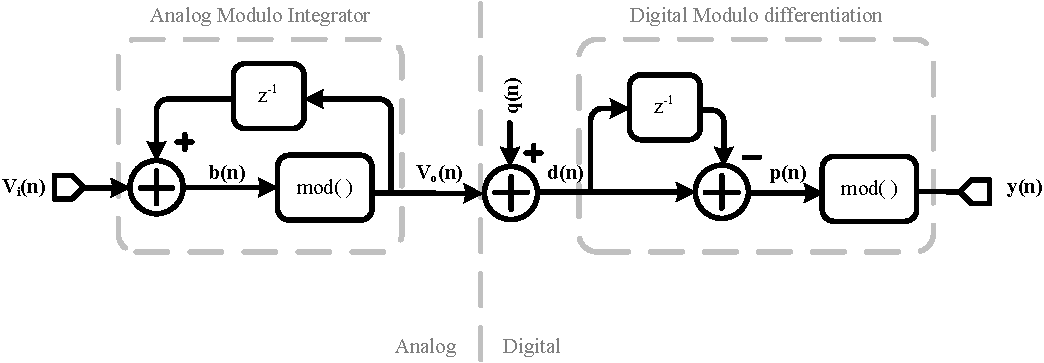
\includegraphics[width=\myfigwidth]{graphics/modolsd}
  \caption{Quasi-linear model of OLSDM}
  \label{p3fig:modolsd}
%  \end{minipage}
\end{figure}

We define the previous output from the integrator as
\eqn{
V_o(n-1) \in \langle -V_{ref}, V_{ref} \rangle
}
and the input signal as
\eqn{
\label{p3eq:rangeinput}
V_i(n) \in \langle -V_{ref}, V_{ref} \rangle
}
where $V_{ref}$ is the reference voltage.

We know that after integration, but before the modulo operation, we get
\eqn{
\label{p3eq:modintb}
b(n) = V_i(n) + V_o(n-1)
}
where $b(n)$ will be bounded by
\eqn{
b(n) \in \langle -V_{r}, V_{r} \rangle
}
where $V_r = 2V_{ref}$.
The modulo operation is used to reduce the output swing to $V_o(n) \in \langle
-V_{ref}, V_{ref} \rangle$. The modulo operation subtracts or adds
 $V_r$, depending on the value of the
summation in \req{modintb}.
The next output from the integrator can be
written as 
\begin{numcases}{V_o(n) = }
\label{p3eq:modint}
b(n) + V_r & $b(n) \in \langle -V_r, -V_{ref}]$\nonumber\\ 
b(n)  & $b(n) \in \langle -V_{ref} , V_{ref} \rangle$ \nonumber\\
b(n) - V_r & $b(n) \in [ V_{ref}, V_r \rangle$
\end{numcases}
After quantization the input to differentiation will be
\eqna{
d(n) &{}={}& V_o(n)+ q(n)\nonumber\\
d(n-1) &{}={}& V_o(n-1) + q(n-1)
}
where $q(n), q(n-1)$ are the quantization errors. 
The the output of the differentiator is
\eqn{
\label{p3eq:z(n)}
z(n) = d(n) - d(n-1)
}
If we in \req{z(n)} insert for $d(n)$, $d(n-1)$, $V_o(n)$ and set $e(n) = q(n)-q(n-1)$ the expression becomes
\begin{numcases}{z(n) = }
\label{p3eq:z2}
V_i(n) + V_r + e(n) &$V_i(n) \in \langle -V_{ref} , 0 \rangle$\nonumber\\
V_i(n) + e(n) &$V_i(n) \in \langle -V_{ref} , V_{ref} \rangle$\nonumber\\
V_i(n) - V_r + e(n) &$V_i(n) \in \langle 0 , V_{ref}  \rangle$
\end{numcases}
%The boundaries of $z(n)$, if we ignore quantization error, are given by
%\begin{numcases}{z(n) = }
%\label{p3eq:z3}
%V_i(n) + V_r  &$z(n) \in \langle V_{ref} , V_{r} \rangle$\nonumber\\
%V_i(n)  &$z(n) \in \langle -V_{ref} , V_{ref} \rangle$\nonumber\\
%V_i(n) - V_r  &$z(n) \in \langle -V_r , -V_{ref}  \rangle$
%\end{numcases}
Thus, the output of the modulator is
\begin{numcases}{y(n) = }
\label{p3eq:yn}
V_i(n) + V_r - V_r +e(n)  \nonumber\\
V_i(n) +e(n) \nonumber\\
V_i(n) -V_r +V_r + e(n) 
\end{numcases}
and for all cases in \req{yn}, $y(n) \in \langle -V_{ref} , V_{ref}
\rangle $, if we ignore the quantization error.
This gives us the well known equations
\eqn{
\frac{y(z)}{V_i(z)} = 1 \:,\:
\frac{y(z)}{q(z)} = 1- z^{-1}
}
The transfer function from the input signal to the output is one, which
is the same as for a LC-SDM (often the transfer function of a LC-SDM from input to
  output contains a time delay, $y(z)/V_i(z) = z^{-1}$ ). The quantization error is
differentiated, thus first order high pass filtered. This proof can be
extended to higher order modulators. 


%-------------------------------------------------------
%\subsection{OLSDM example }
%------------------------------------------------------- 

%An example of a conversion using the OLSDM can be seen in Figure
% \ref{p3fig:example}. Here the signals within the modulator are shown with
%their respective sample index, $n$ and $n-1$. In this example the
% quantization error is ignored for clarity, however it is shown as
%noise on the signals after quantization. The reference assigned
% an arbitrary value of $V_{ref}=3$. This value, and the other values
% in this example,  are chosen to
% correspond to the number of stacked squares in Figure \ref{p3fig:example}.  The input signal is 
%\eqn{V_i(n)  = 3 -\Delta }
%where $\Delta$ is a small value so \req{rangeinput} is satisfied. 
%After integration $b(n)$ will be given by
%\eqn{b(n) = V_i(n) + V_o(n-1) = (3 - \Delta) + 2 = 5 - \Delta}
%The output of the modulo integrator, $V_o(n)$, is
%\eqn{V_o(n) = b(n) - V_r = (5 - \Delta) -6 = -1 - \Delta}
%The signal is then quantized into $d(n)$ and $z(n)$ is
%\eqn{z(n) = d(n) - d(n-1) = (-1 - \Delta)- 2 = -3 - \Delta}
%Since $z(n) \le -V_{ref}$ the modulator adds $V_r$ and the output
%, $y(n)$, is
%\eqn{y(n) = z(n) + V_r = (-3 -\Delta) + 6 = 3 - \Delta = V_i(n)}
%Thus the output will be equal to the input plus the filtered quantization error
% as shown in \req{yn}.
%\begin{figure}[ht]
%\centering 
% 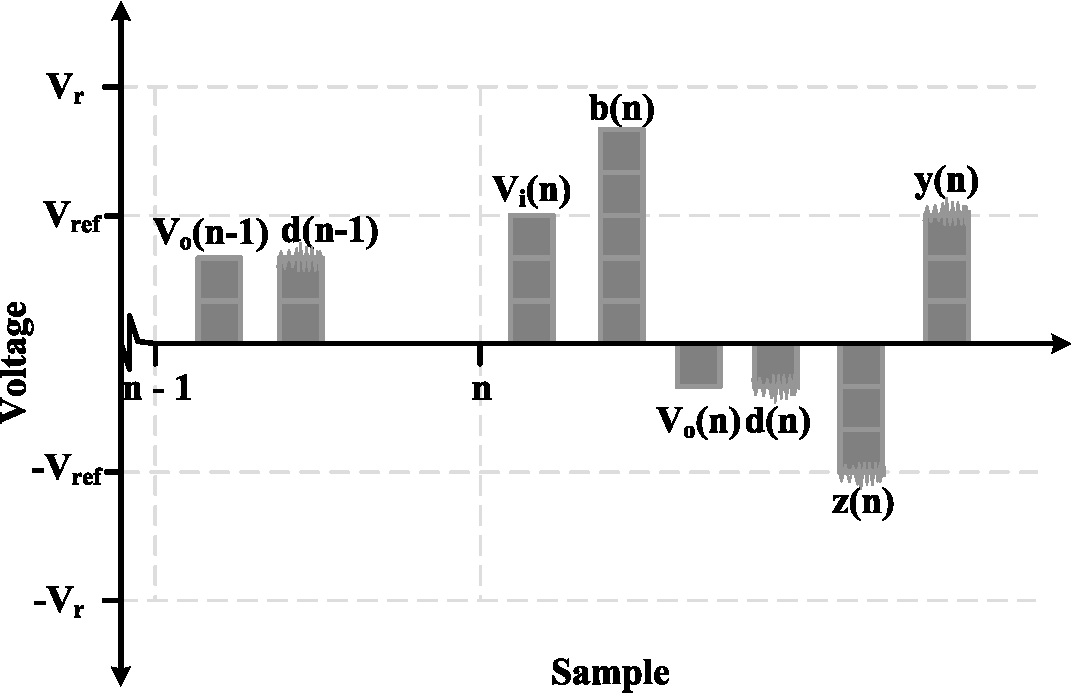
\includegraphics[width=\myfigwidth]{graphics/example}
%  \caption{Example of the modulator operation}
%  \label{p3fig:example}
% % \end{minipage}
%\end{figure}

%-------------------------------------------------------
\section{The Analog Modulo Integrator} \label{p3modint}
%-------------------------------------------------------
As shown, the modulo integrator is an integrator that resets when the output
increases or decreases beyond a reference voltage. It keeps the remainder that exceeds the reference voltage. A requirement set on the analog modulo integrator is that it should use maximum
swing available, for example 0.8V peak-to-peak with 1.2V supply. It should also be
a discrete time system. The discrete time equation for a
modulo integrator was shown in \req{modint}.

Using pseudo code the modulo integrator can be described as
\begin{enumerate}
\item Add the previous output to the current input
\item If the new output exceeds the reference voltages
\item Subtract/Add the range of the integrator, $V_r$ 
\item Set the current output to the remainder
\end{enumerate}

This is trivial to implement in the digital domain, but it may not be obvious how it
should be implemented in the
analog domain. Adding two voltages in the analog domain is conceptually
trivial. Whether a voltage exceeds a reference can be detected using a
comparator. Subtraction in the analog domain is also trivial, but
keeping the remainder presents a challenge. 

Assume that the reference voltages are
symmetric around the common mode, such that $|V_{ref}| =
|-V_{ref}|$ and $|V_{ref}|+ |-V_{ref}| = V_r$. The maximum voltage
would be less than $V_{ref} + V_{ref} = V_r$ or more than $-V_{ref} + -V_{ref} = -V_r$.  So the output after
summation, but before modulo operation, will be bounded by
\eqn{
\label{p3eq:brange}
-V_r < b(n) < V_r
}
In a circuit where the analog value is represented by voltages the swing would have to be $2V_r$ to
accuratly represent all analog values. Since our input signal has a range
of $V_r$ we would waste an extra range of $V_r$ just to represent
intermittent values in the integrator. It would be best if we could
set the voltage swing of the circuit to $V_r$, which is equal to the
maximum input swing. But in a circuit where the analog values are
represented with voltages this is difficult.

%-------------------------------------------------------
\subsection{A Solution Based on Switched Capacitors}
%-------------------------------------------------------
Switched-Capacitor (SC) circuits are prevalent in many analog
integrated circuits. In discrete time Sigma-Delta modulators it is common to
implement the integrator with a switched-capacitor circuit. It turns out that with small
modifications a switched-capacitor integrator can be converted to an analog modulo integrator. 

Realizing that in a switched capacitor integrator the analog value is
stored as charge and not as voltages is the key to understanding how a
modulo integrator can be implemented. A conventional
switched-capacitor integrator, shown in Figure \ref{p3fig:integrator}, adds the previous
output and current input. When the
integrator has settled, or failed to settle due to saturation of the opamp, it can be detected whether the output voltage
exceeds the reference voltage. If it does exceed, a charged capacitor is connected to
the charge transfer node of the integrator, node $V_g$ in Figure \ref{p3fig:integrator}. This subtracts/adds the charge
which represent $V_r$. Provided that the input signal
to the integrator never exceeds positive or negative reference, the
subtracted/added charge will bring the integrator back within bounds. Since the analog information is
stored in charge, the remainder is conserved. 

\begin{figure}[ht]
\centering 
 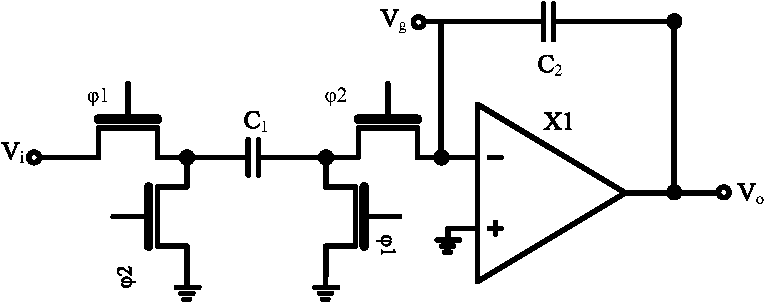
\includegraphics[width=\myfigwidth]{graphics/integrator}
  \caption{Conventional Switched-Capacitor Integrator}
  \label{p3fig:integrator}
\end{figure}

%-------------------------------------------------------
\subsection{Equations of the SC Modulo Integrator}
%-------------------------------------------------------

The circuit needed to implement a modulo integrator is shown in Figure
\ref{p3fig:moddetector}. It is connected to integrator in node $V_g$ and
$V_o$.
The complete circuit has
three clock phases; $\phi 1$, $\phi 2$ and $\phi 3$. The timing
diagram is shown in Figure \ref{p3fig:timing}, where $T$ denotes the period. 

%The analog modulo integrator can be compared to
%a first-order LC-SDM with one integrator, 1.5 bit quantizer
%and a 1.5 bit DAC. However, in the analog modulo integrator it is not the output from
%the quantizer (comparators X2 and X3 in Figure \ref{p3fig:moddetector} )
%that is used, but the analog output of the
%integrator. 

\begin{figure}[ht]
\centering 
 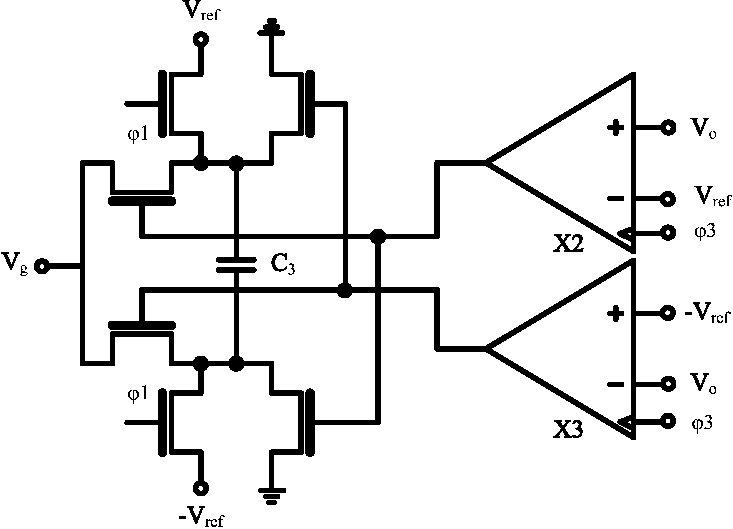
\includegraphics[width=\myfigwidth]{graphics/moddetector}
  \caption{Modulo circuit}
  \label{p3fig:moddetector}
\end{figure}

\begin{figure}[ht]
\centering 
 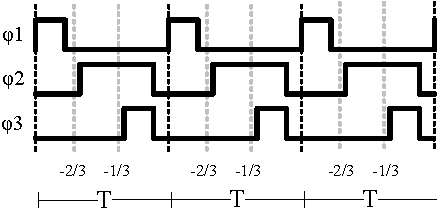
\includegraphics[width=\myfigwidth]{graphics/timing}
  \caption{Timing diagram for the modulo integrator}
  \label{p3fig:timing}
\end{figure}

Consider the integrator in Figure \ref{p3fig:integrator}, during clock phase $\phi 1$ the
input signal is sampled across capacitor C1. In clock phase $\phi
2$, before $\phi 3$, the charge from C1 is transfered to C2. The charge transfer
equation will be 
\eqn{
\label{p3eq:chargetf1}
C_2V_o(n-T/3) = C_2V_o(n-T) + C_1V_i(n-2T/3)
}
In this equation the output, $V_o(n-T/3)$, is equivalent to
$ b(n)$ from \req{modintb} and will have the same bounds, assuming $C_1 = C_2$. To make sure that the final
output, $V_o(n)$, stays within the reference voltages, $V_r$ has to be
added or subtracted as in \req{modint}.

To perform the addition/subtraction the circuit in Figure
\ref{p3fig:moddetector} is used. The different states of this circuit are
shown in Figure \ref{p3fig:moddetexpl}. During $\phi 1$, Figure
\ref{p3fig:moddetexpl} a), the capacitor $C_3$ is charged to $V_r =
V_{ref} - -V_{ref}$. During $\phi 3$ the latched comparators ( $X2$
and $X3$ in Figure \ref{p3fig:moddetector})
determine whether the output voltage exceeds the reference. Figure
\ref{p3fig:moddetexpl} b) shows the connections if the
output voltage, $V_o(n-T/3)$, is higher than $V_{ref}$. Here a charge
of $Q_3 = C_3V_r$ is transfered to the node $V_g$ in the
integrator. This will change the charge transfer equation into
\eqn{
\label{p3eq:chargetf2}
C_2V_o(n) = C_2V_o(n-T) + C_1V_i(n-2T/3) - C_3V_r
}
For $V_o(n-T/3)$ lower than $-V_{ref}$, Figure \ref{p3fig:moddetexpl}
c), the polarity of the charge is reversed and the charge transfer
function is
\eqn{
\label{p3eq:chargetf3}
C_2V_o(n) = C_2V_o(n-T) + C_1V_i(n-2T/3) + C_3V_r
}
And if $-V_{ref} < V_o(n-T/3) < V_{ref}$ the capacitor $C_3$ is not
connected to $V_g$ and the charge transfer function \req{chargetf1}
remains unchanged. Notice that the outputs from the comparators can
never be high at the same time, because $V_o(n-T/3)$ cannot be higher
than $V_{ref}$ and lower than $-V_{ref}$ at the same time.

Combining the three equations,
\req{chargetf1}, \req{chargetf2} and \req{chargetf3} with $C_1 = C_2 = C_3$ and ignoring the
frational timesteps ( $n-T/3$ and
$n-2T/3$) the result is \req{modint}.

\begin{figure}[ht]
\centering 
 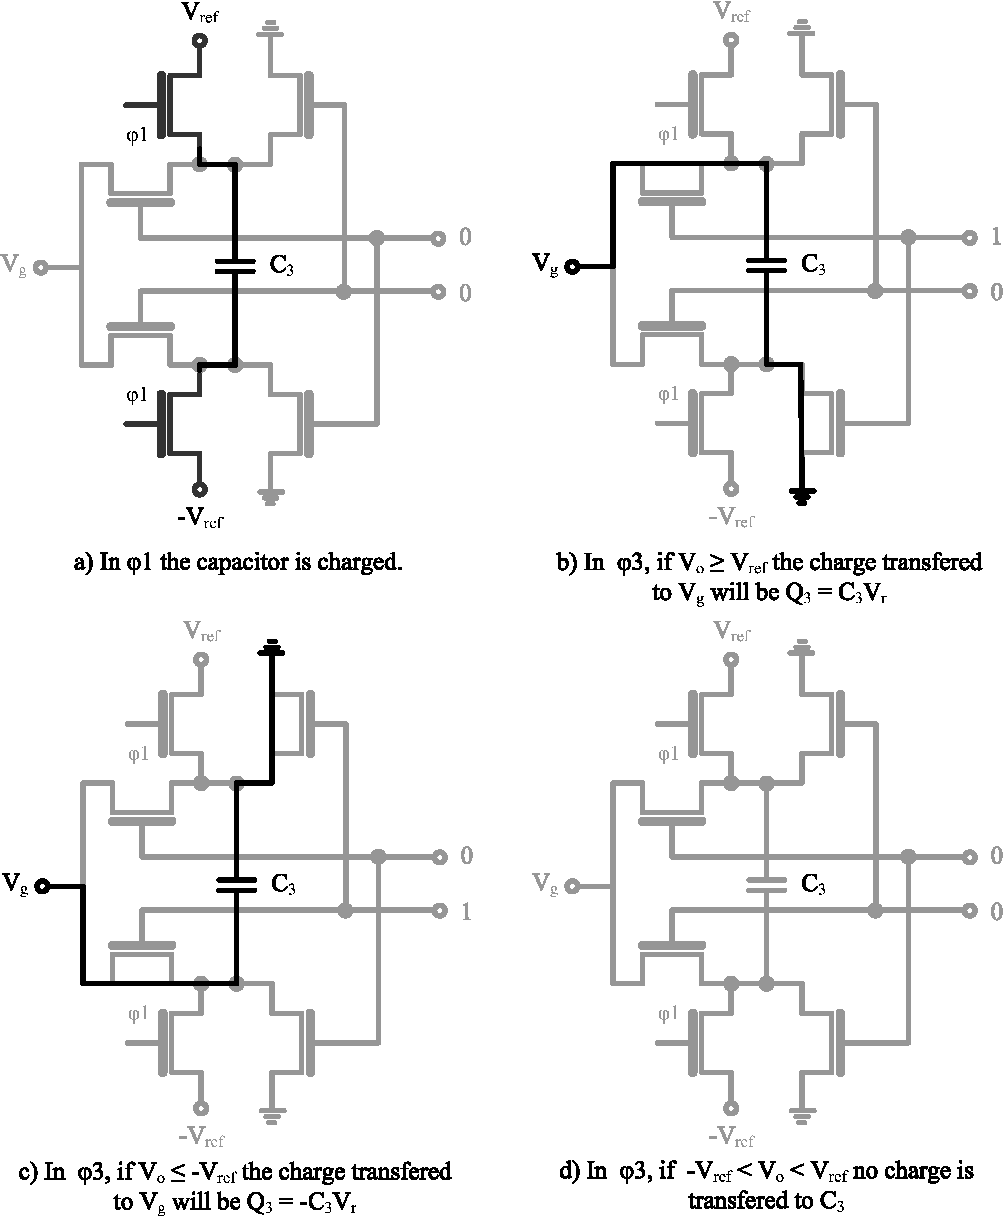
\includegraphics[width=3in]{graphics/moddetexpl}
  \caption{The different permutations of the modulo circuit}
  \label{p3fig:moddetexpl}
\end{figure}


%-------------------------------------------------------
\subsection{Simulation of the SC modulo integrator}
%-------------------------------------------------------
Simulation of the SC modulo integrator have been performed in
AimSPICE \cite{aimspice} using ideal models for comparators, switches
and operational amplifier. 

In Figure \ref{p3fig:modintdc} a DC input
signal $V_i = 0.3V$ was used, the reference voltages were set to 1V. At around $5 \mu$ the integrator
resets, here the output value would be $1.2V$ if it was not reset, and
we can clearly see that the remainder is conserved 
\eqn{-1 V + 0.2 V = -0.8V}

\begin{figure}[ht]
\centering 
 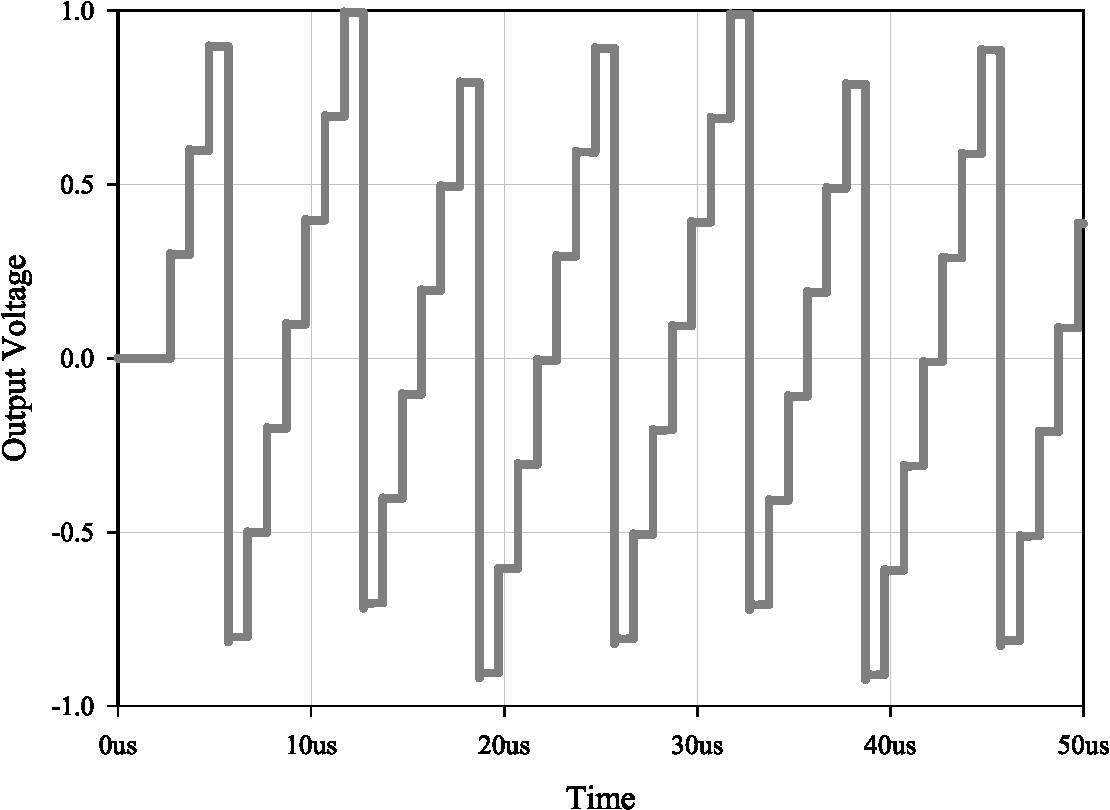
\includegraphics[width=\myfigwidth]{graphics/modintdc}
  \caption{Input vs output for the modulo integrator with constant input $V_i = 0.3V $}
  \label{p3fig:modintdc}
\end{figure}

In Figure \ref{p3fig:modintsine} the input and output for a sinusoidal
input to  the analog   modulo integrator is shown. The reference
voltage, $V_{ref}$, was set to 1V.
The sinusoidal input had an amplitude of $0.99 V$. The output has
been sampled at the end of $\phi 3$ and it can be seen how it never
exceeds the references at $V_{ref}$ and $-V_{ref}$.



%Figure \ref{p3fig:modintsine} shows the output, $V_o$, of the integrator


\begin{figure}[ht]
%  \begin{minipage}[b]{\myfigwidth}
\centering 
 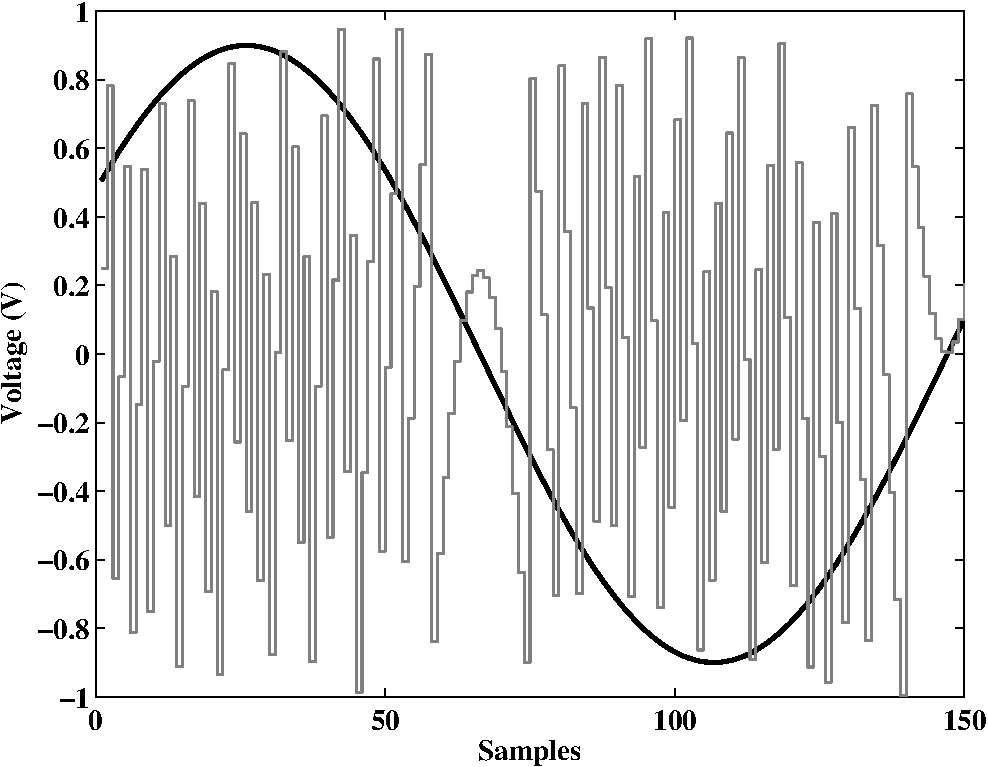
\includegraphics[width=\myfigwidth]{graphics/modintsine}
  \caption{Input vs output for the modulo integrator. Input is a sine
  with an amplitude of 0.99 V}
  \label{p3fig:modintsine}
 % \end{minipage}
\end{figure}

%-------------------------------------------------------
\section{Simulation of OLSDM Modulator}\label{p3simulation}
%------------------------------------------------------- 
The OLSDM was modeled in SystemDotNet \cite{systemdotnet05}, which is a
mixed-signal discrete-time event driven simulator. A third order
OLSDM with 8 bit quantizer was modeled. The spectral density plot can
be seen in Figure \ref{p3fig:simolsd}. From the plot we can clearly see
that we have third order high-pass filtering of the quantization
noise since the slope of the noise floor is 60dB per
decade. The dark-gray plot is an oversampled quantizer without noise
shaping, shown for comparison. With an
oversampling ratio of eight we get an ENOB (Effective Number
  Of Bits) of 15 bits. With just oversampling, no noise shaping, we
get an ENOB of 9.5 bits. 

\begin{figure}[ht]
%  \begin{minipage}[b]{\myfigwidth}
\centering 
 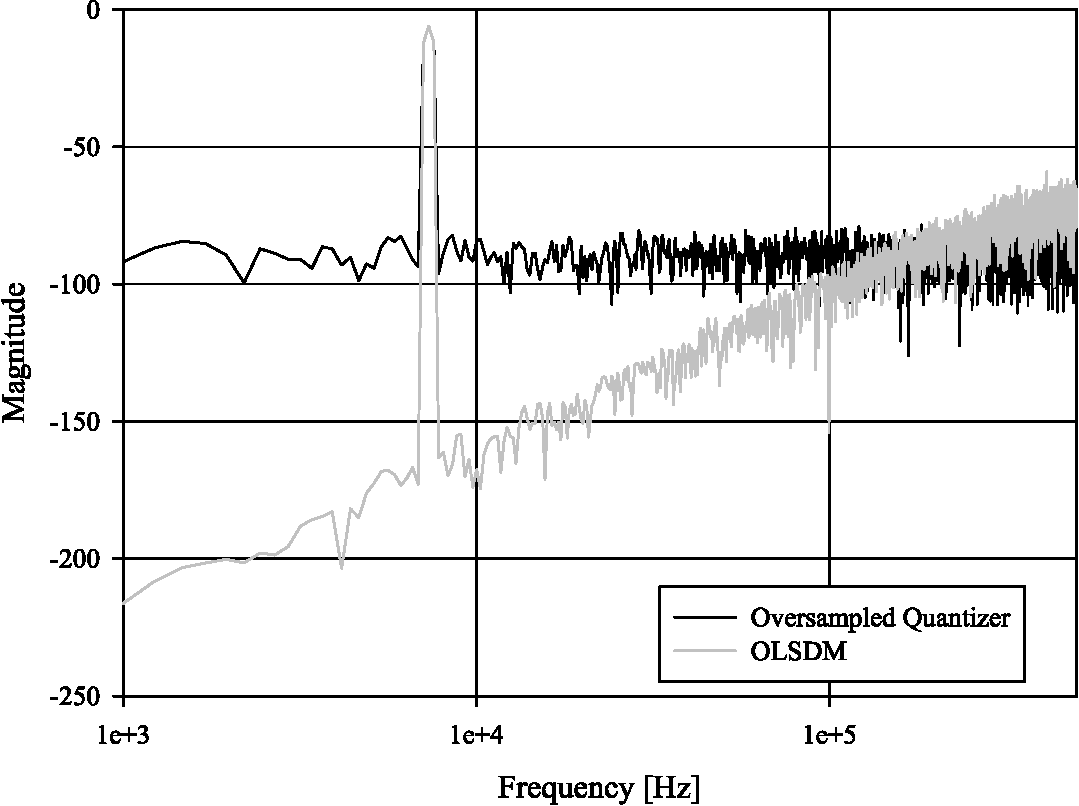
\includegraphics[width=\myfigwidth]{graphics/simolsd}
  \caption{Simulation of third order, 8 bit OLSDM. Input signal
  amplitude is $0.5$ and sampling frequency is 1MHz. Also shown is the
  output from a oversampled quantizer without noise shaping }
  \label{p3fig:simolsd}
 % \end{minipage}
\end{figure}

The analog modulo integrator can be compared to a first
order, 1.5 bit LC-SDM. In Figure \ref{p3fig:simmodint} we have
plotted the output from the OLSDM  and the combined outputs from the
comparators in the analog modulo integrator (outputs of X2 and X3 in
Figure \ref{p3fig:moddetector}). We
can clearly see that the combined output of the comparators is a first order
noise shaped version of the input signal. One could summize
that the analog modulo integrator is just a 1.5 bit LC-SDM, but that
would be inaccurate. If we assume the input signal is bounded by
\req{rangeinput}, the analog modulo integrator output will never
exceed $-V_{ref}$ or  $V_{ref}$, altough the output during $\phi2$
might saturate. For the LC-SDM the input signal swing is
normally reduced such that the output of the integrator does not
saturate.

\begin{figure}[ht]
\centering 
 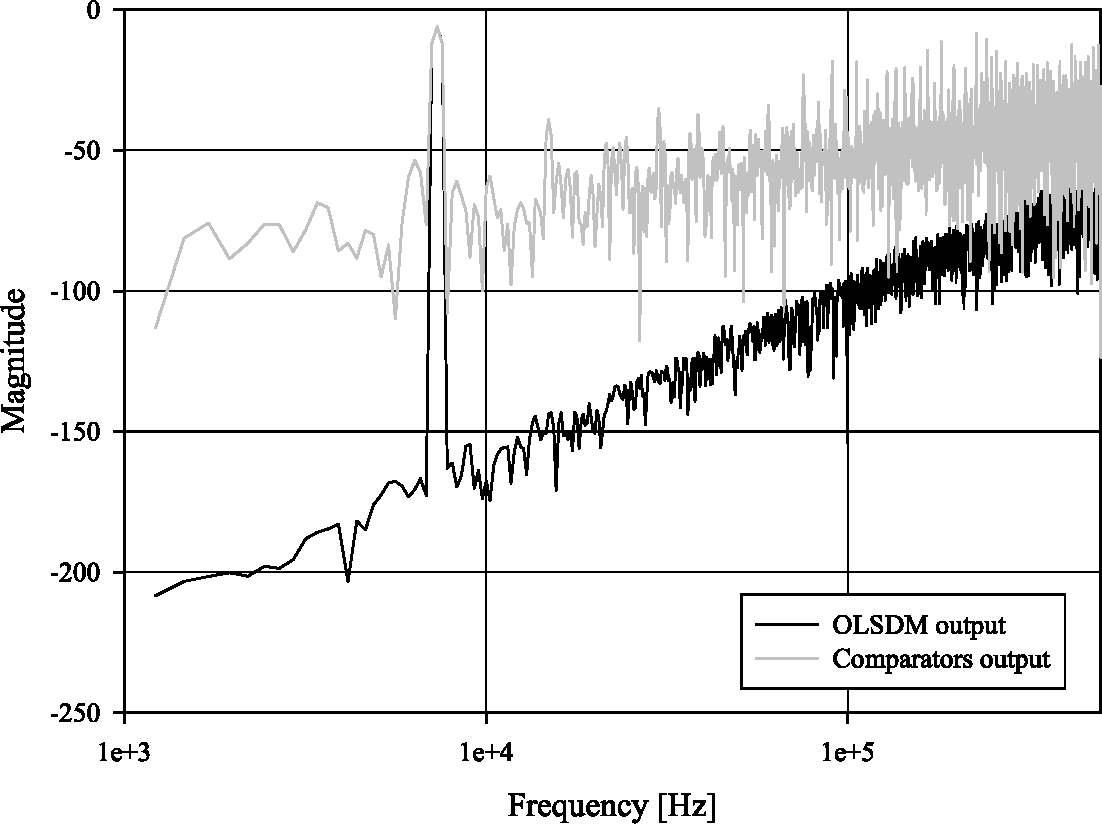
\includegraphics[width=\myfigwidth]{graphics/simmodint}
  \caption{The combined output of the comparators and the output of the OLSDM}
  \label{p3fig:simmodint}
\end{figure}

%-------------------------------------------------------
\section{Future Work}
%-------------------------------------------------------
The OLSDM architecture with analog modulo
integrator is, to our knowledge, a new architecture. Thus there are many questions to be
answered and some questions that have not yet been asked. Research is
currently being performed on the effects of mismatch, finite opamp
gain, non-linearity of quantizer, finite number of bits in quantizer,
and effects of parasitics. We hope to have an answer to some of these
questions in the near future.  
 
%-------------------------------------------------------
\section{Conclusion}
%-------------------------------------------------------
A switched-capacitor analog modulo integrator was presented. This analog modulo
integrator made it possible to design  
an Open-Loop Sigma-Delta Modulator (OLSDM). The theory of OLSDM and
analog modulo integration was explained and verified through simulation.

%------------------------------------------------------------------------
\section*{Acknowledgments}
%------------------------------------------------------------------------
{\small Financial support from the Norwegian Research Council through the
project Smart Microsystems for Diagnostic Imaging in Medicine (project
number 159559/130) and the project ASICs for Microsystems (project
number 133952/420) is gratefully acknowledged. }

%-------------------------------------------------------
%Figures
%-------------------------------------------------------



\chapter{Paper 2}\label{sc:p2}
\textbf{\Large Switched Capacitor Analog Modulo Integrator For Application
  In Open Loop Sigma-Delta Modulators}\\
\indent Carsten Wulff, {\O}ystein Knauserud, Trond Ytterdal\\
\indent Analog Integrated Circuits and Signal Processing\\
\indent Springer Netherlands\\
\indent ISSN 0925-1030\\
\indent Volume 54, Number 2, Pages 121-131 Febuary 2008\\
\indent DOI 10.1007/s10470-007-9084-2\\

\renewcommand\myfigname{p4fig:}
\renewcommand\myeqname{p4eq:}

\section*{Errata}
\begin{itemize}
\item Section 5.3.3, 5`th line: an $\rightarrow$ a
\item Section 5.3.3, second to last paragraph: We say that
  quantization noise can have codes that span the range of the
  quantizer, but this is incorrect. Quantization noise is limited to
  1LSB, so the maximum difference between two output codes with the same analog
  input is
  1LSB. This assumes that thermal noise is less than 1LSB. Thus, the
  statment in the second to last paragraph is not valid for quantizers with more than
  on bit.
\end{itemize}

%\section{Abstract}
\begin{abstract}
%------------------------------------------------------------------------
We introduce the switched capacitor analog modulo integrator, which to
our knowledge is a new circuit. We introduce
the amplitude modulated open loop \SD modulator (OLSDM), which is an analog modulo integrator
followed by a quantizer and a modulo differentiator. The mathematical
equivalence between low pass \SD modulators and OLSDM is
explained. Behavioral simulations confirm the equivalence. The
necessary circuit, a switched capacitor analog modulo integrator, is explained in detail. 
Behavioral level simulations in SPICE of the analog modulo
integrator verify the function, and prove the concept of
amplitude modulated OLSDM.

\end{abstract}

%\keywords{
\paragraph{Keywords}
 \SD Modulators, Switched Capacitor Circuits, Analog Modulo Integrator

%}
%\end{opening}        

%-------------------------------------------------------
\section{Introduction}
%-------------------------------------------------------
\SD modulators have become a natural choice for
analog-to-digital conversion in applications with low to medium
bandwidth 
and high resolution.  
The \SD modulator shapes the spectral density of the quantization error of
 data converters. 
The quantization error, or as it is often called, quantization noise,
is the error introduced by converting a continuous value signal into a
discrete value signal. This error is often considered to have uniform
spectral density, or in other words, be a white noise source. The
conditions for considering quantization error as a white noise source
was covered in \cite{widrow56}.   


The conventional low-pass \SD modulator (L-SDM) in its simplest form consists of an
integrator followed by a quantizer. The quantized signal is fed back
to the input through a digital-to-analog converter (DAC) and subtracted from
the input. The transfer function of the modulator is different for the
input signal and the quantization noise.  \footnote{This assumes a linear model of the quantizer,
  since the transfer function is only defined for a linear system} The input
signal will undergo an integration followed by a
differentiation and have a transfer function of one. The quantization noise will be
differentiated and thus high pass
filtered.

In an ideal world, with no voltage swing limitations, an L-SDM system
could be implemented by an integrator 
followed by a quantizer and a differentiator, but since supply voltage
is limited in electronic circuits, and an integrator  
has infinite dc gain, it is difficult to implement. Somehow
the output swing of the integrator has to be limited. Feedback is
normally used to limit the output swing of the integrator. 
 
There are many different types of \SD modulators. In this
paper we discuss a small sub group that we denote Open Loop \SD
Modulators (OLSDM). We define an OLSDM as: Any \SD modulator that does
not have feedback of the quantized modulator output signal.

One of the first suggestion of an OLSDM can
be found in \cite{claasen80}. Although there is no system
implementation they explain a method that avoids the feedback
DAC. More recently there have been others like the Frequency
\SD Modulator (FSDM)  in \cite{hovin97} and
\cite{wismar06}.

In the FSDM a voltage to frequency converter, a voltage controlled
oscillator (VCO), was used in place of the
integrator, and it was shown in \cite{hovin97} that the pre-processing
in FSDM is equivalent to modulo integration. The FSDM could be identified
as a frequency modulated OLSDM. 


In \cite{wisland02} they introduced the
non-feedback \SD digital-to-analog modulator where the
integrator was implemented as a digital modulo integrator. 

 In the
 past the noise shaping of \SD modulators has been combined with the
 high speed of pipelined ADCs. In \cite{brooks97} a second
 order five bit \SD Modulator was cascaded with a 12 bit
 pipelined ADC. The output of the \SD Modulator was combined with the
 output of the pipelined ADC to generate the digital output word. We
 wanted to investigate 
 whether one could avoid any interaction, with the exception of the
 input and output signals, between the \SD Modulator and the pipelined
 ADC in such a
 system. The question was; could one pre-process the input signal to
 implement the
 sigma, quantize and do post-processing to perform the delta,
 without interaction between the 
 sigma and the delta. The block diagram of such a system is shown in Figure \ref{p4fig:olsdm}

\begin{figure}[htbp]
\centerline{ 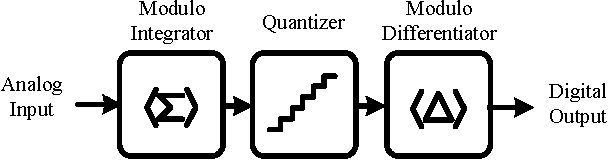
\includegraphics[width=\myfigwidth]{graphics/olsdm-sc}}
  \caption{First order OLSDM block diagram}
  \label{p4fig:olsdm}
\end{figure}


We knew from \cite{wisland02} that the open loop
 \SD modulator was  possible when all blocks were digital, by using modulo
 integration, quantization and modulo differentiation. However, in an
 analog-to-digital OLSDM the modulo integration would have to occur in
 the analog domain. 
We were unable to find any
published circuit that matched our requirements for an analog modulo integrator. Accordingly, the switched
capacitor analog modulo integrator was developed, which we present
here. To our knowledge, this switched capacitor analog modulo
 integrator is a new circuit.


In Section \ref{p4modolsd} we elaborate on the mathematical
equivalence between OLSDM and L-SDM,  which is supported by behavioral
simulations in Matlab in Section \ref{p4matlab}. Quantizer non-linearity
and common errors are also discussed in Section \ref{p4matlab}. In Section \ref{p4modint}
we introduce the analog switched capacitor modulo
integrator. Behavioral level simulations with a SPICE macro model of
the analog modulo integrator and the OLSDM are presented in Section
\ref{p4simulation}. 

%-------------------------------------------------------
\section{Open Loop \SD Modulator} \label{p4modolsd}
%-------------------------------------------------------

The most basic low pass OLSDM is an integrator, followed by a
quantizer and a differentiator as illustrated by Figure \ref{p4fig:olsdm}. The
input signal is integrated and afterwards differentiated, hence the
output is equal to the input, assuming a linear system. The quantization error added by the
quantizer is differentiated thus high pass filtered. To limit the
swing in the analog domain we use a modulo operation at the output of
the integrator. The inverse operation, which is also a modulo
operation, is performed in the digital domain after the
differentiator. A modulo operation is trivial to implement in the
digital domain. The analog modulo
operation is not trivial, and it has previously been implemented as a
voltage to frequency converter in \cite{hovin97} and \cite{wismar06}. 


The equivalence of L-SDM and OLSDM was shown in \cite{wisland02}. Here
we
endeavor to explain the equivalence more intuitively.  

The OLSDM has been modeled as a piecewise linear system.
The modulo
operation is a non-linear operation, but it can be seen as a piecewise
linear system if we ignore the discontinuities when the modulo
operation occurs. 
The quantizer has been modeled as a linear addition of noise. Figure
\ref{p4fig:modolsd} shows the complete modulator. 

\begin{figure}[htbp]
\centerline{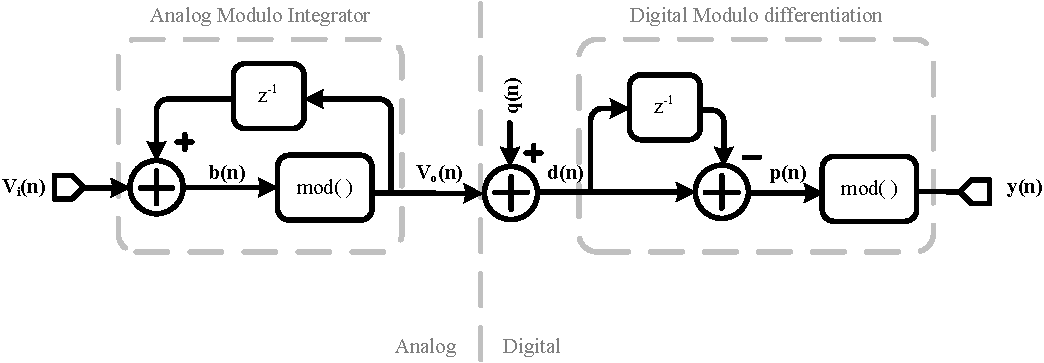
\includegraphics[width=\myfigwidth]{graphics/modolsd}}
  \caption{Piecewise linear model of the OLSDM}
  \label{p4fig:modolsd}
\end{figure}


The input signal to the modulator is $V_i(n)$, where $n$ is the sample
index. A signal with sample index $n$ is the current sample while
$n-1$ is the previous sample. The input is added to the previous
output of the integrator, $V_o(n-1)$, resulting in $b(n)$. The signal
$b(n)$ is subjected to modulo operation with $V_o(n)$ as a result.
$d(n)$ is the sum of $V_o(n)$ and the quantization noise, $q(n)$. The
differentiator output $p(n)$ is $d(n)$ minus the previous quantizer
output $d(n-1)$. To get the output, $y(n)$, $p(n)$ is subjected to a
modulo operation.  In this system the second modulo operation cancels
the first modulo operation and we have a system that is equivalent to
an L-SDM.  The equations in more detail follow.  

We define the previous output from the integrator as
\eqn{
V_o(n-1) \in \langle -V_{ref}, V_{ref} \rangle
}
and the input signal as
\eqn{
\label{p4eq:rangeinput}
V_i(n) \in \langle -V_{ref}, V_{ref} \rangle
}
where $V_{ref}$ is the reference voltage.

We know that after integration, but before the modulo operation, we get
\eqn{
\label{p4eq:modintb}
b(n) = V_i(n) + V_o(n-1)
}
where $b(n)$ will be bounded by
\eqn{
b(n) \in \langle -V_{r}, V_{r} \rangle
}
where $V_r = 2V_{ref}$.
The modulo operation is used to reduce the output swing to $V_o(n) \in \langle
-V_{ref}, V_{ref} \rangle$. The modulo operation subtracts or adds
 $V_r$, depending on the value of the
summation in \req{modintb}.
The next output from the integrator can be
written as 
\begin{numcases}{V_o(n) = }
\label{p4eq:modint}
b(n) + V_r & $b(n) \in \langle -V_r, -V_{ref}]$\nonumber\\ 
b(n)  & $b(n) \in \langle -V_{ref} , V_{ref} \rangle$ \nonumber\\
b(n) - V_r & $b(n) \in [ V_{ref}, V_r \rangle$
\end{numcases}
Accordingly \req{modint} is the equation for a modulo integrator.
After quantization the input to differentiation will be
\eqna{
d(n) &{}={}& V_o(n)+ q(n)\nonumber\\
d(n-1) &{}={}& V_o(n-1) + q(n-1)
}
where $q(n), q(n-1)$ are the quantization errors. 
The the output of the differentiator is
\eqn{
\label{p4eq:p(n)}
p(n) = d(n) - d(n-1)
}
If we in \req{p(n)} insert for $d(n)$, $d(n-1)$, $V_o(n)$ and set $e(n) = q(n)-q(n-1)$ the expression becomes
\begin{numcases}{p(n) = }
\label{p4eq:z2}
V_i(n) + V_r + e(n) &$V_i(n) \in \langle -V_{ref} , 0 \rangle$\nonumber\\
V_i(n) + e(n) &$V_i(n) \in \langle -V_{ref} , V_{ref} \rangle$\nonumber\\
V_i(n) - V_r + e(n) &$V_i(n) \in \langle 0 , V_{ref}  \rangle$
\end{numcases}

The bounds of $V_i(n)$ in \req{z2} are derived from the possible input
signal values for the modulator to reach the states in
\req{z2}. Consider the first case where 
\eqn{
p(n) = V_i(n) + V_r + e(n), V_i(n) \in \langle -V_{ref} , 0 \rangle
} Here $V_r$ has been added,
thus 
\eqn{
b(n) \in \langle -V_r, -V_{ref}]
} from \req{modint}. For b(n) to
have these bounds 
\eqn{
V_i(n) \in \langle -V_{ref}, 0 \rangle}
 and
\eqn{V_o(n-1) \in \langle -V_{ref}, 0 \rangle}
This is sufficient to
ensure the bounds of $p(n)$ in case 1 in \req{z2}  are \[p(n) \in [
V_{ref}, V_r \rangle\] Thus when we apply another modulo operation we
get 
\begin{numcases}{y(n) = }
\label{p4eq:yn}
V_i(n) + V_r - V_r +e(n)   &$V_i(n) \in \langle -V_{ref} , 0 \rangle$\nonumber\\
V_i(n) + e(n) &$V_i(n) \in \langle -V_{ref} , V_{ref} \rangle$\nonumber\\
V_i(n) -V_r +V_r + e(n) &$V_i(n) \in \langle 0 , V_{ref}  \rangle$
\end{numcases}
and for all cases in \req{yn}, $y(n) \in \langle -V_{ref} , V_{ref}
\rangle $. Equation \req{yn} can be expanded into \[y(n) = V_i(n) + q(n) - q(n-1)\]
Which result in the well known equations
\eqn{
\frac{y(z)}{V_i(z)} = 1 \:,\:
\frac{y(z)}{q(z)} = 1- z^{-1}
}
The transfer function from the input signal to the output is one, which
is the same as for an L-SDM, although often the transfer function of an L-SDM from input to
  output contains a time delay, $y(z)/V_i(z) = z^{-1}$. The quantization error is
differentiated, thus first order high pass filtered. This proof can be
extended to higher order modulators. 

%-------------------------------------------------------
\section{Behavioral Simulations In Matlab} \label{p4matlab}
%-------------------------------------------------------
The behavioral simulations presented here are an
implementation of the equations explained in the previous
section. \footnote{The Matlab code for the first and second order
  OLSDM can be downloaded from http://www.nextgenlab.net/olsdm}

%-------------------------------------------------------
\subsection{First And Second Order OLSDM}
%-------------------------------------------------------
 A first and second order
OLSDM and an oversampled quantizer without noise
shaping were modeled and simulated in Matlab. The oversampled quantizer without noise shaping was included
to compare ideal results with the simulated results. All quantizers
were implemented as 7 bit quantizers.  An oversampling ratio
(OSR) of 8 was chosen. An overview of the system can be seen in Figure
\ref{p4fig:matsys}. 

\begin{figure}[htbp]
\centerline{ 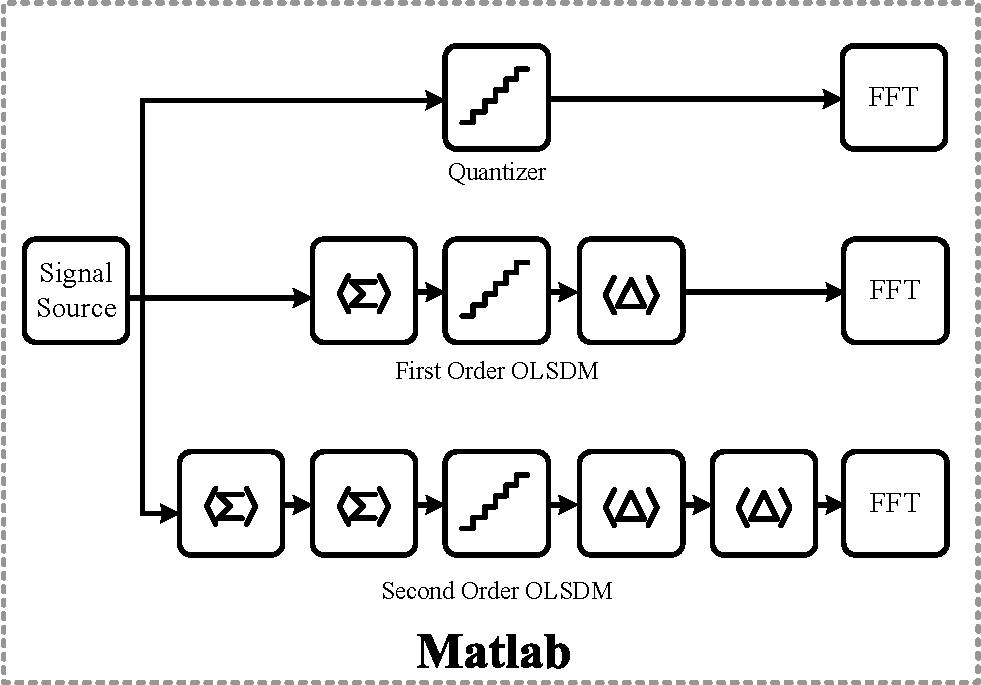
\includegraphics[width=\myfigwidth]{graphics/matsys}}
  \caption{Overview of behavioral level simulation system}
  \label{p4fig:matsys}
\end{figure}


The ideal signal to noise and distortion ratio (SNDR) for the
different cases are shown in Table \ref{p4tab:idealsndr}. The ideal SNDR
are based on equations from \cite{johns}.

\begin{table}[htbp]
\caption{ Ideal SNDR for 7 bit quantizer, OSR=8  }
\begin{tabular}{ccc}
\label{p4tab:idealsndr}
 Noise Shaping & Improvement (dB)  & Total (dB) \\ 
\hline None & $10 \times \log(OSR)$ &  52.9 \\ 
First order & $30 \times \log(OSR) - 5.17$ & 65.8 \\ 
Second order & $50 \times \log(OSR) - 12.9$ & 76.1 \\ 
\end{tabular} 
\end{table}

The equations for the OLSDM were implemented as specified in the previous section
with one exception. We chose to implement the quantizer using unsigned
integer outputs, the output ranging from 0-127. With this implementation $d(n)$ has a dc
offset. The differentiator is a high pass filter and
removes this dc offset.  For the modulo operation to work,
a dc offset was added after the differentiator to restore the correct
common mode. In the second order OLSDM a dc offset was added after
both differentiators. 

The sampling frequency was chosen arbitrarily at 1MHz and the input
signal was chosen according to the rules of coherent sampling
\cite{IEEE-1241}. In Matlab the sampling frequency is of no 
importance, we could just as well have used normalized
frequencies. However, these simulations will be compared to SPICE
simulations, and in SPICE the sampling frequency is of importance. The
input frequency was $f_{in} = 6164.6Hz$ and 
$2^{15}$ samples of the output, $y(n)$,  were calculated.

The input signal to the OLSDM must be limited, as specified in equation
\req{rangeinput}. It turns out that \req{rangeinput} is incorrect when
we deal with a finite resolution quantizer, which we will discuss in
the next section.
For the remainder of this paper the input signal amplitude has been
fixed at 0.9FSR, unless otherwise specified.
As a consequence SNDR will be 0.91dB lower than ideal cases in Table
\ref{p4tab:idealsndr}.  

The outcome of simulations are summarized in Table
\ref{p4tab:olsdmsndr}. Both the second order OLSDM and the first order
OLSDM have approximately the same SNDR as the ideal modulators. When we
remove the effects of reduced input amplitude we are left with an
error of  $+0.2dB$ for no noise shaping,  $+0.01dB$ for first order
OLSDM, and $-0.19dB$ for second order OLSDM, which is within the
errors of the SNDR extraction.  

The Fast Fourier Transform was used to
extract the SNDR, the FFTs can be seen in Figure \ref{p4fig:olsdmat} and
Figure \ref{p4fig:olsdmat2}. The light gray spectrum in the figures are the
FFTs of the ideal 7 bit quantizer, which is the same for the two figures. 

\begin{table}[htbp]
\caption{SNDR of OLSDM modulators with $2^{15}$ point FFT}
\begin{tabular}{cccc}
\label{p4tab:olsdmsndr}
 Noise Shaping & Total (dB) & Difference from Ideal (dB)\\ 
\hline
None & 52.2 & -0.7 \\ 
First order &  64.9 & -0.9 \\ 
Second order & 74.9 & -1.1 \\ 
\end{tabular} 
\end{table}

\begin{figure}[htbp]
\centerline{ 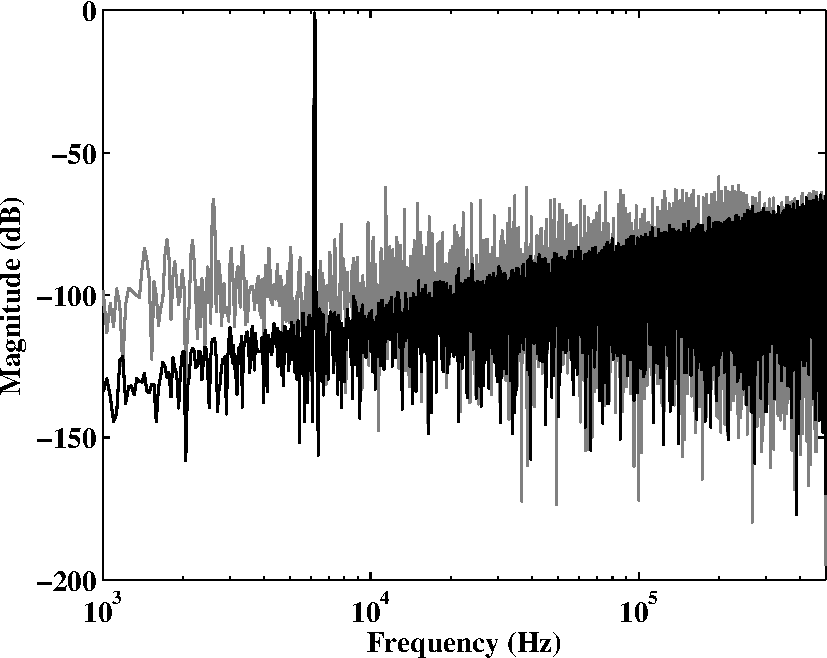
\includegraphics[width=\myfigwidth]{graphics/olsdmat} }
\caption{$2^{15}$ point FFT of the first order OLSDM output}
 \label{p4fig:olsdmat}
\end{figure}


\begin{figure}[htbp]
\centerline{ 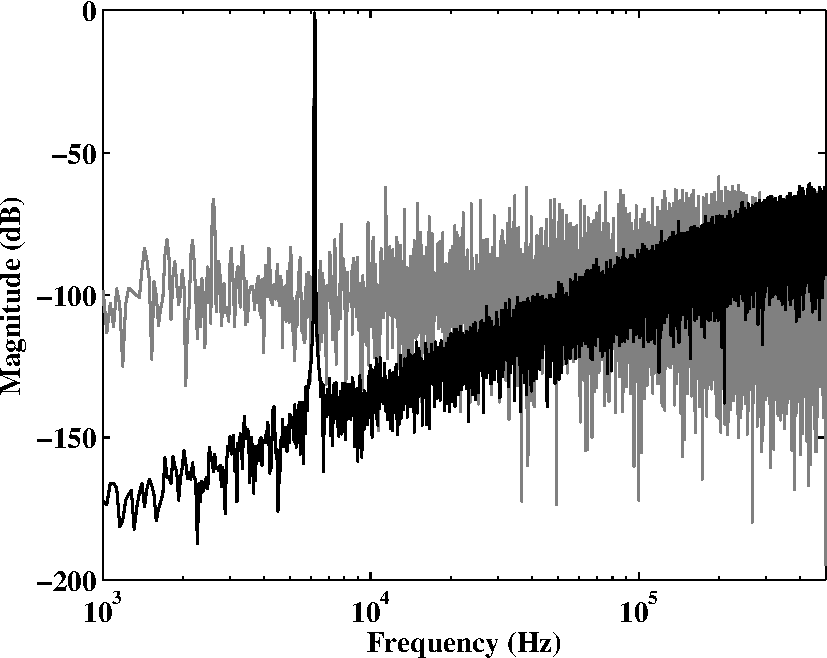
\includegraphics[width=\myfigwidth]{graphics/olsdmat2} }
\caption{$2^{15}$ point FFT of the second order OLSDM output}
 \label{p4fig:olsdmat2}
\end{figure}

%-------------------------------------------------------
\subsection{Input Signal Amplitude Limitations}
%-------------------------------------------------------
In the derivation of \req{rangeinput} we ignored quantization
noise. But when we deal with a finite resolution quantizer, quantization
noise cannot be ignored. With quantization noise \req{z2}
becomes
\begin{numcases}{p(n) = }
\label{p4eq:z2b}
V_i(n) + V_r  + e(n) &$V_i(n) + e(n) \in \langle -V_{ref} , 0 \rangle$\nonumber\\
V_i(n) + e(n) &$V_i(n) + e(n) \in \langle -V_{ref} , V_{ref} \rangle$\nonumber\\
V_i(n) - V_r  + e(n) &$V_i(n) + e(n) \in \langle 0 , V_{ref}  \rangle$
\end{numcases} 

The boundaries of \req{z2b} now include the quantization
noise. For example for case two, where \[p(n) = V_i(n) + e(n)\] no
digital modulo should be performed. To make certain no digital modulo
is performed \[V_i(n) + e(n) \in \langle -V_{ref}, V_{ref} \rangle\]
accordingly 

\eqn{
\label{p4eq:inputlimit2}
V_i(n) \in \langle -V_{ref} + |e(n)|, V_{ref} - |e(n)| \rangle
}

If the input amplitude is not limited as specified by
\req{inputlimit2}, we get a condition we denote as {\em
  false modulo} errors. For example, assume that  for case two in \req{z2b} we get 
\eqn{
p(n) = V_i(n) + e(n) <= -V_{ref}
}
as a consequence 
\eqn{
y(n) = V_i(n) + V_r + e(n)
}
here a modulo operation was carried out on $p(n)$ when it should
not have been. 

The limit in \req{inputlimit2} indicate that low resolution quantizers
may not be suited for this type of OLSDM. 

These errors are easy to spot in the output of the OLSDM, shown in Figure
\ref{p4fig:matolsdmerror}. They cause large glitches which span
the range of the output codes. To avoid these errors it is sufficient
to limit the input signal. It should be noted that the presence of
these errors completely removes the noise shaping of the OLSDM. 

In the circuit implementation of the analog modulo integrator, described by equation \req{modint},
we use comparators to detect $b(n) \in \langle -V_r,-V_{ref} ]$
and $b(n) \in [ V_{ref},V_r \rangle $. If we use the outputs from
these comparators we can prevent the {\em false modulo} errors from occuring.
In the first order OLSDM we know that a modulo
should only be performed after differentiation when a modulo
was performed in the analog modulo integrator. Consequently we can use the
outputs of the comparators in the modulo integrator to control the
modulo operation in the differentiator. 
This ensures that {\em false modulo} errors never
occur. The solution comes at the cost of delay lines that must be
added to synchronize the comparator outputs from the modulo integrators
with the modulo differentiator. For  the remainder of the paper we
do not use this solution. In Section \ref{p4falsemodulo} we describe an error correction
technique that corrects {\em false modulo} errors without using the
comparator outputs. 

Unrelated to these errors it was shown in \cite{wisland02a} that for digital-to-analog OLSDM $N+1$ quantizer bits are normally needed, where $N$ is
the OLSDM order. Thus for a second order OLSDM we would need a 3 bit
quantizer. We expect the same to be true for analog-to-digital OLSDM.

\begin{figure}[htbp]
\centerline{ 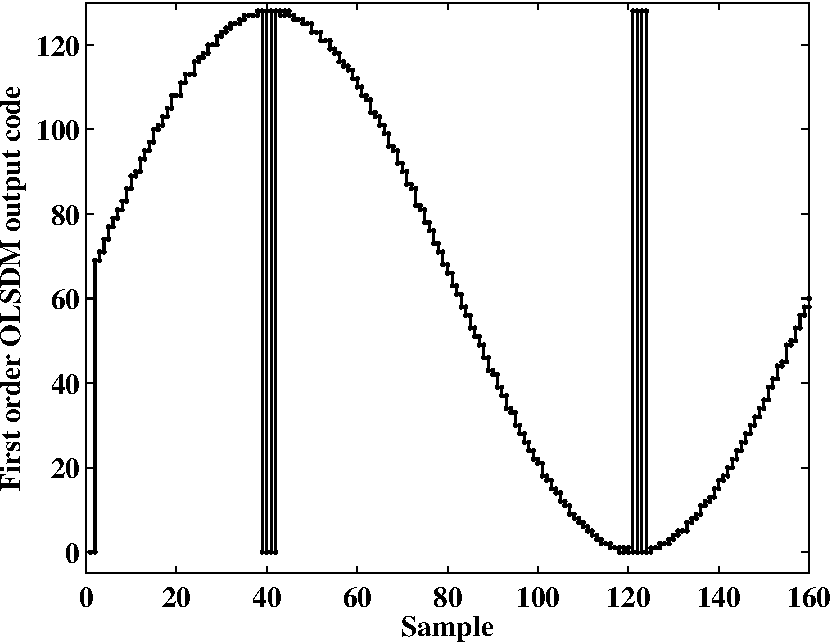
\includegraphics[width=\myfigwidth]{graphics/matolsdmerror} }
\caption{The output of the first order OLSDM in the presence of {\em false modulo} errors}
 \label{p4fig:matolsdmerror}
\end{figure}

%------------------------------------------------------
\subsection{Quantizer Linearity And Correction Of False Modulo Errors}\label{p4falsemodulo}
%------------------------------------------------------
An important issue of the amplitude modulated OLSDM is how the
linearity of the quantizer affects the system. 
The step sizes in the quantizer were made dependent on the
input signal, thus introducing a non-linearity.  By changing the
dependence on the input signal we control the linearity of the
quantizer. In this example an 7 bit quantizer with a maximum of 6.8
bit linearity was used as the quantizer in the second order OLSDM.
The results are presented for two different input amplitudes, $0.8FSR$
and $0.9FSR$. Figure \ref{p4fig:matlinolsdm2} shows
the linearity of the OLSDM as a function of quantizer
linearity. 
As expected, the linearity of the OLSDM does depend on the linearity
of the quantizer. For each bit of reduction in the linearity of the
quantizer the second order OLSDM looses half a bit of linearity. The
slope is constant until a threshold is reached, the threshold marks
the onset of {\em false modulo} errors. Below this threshold the SNDR
of the OLSDM degrades rapidly. The threshold is highly dependent on
the input amplitude and is on the order of \req{inputlimit2}.  Such a sharp
decrease in SNDR at a particular input signal amplitude is undesirable,
and it would be advantageous to correct for the cause of the sharp
degradation,  the {\em false
  modulo} errors.  As mentioned we can use the comparator output from
the analog modulo integrators to control modulo differentiation, which
will remove the {\em false modulo} errors. However, there is an alternate solution.

\begin{figure}[htbp]
\centerline{ 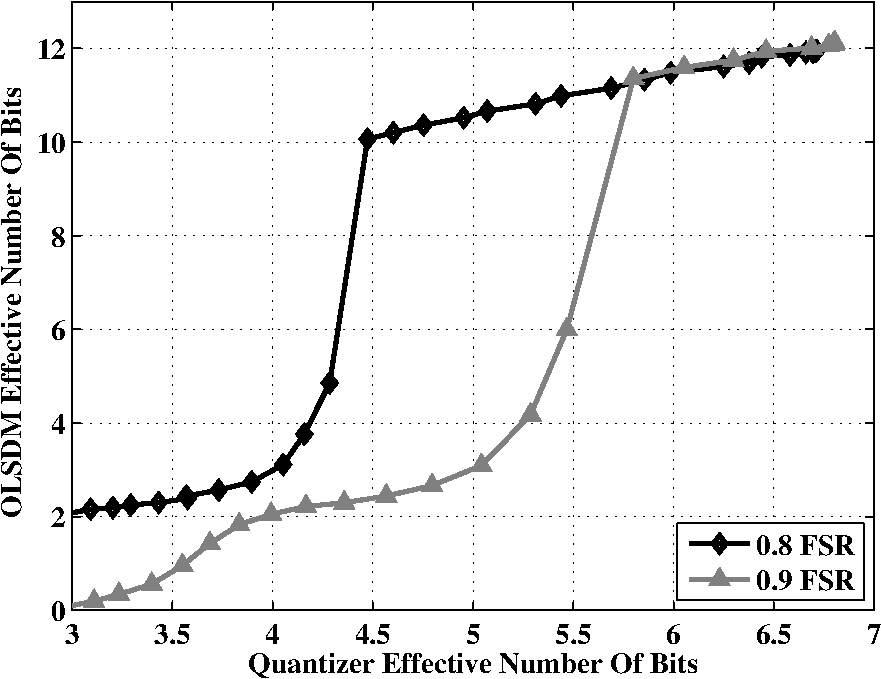
\includegraphics[width=\myfigwidth]{graphics/matlinolsdm2} }
\caption{Linearity of second order OLSDM as a function of quantizer linearity}
 \label{p4fig:matlinolsdm2}
\end{figure}

The {\em false modulo} errors have a large amplitude and high
frequency, as seen in Figure \ref{p4fig:matolsdmerror}. They span the
range of the output codes in two samples, and thus have a frequency
close to the Nyquist frequency. If we take advantage of the fact that
the input signal is, by choice, at least eight times lower than the
Nyquist frequency, since we chose an OSR of eight,  we can reduce the
errors. There is a maximum difference between two adjacent output
codes, which depend on the input signal. We assume a sinusoidal input
at one-eight of the Nyquist frequency. A sinusoid has a maximum slope
at the zero crossing which is approximately given by 
\eqn{
\label{p4eq:slopein}
 Slope  \approx A\pi/OSR
}, where A is the amplitude. In (\ref{p4eq:slopein}) we have used 
the well known assumption that $ \sin{x} \approx x $ if $x$ is
small and that $OSR = f_s/2f_{in}$. With an OSR of eight $Slope
\approx 0.39$ at zero crossing, which  is approximately one fifth of the FSR. 


We assume that any change in the output of more than $0.6FSR$ between
two consecutive samples is due to a {\em false modulo} error. 
If two consecutive samples of the OLSDM output has a difference of
more than 0.6FSR we undo the modulo operation. The result of this
simple correction can be seen in Figure
\ref{p4fig:matlinolsdm2corr}. The
error correction compensates for the dependence on input signal
amplitude and the onset of {\em false modulo} errors. It should be
noted that this error correction technique now allows the input
signal amplitude to be FSR.  

In this error correction technique we have made an assumption on the
properties of the output signal of the modulator. In this
assumption we must be cautious of the quantization noise. If we use a low
resolution quantizer the quantization noise power at higher frequencies can
be significant, and output codes which span the range of output codes
in two samples are certainly possible. Having said that, with higher
resolution quantizer and low order noise shaping the quantizer noise
power is not significant enough to influence the error correction.

\begin{figure}[htbp]
\centerline{ 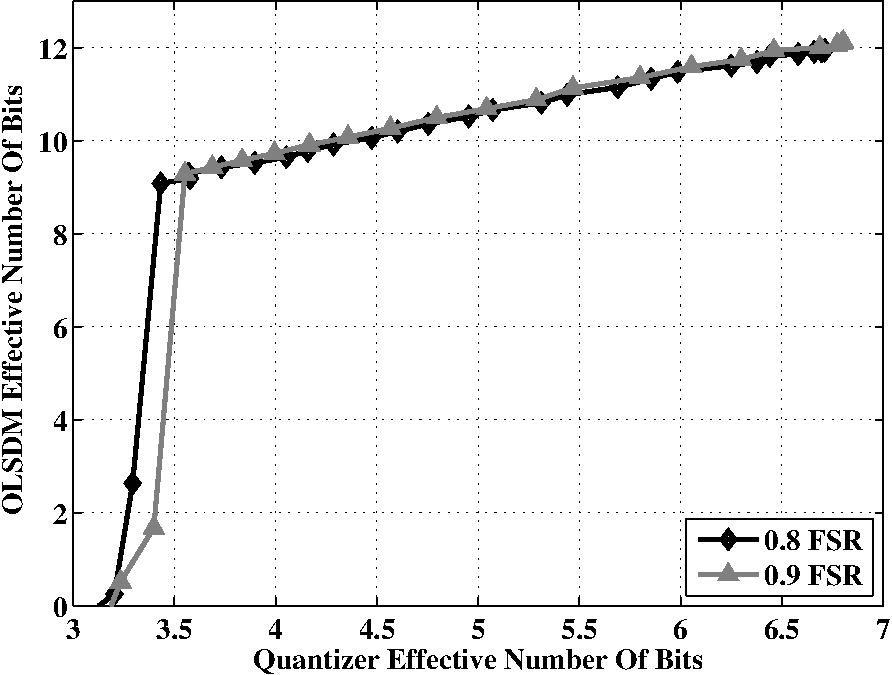
\includegraphics[width=\myfigwidth]{graphics/matlinolsdm2corr} }
\caption{Linearity of second order OLSDM as a function of quantizer
  linearity with error correction enabled} 
 \label{p4fig:matlinolsdm2corr}
\end{figure}

The circuit implementation of an amplitude modulated OLSDM requires an
analog modulo integrator. The next section explains how such a
function can be implemented by a switched-capacitor circuit.


%-------------------------------------------------------
\section{The Analog Modulo Integrator} \label{p4modint}
%-------------------------------------------------------
A requirement set on the
analog modulo integrator was that it should use maximum
swing available, for example 0.8V peak-to-peak with 1.2V supply. It should also be
a discrete time system and it should be amplitude modulated and not 
frequency modulated as was used in \cite{hovin97} and
\cite{wismar06}. The discrete time equation for a 
analog modulo integrator was shown in \req{modint}.

Using pseudo code the modulo integrator can be described as
\begin{enumerate}
\item Add the previous output to the current input
\item If the new output is equal to or exceeds the reference voltages
\item Subtract/Add the range of the integrator, $V_r$ 
\item Set the current output to the remainder
\end{enumerate}

A modulo operation is trivial to implement in the digital domain, but it may not be obvious how it
should be implemented in the
analog domain. Adding two voltages in the analog domain is conceptually
trivial. Whether a voltage exceeds a reference can be detected using a
comparator. Subtraction in the analog domain is also trivial, but
keeping the remainder presents a challenge. 

Assume that the reference voltages are
symmetric around the common mode, such that $|V_{ref}| =
|-V_{ref}|$ and $|V_{ref}|+ |-V_{ref}| = V_r$. The maximum internal
voltage in the modulo integrator  
would be less than $V_{ref} + V_{ref} = V_r$ or more than $-V_{ref} +
-V_{ref} = -V_r$.  So the output after 
summation, but before modulo operation, will be bounded by
\eqn{
\label{p4eq:brange}
-V_r < b(n) < V_r
}
In a circuit where the analog value is represented by voltages the
swing would have to be $2V_r$ to 
accurately represent all analog values. Since our input signal has a range
of $V_r$ we would waste an extra range of $V_r$ just to represent
intermittent values in the integrator. It would be better if we could
set the voltage swing of the circuit to $V_r$, which is equal to the
maximum input swing. But in a circuit where the analog values are
represented with voltages this is difficult.

%-------------------------------------------------------
\subsection{A Solution Based On Switched Capacitors}
%-------------------------------------------------------
Switched-Capacitor (SC) circuits are prevalent in many analog
integrated circuits. In discrete time \SD modulators it is common to
implement the integrator with a switched-capacitor circuit. It turns out that with small
modifications a switched-capacitor integrator can be converted to an analog modulo integrator. 

In switched-capacitor circuits the analog values are represented by
voltages across charged capacitors. A conventional
switched-capacitor integrator, shown in Figure \ref{p4fig:integrator}, adds the previous
output and current input. 

This simple integrator has two phases, sample ($\phi 1$) and charge
transfer ($\phi 2$). Assume the charge stored on $C_2$ is zero ($Q_2 = 0$). In the
sample phase we charge $C_1$ to the input voltage, thereby placing a
charge of $Q_1 = V_{i}C_1$ on the capacitor. During charge transfer
the charge of $C_1$ is transferred to $C_2$ by forcing the voltage
$V_g$ to be equal to ground using an operational amplifier. The
voltage across $C_1$ is then zero and there is no charge stored across
it, all charge is across $C_2$. This causes the output voltage to be
$V_o(n) = Q_1/C_2$. If the input value is kept constant, the next output
value, after a clock cycle, will be $V_o(n+1) = 2Q_1/C_2$. 

In the charge transfer phase $V_g$ is a high
impedance node, thus the total charge, $Q_{tot}$, given by $Q_{tot} = Q_1
+ Q_2$, does not change. $Q_{tot}$ is independent of the voltages at $V_g$ and
$V_o$. Thus we can argue that the ideal output value, $V_{o-ideal} =
Q_{tot}/C_2$ is only dependent on the total charge across the capacitors. By
ideal output voltage $V_{o-ideal}$ we mean the output voltage $V_o$ if
$V_g$ was forced to ground.

A real world operational amplifier
will normally have a maximum output signal swing. For example, if we exceed this signal swing the
gain in the operational amplifier goes down, and it is unable to force
virtual ground. In this case $V_o$ saturates, it cannot go any
higher, hence $V_o < V_{o-ideal}$. This saturation voltage we
define as $V_{sat} > V_{ref}$. 

Assume that the operational amplifier saturates in $\phi 2$, hence
$V_o = V_{sat} > V_{ref}$. If we can detect this condition, $V_o >
V_{ref}$, we can subtract a charge from $V_g$ that represents $V_r$
($V_r = 2V_{ref}$ as defined in Section \ref{p4modolsd}), thus
perform a modulo operation. We would now have \[V_{o-ideal} = (Q_{tot}-
Q_{V_r})/C_2 <
V_{ref} < V_{sat}\] as a consequence the operational amplifier will be
able to force virtual ground. 

One of the differences between the switched capacitor analog modulo
integrator and the conventional integrator is that the latter has three clock
phases. The first two have the same function as in the conventional
integrator, sample and charge transfer. The third clock phase is added
to detect if $V_o > V_{ref}$ (and the opposite, $V_o < -V_{ref}$) in phase two.
 If it does exceed, a charged capacitor
is connected to 
the charge transfer node of the integrator, node $V_g$ in Figure
\ref{p4fig:integrator}. This subtracts or adds the charge 
which represent $V_r$. This will change the charge transfer equation,
and as we shall see, implement a modulo operation. 

Provided that the input signal limited as specified by \req{inputlimit2}, the
subtracted/added charge will ensure that 
\eqn{
- V_{ref} < V_o < V_{ref}
}

\begin{figure}
\centerline{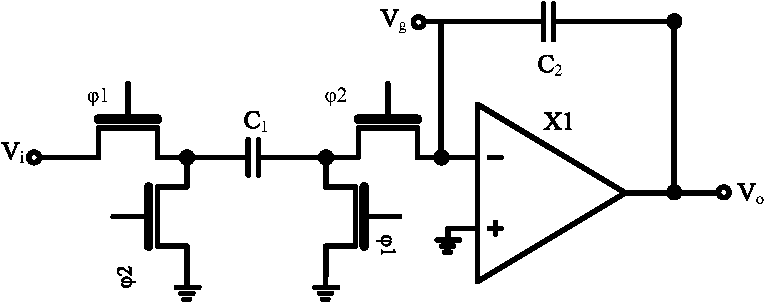
\includegraphics[width=\myfigwidth]{graphics/integrator}}
  \caption{Conventional switched capacitor integrator}
  \label{p4fig:integrator}
\end{figure}

The circuit needed to implement a modulo integrator is shown in Figure
\ref{p4fig:moddetector}. It is connected to the integrator in node $V_g$ and
$V_o$.
The complete circuit has, as mentioned,
three clock phases; $\phi 1$, $\phi 2$ and $\phi 3$. The timing
diagram is shown in Figure \ref{p4fig:timing}, where $T$ denotes the
period and $1/3, 2/3$ denotes the fractional time steps.  

\begin{figure}
\centerline{ 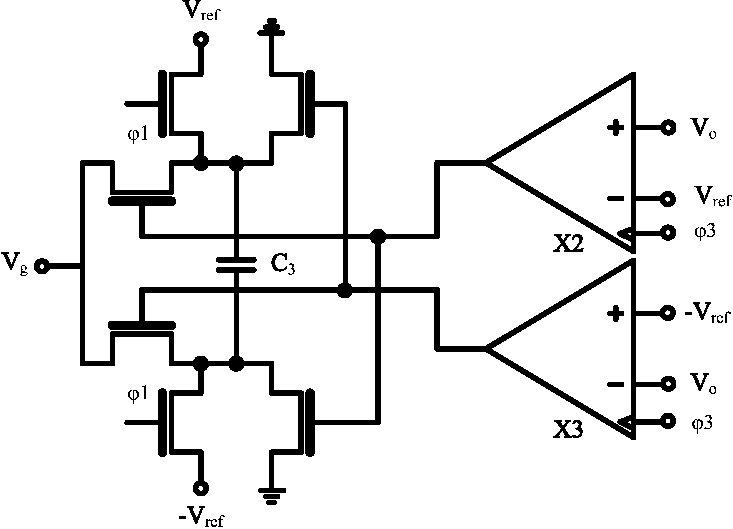
\includegraphics[width=\myfigwidth]{graphics/moddetector}}
  \caption{Modulo circuit}
  \label{p4fig:moddetector}
\end{figure}

\begin{figure}
\centerline{ 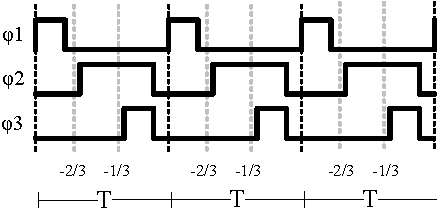
\includegraphics[width=\myfigwidth]{graphics/timing}}
  \caption{Timing diagram for the modulo integrator}
  \label{p4fig:timing}
\end{figure}


Consider the integrator in Figure \ref{p4fig:integrator}. During clock phase $\phi 1$ the
input signal is sampled across capacitor C1. In clock phase $\phi
2$, before $\phi 3$, the charge from C1 is transferred to C2. The charge transfer
equation will be 
\eqn{
\label{p4eq:chargetf1}
C_2V_o(n-T/3) = C_2V_o(n-T) + C_1V_i(n-2T/3)
}
In this equation, $V_o(n-T/3)$, is equivalent to
$ b(n)$ from equation \req{modintb} and will have the same bounds, assuming $C_1 = C_2$. For the 
output, $V_o(n)$,  to stay within the reference voltages, $V_r$ has to be
added or subtracted as in equation \req{modint}.

\begin{figure*}
\centerline{ 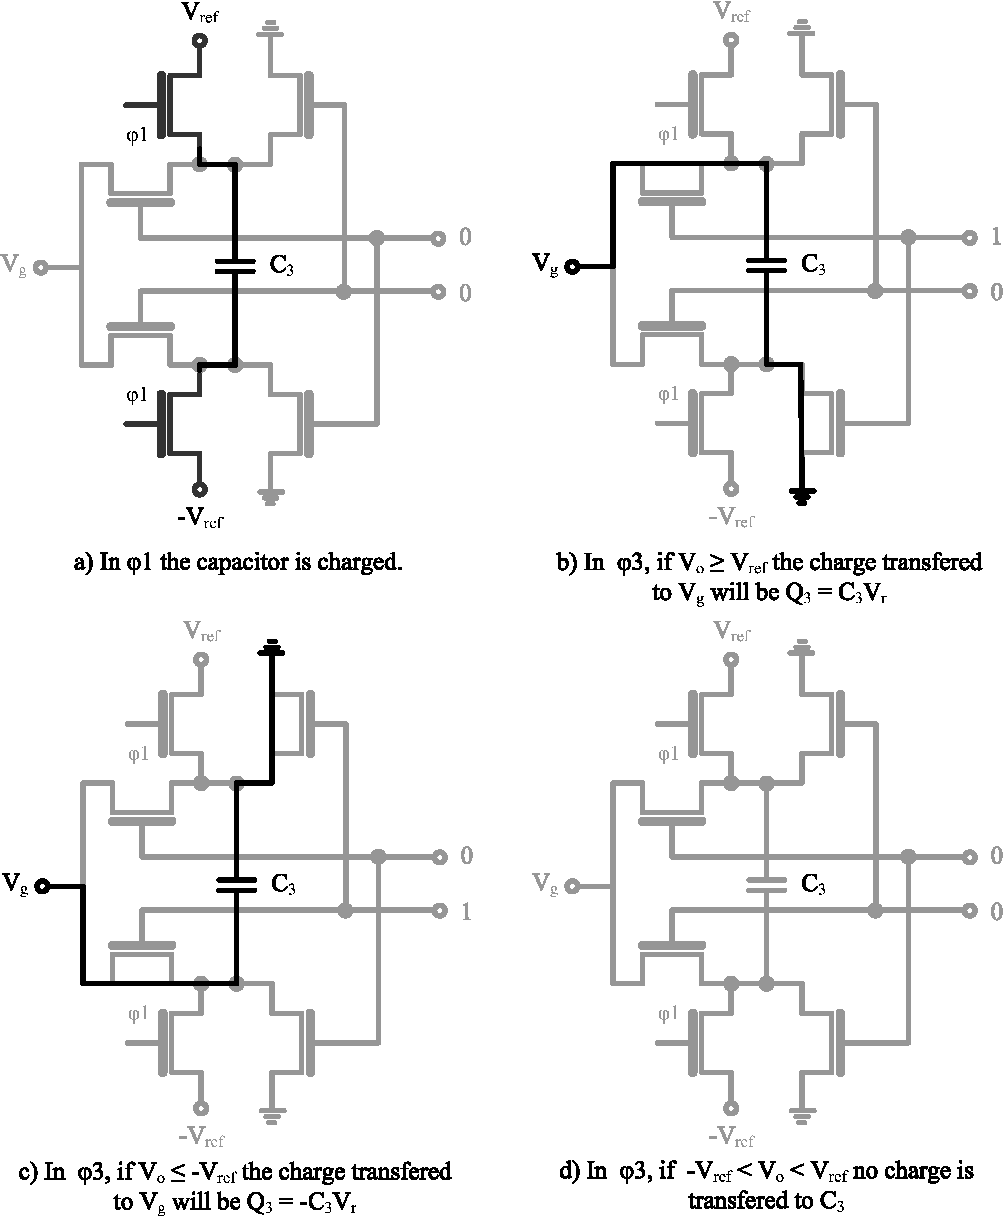
\includegraphics[width=5.5in]{graphics/moddetexpl}}
  \caption{The states of the modulo circuit in Figure \ref{p4fig:moddetector}}
  \label{p4fig:states}
\end{figure*}

Figure \ref{p4fig:states} shows the states of Figure \ref{p4fig:moddetector} in more detail. During $\phi 1$, Figure
\ref{p4fig:states} a) , the capacitor $C_3$ is charged to $V_r =
V_{ref} - -V_{ref}$. At the start of $\phi 3$ the latched comparators ( $X2$
and $X3$ in Figure \ref{p4fig:moddetector})
determine whether the output voltage exceeds the reference. Figure
\ref{p4fig:states} b) shows the connections if the
output voltage, $V_o(n-T/3)$, is higher than $V_{ref}$. Here a charge
of $Q_3 = C_3V_r$ is transferred to the node $V_g$ in the
integrator. This will change the charge transfer equation into
\eqn{
\label{p4eq:chargetf2}
C_2V_o(n) = C_2V_o(n-T) + C_1V_i(n-2T/3) - C_3V_r
}
For $V_o(n-T/3)$ lower than $-V_{ref}$, Figure \ref{p4fig:states} c) , the polarity of the charge is reversed and the charge transfer
function is
\eqn{
\label{p4eq:chargetf3}
C_2V_o(n) = C_2V_o(n-T) + C_1V_i(n-2T/3) + C_3V_r
}
And if $-V_{ref} < V_o(n-T/3) < V_{ref}$ the capacitor $C_3$ is not
connected to $V_g$ and the charge transfer function \req{chargetf1}
remains unchanged as shown in Figure \ref{p4fig:states} d). Notice that the outputs from the comparators can
never be high at the same time.

Combining the three equations,
\req{chargetf1}, \req{chargetf2} and \req{chargetf3} with $C_1 = C_2 = C_3$ and ignoring the
fractional time-steps ( $n-T/3$ and
$n-2T/3$) the result is \req{modint}.

The analog modulo integrator presented here resemble a first-order low
pass 1.5 bit 
\SD Modulator. If one plots the spectrum of the combined comparator
outputs it is a quantized first order noise shaped version of the
input. What
makes an analog modulo integrator different from a
first order low pass \SD Modulator is
\begin{itemize}
\item The quantizer levels are set at $\pm V_{ref}$, and not evenly
distributed between $\pm V_{ref}$. 
\item The three phase clock implements a
form of zero time quantizer 
feedback, if $V_o$ is higher than $V_{ref}$ $V_r$ is immediately
subtracted before the next output of the integrator.
\item The comparator outputs are not necessary to reverse the effect
  of the modulo operation in the digital domain.
\end{itemize}




%-------------------------------------------------------
\section{Behavioral Level Verification Of The SC OLSDM} \label{p4simulation}
%-------------------------------------------------------
We implemented a macro model description of the SC analog modulo
integrator described in the previous section.\footnote{The SPICE
  macro model of the switched capacitor analog modulo integrator can
  be downloaded from http://www.nextgenlab.net/olsdm} A single pole 
operational amplifier macro model
with a dc gain of 74dB and a voltage limiter was used to model
the operational amplifier. The comparators were modeled as latched
comparators. Ideal 
switches with an on resistance of 200 Ohms were used and the
capacitors C1-C3 were 5pF. The reference voltages
were $V_{ref} = 1V$ and $-V_{ref} = -1V$. The switch resistance, capacitance
and references were chosen arbitrarily. The output of the
operational amplifier was limited to $\pm 1.4V$. This ensures that for
some values of the input the integrator will saturate during $\phi
2$. The input frequency,
sampling frequency and the number of samples was the same as for the
Matlab simulation. An overview of the system can be seen in
Figure \ref{p4fig:matspice}. 

\begin{figure}[htbp]
\centerline{ 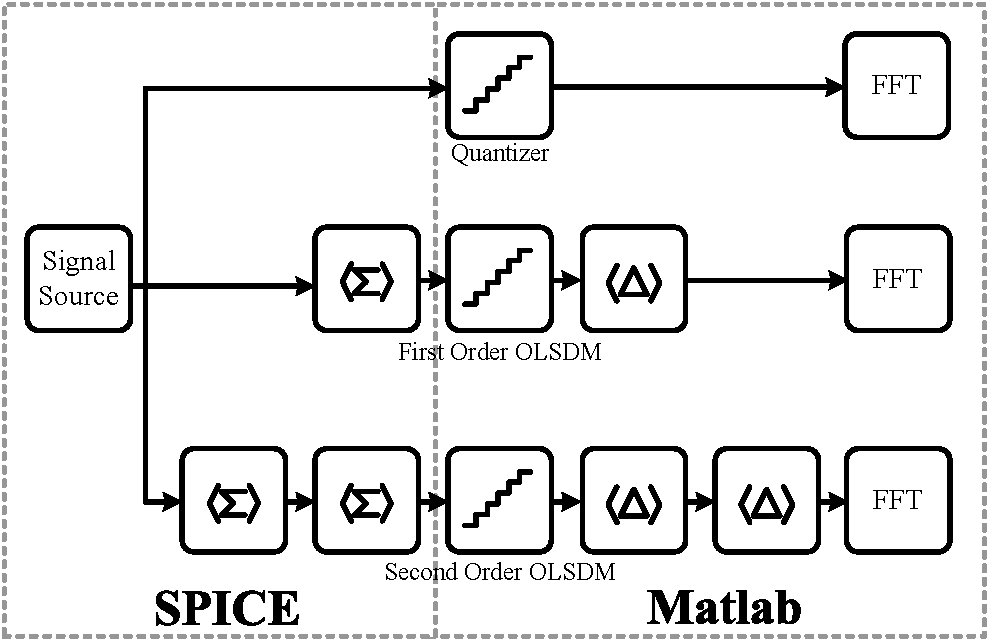
\includegraphics[width=\myfigwidth]{graphics/matspice}}
  \caption{Overview of circuit simulation with macro models}
  \label{p4fig:matspice}
\end{figure}

Only the analog modulo integrator was implemented in SPICE. Its output
was extracted and post-processed in Matlab. The code for the
differentiator and the quantizer were the same as in the behavioral
simulations. 

In Figure \ref{p4fig:modintsine} the input signal (dark gray) and the
output signal (light gray) of the first order SC modulo integrator is shown for
the first 150 samples. The sinusoidal input had an amplitude of $0.9
V$. The output, $V_o$, has 
been sampled at the end of $\phi 3$ and it can be seen how it never
exceeds the references at $V_{ref}$ and $-V_{ref}$.

\begin{figure}[htbp]
\centerline{ 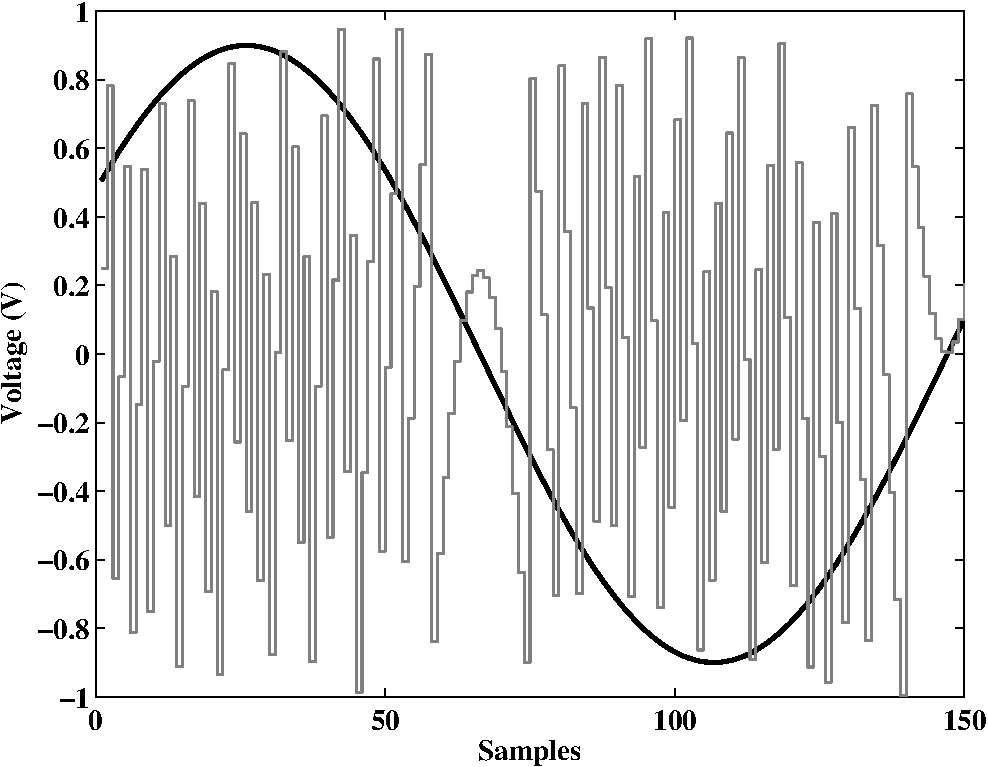
\includegraphics[width=\myfigwidth]{graphics/modintsine}}
  \caption{Input vs output for the modulo integrator. Input is a sine
  with an amplitude of 0.9 V}
  \label{p4fig:modintsine}
\end{figure}

A transient simulation was performed. The results are summarized
in Table \ref{p4tab:olsdmsndrspice}. If we remove the effect of reduced
input signal amplitude the errors are $-0.2dB$ for first order OLSDM
and $-2.1dB$ for second order OLSDM. The error for first order OLSDM
is within the error of the SNDR extraction. The error for the second
order OLSDM it is to large to be caused by deviations due to SNDR
extraction. This extra loss of $-2.1dB$ was mainly due to non-linearity
of the voltage limiter used in the simulation. When the voltage
limiter is removed the error for second order OLSDM is reduced to
$-0.79dB$. The remaining difference is mostly due to finite gain in the
operational amplifier. The FFTs of the first and second order OLSDM are
shown in Figure \ref{p4fig:olsdmspice} and Figure \ref{p4fig:olsdmspice2},
the ideal quantizer in light gray and the OLSDM output in dark gray. 

\begin{table}[htbp]
\caption{ SNDR of OLSDM modulators in SPICE}
\begin{tabular}{cccc}
\label{p4tab:olsdmsndrspice}
 Noise Shaping & Total (dB) & Difference from Ideal (dB)\\ 
\hline 
First order &  64.7 & -1.1 \\ 
Second order & 73.1 & -3 \\ 
\end{tabular} 
\end{table}

 \begin{figure}[htbp]
\centerline{ 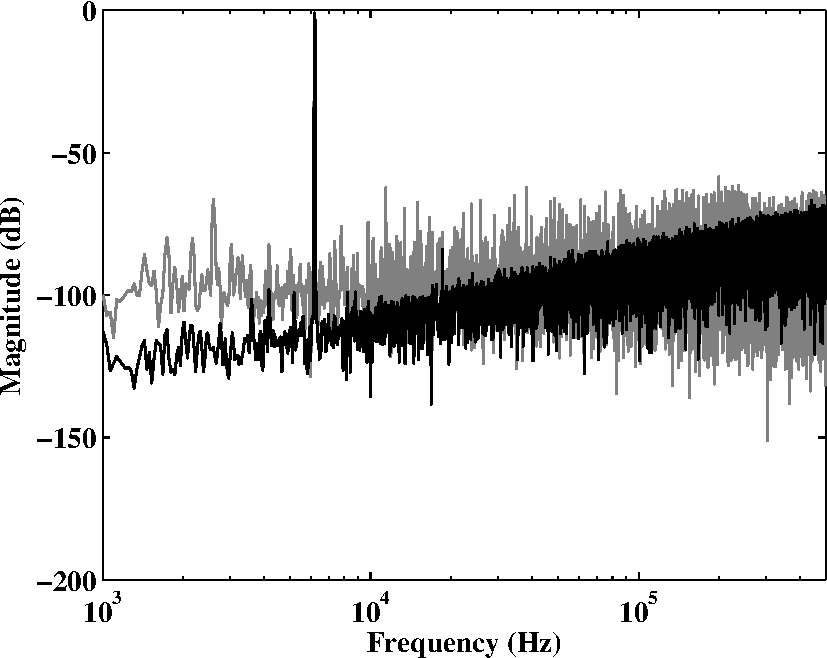
\includegraphics[width=\myfigwidth]{graphics/olsdmspice}}
 \caption{FFT of output from first order OLSDM simulation in SPICE.}
 \label{p4fig:olsdmspice}
\end{figure}

 \begin{figure}[htbp] 
\centerline{ 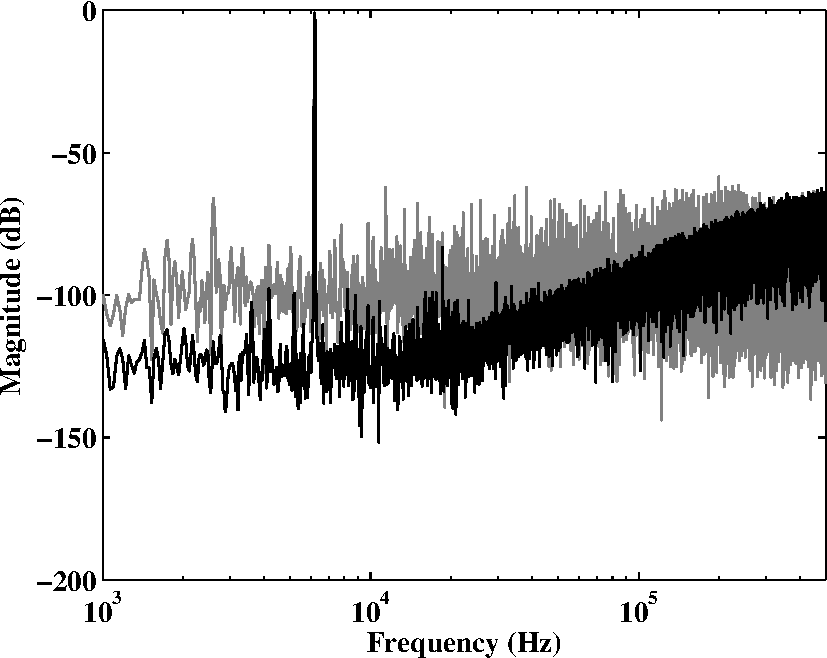
\includegraphics[width=\myfigwidth]{graphics/olsdmspice2}}
 \caption{FFT of output from second order OLSDM simulation in SPICE.}
 \label{p4fig:olsdmspice2}
\end{figure}


%-------------------------------------------------------
\section{Future Work}
%-------------------------------------------------------
There are no integrated circuit implementations of an amplitude
modulated OLSDM as of
yet. An integrated circuit implementation would be the next step. It
is needed to check whether the amplitude modulated OLSDM has a place in the
family of analog-to-digital converters, or whether it is just of
academic interest. There are many questions to be 
answered and some questions that have not yet been asked. The
switched capacitor analog modulo integrator is, to our knowledge, new 
circuit, and it may find applications outside the realm of OLSDM.  
 
%-------------------------------------------------------
\section{Conclusion}
%-------------------------------------------------------
We introduced the switched capacitor analog modulo integrator, which
to our knowledge is a new circuit. We introduced
the amplitude modulated open loop \SD modulator (OLSDM), which is an analog modulo integrator
followed by a quantizer and a modulo differentiator. The mathematical
equivalence between low pass \SD modulators and OLSDM was
explained. Behavioral simulations confirmed the equivalence. The
necessary circuit, a switched capacitor analog modulo integrator, was explained in detail. 
Behavioral level simulations in SPICE of the analog modulo
integrator verified the function, and proved the concept of
amplitude modulated OLSDM.

%------------------------------------------------------------------------
%\begin{acknowledgements}
%------------------------------------------------------------------------
\section*{Acknowledgments}
 Financial support from the Norwegian Research Council through the
project Smart Microsystems for Diagnostic Imaging in Medicine (project
number 159559/130) and the project ASICs for Microsystems (project
number 133952/420) is gratefully acknowledged.
%\end{acknowledgements}




%\bibliography{IEEEabrv,wulff}

% \begin{thebibliography}{00}

% \bibitem{Widrow56}
% Widrow, B.: 1956, `A Study of Rough Amplitude Quantization by Means of Nyquist
%   Sampling Theory'.
% \newblock {\em Circuit Theory, IRE Transactions on} {\bf 3}(4), 266--276.

% \bibitem{claasen80}
% Claasen, T. A. C.~M., W.~F.~G. Mecklenbraucker, J.~B.~H. Peek, and N. van
%   Hurck: 1980, `Signal Processing Method for Improving the Dynamic Range of A/D
%   and D/A Converters'.
% \newblock {\em {IEEE} Trans. Acoust., Speech, Signal Processing} {\bf 28}(5),
%   529--538.


% \bibitem{hovin97}
% H{\o}vin, M., A. Olsen, T.~S. Lande, and C. Toumazou: 1997, `Delta-Sigma
%   Modulators Using Frequency -Modulated Intermediate Values'.
% \newblock {\em {IEEE} J. Solid-State Circuits} {\bf 32}(1), 13--22.

% \bibitem{wismar06}
% Wismar, U., D. Wisland, and P. Anderiani: 2006, `A 0.2V 0.44 �W 20 kHz Analog
%   to Digital Modulator with 57 fJ/conversion FoM'.
% \newblock In: {\em Proc ESSIRC'06}, Vol.~1. pp. 187--190.


% \bibitem{wisland02}
% Wisland, D.~T., M.~E. H{\o}vin, L.~A. Fleischer, and T.~S. Lande: 2002a, `A new
%   scalable non-feedback sigma-delta Digital-to-Analog Converter'.
% \newblock In: {\em Proc. ICECS'02}, Vol.~1. pp. 331--334.

% \bibitem{brooks97}
% Brooks, T.~L., D.~H. Robertson, D.~F. Kelly, A.~D. Muro, and S.~W. Harston:
%   1997, `A Cascaded Sigma-Delta Pipeline A/D Converter with 1.25MHz Signal
%   Bandwidth and 89 dB SNR'.
% \newblock {\em {IEEE} J. Solid-State Circuits} {\bf 32}(12), 1896--1906.


% \bibitem{johns}
% Johns, D. and K. Martin: 1997, {\em Analog Integrated Circuit Design}.
% \newblock John Wiley \& Sons, Inc.



% \bibitem{IEEE-1241}
% IEEE: 2001, `IEEE standard for terminology and test methods for
%   analog-to-digital converters'.
% \newblock IEEE Std 1241-2000.


% \bibitem{wisland02a}
% Wisland, D.~T., M.~E. H{\o}vin, L.~A. Fleischer, and T.~S. Lande: 2002b, `A
%   second-order non-feedback /spl Delta//spl Sigma/ modulator for D/A
%   conversion'.
% \newblock In: {\em Proc. ICECS'02}, Vol.~1. pp. 327--330.


% \end{thebibliography}

%\input{authors.tex}

%\begin{vitae}



%\centerline{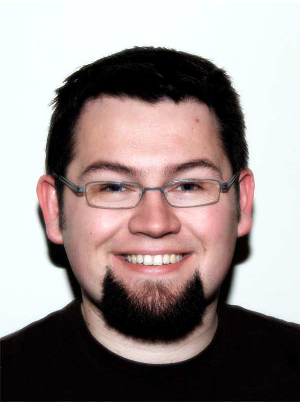
\includegraphics[width=20mm]{wulff-photo} }
%\Vauthor{Carsten Wulff}
%\begin{figure}[h]

%\end{figure}
% \textbf{Carsten Wulff}
%%received the M.Sc degree in electrical engineering from the Department
%of Physical Electronics, Norwegian University of Science and
%Technology (NTNU), in 2002. He was employed as a research assistant
%at NTNU during 2003-2004. Since 2004 he has been working towards his PhD. In
%2006-2007 he was a visiting researcher at Department of Electrical and
%Computer Engineering, University of Toronto. 
% His present research interest include analog and mixed-signal
%CMOS design, and design of analog-to-digital converters with a
%particular focus on comparator based switched capacitor circuits.   

%\Vauthor{{\O}ystein Knauserud}
%\textbf{{\O}ystein Knauserud}
%received the M.Sc degree in electrical engineering from the Department of Electronics and Telecommunication, Norwegian University of Science and Technology (NTNU), in 2006. He is currently at ARM, Embedded Graphics Solutions in Trondheim, Norway.


%\begin{figure}[h]
%\centerline{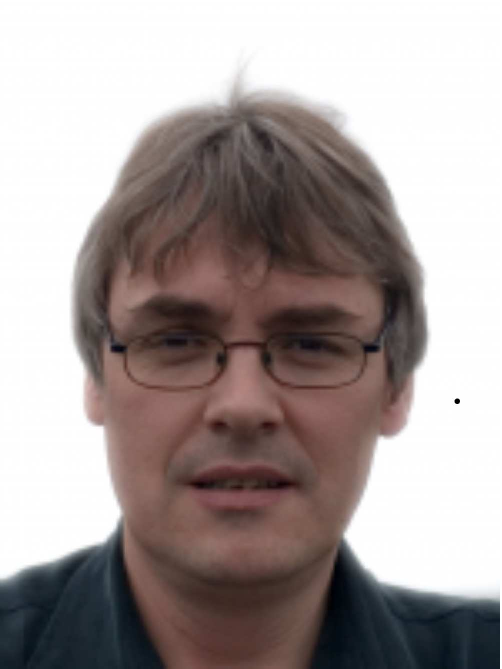
\includegraphics[width=20mm]{trond} }
%\end{figure}

%\textbf{Trond Ytterdal}
%\Vauthor{Trond Ytterdal}
%received his M.Sc. and Ph.D. degrees in electrical
%engineering from the Norwegian Institute of Technology in 1990 and 1995,
%respectively. He was employed as a research associate at the Department of
%Electrical Engineering, University of Virginia (1995-1996) and as a research
%scientist at the Electrical, Computer and Systems Engineering Department,
%Rensselaer Polytechnic Institute in Troy, New York (1996-1997). From 1997 to
%2001 he worked as a senior ASIC designer at Nordic Semiconductor in
%Trondheim, Norway. In 2001 he became a Professor at the Department of
%Electronics and Telecommunication, Norwegian University of Science and
%Technology (NTNU). Prof. Ytterdal's present research interests include
%design of analog integrated circuits, behavioral modeling and simulation of
%mixed-signal systems, modeling of nanoscale transistors and novel device
%structures for application in circuit simulators. He has published more than
%100 scientific papers in international journals and conference proceedings.
%He is a co-author of the books Semiconductor Device Modeling for VLSI
%(Prentice Hall, 1993), Introduction to Device Modeling and Circuit
%Simulation (Wiley, 1998) and Device Modeling for Analog and RF CMOS Circuit
%Design (Wiley, 2003), and has been a contributor to several other books
%published internationally. He is also a co-developer of the circuit
%simulator AIM-Spice. Prof. Ytterdal is a member of The Norwegian Academy of
%Technological Sciences and a Senior Member of IEEE.




%\end{vitae}


%\end{document}

\renewcommand{\figurename}{Fig.}
\renewcommand{\myfignamehead}{Fig.}
\chapter{Paper 3}\label{sc:p3}
\textbf{\Large Resonators In Open-Loop Sigma-Delta Modulators}\\
\indent Carsten Wulff and Trond Ytterdal\\
\indent Submitted to IEEE Transactions on Circuits and Systems I: Regular papers\\
%\def\abstract{\section{Abstract}}
\renewcommand\myfigname{sdrfig:}
\renewcommand\myeqname{sdreq:}
%\renewcommand{\appendices}{}
%\newcommand{\myappname}{Section}
\newcommand{\myappname}{Section }
\newcommand{\myappendices}{}

%\newcommand{\myintmodref}{}
\newcommand{\mymodintfig}{
 \begin{figure}[htbp]
   \centering{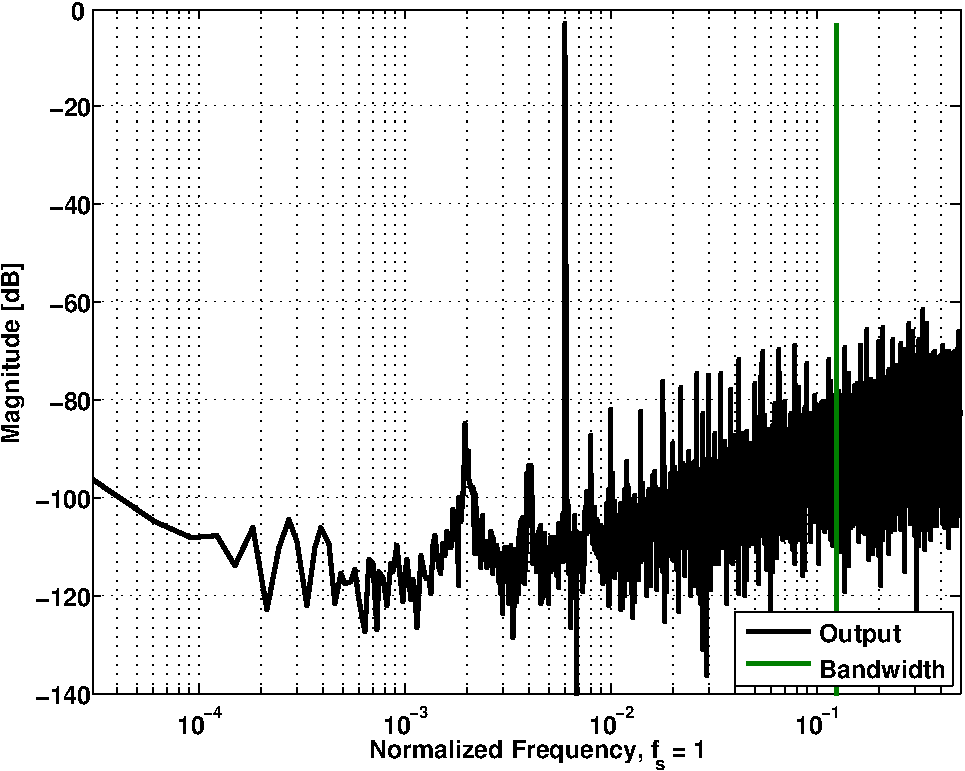
\includegraphics[width=\myfigwidth]{graphics/intmod_z}}
   \caption{SIMULINK model, SNDR = 52.20-dB}
   \label{sdrfig:intmod_z} 
 \end{figure}

 \begin{figure}[htbp]
   \centering{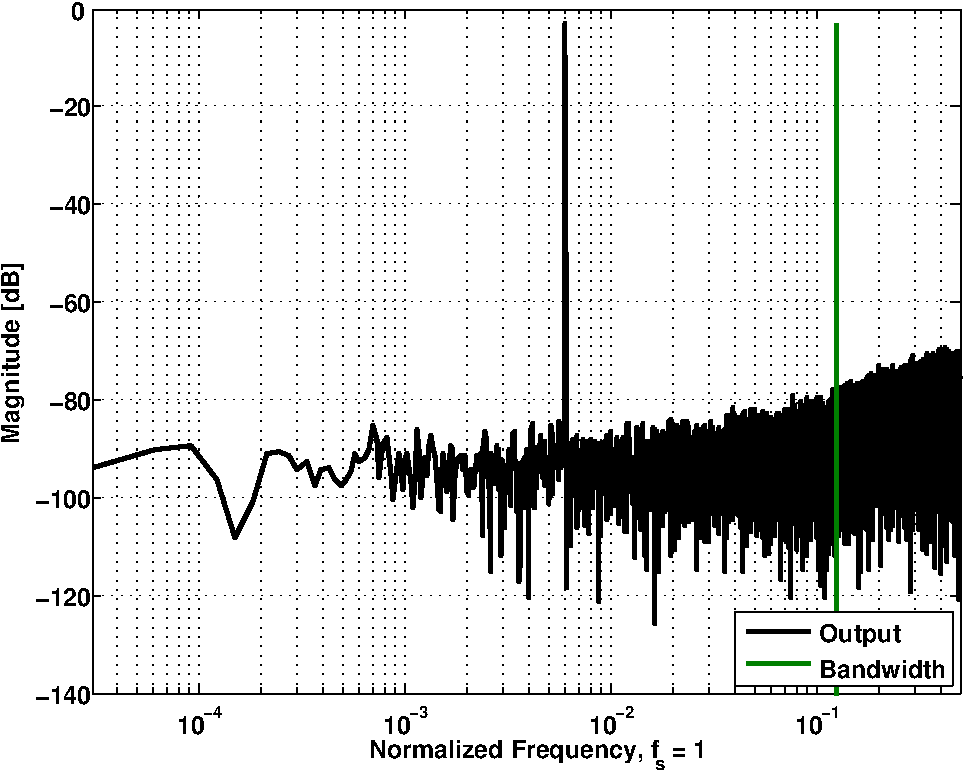
\includegraphics[width=\myfigwidth]{graphics/intmod_d}}
\caption{Approximation, SNDR = 51.44-dB}
\label{sdrfig:intmod_d}
\end{figure}

\begin{figure}[htbp]
\centering{ 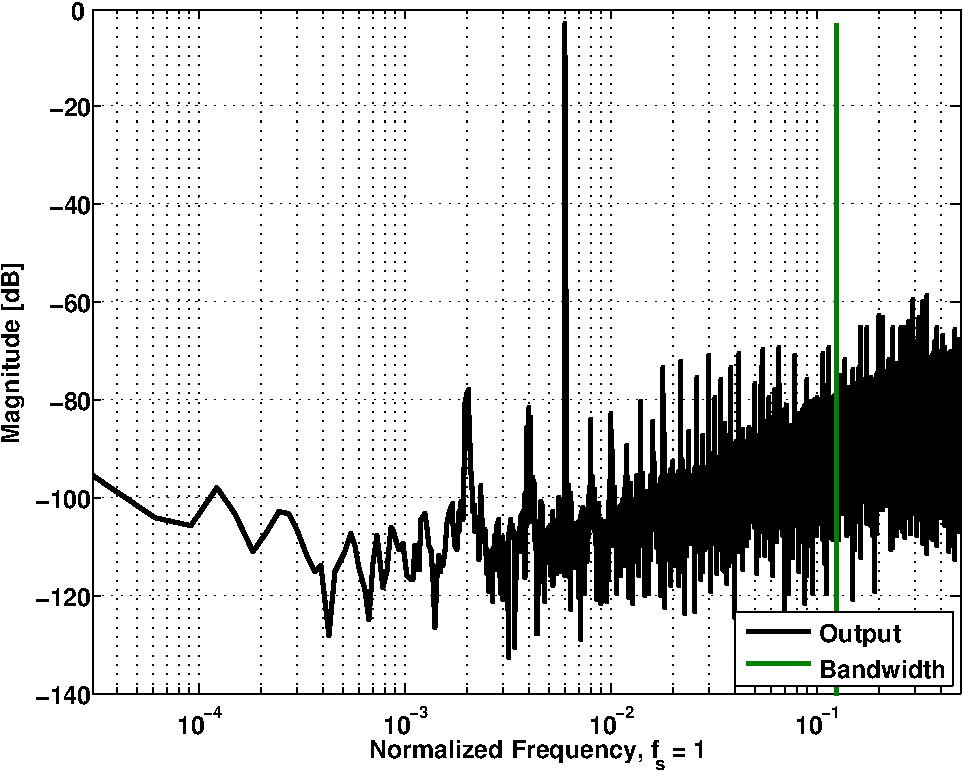
\includegraphics[width=\myfigwidth]{graphics/intmod_spice}}
\caption{SPICE model, SNDR = 51.66-dB}
\label{sdrfig:intmod_spice}
\end{figure}

\begin{figure}[htbp]
\centering{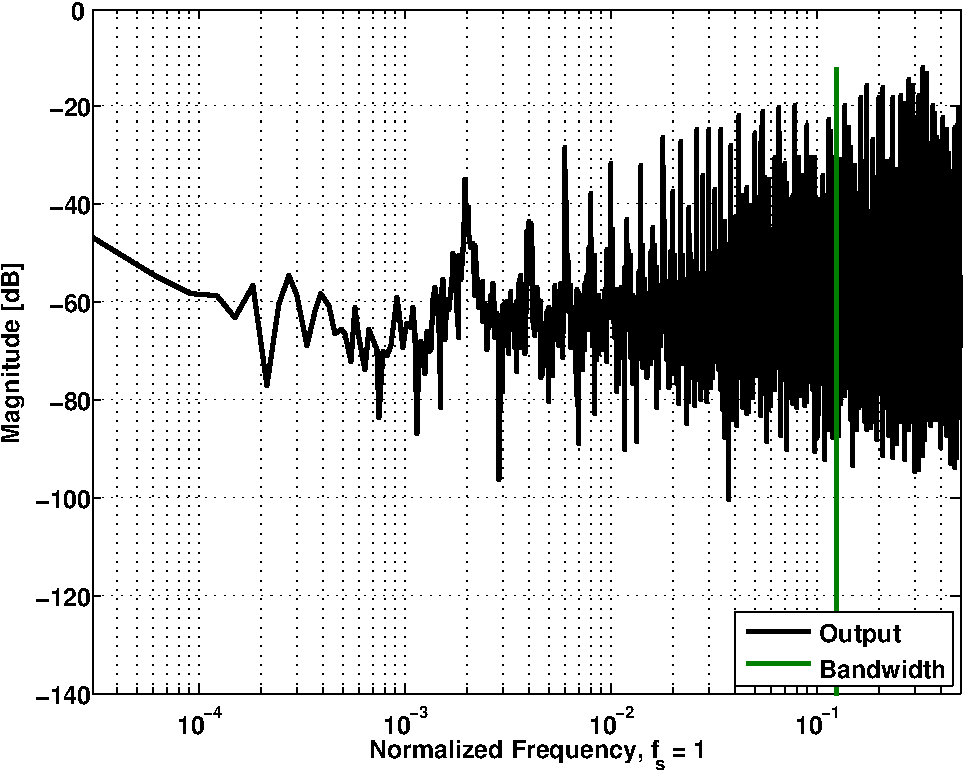
\includegraphics[width=\myfigwidth]{graphics/intmod_u}}
 \caption{FFT of $u_n$}
\label{sdrfig:intmod_u} 
\end{figure}

}

\section*{Errata}
We recieved a response to this paper quite quickly, and all
reviewers found the paper interesting, but wanted more information. We
were asked to submit a new version for review with the following
changes. 
\begin{itemize}
\item Discuss the effects of mismatch in capacitors
\item Discuss why adding zeros at non-zero frequency is better than at
  zero frequency
\item Add more introduction to OLSDM and SDM
\item Discuss the effects of offset errors in comparators
\end{itemize}
These changes have been included in the paper below.




\newcommand{\simulink}{Simulink  }
\newcommand{\matlab}{MATLAB }
%\CWabstract{
%\section*{Abstract}
%########################################################################
%\begin{quote}
%{\center\textbf{Abstract:}}\\
\begin{abstract}
In this paper we introduce the modulo resonator for use in \textit{open-loop
sigma-delta modulators} (OLSDM). The OLSDM presented in this work is
intended for use in high accuracy (14-bit), high-speed analog-to-digital
converters.

The modulo resonator is used with a modulo notch filter to
insert a zero in the noise transfer function at a non-zero
frequency. 
The effect of finite gain in modulo integrators and modulo resonators
are described and verified through simulation. 
The modulo resonator and previously published modulo
integrator are used in a behavioral model of a switched-capacitor fifth-order OLSDM with more
than 13-bit effective number of bits for an oversampling ratio of
four. We prove for
the N-order OLSDM that the number of bits in the quantizer (B) must be
larger than N to ensure equivalence between OLSDM and sigma-delta
modulation.
\end{abstract}
%\end{quote}
%}

\begin{keywords}
%\keywords{ 
Sigma-delta modulators, switched-capacitor circuits, modulo
integrator, modulo resonator, open-loop sigma-delta modulators
\end{keywords}

%########################################################################
\section{Introduction}
%########################################################################
If one wants to make an analog-to-digital converter with high
resolution ($>$12-bit) a sigma-delta modulator is a natural choice. 
Sigma-delta modulators are prevalent as analog-to-digital converters in applications with low to medium
bandwidth  ($<$ 10MS/s) and high resolution.  
The sigma-delta modulator trades speed for resolution.
It typically uses a low-resolution quantizer ($<$
6-bit) with a large quantization error. The quantizer is run at a
higher speed than required by the system bandwidth. By using clever
analog-filters and feedback techniques the in-band quantization error can be
lowered, while the out-of-band quantization error can be large. This
out-of-band quantization error is easily filtered using digital
filters. 

The family of sigma-delta modulators is large, with
many diverse family members. One of the oldest members is the low-pass
sigma-delta modulator, which in its simplest form consists of an
integrator followed by a quantizer. The quantized signal is fed-back
to the input through a digital-to-analog converter (DAC) and subtracted from
the input. The transfer function of the modulator is different for the
input signal and the quantization noise.\footnote{This assumes a linear model of the quantizer,
  since the transfer function is only defined for a linear system} The input
signal will undergo an integration followed by a
differentiation and have a transfer function of one. The quantization noise will be
differentiated and thus high pass filtered. 

In an ideal world, with no voltage swing limitations, a low-pass
sigma-delta modulator
could be implemented by an integrator 
followed by a quantizer and a differentiator, but since supply voltage
is limited in electronic circuits, and an integrator  
has infinite DC gain, it is difficult to implement. Somehow
the output swing of the integrator has to be limited. Feedback is
typically used to limit the output swing of the integrator. 
 
In this
paper we discuss a small sub group that we denote Open-loop sigma-delta
modulators (OLSDM).  We define OLSDM as \textit{any sigma-delta modulator that does
not have feedback of the quantized modulator output signal}. 

The idea of a open-loop sigma-delta modulator is to use a limiting
function (for example a modulo) to limit the signal swing in the
analog domain, replacing the feedback of the quantized signal. After
quantization  the inverse limiting function is used to reverse the
effects of the limit in the analog domain. This idea is
by no means new. One of the first suggestion of an OLSDM was almost thirty years ago in
\cite{claasen80}. Although there was no system 
implementation they explained a method that avoided feedback of the
quantized signal. Little over a decade ago the  Frequency
Sigma-Delta Modulator (FSDM) \cite{hovin97.2} was presented, and more
recently \cite{wismar07a}. 
In the FSDM a voltage controlled
oscillator (VCO) is used as the modulo integrator, and it was shown in \cite{hovin97.2} that the pre-processing
in FSDM is equivalent to modulo integration. 
The
non-feedback \SD digital-to-analog modulator, where the
integrator is implemented as a digital modulo integrator, was
described in \cite{wisland03a}. 
In \cite{wulff08a} an amplitude modulated switched-capacitor open-loop
sigma-delta modulator was introduced. A switched-capacitor 
modulo integrator was used to perform the modulo integration.

An example of analog-to-digital conversion with open-loop sigma-delta
modulation is shown in Fig.
\ref{sdrfig:olsdm-basic}. The input
signal, $x$, is accumulated by the integrator ($\langle\Sigma\rangle$). The
integrator in Fig. \ref{sdrfig:olsdm-basic} is a modulo integrator that
wraps around when the sum exceeds the
range ($R$). The output of the integrator ($u$) is quantized by a quantizer,
which is modeled as a linear addition of
quantization noise ($q$). The conditions  for modeling a
quantizer as linear addition of noise was covered in 
\cite{widrow56}. The modulo differentiator ($\langle\Delta\rangle$) reverse the effect
of the modulo
integrator. The decimation filter required to down-sample the output of
the modulator is not shown. 

In this modulator the input signal passes through unchanged. The quantization noise pass through the
differentiator and is first order high-pass filtered. 

The sigma-delta modulator in Fig. \ref{sdrfig:olsdm-basic} is equivalent
to a first order
low-pass sigma-delta modulator providing certain conditions are met.

\begin{figure}[htbp]
\centerline{ 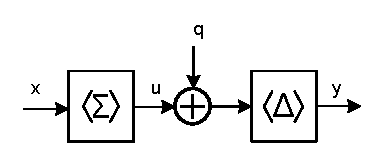
\includegraphics[width=\myfigwidthb]{graphics/osd}}
  \caption{First order low-pass open-loop sigma-delta modulator}
  \label{sdrfig:olsdm-basic}
\end{figure}

The application envisioned for the  OLSDM discussed in this paper is as a front-end in a high
speed ($>$10MS/s), high resolution (14-bit)  analog-to-digital converter. The advantage of OLSDM is that
it is trivial to use high-latency quantizers since there is no feedback of the quantized
modulator output. 

There are two unsolved challenges that this paper discuss: when is
open-loop sigma delta modulation equivalent to sigma-delta modulation,
and how to introduce zeros in the noise transfer function (NTF) at non-zero
frequencies. 

%-------------------------------------------------------
\subsection{When is OLSDM equivalent to SDM?}
%-------------------------------------------------------
It is observed in simulation that open-loop sigma-delta
modulation (OLSDM) is not always equal to
sigma-delta modulation (SDM). Whether an OLSDM works as an SDM depends
on the input signal amplitude and the number of bits in the
quantizer. The input signal amplitude must be less than $|x_n| < R/2$
(0dBFS\footnote{0dB referred to full scale amplitude, $R/2$}), but OLSDM sometimes
loose its noise shaping at less than 0dBFS. 

In \cite{wulff08a} an error
correction scheme was used to restore the noise shaping for input
signal amplitudes up to 0dBFS. But the error correction assumed that
the input frequency was much less than the sampling frequency ($f_i << f_s$). For some applications (like high speed, high
resolution) the OSR can be low ($OSR < 8$) and $f_i << f_s$ is no
longer valid. 

The number of bits in the quantizer affect the equivalence
between OLSDM and SDM. It is observed that the number of bits in
the quantizer must be larger than the order of the modulator. This was
proved for the special case of a second order OLSDM in
\cite{wisland02a}.

We will prove for
the N-order OLSDM that the number of bits in the quantizer (B) must be
larger than the order (N) to ensure equivalence between OLSDM and SDM.

\subsection{Zeros in NTF at non-zero frequency}
Previous OLSDMs have all been low order low-pass sigma-delta
modulators. Low order low-pass sigma-delta modulators are unsuited for high
conversion rate applications due to the high oversampling ratio
required to get high resolution, assuming a low resolution quantizer
is used. 

If the sampling frequency ($f_s$) is constant, the resolution can be increased by
adding more zeros to the noise transfer function (NTF). Adding zeros at a non-zero
frequency ($\omega_0 > 0$) reduce the OSR more than adding them at
zero frequency. To see why zeros at a non-zero frequency reduce the
OSR more than adding them at zero frequency it is instructive to look at a
graphical comparison. In \reg{f0zerof1} a comparison between two
fifth-order sigma-delta modulators is shown, one with all zeros at
zero-frequency (dashed line) and one modulator with one zero at
zero-frequency and two complex conjugate zeros at non-zero frequencies
(solid line). Since the noise
transfer function is real the zeros must be complex conjugate, thus to
get two zeros at non-zero frequency we need four zeros, two at
positive frequencies and two at negative frequencies. The dominating
contribution from the noise transfer functions will be at high
frequencies. So although the NTF with non-zero frequency zeros has less
attenuation at low frequencies it has more attenuation at high
frequencies (for example at a normalized frequency of 0.1 the
difference is almost 20dB). Accordingly, for an oversampling ratio of
four (marked by the dotted line), the NTF with zeros at a non-zero
frequency has more attenuation, and as a consequence yields a higher
resolution for a given OSR.

\begin{figure}[htbp]
\centerline{ 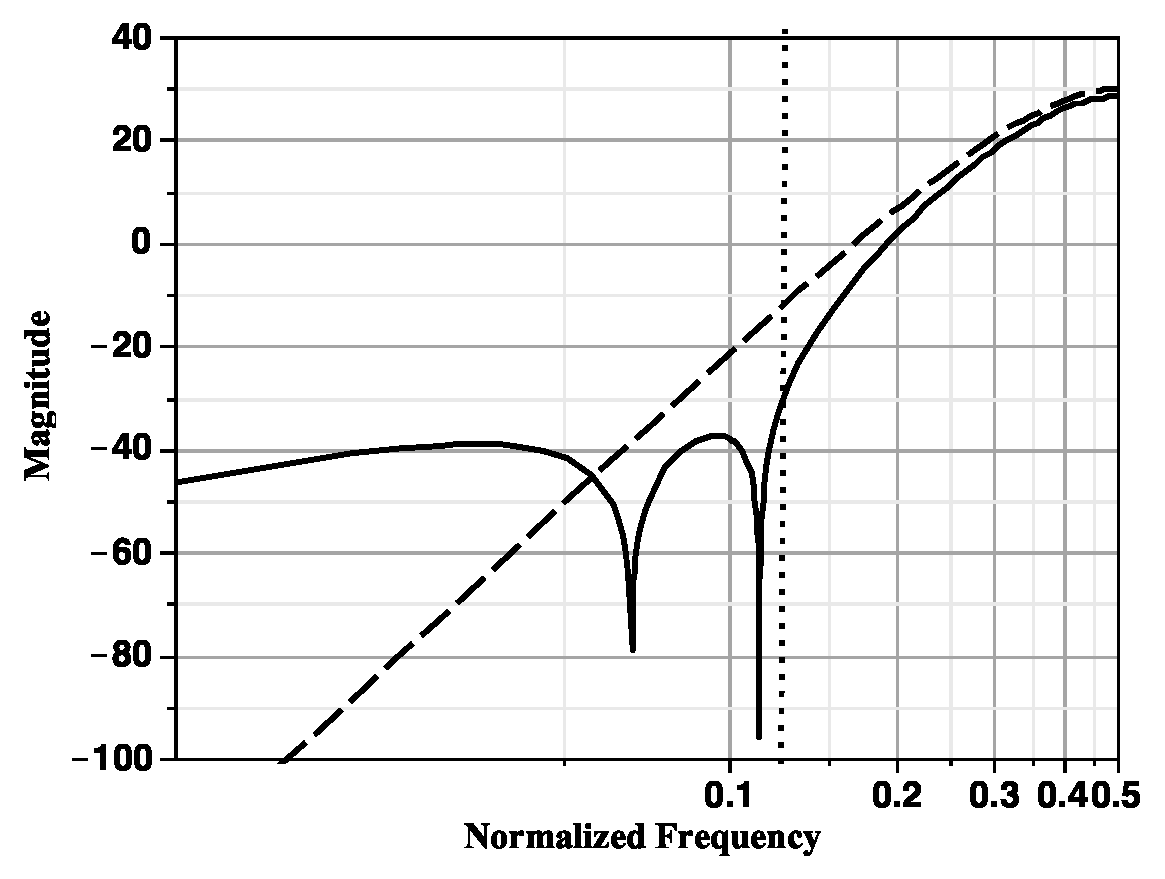
\includegraphics[width=\myfigwidth]{graphics/f0zerof1}}
  \caption{Comparison between a fifth-order sigma-delta modulator with
  all zeros at zero frequency (dashed-line) and fifth-order
  sigma-delta modulator with one zero at zero
  frequency and two complex conjugate zeros at optimum frequencies.}
  \label{sdrfig:f0zerof1}
\end{figure}


To the best of our
knowledge, zeros at non-zero frequencies have not been used in OLSDM
before this work. 

The paper is organized as follows: In Section \ref{sdrbasicmodulo} 
OLSDM is explained and requirements for input signal amplitude and quantizer bits are
derived. In Section \ref{sdrmodulointegrators} the key component of OLSDM, the
modulo integrator, is described in detail, including the effects of
finite gain in modulo integrators. The modulo integrator has
previously been described in \cite{wulff08a}, but the effects of
finite gain in modulo integrators has not been exhaustively covered.

The modulo resonator is introduced in
Section \ref{sdrmoduloresonator}. The modulo integrator and modulo
resonator are combined in Section \ref{sdrmatlabsim} to make a behavioral
model of a fifth
order low-pass OLSDM with more than 13-bit effective number of bits with an
OSR of four. Simulation results from behavioral level models in \matlab \cite{matlab}
and SPICE are presented in Section \ref{sdrmatlabsim}.


%########################################################################
\section{When is OLSDM equivalent to SDM?}\label{sdrbasicmodulo}
%########################################################################
The modulo operator is used extensively in OLSDM to limit the signal
swing at the output of modulo integrator. The modulo operator is written as
\eqn{
\label{sdreq:modulo}
  x_r = \langle x \rangle_R
}
where $x \in \langle -\infty,\infty \rangle $ is the input signal, $R$ is the range and
$x_r  \in \langle - R/2, R/2 \rangle$ is the residue after dividing by
the range, $R$. 
This
modulo function is not the normal mathematical modulo function, but
a
function that computes the remainder of the input signal after
rounding it to an integer number of full scale signal swings ($R$).

The modulo is similar 
to what was used in \cite{lipshitz07} where they proved the
equivalence of the  open-loop and closed loop representations by
symbolic manipulation. The modulo arithmetic used in OLSDM has  previously been used in
comb filters, as was
shown in \cite{chu84}. 
%The discrete time equations for OLSDM will be derived, and from
%these it will be shown that a open-loop sigma-delta modulator is equivalent
%to a sigma-delta modulator, provided certain conditions of the input signal amplitude
%and the quantizer bits are met.

The following theorem is useful for the derivations below.
\begin{theorem}
The modulo of the sum of modulo is equal to the modulo of sum if the range of the
two modulus are equal, $R_0 = R_1=R$
\eqn{
\label{sdreq:prop1}
\langle \langle x \rangle_{R_0} + \langle y \rangle_{R_0} \rangle_{R_1} = \langle
  x + y \rangle_R
}
\end{theorem}
A proof of the theorem is included in \myappname \ref{sdrap:modproof}

The modulo integration, shown in Fig \ref{sdrfig:olsdm-basic}, is
written as
\eqn{
\label{sdreq:modint}
  u_n = \left\langle\sum_{i=0}^\infty{x_{n-i-1}}\right\rangle_R
}
where $x_n$ is the input signal to the integrator at time $n$, $u_n$ is the
modulator output signal, and $n$ is the discrete time step. The input signal at
time $n-1$ is written as $x_{n-1}$.

The output of the modulator in Fig. \ref{sdrfig:olsdm-basic}
is
\eqn{
\label{sdreq:modout}
  y_n = \left\langle u_n - u_{n-1} + q_n - q_{n-1}\right\rangle_R
}
where $q_n$ is the quantization noise. 

Insert \req{modint} in
\req{modout} and let $e_n = q_n - q_{n-1}$

\eqn{
\label{sdreq:modout1}
  y_n = \left\langle \left
      \langle\sum_{i=0}^\infty{x_{n-i-1}}\right\rangle_R -
    \left\langle\sum_{i=0}^\infty{x_{n-i-2}}\right\rangle_R  + e_n \right\rangle_R
}
With \req{prop1}  \req{modout1} reduces to
\eqn{ 
\label{sdreq:modout3}
  y_n = \left\langle x_{n-1} + e_n \right\rangle_R
}
The discrete time equation for a first order low-pass sigma-delta
modulator is
\eqn{
\label{sdreq:sdm}
  y_n  = x_{n-1} + q_n - q_{n-1}
}
Equation \req{modout3} is equal to \req{sdm} if 
\eqn{
  | x_n  + e_n| < R/2
}

The absolute value of the filtered quantization noise ($|e_n|$) has a
maximum value of one LSB (Least
Significant Bit), since $|q_n| \leq 1/2 LSB$ and $e_n = q_n -
q_{n-1}$. Here $LSB = R/2^B$, where $B$ is the number of 
bits in the quantizer. 

The input signal for first order open-loop
sigma-delta modulator must be limited by 
\eqn{
\label{sdreq:modlimit}
  |x_n| < R/2 - 1 LSB = R( 1/2 -1/2^B)
}
%Equation \req{modlimit} clearly shows that quantizers with few bits
%are unsuited for OLSDM, since they would place severe limitations on
%the input signal. 
We will derive the general input signal limitations for N-order OLSDM,
but to reduce the length of equations we define
\eqn{
  f_{x,n} = \sum_{i=0}^\infty{x_{n-i}}
}
and from \req{prop1}
\eqn{
\label{sdreq:fdef1}
  \left\langle \langle f_{x,n} \rangle_R  - \langle f_{x,n-1} \rangle_R
  + e_n \right \rangle_R = \langle x_n +e_n \rangle_R
}

For second order OLSDM (Fig. \ref{sdrfig:mod2}) the
output of the first integrator is
\eqn{
  u_n = \langle f_{x,n-1} \rangle_R      
}
and the output of the second integrator is
\eqn{
  u_{1,n} = \langle f_{u,n-1} \rangle_R
}

\begin{figure}[htbp]
\centerline{ 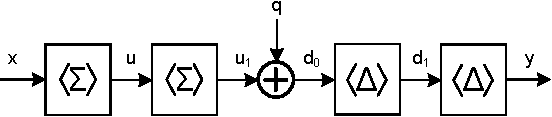
\includegraphics[width=\myfigwidth]{graphics/osd2}}
  \caption{Second order low-pass open-loop sigma-delta modulator}
  \label{sdrfig:mod2}
\end{figure}

The quantized signal is 
\eqn{
  d_{0,n} = \langle f_{u,n-1} \rangle_R + q_n
}
And the output signal of the first modulo differentiator is
\eqn{
  d_{1,n} = \left\langle \langle f_{u,n-1} \rangle_R - \langle f_{u,n-2}
    \rangle_R +e_n\right\rangle_R
}
which by \req{fdef1} is written as
\eqn{
  d_{1,n} = \langle u_{n-1} + e_n \rangle_R
}
The output signal of the modulator is
\eqn{
y_n = \left \langle \langle f_{x,n-1} \rangle_R - \langle f_{x,n-2}
  \rangle_R + e_n - e_{n-1} \right\rangle_R
}
which by \req{fdef1} is
\eqn{
\label{sdreq:modout2}
y_n = \left \langle x_{n-1}  + q_n - 2 q_{n-1} + q_{n-2} \right\rangle_R
}

The maximum absolute
value of the quantization noise in 
\req{modout2} is 
\eqn{|q_n| + |2q_{n-1}| + |q_{n-2}| = 1/2 + 1 +1/2 =
2
}
From this it follows that the input signal must be limited by
\eqn{
\label{sdreq:lim2}
  |x_n| < R/2 - 2 LSB = R(1/2 - 2/2^B)
}
\req{lim2} is sufficient to ensure that the second order
OLSDM is equivalent to a second order SDM. It can be shown that for third
order OLSDM the requirement is  
\eqn{
  |x_n| < R/2 - 4 LSB = R(1/2 - 4/2^B)
}
For N-order OLSDM the input signal must be limited by
\eqn{
\label{sdreq:inlimit}
  |x_n| < R(1/2 - 2^{N-1}/2^B)
}
If $B=N$ the input signal limit is not practical since
\eqn{
  |x_n| < R(1/2 - 2^{N-1}/2^B) = R(1/2-1/2) = 0
}
Accordingly, $B > N$ to ensure that N-order OLSDM is equivalent to
N-order SDM. This is equivalent to the quantizer 
non-overload criteria in SDM proved in
\cite{lokken06}. An N-order sigma-delta modulator will not overload
the quantizer if the input signal is limited by
$|x_n| < R/4$, and $B=N+1$. 

For $B=N+1$ in \req{inlimit}
\eqn{
  |x_n| < R(1/2 - 1/4) = R/4
}

In the next section we will cover the key component of
analog-to-digital OLSDM, the modulo integrator.



%########################################################################
\section{Modulo integrator}\label{sdrmodulointegrators}
%########################################################################

In this section we discuss the implementation of a
modulo integrator in behavioral level models, the switched-capacitor
implementation, and effects of finite opamp gain in the modulo integrator. 

%-------------------------------------------------------
\subsection{Behavior level implementation}
%-------------------------------------------------------
The output of the modulo integrator is described by 
\eqn{
\label{sdreq:modint_copy}
  u_n = \left\langle\sum_{i=0}^\infty{x_{n-i-1}}\right\rangle_R
}
In behavioral level models \req{modint_copy} is impractical 
due to the infinite modulo. In the definition of the
modulo \req{modulo}  the input signal can take any value,
$x_n \in \langle-\infty,\infty\rangle$. This requires the modulo
integrator to wrap around infinitely many times if the output signal
is to be limited by $u_n \in \langle -R/2, R/2\rangle$. But since the
input signal is limited by \req{inlimit}, the infinite modulo is
unnecessary. Assume that $|x_n| < R/2$, which by
\req{inlimit} must be true, then the maximum value after integration
,but before the modulo, is limited by $u_{before,n} \in \langle -R, R
\rangle$. Fig. \ref{sdrfig:modint} shows an example of the output
($u_{before,n}$) before modulo, and after modulo ($u_n$) for a sinusoidal
input signal ($x_n$). The modulo integrator is implemented by adding or
subtracting the range $R$.
\begin{figure}[htbp]
\centerline{ 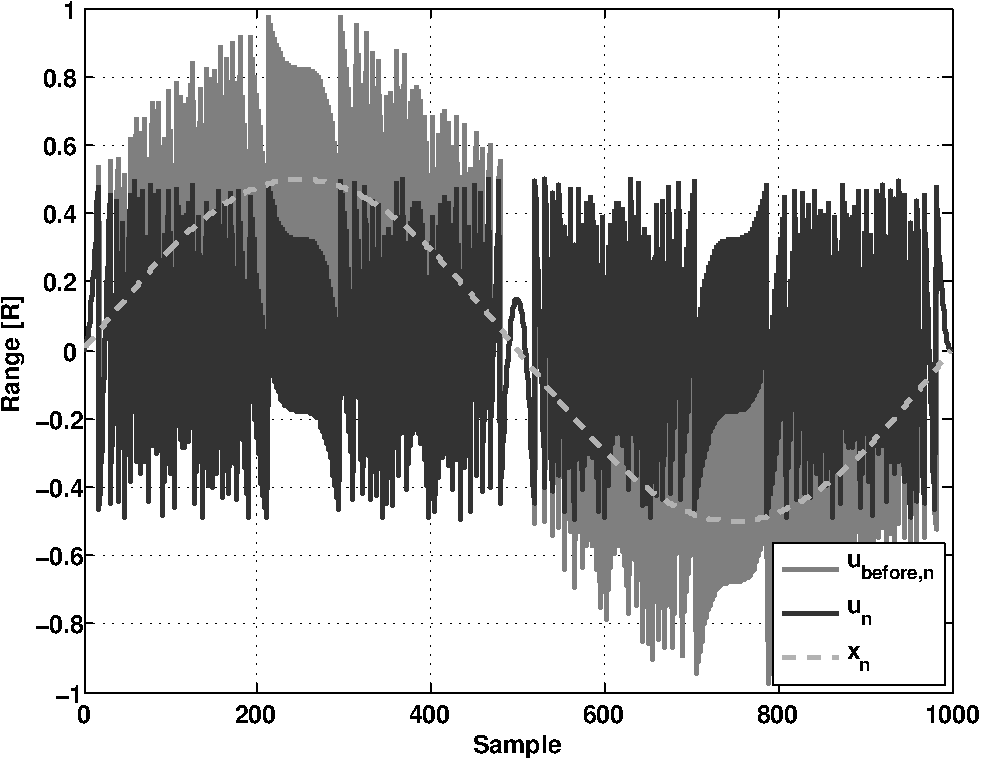
\includegraphics[width=\myfigwidth]{graphics/modint_res}}
  \caption{States of the modulo integrator for a sinusoidal input
    $x_n$. The output before modulo is $u_{before,n}$ and the output
    after is $u_n$.}
  \label{sdrfig:modint}
\end{figure}
The modulo operation can now be defined as
\eqn{
  u_{before,n} = u_{n-1} + x_{n-1}
}
and 
\begin{numcases}{u_n = }
\label{sdreq:modintdef}
u_{before,n} + R & $u_{before,n} \in \langle -R, -R/2 ]$\nonumber\\ 
u_{before,n}  & $u_{before,n} \in \langle -R/2 , R/2 \rangle$ \nonumber\\
u_{before,n} - R & $u_{before,n} \in [ R/2, R \rangle$
\end{numcases}
%or written as \req{modulo}
%\eqn{
%\label{sdreq:limmodulo}
%  x_r = \langle x \rangle_R,\: x \in \langle -R,R  \rangle, \: x_r \in
%  \langle -R/2,R/2 \rangle
%}


The modulo integrator described by \req{modintdef} can be implemented
as a switched-capacitor (SC) circuit \cite{wulff08a}. 

%-------------------------------------------------------
\subsection{Switched-capacitor modulo integrator}\label{sdrSscmod}
%-------------------------------------------------------
The SC modulo integrator is based on the
parasitic insensitive integrator shown in Fig. \ref{sdrfig:scint}. The
input signal is sampled at the end of $p_1$. In $p_2$ the charge of
$C_1$ is moved to $C_2$ by forcing node $V_x$ equal to zero
with the opamp.
\begin{figure}[htbp]
\centerline{ 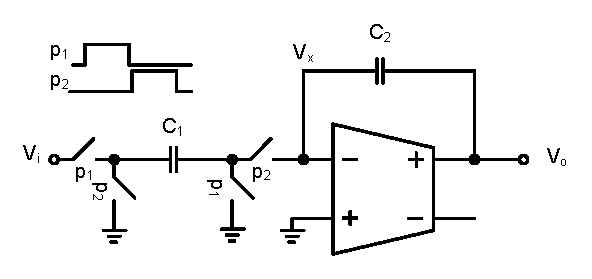
\includegraphics[width=\myfigwidth]{graphics/sc_int}}
  \caption{Parasitic insensitive switched-capacitor integrator}
  \label{sdrfig:scint}
\end{figure}
The switched-capacitor modulo integrator is shown in
Fig. \ref{sdrfig:scmod}. Three
clock phases are needed for the modulo integrator, $p_1$, $p_2$, and
$p_3$. The clock period is divided into four equally large phases
$t_0$, $t_1$, $t_2$, $t_3$ for a
straightforward implementation. Phase one is the combination of
the first two phases ($p_1 = t_0 + t_1$), phase two is the
combination of the last two phases ($p_2 = t_2 + t_3$), and phase three is
equal to the last phase ($p_3= t_3$). 

The input signal $V_{i}$ is
sampled across capacitor $C_1$ during $p_1$. In $p_2$ the charge
across $C_1$ is moved to $C_2$. In $p_3$ the two comparators in
Fig. \ref{sdrfig:scmod} determine whether the output $V_{o}$ exceeds
the references ($V_{REF}$ and $-V_{REF}$), here $|V_{REF}| =
R/2$. Capacitor $C_3$ has been pre-charged in $p_1$ to $V_{REF}
- - V_{REF} = R$. 

If the output voltage is larger than $V_{REF}$ $C_3$
is connected to $V_x$ such that a charge equal to $R$ is subtracted
from $C_2$. If the output voltage is
less than $-V_{REF}$ a charge equal to $R$ is added to the charge
of $C_2$. The charge transfer equations for Fig. \ref{sdrfig:scmod} are
\req{chno} if $V_{o,p_2} \in \langle -V_{REF}, V_{REF} \rangle$,
\req{chplus}  if $V_{o,p_2} \in \langle -V_R, V_{REF}]$ and \req{chmin}
if $V_{o,p_2} \in [ V_{REF}, V_R \rangle$.


\eqn{
\label{sdreq:chno}
C_2V_{o,n} = C_2V_{o,n-1} + C_1V_{i,n-1}
}

\eqn{
\label{sdreq:chplus}
C_2V_{o,n} = C_2V_{o,n-1} + C_1V_{i,n-1} + C_3V_{R}
}

\eqn{
\label{sdreq:chmin}
C_2V_{o,n} = C_2V_{o,n-1} + C_1V_{i,n-1} - C_3V_{R}
}



\begin{figure}[htbp]
\centerline{ 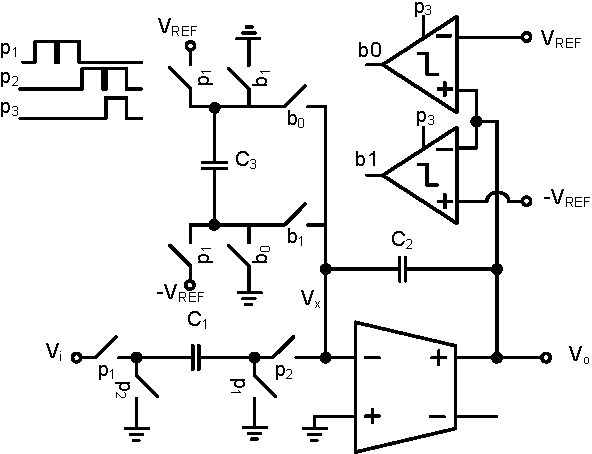
\includegraphics[width=\myfigwidth]{graphics/sc_mod}}
  \caption{Switched-capacitor modulo integrator}
  \label{sdrfig:scmod}
\end{figure}

If $C_1 = C_2 = C_3$ the charge transfer equations implement the
modulo defined in \req{modintdef}. The modulo operation ensures that the
output signal in $p_3$ stays within $V_{o} \in \langle -V_R/2, V_R/2
\rangle$ as long as $V_{i} \in \langle -V_R/2, V_R/2 \rangle$. 

%-------------------------------------------------------
\subsection{Effects of finite gain in modulo integrators}
%-------------------------------------------------------
One of the non-idealities in SC integrators is the
finite opamp gain. The effects of finite opamp gain was covered in \cite{temes80} and
\cite{martin81}.  The transfer function of an integrator with finite
gain can be approximated by 

\eqn{
\label{sdreq:zgainmodap}
\frac{V_o(z)}{V_i(z)} = \dfrac{C_1}{C_2}\dfrac{ a z^{-1}}{1 - b z^{-1}}
}
where
\eqna{
  a &{} = {}& 1-\dfrac{1+C_1/C_2}{A_0}\\
  b &{} = {}& 1-\dfrac{1}{A_0} 
}
and $A_0$ is the DC gain of the opamp. The derivation of this is included in \myappname
\ref{sdrap:intgain}. A block 
model of the modulo integrator is shown in Fig. \ref{sdrfig:modint_beh}.

\begin{figure}[htbp]
\centerline{ 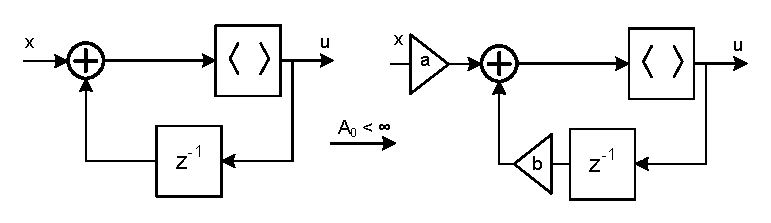
\includegraphics[width=\myfigwidth]{graphics/modint_beh}}
  \caption{ Block model of the modulo integrator for finite DC gain.}
  \label{sdrfig:modint_beh}
\end{figure}

We have assumed that the modulo operation does not influence the
effects of finite gain. To verify the model in
Fig. \ref{sdrfig:modint_beh}  it is implemented in \simulink \cite{simulink} and compared
with two other models, one based on the difference equations
and one based on a SPICE implementation.

An expression can be
derived for the output of a first-order OLSDM using the modulo
arithmetic used in Section \ref{sdrbasicmodulo}. The output of a first
order OLSDM with finite DC gain in the modulo integrators can be
approximated by the difference equation
\eqn{
\label{sdreq:modoutgain}
  y_n = \left \langle x_{n-1} - \dfrac{q_{u,n}}{A_0} + q_n - q_{n-1} \right \rangle_R
}
where $q_{u,n}$ is a white noise approximation of the modulo
integrator output $u_{n}$. The derivation is left for \myappname
\ref{sdrap:finitegain}. 

The
difference between \req{modoutgain} and \req{modout3} is the term $-q_{u,n}/A$. Due to the finite
opamp gain  there is a leakage of $u_n$ to the
output. The modulo integrator output ($u_n$) is a deterministic signal of the input, but we assume it
can be approximated as quantization noise with the limits $q_{u,n} \in
\langle -R/2, R/2 \rangle$. 


From \req{modoutgain} the \textit{signal-to-noise 
and distortion ratio} (SNDR) can be
calculated. For a sinusoidal input the SNDR is
\eqn{
\label{sdreq:osdsndr}
SNDR =  10 \log \left(\frac{A^2/2}{\dfrac{1}{12A_0^2 OSR} +
    \dfrac{LSB^2}{12}\times K}\right)
}
where $A$ is the amplitude of the sinusoid, the first term in the
denominator is the effects of finite gain, and the second term the
quantization noise where $K = 2
\int_0^{f_s/2OSR}{|NTF(z=e^{j\omega})|^2}df$. The calculation of
\req{osdsndr} is left for \myappname \ref{sdrap:sndr}. With $B=7$, $OSR=4$
and $A_0=50dB$ the expected SNDR is 51.3dB. 

%  The two models
% \req{zgainmod} and \req{modoutgain} were compared in a behavioral
% level \matlab simulation. Equation \req{zgainmod} was implemented as
% a z-domain SIMULINK model and Equation \req{modoutgain} was
% implemented as a discrete time difference equation in \matlab. Fig.
% \ref{sdrfig:gainmodel} shows the comparison of the two models and the
% calculated value. Each data point represent the SNDR extracted from a
% $2^{15}$ point FFT for a given input signal frequency. The approximation in \req{modoutgain} differs from
% the calculated value, \req{osdsndr}, because the random values set $q_u$
% in \req{modoutgain}  are chosen randomly from frequency point to frequency
% point. But as we can see from Fig. \ref{sdrfig:gainmodel} the
% approximation has the calculated value as the mean. The z-domain
% model is a more accurate model since it is the signal $u_n$ that leaks
% to the output and not  white noise approximation. As expected the SNDR
% is sligthly higher in the SIMULINK model, since the power of the
% signal $u_n$ is less than the power of $q_{u,n}$. There is also a
% frequency dependence in the SNDR in the SIMULINK model. For low
% frequency input the approximation $u_n \approx q_{u,n}$ is better and
% we see the SNDR aproach eachother. Accordingly, \req{zgainmod} is a
% valid model for the modulo integrator.

%The difference between the SNDR of the two models is
%  less than 1\% for an $OSR=4$, a 7-bit quantizer and a DC gain of
%  40dB. This fortifies the assumption that previous derivations of
%  effects of DC gain can be applied to modulo integrators. 

% \begin{figure}[htbp]
% \centerline{ 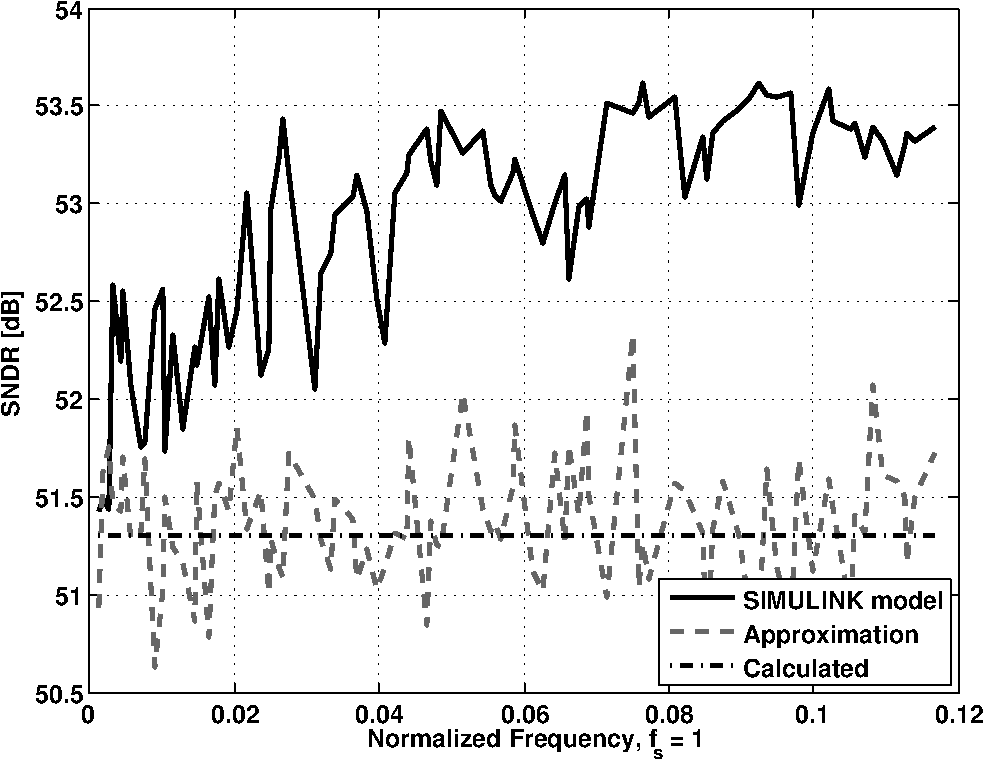
\includegraphics[width=\myfigwidth]{gainmodel}}
%   \caption{ z-domain model of the modulo integrator with DC gain $A < \infty$.}
%   \label{sdrfig:gainmodel}
% \end{figure}

%Fig. \ref{sdrfig:intmod} shows a comparison between the models of the
%low-pass first-order OLSDM (shown in Fig. \ref{sdrfig:olsdm-basic}).
An FFT of the \simulink model (Fig. \ref{sdrfig:modint_beh}) is shown in
Fig. \ref{sdrfig:intmod_z}. Fig. \ref{sdrfig:intmod_d} shows the FFT of the
approximate model as defined by \req{modoutgain}. The FFT of the SPICE model output is shown in
Fig. \ref{sdrfig:intmod_spice}.

 The
approximation in Fig. \ref{sdrfig:intmod_d} is different from the others, here
the noise floor is relatively flat up to $0.01f_s$. At that
point the shaped quantization noise is larger than the leakage from the
integrator output (from \req{modoutgain}) and we get
the high-pass noise shaping. 

For both the \simulink model in Fig.
\ref{sdrfig:intmod_z} and SPICE model in Fig. \ref{sdrfig:intmod_spice} we can
see that the contribution $q_{u,n}/A_0$ is not white, but 
equal to $u_n/A_0$.  Fig. \ref{sdrfig:intmod_u} shows the FFT
of the modulo integrator output ($u_n$) from the \simulink simulations.

The vertical line in the figures denote the
upper bandwidth limit for noise calculation. As a quick estimate of the performance
\req{osdsndr} works well. It overestimates the effects of noise and
has an SNDR of 51.3dB compared to 52.2dB for the \simulink model,
51.66dB in the SPICE model and 51.44dB for the approximation
\req{modoutgain}.  These models show that the modulo operation does
not significantly influence the equations for the effects of finite gain.

Calculation speed is very different in the three models. Calculating \req{osdsndr} takes less than
a second, while the \simulink model take ten seconds for $2^{15}$
points, and the SPICE
simulations take a thousand seconds for $2^{15}$ points. 

To increase the resolution of this first order low-pass OLSDM we can either increase
the quantizer resolution, which we will not do, or reduce the in-band quantization
noise with higher order noise shaping. To get higher order
noise shaping we can increase the
number of zeros in the noise transfer function (NTF) of the
modulator. Either at z=1 (zero frequency) with modulo integrators, or  introduce
zeros at non-zero frequencies. The next section introduces the modulo
resonator, which is used to insert a zero at a non-zero frequency in
the noise transfer function.

\mymodintfig

 
-----------------------------------------------------



%########################################################################
\section{Modulo resonator}\label{sdrmoduloresonator}
%########################################################################

Zeros at non-zero frequency in the noise transfer function reduce the oversampling
ratio for a given quantizer resolution. With zeros at non-zero frequency one can 
implement band-pass sigma-delta modulators. In this section the modulo
resonator is introduced and the ideal and simulated performance
is discussed. 

A model of modulator with zeros at non-zero
frequency can be seen in Fig. \ref{sdrfig:sdrideal}. 
In a world
without signal swing limitations the input signal ($x_n$) can be conditioned
with a resonator, the output of the resonator quantized, and input
signal restored
with a notch filter. The quantization noise will pass through
the notch filter and be filtered accordingly. The output of the
modulator is written as
\eqn{
  Y(z) = STF(z)X(z) + NTF(z)Q(z) 
}
 $STF(z)$ is the signal
transfer function and $NTF(z)$ is the
noise transfer function. 

The input signal pass through
unchanged if the notch filter response matches
the resonator response, thus $STF(z) = 1$.\footnote{The $STF(z)$ will
  probably also contain a time delay, depending on the
  implementation, $STF(z) = z^{-n}$}

 In Fig.
\ref{sdrfig:sdrideal} the $NTF(z)$ is equal to the notch filter response,
which has
a zero at a non-zero frequency.

\begin{figure}[htbp]
\centerline{ 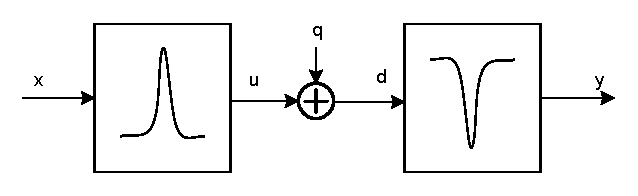
\includegraphics[width=\myfigwidtha]{graphics/sdr_ideal}}
  \caption{Ideal open-loop implementation of NTF zeros at non-zero frequency}
  \label{sdrfig:sdrideal}
\end{figure}

A common resonator used in sigma-delta modulators is based on the lossless discrete
integrator (LDI) \cite{bruton75} shown in Fig. \ref{sdrfig:sdldi}. The
LDI resonator has
a pair of complex conjugate poles at 
\eqn{
  z_p  = \rho \pm j\sqrt(1-\rho^2), \rho = 1-g/2
}
and a resonance frequency of $\omega_0 = cos^{-1}(\rho)$. The
advantage of the LDI is the tunable resonance
frequency. 

\begin{figure}[htbp]
\centerline{ 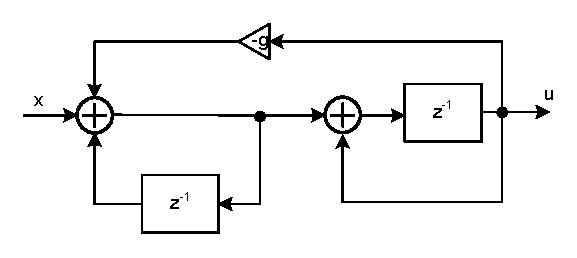
\includegraphics[width=\myfigwidthb]{graphics/sd_ldi}}
  \caption{Resonator based on the lossless discrete integrator (LDI)}
  \label{sdrfig:sdldi}
\end{figure}

If the 
integrators in Fig. \ref{sdrfig:sdldi} are replaced with modulo integrators
we get the modulo resonator shown in
Fig. \ref{sdrfig:sdr_ldi}.  With this modulo resonator 
we can implement Fig. \ref{sdrfig:sdrideal} as shown in
Fig. \ref{sdrfig:sdr_mod}. Fig. \ref{sdrfig:sdr_mod} is a modulo resonator followed by a
linear quantizer and a modulo
notch filter. The modulo operations at the end of the notch filter
reverse the modulo in the resonator. We use two modulo functions in
the notch filter since the modulo is defined as  \req{modintdef}.

%Note that from \req{prop1} we
%should only require one modulo, but the modulus used in Fig. \ref{sdrfig:sdr_mod} are
%defined as \req{limmodulo}.
% The modulo in Fig. \ref{sdrfig:sdr_mod} subtracts or adds
%the range R  once if  $|x_n| \geq R/2$, not infinitely many times as
%\req{modulo}. 

\begin{figure}[htbp]
\centerline{ 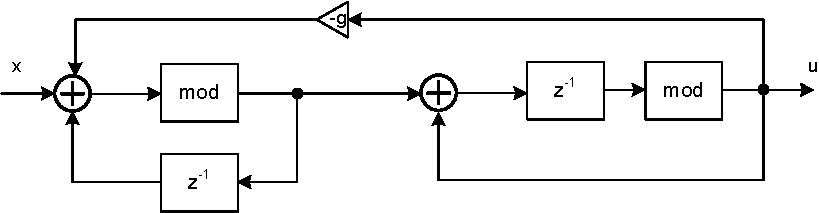
\includegraphics[width=\myfigwidth]{graphics/sdr_ldi}}
  \caption{The modulo resonator }
  \label{sdrfig:sdr_ldi}
\end{figure}

\begin{figure}[htbp]
\centerline{ 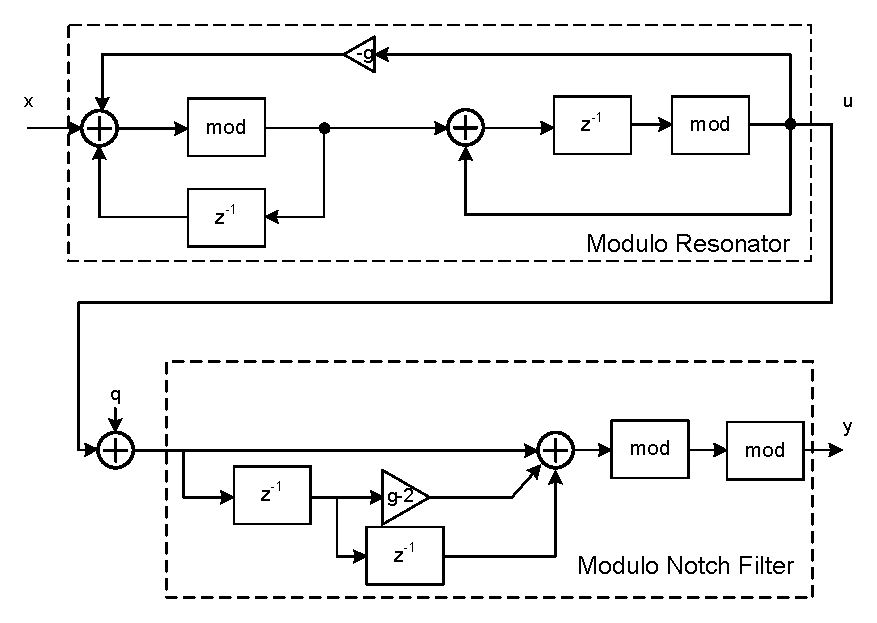
\includegraphics[width=\myfigwidth]{graphics/sdr_mod}}
  \caption{The open-loop sigma-delta modulator with NTF zeros at
    non-zero frequency}
  \label{sdrfig:sdr_mod}
\end{figure}


\begin{figure}[htbp]
\centerline{ 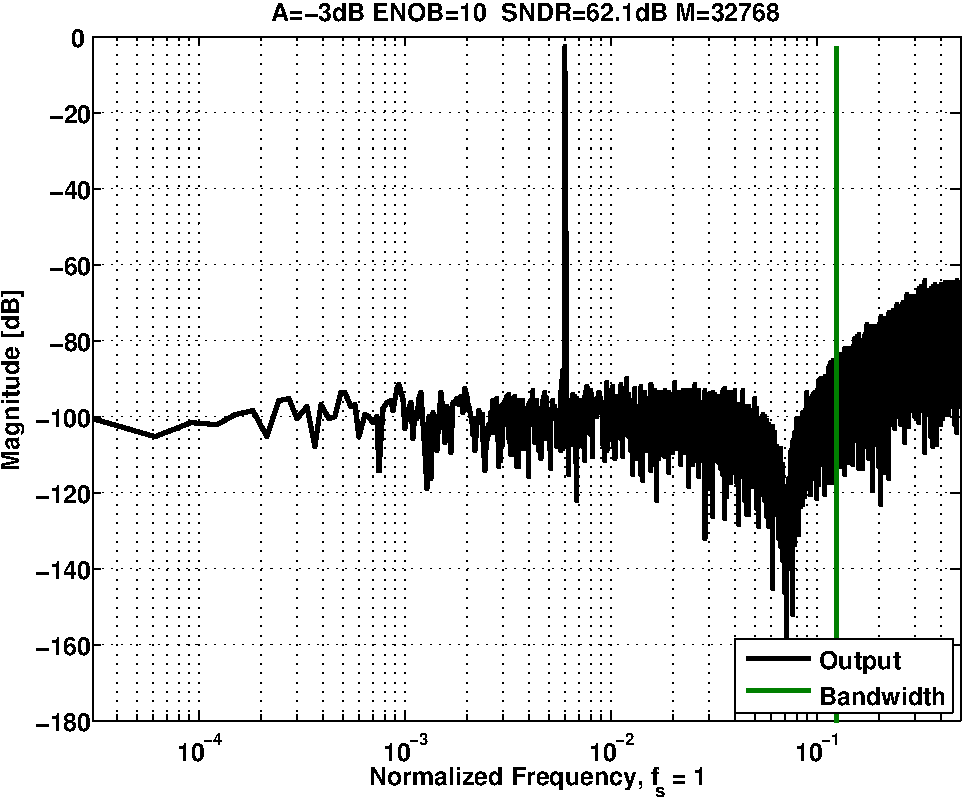
\includegraphics[width=\myfigwidth]{graphics/osdr}}
  \caption{Modulator response. Magnitude of a $2^{15}$ point
    FFT. Input signal amplitude is -3dBFS, input signal frequency is
    at $f_i = 0.006$ with a normalized sampling frequency, $f_s=1$.
  The SNDR with $OSR=4$ is 62.1dB}
  \label{sdrfig:osdr}
\end{figure}


The noise transfer function of the modulator in Fig.
\ref{sdrfig:sdr_mod} is
\eqn{
  NTF(z) = z^2 + (g-2) z + 1
} 
And has an ideal SNDR of 
\eqn{
\label{sdreq:sndr}
SNDR =  10 \log \left(\frac{A^2/2}{2\int_0^{f_s/2OSR}{Q_M^2(f) |NTF(z)|^2}df}\right)
}
if we assume sinusoidal input. Here $Q_M^2(f)$ is the power spectral density of the quantization noise
given by
\eqn{
  Q_M^2(f) = \frac{LSB^2}{12f_s} = \frac{1}{2^{2B}12 f_s}
}
where $LSB = R/2^B$ and $R=1$. 


The optimum zero frequency can be calculated from \req{sndr}. Using an
OSR of four the optimum zero frequency is
$f_i = 0.0718 f_s$ ($g=0.2$). Calculation of the optimum zero
frequencies was covered in detail in \cite{schreier93}.


Fig.
\ref{sdrfig:sdr_mod} was implemented as a \simulink model.
 Fig. \ref{sdrfig:osdr} is a $2^{15}$ point
FFT of the modulator output ($y_n$) with an input signal amplitude of -3dBFS and a
quantization noise power equivalent
to a 7-bit quantizer. Coherent sampling and a Hanning window was used
to avoid spectral leakage of the signal power into neighboring FFT
bins. A brick-wall filter with bandwidth from $0 - f_s/2OSR$ was
used to calculate the SNDR. The
vertical line in Fig. \ref{sdrfig:osdr} denotes the bandwidth. 


For $f_s=1$,
$OSR=4$, $B=7$, $A=1/\sqrt{8}$ the ideal SNDR from \req{sndr} is
62dB. The simulated SNDR match the 
ideal SNDR (1\% difference). 

\subsection{Effects of finite gain in modulo resonators}
Exact analysis of the effects of finite gain in a modulator with a modulo resonator
is complex. The derivation is left for \myappname \ref{sdrap:modresgain}. 

The modulator output
($y_n$ in Fig. \ref{sdrfig:sdr_mod})
 with finite gain in the modulo resonators can be approximated by
\eqn{
  \label{sdreq:modresoest}
  y_n \approx \langle x_{n-1} + (1+g)\epsilon_{p,n-1} + e_n\rangle_R
}
where $\epsilon_p$ is the leakage from the first modulo integrator. The shaped quantization noise is
represented by $e_n$. 
The leakage from the first modulo integrator dominate over the leakage from
the second modulo integrator if the opamp gains in the two
integrators are equal. 


With \req{modresoest} the SNDR is 
\eqn{
\label{sdreq:resapprox}
  SNDR \approx 10 \log\left(\dfrac{ A^2/2}{\dfrac{(1+g)^2}{12
        A_0^2}\dfrac{1}{OSR} + \dfrac{LSB^2}{12}\times K}\right)
}
where $K = \int_0^{f_s/2OSR}|NTF(z)|^2df$. 

Accuracy of
\req{resapprox} depend on the DC gain. It overestimates the SNDR with
1.5dB to 1dB for a DC gain of 60dB - 80dB compared to the
derivation in \myappname \ref{sdrap:modresgain}. But the leakage from the  modulo integrator
is approximated by a white noise source, which  has higher
power than the  power of the actual leakage. Accordingly, the two assumptions: leakage
approximated by a
white noise source, and assuming $\epsilon_p$ is the dominating noise
source, work in opposite directions.

 For
A=-3dBFS, $OSR=4$, $g=0.2$, $LSB=1/2^7$ and a DC gain of
60dB, the approximate SNDR from 
\req{resapprox} is 59.5dB. Whereas for 40dB DC gain the SNDR is
43.1dB. 

Using the previously described modulo integrators in a \simulink
model of
the modulator from Fig. \ref{sdrfig:sdr_mod}, the SNDR is 59.2dB for
60dB DC gain and
42.5dB  for 40dB DC gain. A difference of 0.3dB (4\%) at 60dB DC
gain and 0.6dB (7\%) at 40dB DC gain.

%The next section show how a modulo resonators are combined with
%modulo integrator to produce a more realistic OLSDM, a fifth-order
%low-pass OLSDM with an 
%OSR of four and an ideal SNDR of 85dB.

%########################################################################
\section{Fifth-order low-pass OLSDM}\label{sdrmatlabsim}
%########################################################################
It has previously been shown that the
accuracy of SC circuits depend on the capacitor mismatch, finite DC
gain and unity-gain bandwidth of the opamp
\cite{temes80},\cite{martin81}. We have discussed the effects of
finite DC gain, but left the derivation of capacitor mismatch and
finite unity-gain bandwidth for later
work. But we expect the effects to be similar and limit
the performance to below 14-bit ENOB. This assumes no calibration or
trimming. 

Stages in an OLSDM can be pipelined and it is possible 
to use high latency quantizers such as pipelined ADCs or SAR ADCs. One
in envisioned application of OLSDM is a 14-bit high speed ( 20MS/s) ADC. 
In this section we describe a fifth-order OLSDM with an OSR
of four and 13-bit ENOB.

%-------------------------------------------------------
\subsection{Ideal modulator}
%-------------------------------------------------------
The modulator is  seen in Fig.
\ref{sdrfig:osdr3}. It has two modulo resonators, a
modulo integrator, a 7-bit quantizer, a modulo differentiator, and
two modulo notch filters. To ensure that \req{inlimit} is satisfied 
a gain of 0.9 is inserted between the first and second resonators,
and between the second resonator and the modulo integrator (this is not shown in Fig.
\ref{sdrfig:osdr3}). 

\begin{figure}[htbp]
\centerline{ 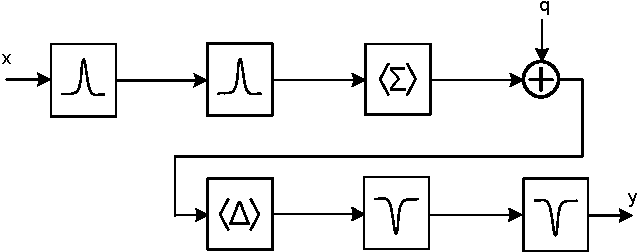
\includegraphics[width=\myfigwidth]{graphics/osdr21_sch}}
  \caption{Fifth-order open-loop sigma-delta modulator}
  \label{sdrfig:osdr3}
\end{figure}

The noise transfer function of the modulator in Fig. \ref{sdrfig:osdr3} is given by
\eqn{
\label{sdreq:fifth_ntf}
  NTF(z) = \frac{(z^2 +(g_1-2)z+1)(z^2 +(g_2-2)z+1)(z-1)}{0.81}
}
And the ideal SNDR can be calculated with \req{sndr}, using the
NTF from \req{fifth_ntf}. With an OSR of four the optimal constants  
are $g_1 = 0.17$ and $g_2 = 0.48$. For $OSR=4$, A=-3dBFS and $B=7$
the ideal SNDR is 85dB. 

A $2^{15}$ point FFT is calculated
from the output of a \matlab simulation of the ideal modulator in Fig. \ref{sdrfig:osdr3}. The FFT
is shown in Fig. \ref{sdrfig:osdr3_ideal}. The simulated match the ideal
SNDR (1\% difference).

The input signal
must be limited as stated in \req{inlimit}.
An input signal amplitude of
-3dBFS $= 1/\sqrt{8} \approx 0.354$ is used in the
simulations.  If we insert for $N=5$
and $B=7$ in the input signal limit \req{inlimit}
\eqn{
  |x(n)| < R(1/2 - 2^{5-1}/2^7) = 0.375
}
Thus the modulator is valid for an input signal amplitude of
-3dBFS.

%The ideal SNDR of the modulator in Fig. 
%\ref{sdrfig:osdr3} is 80.98dB for 
%$A=1/\sqrt{8}$, $OSR=4$, $B=7$ and $f_s=1$. 
%The simulated SNDR =
%80.98dB, which matches the ideal SNDR. 

\begin{figure}[htbp]
\centerline{ \includegraphics[width=\myfigwidth]{graphics/osdr21}}
  \caption{Modulator output. Magnitude of a $2^{15}$ point FFT of the
    modulator output. Input signal amplitude -3dBFS. Input frequency
    $f_i = 0.006$ and sampling frequency $f_s = 1$. With an $OSR=4$
    the SNDR is 84.9dB }
  \label{sdrfig:osdr3_ideal}
\end{figure}

%-------------------------------------------------------
\subsection{Modulator with finite opamp gain in modulo integrators}
%-------------------------------------------------------
Fig. \ref{sdrfig:osdr3g} shows the fifth order sigma-delta modulator with the
the modeled opamp gain. The modulo integrators are
modeled with an
opamp gain
of 85dB in the first resonator, 75dB in second resonator, and 65dB
in the last modulo
integrator. These gains were chosen from design equations based on \req{resapprox}.
Assume the leakage due to 
finite opamp gain in the first modulo resonator dominate. The SNDR is
then estimated from \req{resapprox}. The estimated SNDR for
this modulator is 83.3dB for an input amplitude of -3dBFS.
Fig.
\ref{sdrfig:osdr374} is a $2^{15}$ point FFT of the modulator output ($y_n$)
using an input signal amplitude of -3dBFS. 

\begin{figure}[htbp]
\centerline{ \includegraphics[width=\myfigwidth]{graphics/osdr21g_sch}}
  \caption{Fifth-order open-loop sigma-delta modulator. The DC gain of
    opamps are shown above the stages.}
  \label{sdrfig:osdr3g}
\end{figure}


\begin{figure}[htbp]
\centerline{ \includegraphics[width=\myfigwidth]{graphics/osdr21g}}
  \caption{Magnitude of a $2^{15}$ point FFT of the modulator
    output. Input signal amplitude -3dBFS, input frequency $f_i =
    0.006$ and sampling frequency $f_s = 1$. With an $OSR=4$ the SNDR=80.9dB}
  \label{sdrfig:osdr374}
\end{figure}

The simulated SNDR is
 80.9dB (13.15-bit ENOB\footnote{ENOB = (SNDR-1.76)/6.02}), or 2.4dB below the estimated SNDR. This is expected due to
leakage from later stages. If we increase the DC gain in the second
modulo resonator and the last modulo
integrator to 200dB, we remove
them as noise contributors. This increases the SNDR to 82.8dB, which
is 0.5dB (6\%) lower than the estimated. 

The
modulator in Fig. \ref{sdrfig:osdr3g} was implemented in SPICE as a switched
capacitor circuit. 



%-------------------------------------------------------
\subsection{Switched capacitor modulator}
%-------------------------------------------------------
Fig.
\ref{sdrfig:osdr3spice} shows a switched-capacitor implementation of
the modulator. A single ended modulator was used for simplicity. 
\begin{figure}[htbp]
\centerline{ \includegraphics[width=\myfigwidth]{graphics/osdr21_spice_sch}}
  \caption{Fifth order OLSDM SPICE model. Quantization and NTF are implemented in \matlab}
  \label{sdrfig:osdr3spice}
\end{figure}

The opamps have a DC gain of 85dB, 85dB, 75dB, 75dB, and 65dB.
The opamp was implemented as a macro-model of a single-pole operational amplifier.

A
comparison between the \matlab model and the SPICE model is shown in
Fig. \ref{sdrfig:fifthordersdm}, here a $2^{15}$ point FFT was run on both
the SPICE and the \matlab outputs. The SNDR is the same for both
models. In SPICE, however, there is more harmonic content, with the second
harmonic visible in the FFT.

The quantizer and NTF for the SPICE simulations is implemented in
\matlab. A 7-bit ideal quantizer is used instead of the linear
approximation to quantization noise. 

\begin{figure}[htbp]
\centerline{ \includegraphics[width=\myfigwidth]{graphics/osdr21_spice}}
  \caption{Comparison of SPICE model and \matlab model. Input signal amplitude -3dBFS, input frequency $f_i =
    0.006$ and sampling frequency $f_s = 1$. With an $OSR=4$ the
    SNDR is 80.9dB for the \matlab model and 80.9dB for the
    SPICE model.}
  \label{sdrfig:fifthordersdm}
\end{figure}

\subsubsection{Capacitor mismatch}
In modern CMOS processes the matching between capacitors is good. In a
typical 90nm process the matching of two 10pF Metal-Insulator-Metal
(MIM) capacitors can be as good as 0.06\% (3 sigma). In the
switched-capacitor OLSDM matching will influence the coefficients, and
the inter-stage gain. The matching in the first stage is most critical,
as mismatch in later stages is attenuated by the gain of the previous
stage. With a mismatch in the coefficients and inter-stage gain the
digital transfer function (from the quantizer and out) will not have
the correct coefficients. This will lead to noise
leakage, since the poles of the analog filter (the two resonators and
the integrator) will not match the zeros in the digital filter (the
two notch filters and the differentiator). 

With 0.06\% matching between capacitors the SNDR degrades to 79.7dB, which is not
significant. But the capacitor sizes in a switched-capacitor
implementation will be determined by the most critical capacitor, the
$g_1C$ capacitor in the first stage. In this example $g_1 = 0.17$,
which is small. With mismatch taken into consideration it might be
advantageous to move resonator with the $g_2 = 0.48$ first, even
though this will increases the noise leakage somewhat. The unit capacitor
$C$ can be chosen smaller since the $g_2C$ capacitor must match to
0.06\% (3 sigma). With $g_1C$ as the first capacitor the unit capacitor must be
almost three times larger than if the $g_2C$ capacitor is used as the
first capacitor.

\subsubsection{Comparator Offset}
 A concern with a switched-capacitor implementation is the offset in
 the comparators used in the modulo resonator. Simulations suggest
 that the stochastic offset of comparators in the modulo resonator
 must be within 0.25\% of full-scale to have an SNDR of
 above 77dB. Achieving an offset on this level requires rigorous analog
 design. At offset of 1\% of full-scale the SNDR degrades
 to 65dB. For example, with a full-scale of 2V peak-to-peak we tolerate
 an offset of $\pm 5mV$ in the comparator thresholds.


%74dB osdr3_l -6dB 11.05 vs 11.04 in model with N=2048



%########################################################################
\section{Conclusion}
%########################################################################
In this paper we introduced the modulo resonator for open-loop
sigma-delta modulators (OLSDM). It was used with a modulo notch filter to
introduce a zero in the noise transfer function at a non-zero
frequency. The modulo resonator and previously published modulo
integrator were used in a behavioral model of a switched-capacitor fifth-order OLSDM with more
than 13-bit effective number of bits for an oversampling ratio of
four. We proved that the number of bits in the quantizer (B) must be
larger than the order of the modulator (N) to ensure equivalence between OLSDM and sigma-delta
modulation.


%\appendices
\myappendices

\section{Proof  of  modulo theorem}
\label{sdrap:modproof}
\begin{IEEEproof}
From definition 
\eqn{
\label{sdreq:roundmodulo}
\langle a + nR\rangle_R = \langle a \rangle_R
}
where $n$ is an integer. Given
\eqn{
  \langle \langle x \rangle_R + \langle y \rangle_R \rangle_R
}
we can write $\langle x \rangle_R = x-nR$ and $\langle y \rangle_R = y
- mR$, where $n$ and $m$ are integers. From \req{roundmodulo} it follows that
\eqn{
  \langle x - nR + y - mR \rangle_R = \langle x + y \rangle_R
}
\end{IEEEproof}

\section{Effects of finite gain in SC integrators}
\label{sdrap:intgain}
If we assume infinite DC gain in the opamp the
charge transfer equation is simply
\eqn{
\label{sdreq:intchargez}
  C_2 V_{o,n} = C_2 V_{o,n-1}  + C_1 V_{i,n-1}
}
The z-domain transfer function of  \req{intchargez} is
\eqn{
\label{sdreq:intzdomain}
\frac{V_o(z)}{V_i(z)} = \frac{C_1}{C_2}\frac{z^{-1}}{1-z^{-1}}
}
If $C_1 =C_2$, then \req{intzdomain} is the well known transfer function of
a discrete time integrator and is a good approximation if the
DC gain ($A_0$) is much higher than the accuracy required. If the DC gain is close to,
or lower than the accuracy, then \req{intzdomain} no longer applies.

With finite opamp gain the voltage $V_x$ (in Fig. \ref{sdrfig:scint}) will be different from
zero. A non-zero $V_x$
will result in  a
residual charge on capacitor $C_1$ given by $Q_{1,n} = C_1
V_x$. The
charge transfer equation change into
\eqn{
\label{sdreq:chgain}
  Q_{2,n} = Q_{2,n-1} + Q_{1,n-1} + Q_{1,n}
}
where $Q_2 = C_2 (V_o - V_x)$, $Q_{1,n-1} = C_1 V_i$. The residual
voltage $V_x$ is equal to $V_x = -V_o/A_0$. We define
\eqn{
\alpha = 1 + \frac{1}{A_0}
}
If we expand \req{chgain} we get
\eqn{
\alpha V_{o,n}  = \alpha V_{o,n-1}  + \frac{C_1}{C_2}
V_{i,n-1} - \frac{C_1}{C_2} \frac{V_{o,n}}{A_0}
}
Solved for $V_o/V_i$ and transferred to the z-domain we get the
transfer function
\eqn{
\label{sdreq:zgainexact}
\frac{V_o(z)}{V_i(z)}  = \dfrac{C_1}{C_2} \dfrac{\left(\dfrac{1}{1 + \dfrac{1+
      C_1/C_2}{A_0}}\right)z^{-1}}{1 - \alpha \left(\dfrac{1}{1 + \dfrac{1+
      C_1/C_2}{A_0}}\right) z^{-1}}
}
If we assume $A_0>>1$, then \req{zgainexact} can be approximated to first
order by
\eqn{
\label{sdreq:zgainmodap1}
\frac{V_o(z)}{V_i(z)} = \dfrac{C_1}{C_2}\dfrac{\left(1 -
  \dfrac{1+C_1/C_2}{A_0}\right)z^{-1}}{1 - \left(1 - \dfrac{1}{A_0}\right) z^{-1}}
}

\section{Effects of finite gain in modulo integrators}
\label{sdrap:finitegain}
From charge transfer equations the output of the modulo integrator is
\eqn{
  \alpha u_n = \left \langle \alpha u_{n-1} + x_{n-1} - u_n/A_0 \right \rangle_R
}
where $\alpha  = 1+1/A_0$ and $A_0$ is the DC gain of the opamp. We
also have
\eqn{
  \alpha u_{n-1} = \left \langle \alpha u_{n-2} + x_{n-2} - u_{n-1}/A_0 \right \rangle_R
}
and that
\eqn{
  \alpha u_{n-2} = \left \langle \alpha u_{n-3} + x_{n-3} - u_{n-2}/A_0 \right \rangle_R
}
Using \req{prop1} the output of the modulo integrator is 
\setlength{\arraycolsep}{0.0em}
\begin{eqnarray}
\label{sdreq:apintout}
u_n &{}={}& \dfrac{\left \langle \sum_{i=0}^\infty{x_{n-1-i}\alpha^i} -
  \sum_{i=0}^\infty{\dfrac{u_{n-i}}{A_0}\alpha^i} \right \rangle_R}{\alpha}\nonumber\\
&{}={}& \left \langle \sum_{i=0}^\infty{x_{n-1-i}\alpha^{i-1}} -
  \sum_{i=0}^\infty{\dfrac{u_{n-i}}{A_0}\alpha^{i-1}} \right \rangle_R\nonumber\\
\end{eqnarray}
\setlength{\arraycolsep}{5pt}

The output of the modulator is 
\eqn{
y_n = u_n - u_{n-1} + q_n - q_{n-1}
}
using \req{prop1} and \req{apintout}
\eqn{
 y_n = \left \langle \dfrac{x_{n-1}}{\alpha} - \dfrac{u_n}{A_0\alpha} +
 q_n - q_{n-1} \right \rangle_R
}
Assuming $A_0 >> 1$ we can approximate the modulator output by
\eqn{
\label{sdreq:modapprox1}
  y_n = \left \langle x_{n-1} - \dfrac{u_n}{A_0} + q_n - q_{n-1} \right \rangle_R
}
The signal $u_n$  can be
written as \req{modint_copy}. This signal is the quantization noise
after rounding the integrator output to the range R. We assume this
quantization noise is white. Assume $u_n \approx q_{u,n} \in \langle -R/2,
R/2 \rangle$. Then \req{modapprox1} simplifies to 
\eqn{
\label{sdreq:modapprox2}
  y_n = \left \langle x_{n-1} - \dfrac{q_{u,n}}{A_0} + q_n - q_{n-1} \right \rangle_R
}

\section{Calculation of the SNDR}
\label{sdrap:sndr}

The power spectral density of quantization noise is given by the
well known equation
\eqn{
  Q^2(f) = \dfrac{LSB^2}{12 f_s}
}
where $f_s$ is the sampling frequency. For a given bandwidth the noise
power is
\eqn{
  Q^2 = 2\int_0^{f_s/2OSR} Q^2(f)df = \dfrac{ LSB^2}{12}\dfrac{1}{OSR}
}
The LSB of $q_{u,n}/A_0$ can be written as $R/A_0$. And if we assume $R=1$
the noise power of the modulo integrator output leakage is given by
\eqn{
\label{sdreq:osdnu}
  Q_u^2 = \dfrac{1}{12 \times A_0^2}\dfrac{1}{ OSR}
}   
The quantization noise in a first order OLSDM is high-pass filtered, and has a
noise transfer function of
\eqn{
  NTF(z) = 1-z^{-1}
}
The LSB of the quantization noise is $LSB = R/2^B$, so with $R=1$ the
quantization noise power can be calculated from 
\eqn{
\label{sdreq:osdnp}
  Q_{n}^2 = 2\int_0^{f_s/2OSR}{\dfrac{1}{12 \times 2^{2B} f_s} |NTF(z=e^{j\omega})|^2}df
}
The signal to noise and distortion ratio can be written as 
\eqn{
  SNDR = 10 \log\left( \dfrac{A^2/2}{Q_u^2 + Q_n^2}\right)
}
and inserted for \req{osdnu} and \req{osdnp} gives
\eqn{
\label{sdreq:osdsndr1}
SNDR =  10 \log \left(\frac{A^2/2}{\dfrac{1}{12A_0^2 OSR} +
    \dfrac{LSB^2}{12}\times K}\right)
}
where
\eqn{
K =
2\int_0^{f_s/2OSR}{|NTF(z=e^{j\omega})|^2}df
}

\section{Effects of finite gain in modulo resonators}
\label{sdrap:modresgain}
We start with the difference
equations for the output of the integrators in the modulo
resonator. And we assume that the modulo has no
effect. The output of the first modulo integrator is given by
\eqn{
  \alpha p_n = (1+g)\alpha p_{n-1} + x- g u_n  - (1+g)\epsilon_p 
}
where $\epsilon_p = p_u/A_0 \approx q_p/A_0$ is the leakage as described earlier for
modulo integration and $\alpha = 1 + 1/A_0$, where $A_0$ is the DC
gain. The leakage is now $(1+g)$ larger than for a single modulo integrator, which is due to the
feedback capacitor given by $gC$ in Fig. \ref{sdrfig:osdr3spice}. The
feedback capacitor increase the residual charge since the voltage
$V_x$ in the modulo integrator is now forced across a larger
capacitance $C + gC$. The output of the modulo resonator is written as
\eqn{
  \alpha u_n = \alpha u_{n-1} + p_{n-1} - \epsilon_u
}
where $\epsilon_u = u_n/A_0 \approx q_u/A_0$ is the leakage from the
second modulo integrator.
Transferring to the z-domain and solving the equations for $u$ we get
\eqn{
\label{sdreq:mrgainu}
 U(z) = \dfrac{x z^{-1}}{B(z)} - \dfrac{(1-z^{-1})\alpha\epsilon_u}{B(z)} -
 \dfrac{(1+g)\epsilon_p z^{-1}}{B(z)}
}
where $B(z)$ is
\eqn{
  B(z) =\alpha^2 z^{-2} + (g-2\alpha^2)z^{-1} + \alpha^2
}
After the modulo resonator the signal is quantized and filtered by the
notch filter. The notch filter transfer function is equal to the noise
transfer function. The NTF can be written as\footnote{Here we have
  shifted the NTF in time by multiplying by $z^{-2}$}
\eqn{
NTF(z) = z^{-2} + (g-2)z^{-1} + 1
}
and we see that if $\alpha = 1$ then $NTF(z) = B(z)$. 


The output of the modulator will be 
\eqn{
\label{sdreq:aprgmodout}
Y(z) = U(z) \times NTF(z) + Q(z) \times NTF(z)
}
inserted for \req{mrgainu} in \req{aprgmodout}
\eqna{
\label{sdreq:mrgainout}
  Y(z) &{}={}& \dfrac{NTF(z)}{B(z)}\left[x z^{-1} + (1-z^{-1})\alpha \epsilon_u +
    (1+g)\epsilon_p z^{-1}\right] \nonumber\\
&{}+{}& Q(z) \times NTF(z)
}
There are three effects that can be seen from \req{mrgainout}. The
leakage from the first integrator $\epsilon_p$ leaks directly to the
output scaled by a factor $1+g$. The leakage from the second integrator, $\epsilon_u$, is first order high
pass filtered. The finite gain in the modulo
integrators cause an incomplete pole/zero cancellation between
the NTF(z) and B(z), for low DC gain this will increase the noise
contribution. For high DC gain we can assume that $\alpha \approx 1$
such that $NTF/B(z) \approx 1$. Then \req{mrgainout} becomes
\eqna{
    Y(z) &{}={}& X(z) z^{-1} + (1-z^{-1}) \epsilon_u +
    (1+g)\epsilon_p z^{-1} \nonumber\\
&{}+{}& Q(z) \times NTF(z)
}
Transferred back to time domain we have the difference
equation
\eqn{
\label{sdreq:aprgmodoutdf}
  y_n = \langle x_{n-1} + \epsilon_{u,n} - \epsilon_{u,n-1} +
  (1+g)\epsilon_{p,n-1} + e_n\rangle_R
}
where $e_n$ is the shaped quantization
noise.

 The dominating noise source in \req{aprgmodoutdf} is the
the leakage from the first integrator ($(1+g)\epsilon_{p,n-1}$). The
modulator output can thus be approximated by

\eqn{
  y_n \approx \langle x_{n-1} + (1+g)\epsilon_{p,n-1} + e_n \rangle_R
}





%%% Local Variables: 
%%% mode: latex
%%% TeX-master: "ieee_resonator"
%%% End: 



\renewcommand{\figurename}{Figure}
\renewcommand{\myfignamehead}{Figure}

\chapter{Paper 4}\label{sc:p4}
\textbf{\Large 0.8V 1GHz Dynamic Comparator In Digital 90nm CMOS
  Technology}\\
%\newline
\indent   Carsten Wulff and Trond Ytterdal\\
\indent In proceedings of the 23rd NORCHIP Conference, 2005. \\
\indent 21-22 Nov. 2005 Pages 237 - 240 \\
\indent Digital Object Identifier: 10.1109/NORCHP.2005.1597033\\

\renewcommand\myfigname{p1fig:}
\renewcommand\myeqname{p1eq:}

\section*{Errata}
\begin{itemize}
\item Section 7.2, second paragraph, third sentence: What way
  $\rightarrow$ Which way
\item Section 7.3, fifth paragraph, second sentence: to threshold
  $\rightarrow$ to the threshold
\end{itemize}

%\textbf{Abstract:}
\begin{abstract}
The design of a 0.8V 1GHz dynamic comparator in digital 90nm
CMOS technology is presented. The work will show that low voltage, low
power and high speed analog circuits are feasible in nano-scale CMOS
technologies. The dynamic comparator dissipates a maximum of
222\begin{math}\mathrm{\mu}\end{math}W at 1GHz clock frequency with
100fF capacitive load and 0.8V supply voltage. This is lower than
comparable results. 
\end{abstract}


\section{Introduction}

One of the factors driving the downscaling of CMOS technology is the
ever present drive for price-per-performance of digital circuits. The
minimum dimensions get smaller and maximum supply voltages are reduced
due to reliability issues \cite{iwai99}.
%[1]
Since digital circuits are the driving force of silicon technology,
analog circuit designers often have to work in digital CMOS processes.
The reduction in supply voltage is not necessarily followed by an equal
reduction in threshold voltage, which limits the available voltage
headroom \cite{annema05}. 
%[2]
These nano-scale CMOS technologies offer many challenges that have
been discussed in previous publications, among others \cite{iwai99,annema05,annema04}.
%[1-3]
The challenges have, in some cases, brought success to simpler
topologies \cite{draxelmayr04}
%[4]
that have shown some of the advantages of nano-scale CMOS for analog
circuits. One advantage of scaling down is the increased speed that
follows. It can be shown that the unity gain frequency
(\textit{f$_{UG}$}) of a transistor is proportional to the effective
gate voltage (\textit{V$_{GT}$}) over the square of the length
(\begin{math}L\end{math}) of a transistor as given by (\ref{p1eq1})
%(1)
\cite{annema05}
%[2]
\eqn{
\label{p1eq1}
  f_{UG} \propto \dfrac{V_{GT}}{L^2}
}

Thus the trend will be that shorter lengths bring higher speeds.

Dynamic comparators are a class of circuits often used in pipeline
analog to digital converters (ADCs) \cite{cho95}.
%[5]
 As the name suggests a pipeline ADC consists of multiple stages. It
is common to extract at least 1.5-bits in each stage. The 1.5-bits per
stage stem from a digital error correction algorithm that requires a
certain redundancy in the number of bits. With the digital error
correction comparators in each stage can have quite large offset. Using
1.5-bits per stage one can tolerate a comparator offset of up to
\begin{math}\pm{}\end{math}V$_{REF}$/4, where V$_{REF}$ is the high
reference voltage minus the common mode voltage. In general, the
comparators can tolerate an offset up to
\begin{math}\pm{}\end{math}V$_{REF}$/2$^{b}$ for a b-bit stage
\cite{sumanen00}.
%[6]
Using dynamic comparators may reduce the architectural complexity
and reduce power dissipation, but tight control over variations and
mismatch must be exercised to ensure that offset and other errors are
kept within the allowed limits. Architectures that reduce mismatch have
been presented \cite{sumanen00}.
%[6]
In this paper, we describe a dynamic comparator that is a
modification of MOSFET-only fully-differential dynamic comparator
presented in \cite{lofti03}.
%[7]
 We will first describe the architecture and operation of the
comparator before we present the design in 90nm CMOS and simulation
results.
 

\section{Dynamic comparator architecture}

The circuit can be seen in Figure \ref{p1fig:dccomp}. In \cite{lofti03}
%[7]
they used a clock booster to supply a higher voltage to M1-M4 than
the supply voltage. To avoid any reliability concerns that may come
with boosted voltages we have replaced the clock booster with a single
transistor M5. The comparator has two phases; Reset and Latch. In the
Reset phase the latch, shown by the back to back inverters, is shorted
to ground through M6 and M7. To stop current flowing through the
shorted inverters M5 is turned off. Notice that both operations are
accomplished by a transition on CLK from low to high. This resets the
output of the comparator to zero and place INV1 and INV2 in a known
state. For the comparator to work properly it is important that INV1
and INV2 are reset to a known state, any unintentional imbalance
between the two inverters might tip the comparator towards one side.
 
When the clock goes from high to low we enter the Latch phase. In this
phase the inverters are connected in a positive feedback loop. What way
the latch will swing is controlled by an intentional imbalance in the
supply to the inverters. This imbalance is controlled by the
transistors M1-M4. Depending on their gate voltages transistors M1-M4
have variable on-resistance. For the moment we will ignore transistors
M2 and M3. If M1 and M4 are matched, their on-resistances will be the
equal when the differential input voltage (V$_{INPUT}$) is zero (VIN =
VIP). When V$_{INPUT}$ is negative (VIN \begin{math}>\end{math} VIP) M4
will turn more off, and the resistance in M1 will be lower than
resistance in M4. Thus INV1 will be slightly faster than INV2, and the
comparator will settle to VOP equals zero and VON equals one. The
opposite will occur if the V$_{INPUT}$ is positive (VIP
\begin{math}>\end{math} VIN). Notice that this comparator does not need
multiple clocks or inverted clocks, one clock signal is sufficient to
trigger transition from one phase to another and back again.
 

\begin{figure}[htbp]
\centerline{\includegraphics[width=\myfigwidth]{img0}}
  \caption{Dynamic comparator}
  \label{p1fig:dccomp}
\end{figure}

As stated, with M2 and M3 ignored the comparator has a threshold at
V$_{INPUT}$ = 0. However, in a 1.5-bit pipeline stage we need two
comparators with the thresholds given by eqs. (\ref{p1eq2})
and (\ref{p1eq3}) \cite{sumanen00}.  The transistors M2 and M3 serve to offset the threshold of the
comparator. They add small amounts of current to the two branches and
intentionally tip the balance of the comparator. Ideally we would scale
M2 and M3 to one fourth of the width of M1 and M4. However, as we will
se later, this is different in a real process.
 
\eqn{
\label{p1eq2}
V_{INPUT} = + \frac{1}{4}V_{REF}
}
\eqn{
\label{p1eq3}
V_{INPUT} = - \frac{1}{4}V_{REF}
}


We have two reference voltages, high and low. These are common mode
plus V$_{REF}$ and common mode minus V$_{REF}$, respectively. With the
high and low reference voltages connected to VRP and VRN, respectively,
the threshold will be set at (\ref{p1eq2})
%(2)
. If we reverse the connections to VRP and VRN we set the threshold at
(\ref{p1eq3})
%(3)
.
 


The boundary conditions for the inverters play an important role in
deciding which way the comparator swings. If we have large difference
in e.g. the capacitive load at the output of the inverters the
comparator might swing the wrong way. Therefore, we keep the load
controlled by using two matched buffers at the output of the inverters.
We have chosen a high reference at 0.6V and a low reference at 0.2V.
The common mode is set at 0.4V. Thus, the maximum allowable offset in
this work is \begin{math}\pm{}\end{math}V$_{REF}$/4 =
\begin{math}\pm{}\end{math}0.2V/4 = \begin{math}\pm{}\end{math} 50mV.
Simulations will show that the comparator stays within this limit.
 

Mismatch between transistors can influence the offset of the
comparator. Mismatch of MOSFET transistors can be reduced by increasing
the area of the transistor \cite{pelgrom89}. We tried to keep transistor areas as large as possible in order to
reduce mismatch, while small enough to keep capacitances low. All
transistors have a length of 0.1\begin{math}\mathrm{\mu}\end{math}m to
maximize the speed, according to (\ref{p1eq1}). All PMOS devices have a width of
3\begin{math}\mathrm{\mu}\end{math}m and all NMOS devices have a width
of 1.2\begin{math}\mathrm{\mu}\end{math}m as seen in Table \ref{p1tab:p1_widths}. Devices are kept
at the same width to simplify layout to maximizing the matching
\cite{johns}. Notice that the effective width, width x Number of Unit Devices in
parallel (NUD), of M1 and M2 does not correspond to a scaling of
one-fourth.  In the 90nm process we are using a scaling of eight was
necessary to keep the threshold at the reasonable level. M6 and M7 are
the twice the effective width of the NMOS transistors in the inverters.

\begin{table}[htbp]
\centering
\renewcommand{\arraystretch}{1.3}
\caption{ Transistor widths and fingers. $^{1}$NUD:  Number of Unit Devices in parallel }
\label{p1tab:p1_widths}
\begin{tabular}{l|l|l}
\hline
\textbf{Transistor}&\textbf{Width (\begin{math}\mathrm{\mu}\end{math}m)}&\textbf{NUD$^{1}$} \\
\hline
M1 \& M4 & 3.0
&
16
 \\
\hline
M2 \& M3
&
3.0
&
2
 \\
\hline

M5
&
3.0
&
84
 \\
\hline
M6 \& M7
&
1.2
&
2
 \\
\hline
\end{tabular} 
\end{table}

 

\section{Simulation Results}

Some of the key parameters for this dynamic comparator are offset,
delay and power dissipation. The offset needs to be within plus/minus
one-fourth of the reference voltage, which in our case corresponds to
\begin{math}\pm{}\end{math}50mV. We aimed for a speed of 1GHz at 0.8V.
This corresponds to a maximum delay of 500ps from CLK goes low to
output is valid. Remember that the comparator has two phases; Reset and
Latch, they need 500ps each at 1GHz clock frequency with a 50\% duty
cycle. We have not considered other duty cycle arrangements.

Since we were primarily considering high speed and low voltage, we did
not set any requirements for power dissipation. However, dynamic
comparator power dissipation resembles that of digital gates, which
have a power dissipation given approximately by:

\eqn{
\label{p1eq4}
  P = f C V_{DD}^2 + V_{DD}I_0
}

Where \begin{math}f\end{math} is the output frequency,
\textit{V$_{DD}$} is the supply voltage, \begin{math}C\end{math} is the
output capacitance and \textit{I$_{0}$} is the average leakage current
\cite{vittoz94}
%[10]
. With a low supply voltage and limited capacitance we anticipated
reasonable power consumption.


Simulations were performed in five process corners; Fast, Typical,
Slow and cross corners (fast NMOS, slow PMOS and visa versa). We also
ran three temperature corners (-40$^{o}$, 0$^{o}$, 85$^{o}$) for each
process corner. In addition, Monte Carlo simulations were performed to
simulate the effect of mismatch. All transistors included a model of
gate leakage current. A capacitive load of 100fF was used at the output
of the buffers in all simulations. Each parameter (offset, delay and
power dissipation) was extracted in each of the corners. Typical values
were extracted from typical process corner. The standard deviation
(\begin{math}\sigma{}\end{math}) for power dissipation and offset was
extracted from a Monte Carlo simulation. For offset it was around 3 mV
for both high and low threshold. For power dissipation the standard
deviation was negligible. We subtracted 3\begin{math}\sigma{}\end{math}
from the minimum value and added 3\begin{math}\sigma{}\end{math} to the
maximum value of offset and power dissipation. Table \ref{p1tab:p1_offset} shows the
results for comparator offset and power dissipation including
3\begin{math}\sigma{}\end{math}.  The offset is within
\begin{math}\pm{}\end{math}25mV which is well below the required
\begin{math}\pm{}\end{math}50mV. The maximum power dissipation was
222\begin{math}\mathrm{\mu}\end{math}W, almost half of this was
dissipated in the output buffers. As previously stated we have used a
similar architecture to that of \cite{lofti03}. They achieved 100\begin{math}\mathrm{\mu}\end{math}W with 200fF at
50Msamples/s and 1V in a 0.25\begin{math}\mathrm{\mu}\end{math}m CMOS
technology. Since most of the power dissipation in this architecture is
dynamic we can use (\ref{p1eq4})
to compare the two results.  If we scale the results from \cite{lofti03}
to 1GHz with 100fF and 0.8V we get a power dissipation of
640\begin{math}\mathrm{\mu}\end{math}W. Thus, a maximum power
dissipation of 222\begin{math}\mathrm{\mu}\end{math}W at 1GHz with
100fF and 0.8V can be considered reasonable.
 


Simulating delay in a comparator requires that one choose the input
signal with care. It can be shown that the delay of latched comparators
becomes large when the differential input voltage is close to threshold
\cite{johns}. We simulated the delay around the threshold by applying a
differential ramp at the input from 20mV above the ideal threshold to
20mV below the ideal threshold using 200 clock periods running at 1GHz.
The change in input from one clock period to the next was around
200\begin{math}\mathrm{\mu}\end{math}V. It is difficult to know exactly
where the threshold of the comparator is. We therefore used the delay
of the second pulse after the comparator switched states. By doing this
we know we never measure delay exactly at the threshold, but always
within 200\begin{math}\mathrm{\mu}\end{math} -
400\begin{math}\mathrm{\mu}\end{math}V away from the threshold. As with
offset and power dissipation, a Monte Carlo simulation was performed to
get the \begin{math}\sigma{}\end{math} of the delay. The
\begin{math}\sigma{}\end{math} of the delay decreased as we moved away
from the threshold. The standard deviation of the delay for the first
pulse after threshold was up to 30-50ps for high and low thresholds,
most of which we believe is due to varying distance to threshold when
the comparator latches. The \begin{math}\sigma{}\end{math} of the delay
for the second pulse was below 10ps, it is this
\begin{math}\sigma{}\end{math} that has been used in Table  \ref{p1tab:p1_offset}. In the
worst corner and including 3\begin{math}\sigma{}\end{math} variation in
delay due to mismatch, the comparator has less than 400ps delay. This
would give us a maximum clock frequency of 1.25GHz, but allowing for a
safety margin we choose 1GHz as maximum.
 


If the differential input voltage is closer than
\begin{math}\pm{}\end{math}200\begin{math}\mathrm{\mu}\end{math}V to
the threshold, less than what was used in simulation, there is a chance
of metastability. Metastability is when the comparator has larger delay
than the available settling time. A detector for metastability can be
inserted after the comparator \cite{kinniment99}. A XOR port connected to VON and VOP, with delay much smaller than
the comparator, will give a one if there is no metastability and zero
if there is metastability. This is ensured by the reset to zero of both
outputs in the Reset phase. In a case of metastability one can
arbitrarily choose output state of the comparator since one knows that
the input is close to threshold, much closer than the required
\begin{math}\pm{}\end{math}50mV. However, when using a metastability
detector one must make sure that the pull-down delay of Reset plus
delay of the detector is less than half the clock period. In this
design the pull-down delay in Reset was below 200ps. We have not yet
considered effects of layout parasitics.
 

\begin{table}[htbp]
\centering
\renewcommand{\arraystretch}{1.3}
\caption{ Offset, power dissipation and delay}
\label{p1tab:p1_offset}
\begin{tabular}{l|l|l|l|l}
\textbf{Parameter}
&
\textbf{Min}
&
\textbf{Typ}
&
\textbf{Max}
&
\textbf{Unit}\\
\hline

Offset (High threshold)
&
-22.5
&
9
&
15
&
mV
 \\
\hline
Offset (Low threshold)
&
-16
&
8.5
&
22
&
mV
 \\
\hline
Power diss.@1GHz
&
180
&
193
&
222
&
\begin{math}\mathrm{\mu}\end{math}W
 \\
\hline
Delay
&
80
&
186
&
\begin{math}<\end{math} 400
&
ps
 \\
\hline
\end{tabular}
 
\end{table}

\section{Future work}

The comparator is scheduled for production in a digital 90nm CMOS
technology during fall of 2005. The main purpose of the prototype is to
verify the rather small variations due to process variation and
mismatch seen in simulations. If the prototype confirms what has been
seen in simulations the comparator will be used in scheduled high
performance ADCs.
 

\section{Acknowledgements}
Financial support from the Norwegian Research Council through the
project Smart Microsystems for Diagnostic Imaging in Medicine (project
number 159559/130) and the project ASICs for Microsystems (project
number 133952/420) is gratefully acknowledged.
 

\section{Conclusion}
The design of a 0.8V 1GHz dynamic comparator in digital 90nm CMOS
technology has been presented. The work shows that low voltage, low
power and high speed analog circuits are feasible\textit{ }in
nano-scale CMOS technology. The dynamic comparator dissipates a maximum
of 222\begin{math}\mathrm{\mu}\end{math}W at 1GHz clock frequency with
100fF capacitive load at a supply voltage of 0.8V which is lower than
comparable results. Table  \ref{p1tab:p1_summary} shows a summary of simulation results.
 
 



 



 



 



 
\begin{table}[htbp]
\centering
\renewcommand{\arraystretch}{1.3}
\caption{ Summary of simulation results}
\label{p1tab:p1_summary}
\begin{tabular}{l|l}
Offset
\begin{math}<\end{math} \begin{math}\pm{}\end{math} 25mV
 \\
\hline
Clock Frequency
&
\begin{math}>\end{math} 1GHz
 \\
\hline
Power dissipation
&
\begin{math}<\end{math} 222\begin{math}\mathrm{\mu}\end{math}W
 \\
\hline
Supply voltage
&
0.8 V
 \\
\hline
Clock signals
&
1
 \\
\hline
High reference
&
0.6V
 \\
\hline
Low reference
&
0.2V
 \\
\hline
Common mode
&
0.4V
 \\
\hline
\end{tabular}
\end{table}



 

%\section{References}



 

% \begin{enumerate}
% 	\item \styleReferences{Iwai, H.; \textquotedblleft{}CMOS technology-year
% 2010 and beyond \textquotedblleft{}. Solid-State Circuits, IEEE Journal
% of Volume 34,~ Issue 3,~ March 1999 Page(s):357 - 366}
% 	\item \styleReferences{Annema, A.J.; Nauta, B. ; van Langevelde, R.;
% Tuinhout, H.; \textquotedblright{}Analog Circuits in
% Ultra-Deep-Submicron CMOS\textquotedblright{}. IEEE Journal of Solid
% State Circuits, Vol 40. 1. January 2005. Pages: 133-143}
% 	\item \styleReferences{Annema, A.J.; Nauta, B.; van Langevelde, R.;
% Tuinhout, H.; \textquotedblleft{}Designing outside rails
% constraints\textquotedblright{}. IEEE Int. Solid-State Circuits Conf.
% (ISSCC) Dig. Tech. Papers, 2004, Pages: 134-135}
% 	\item \styleReferences{Draxelmayr, D; \textquotedblleft{}A 6b 600MHz 10mW
% ADC Array in Digital 90nm CMOS\textquotedblright{}. IEEE Int.
% Solid-State Circuits Conf. (ISSCC) Dig. Tech. Papers, 2004}
% 	\item \styleReferences{Cho,T.H.; Gray, P.R; \textquotedblright{}A 10 b, 20
% Msample/s, 35mW Pipeline A/D Converter\textquotedblright{}, IEEE
% Journal of Solid-State Circuits. Vol. 30. NO. 3. March 1995,
% Pages:166-169}
% 	\item \styleReferences{Sumanen, L.; Waltari, M.; Halonen, K.;
% \textquotedblleft{}A mismatch insensitive CMOS dynamic comparator for
% pipeline A/D converters \textquotedblleft{} Electronics, Circuits and
% Systems, 2000. ICECS 2000. The 7$^{th}$ IEEE International Conference
% on Volume 1,~ 17-20 Dec. 2000 Pages:32 - 35 vol.1}
% 	\item \styleReferences{Lofti, R; Taherzadeh-Sani, M; Yaser Azizi, M; Shoaei,
% O; \textquotedblleft{} A 1-V MOSFET-only fully-differential dynamic
% comparator for use in low-voltage pipelined A/D
% converters\textquotedblright{}, Signals, Circuits and Systems, 2003.
% SCS 2003. International Symposium on
% \\
% Volume 2,~ 10-11 July 2003 Page(s):377 - 380 vol.2}
% 	\item \styleReferences{Pelgrom, M.J.M.; Duinmaijer, A.C.J.; Welbers, A.P.G.;
% \textquotedblleft{}Matching properties of MOS
% transistors\textquotedblright{} Solid-State Circuits, IEEE Journal of
% Volume 24,~ Issue 5,~ Oct 1989 Page(s):1433 \textendash{} 1439}
% 	\item \styleReferences{Johns, D.; Martin, J.; \textquotedblleft{}Analog
% Integrated Circuit Design\textquotedblright{}. John Wiley \& Sons,
% Inc., 1997}
% 	\item \styleReferences{Vittoz,E.; \textquotedblleft{}Micropower
% techniques\textquotedblright{}. Design of VLSI circuits for
% Telecommunication and Signal Processing. Chapter 5, Prentice Hall,
% 1994}
% 	\item \styleReferences{Kinniment, D.J.; Yakovlev, A.V.;
% \textquotedblleft{}Low power, low noise micropipelined flash A-D
% converter\textquotedblright{}. Circuits, Devices and Systems, IEE
% Proceedings. Volume 146,~ Issue 5,~ Oct. 1999 Page(s):263 - 267}
% \end{enumerate}



 



  


%%% Local Variables: 
%%% mode: latex
%%% TeX-master: "tb_paper1"
%%% End: 

\chapter{Paper 5}\label{sc:p5}
\textbf{\Large Design of a 7-bit 200MS/s, 2mW Pipelined ADC With Switched
  Open-Loop Amplifiers In a 65nm CMOS Technology}\\
\indent Carsten Wulff and Trond Ytterdal\\
\indent In proceedings of the 25th NORCHIP Conference, 2007.\\
\indent  Digital Object Identifier 10.1109/NORCHP.2007.4481042 \\
\renewcommand\myfigname{p2fig:}
\renewcommand\myeqname{p2eq:}
%\section{Abstract}

\begin{abstract}
We present the design of a
7-bit 200MS/s pipelined ADC with switched open-loop amplifiers in a
65nm CMOS technology. As a
result of turning
off the open-loop amplifiers during sampling we reduce the power
dissipation by 23\%. The ADC achieves a SNDR
of 40dB close to the Nyquist frequency, with a power dissipation of
2mW, which results in a 
Walden FOM of 0.13pJ/step and a Thermal FOM of 1.6fJ/step.
\end{abstract}


%-------------------------------------------------------
\section{Introduction}
%-------------------------------------------------------
Low resolution high speed ADCs have historically been
Flash based architectures. The Flash ADC is a fast architecture due to
it's parallel nature. However, it is a very inefficient
architecture. One of the
reasons for its inefficiency is that it is not possible, with current
processing technology, to get the input capacitance down to what is
the minimum required by thermal noise. This is mostly due to parasitic
capacitances from transistors and metal routing. 

Before we begin our argumentation we should define what we mean with
parasitic capacitances. We define parasitic capacitance as; any
capacitance that is not required by the operation of the circuit.

% For
%example in a standard sample and hold the only required capacitance in our
%circuit would be the sampling capacitance, as shown by Figure
%\ref{p2fig:samplehold}. 
%Parasitic capacitances at the sampling node
%include the transistor capacitances (Cgd Cdb), sampling
%capacitor parasitics (Cp), input capacitance of next stage (Cin) and routing
%capacitances (Cmet).

%\myfigure{samplehold}{ Sample and hold with buffer, parasitics are
%  represented by gray capacitances.}{samplehold}

One of the fundamental error sources that limit the performance of ADCs is the thermal noise power,
which is usually represented as
%\eqn{
%\label{p2eq:thermpower}
%$\overline{V_{thermal}^2(t)} = \frac{a\times k T}{C}$
%}
$\overline{V_{thermal}^2} = a\times k T/C$
where a is a constant, k is Boltzmann's constant, T is the temperature
in Kelvin and C is the sampling capacitance. 

%Thermal noise also manifests
%through sampling jitter, but in a 7 bit ADC at 200Msps jitter is not the
%dominating error source. \footnote{Jitter in an ADC is a sum of the
%  source jitter from the clock and the clock phase generating circuit
%  in the ADC. In the clock phase generating circuit the jitter with a white power spectral density is usually caused by
%  thermal noise}

Thermal noise power sets the lower limit for how much power we must
dissipate to achieve a certain SNR. With respect to thermal noise
power a certain SNR usually translates into a certain sampling
capacitance. 

%If we assume the least significant bit (LSB) is given by
%\eqn{
%V_{LSB} = \frac{V_{max}}{2^{bits}}
%}
%which leads to a quantization noise power of
If we assume a quantization noise power of
%\eqn{
%$\overline{V_{LSB}^2(t)} = \frac{V_{LSB}^2}{12}= \frac{V_{max}^2}{2^{2bits}\times
%  12}$
$\overline{V_{LSB}^2} = V_{LSB}^2/12= V_{max}^2/(2^{2bits}\times
  12)$
%}
, and we assume $\frac{1}{4}\overline{V_{LSB}^2} = \overline{V_{thermal}^2}$ and
$a = 1$, the equation for the required sampling capacitor is
\eqn{
\label{p2eq:capval}
C = \frac{48 k T 2^{2bits}}{V_{max}^2}
}

If we use 6 bits, $k=1.38\times10^{-23} J/K$, $T=353 K$ and $V_{max} = 0.4V$ 
the required sampling capacitance is 6fF. This, of course, assumes that other concerns like
mismatch or unwanted effects from parasitic capacitances does not come
in to play.

%In an ideal world this would be the largest capacitor in our ADC, and
%the power dissipation would be proportional to this capacitor. However, in current nanoscale technology it is not uncommon to get in
%excess of 10fF parasitic capacitance at circuit nodes. 
%So a 6fF sampling capacitance is smaller than the parasitic
%capacitance. Because of this, we will use more power to charge and
%discharge parasitic capacitances than the needed sampling capacitance,
%through this we waste power. 

%And often it will not be possible to have
%a sampling capacitor of 6fF because the parasitics will affect the
%circuit operation, which is the case with the pipelined ADC we present
%in this paper. In pipelined ADC with open-loop amplifiers, the input
%capacitance of the amplifier  decreases the gain of the
%multiplying DAC, as explained in \cite{Shen07}.

Parasitics at a node can reach 10fF in current nanoscale
technologies, as a consequence the parasitics can be larger than required
sampling capacitor at the 6-bit level. This is
one reason why a Flash ADC looses when it comes to
efficiency. A 6-bit Flash ADC without averaging or interpolation has 64 comparators connected
to the input, each of which has possibly 10fF input capacitance. Thus
a Flash ADC can have 600fF input capacitance, which is two orders of magnitude larger than the
required sampling capacitance. 

If we look at the figure of merit (FOM) of 6-bit ADCs, and higher
resolution ADCs, using the Walden FOM \cite{walden99} given by
\eqn{
FOM = \frac{P_{diss}}{2^{bits}f_s}
}
where $P_{diss}$ is the
power dissipation and $f_s$ is the sampling frequency. And the Thermal
FOM given by 
\eqn{
\label{p2eq:thermfom}
FOM = \frac{P_{diss}}{2^{2bits}f_s}
}
We get  Figure \ref{p2fig:waldenthermal}, with the gray
diamonds representing Walden FOM and the black triangles representing
Thermal FOM. The data for Figure
\ref{p2fig:waldenthermal} was collected from ADCs published in the Journal of
Solid State Circuits in the years 1975-2005. According to the Walden FOM there
are 6-bit ADCs that are just as good as the 15-bit ADCs, since they
have the same figure of merit. However, the Walden FOM is an
empirically deduced FOM, and it has come
under some scrutiny in the recent years. A more theoretically
correct FOM is the Thermal FOM.\footnote{As far as we
  know the FOM has not yet been given a name, so the name Thermal FOM
  is not an official name. It is, however, a descriptive name.}

\myfigure{graphics/waldenthermal}{ Walden FOM versus Thermal FOM as a function
  of bits for ADCs published in the
  Journal of Solid State Circuits 1975-2005. Thermal FOM in black and
  Walden FOM in gray.}{waldenthermal}
%\myfigure{thermal}{ Thermal FOM as a function of bits for ADCs in
%  Journal of Solid State Circuits 1975-2005}{thermal}

The argument for why the Thermal FOM is more correct is as follows. Assume a thermal noise limited ADC, where
the power dissipation is proportional to the sampling
capacitance. 
If we increase the resolution by one bit, we can see from
(\ref{p2eq:capval}) that the sampling capacitance quadruples, and
through this the power dissipation quadruples.
However, the Walden FOM only allows a doubling of the
power dissipation for each bit of resolution added. This leads to an
unfair FOM for high number of bits and a lenient FOM for low
number of bits. 

%If we re-plot the data from Figure \ref{p2fig:waldenthermal}
%with the FOM given by \ref{p2eq:thermfom} we get Figure
%\ref{p2fig:thermalthermal}. 


%Most of this difference is because low
%resolution ADCs are not close to being limited by thermal noise.

Two alternatives to Flash ADCs have received some attention in recent years. The first is
successive-approximation (SAR) ADCs and the second is pipelined ADCs. Both
have in recent papers achieved good results. 

%In \cite{draxelmayr04}
%they achieved a Thermal FOM of 20fJ/step with a time interleaved SAR
%ADC. 
In \cite{Chen06} they presented a
6-bit 600MS/s time interleaved asynchronous successive-approximation
ADC, with a Walden FOM of 0.22pJ/step and a Thermal FOM of
5.7fJ/step. In \cite{Shen07} they presented a 6-bit pipelined ADC with open-loop
amplifiers achieving a Thermal FOM of 59fJ/step.
Note that the best 6-bit ADC in Figure \ref{p2fig:waldenthermal}, is 
\cite{lin02} with a Thermal FOM of 16.38fJ/step, which is three orders of magnitude worse than
the best $>$ 14-bit ADCs. And the best 7-bit ADC is a 100kS/s SAR
\cite{Scott03} with a Thermal FOM of 1.89fJ/step, which is two orders of magnitude worse than the best
$>$ 14 bit ADCs.
% None of these get
%close to the apparent Thermal FOM limit of $0.01fJ/step$ in Figure \ref{p2fig:waldenthermal}, achieved by some of the
%higher resolution converters. 
%It is probably not possible to get close
%to this limit in current
%technologies, but it is interesting to see how close one can get at
%reasonably high speed. 

Our goal for this design was to optimize the FOM for a low resolution
ADC at a resonable speed. 
We choose to design a pipelined ADC and placed it
at the conservative speed of 200MHz. That is, the speed is
conservative if we compare to the speed to
\cite{Shen07} or \cite{Chen06}. Usually, low resolution ADCs are used
in the GHz range, so we assume that the this pipelined ADC would be
used in a time interleaved architecture. Knowing that we would be unable
to use a 6fF sampling capacitor we opted for 7-bit resolution, since
the thermal noise power would anyway be low because of the larger
sampling capacitor, and adding one more stage
does not increase the power significantly. To keep parasitic
capacitances from transistors as low as possible we chose to use a
65nm CMOS technology. The pipelined ADC architecture is
explained in the following section with results of simulations
presented in Section \ref{p2results}.


%------------------------------------------------------------------------
\section{Pipelined Architecture}\label{p2arch}
%------------------------------------------------------------------------
The ADC was designed in a 65nm low power CMOS technology with low threshold
voltage (lvt) transistors. 
The architecture of the differential pipelined ADC is shown in Figure \ref{p2fig:pipe}. The ADC has
five 1.5-bit pipelined stages and a three level flash at the end. Each stage has a three level analog to
digital converter (SADC) and a multiplying DAC (MDAC). The MDAC has a gain of
two. 

\myfigure{graphics/pipe}{Architecture overview of the 7-bit Pipelined ADC with open-loop amplifiers}{pipe}

%It has been tradition to use switched capacitor circuits with
%high gain opamps to achieve the accurate gain of two. However, high
%gain opamps are difficult to design in nanoscale technologies, like
%the 65nm CMOS we choose for this design. The problem is the low output
%conductance of the transistors, and it is not uncommon with an
%intrinsic gain (gm/gds) of 10. For an accuracy of 7-bit in a closed
%loop switched capacitor circuit we would need
%a gain of around 46dB, which would require at least two stages (or
%gain boosting) in 65nm technology. 

One of the alternatives to the traditional operational amplifiers in MDACs is an open-loop amplifier,
like a common source amplifier, with a gain of two. This technique has
been used with success in a 12-bit pipelined ADC \cite{murmann03}
and 6-bit pipelined ADC \cite{Shen07}. Our design is based on
\cite{Shen07}. The MDAC architecture can be seen in
Figure \ref{p2fig:stage12}. Figure \ref{p2fig:stage12} shows stage one and stage
two. Stage one is in the amplifying phase, the SADC has made its
decision, and the control signals t0, t1 and t2 control transmission
gates that connect one of the two sampling capacitors to high
reference, common mode or low reference. The control signals t0, t1, t2
and the transmission gates implement the DAC. Stage two is shown
in the sampling phase. Here both capacitors are connected to the
input through transmission gates controlled by clock ip1. Each stage
needs three clock phases, p1, p1a and p2, where p1a is slightly advanced
over p1, and is used to sample the input when it is quiet. p1 and p2
are non-overlapping clock phases. Stage two uses ip1, ip1a and ip2, where
ip1=p2 and ip2=p1. All in all we need four clock phases for the
complete pipelined ADC, p1, p1a, p2 and p2a. The open-loop amplifier
is marked by x2 in Figure 
\ref{p2fig:stage12}. 
%The transmission gates
%and the SADC have been designed such that the number of clock signals
%is kept at a minimum, thus there are only four clocks signals distributed from
%the clock buffers. 


\myfigure{graphics/stage12}{ Stage 1 and stage 2 in the pipelined ADC}{stage12}

%------------------------------------------------------------------------
\subsection{Open-Loop Amplifier}
%------------------------------------------------------------------------

A detailed schematic of the open-loop amplifier can be seen in  Figure
\ref{p2fig:openamp}. It is a differential common source amplifier with
resistive load. The resistors are each $4k\Omega$, and we assume that they
will be calibrated at startup, so the resistor value is constant over
process. In this differential amplifier it is important that the common
mode variation is low. If not, the common mode voltage will drift as
the signal propagates through the pipelined stages, and may even turn later
stages off. To achieve low common mode variation we use a replica bias that
keeps the total current, $I_{tot} = I_{R1} +I_{R2}$, equal to two times
$I_{bias}$ over process, voltage and temperature variations. Through
this the common mode voltage is determined by 
%\eqn{
$V_{cm} = V_{dd} -  I_{tot}/2 \times (R1+R2)/2 $
%}
which keeps it constant over process and temperature variation. 

The
transistors M5/M6/M1/M2 are twice the size of M7/M8/M11/M12, as a
consequence $I_{tot} = 2I_{bias}$. We choose the common mode to be
0.6V, to get larger overdrive on the input transistors, and the swing
to be $\pm 0.2V$.

The gain of the common source amplifier, if we disregard the source
degeneration, is given by $A_o = g_{m1}R_1$
%
%\eqn{
%
%}
%where $g_{m1}$ is given by
%\eqn{
%g_{m1} = \frac{2I_d}{V_{gs} - V_{th}}
%}
%$g_{m1} = 2I_d/(V_{gs} - V_{th})$. 
%With $I_{tot}$ constant the transconductance varies over process due to
%changes in the threshold voltage, $V_{th}$. The variation in $V_{th}$ will change the gain
%of the amplifier. 
The gain will vary over process and temperature because of changes in
$g_m$, we compensate for some of this change by varying the vctrl
voltage of the source degeneration transistor, which  in effect
changes the effective source degeneration resistor and in turn changes
the gain of the amplifier. If we include the
source degeneration the gain
expression becomes
\eqn{
A_o = \frac{g_{m1}R_1}{1 + \frac{g_{m1}}{2 g_{ds13}}}
}

\myfigure{graphics/openamp}{ Open-Loop Amplifier}{openamp}

In \cite{Shen07} they used a replica MDAC stage configured in a feedback
loop to control the vctrl voltage such that the MDAC stage has a gain
of two. Since we only do simulation we have not included the replica
stage, the  vctrl voltage is  changed manually for each corner simulation. 

The gain of the MDAC is also affected by the input capacitance of the
amplifier as described in \cite{Shen07}.

Our main contribution to reduce the power of the pipelined ADC is the
transistors M3/M4, these turn off the the amplifier during sampling
phase when it is not needed. Because the drain and source nodes of
M3/M4 are low impedance, and the bias voltage, vb, stays constant,
the amplifier turns on quickly. 

In our design the bias current is  $I_{bias} = 100 \mu A$, which makes
the total current consumption of a MDAC stage $300 \mu A$, ergo the
power dissipation of five MDAC stages should be $1.5 mW$, assuming we
use a 1V supply. This is if we leave
the amplifiers on all the time. By turning off the amplifiers during sampling
the power dissipation is reduced to $P_{mdacs} = 5 \times 100 \mu A \times 1V+ \frac{1}{2}{5
  \times 200 \mu A} \times 1V = 1mW$, so we would expect an improvment
of 0.5mW when the amplifiers are turned off during sampling.

With this low current in the amplifiers, the input capacitance of the
next stage must be low. The sampling capacitors (C1, C2) are chosen at
50fF. The reason for choosing such a large value
compared to the required, is not capacitor matching concerns, which do not
come in to play at 7-bit, but rather the parasitic capacitance from
the amplifier input, which reduces the gain of the MDAC. We
compensate for some of this reduction in gain with the vctrl voltage.

Two other circuits dissipate power in the pipelined ADC, the SADCs and
the clock generator/buffers. The size of the clock buffers are mainly determined by
the load of the SADCs and routing capacitance. The power dissipation
in the SADCs are
determined by matching concerns of the comparators. The comparators used are the so
called Lewis-Gray
dynamic comparators introduced in \cite{cho95}. 

%------------------------------------------------------------------------
\subsection{Clock Generation}
%------------------------------------------------------------------------
Most
switched capacitor circuits use two non-overlapping clocks to control
the charge transfer, but since
we use bottom plate sampling there is an advanced phase 1 that transitions just
before phase 1. The advanced clock phase reduce the problem of input dependent charge injection
from the input switches. 

We use NMOS inputs in the comparators
due to the high common mode voltage, thus the comparators use a clock that
samples on the rising edge. To avoid distributing inverted clock
phases we invert the clocks of the transmission gates, which means that the
transmission gates are on when the clock signal is low, and off when
the clock signal is high. The clock buffers were scaled to drive 6 SADCs,
transmission gates, amplifier turn-off control signal and a 100fF
capacitance was added at the output of each clock buffer to model the the parasitic
capacitance added by metal routing.

%------------------------------------------------------------------------
\section{Results of Simulation}\label{p2results}
%------------------------------------------------------------------------
The ADC was simulated at transistor
level using Eldo from Mentor Graphics. A common mode of 0.6V, and a
swing of 0.2V, as previously mentioned, resulted in a differential
peak to peak of 0.8V with a 1V supply. Both the references and inputs are assumed to be
buffered off-chip, the buffers are not included in the simulation. Results of
Eldo simulations were post-processed in MATLAB, were an FFT was
performed and signal-to-noise-and-distortion (SNDR) was extracted.
In all simulations an input signal frequency close to the Nyquist frequency
was used, and an input signal amplitude of 0.8 times full scale range.

Mismatch simulations were performed in the typical corner at a
temperature of 27 degrees Celcius. A $2^7$ point FFT was used to estimate the
SNDR and 101 simulations were run to get an estimate of the standard
deviation of the SDNR due to mismatch. The mean SNDR was 40dB and the standard
deviation was 1.2dB. 

Four process corners (fast, slow, fast-slow, slow-fast) and three
temperature corners ($0^o, 27^o, 80^o$) were simulated. 
%Power supply
%voltage variation was also simulated, and it was found that the ADC
%breaks down at around 0.95V in slow corner down to speed issues. A positive shift
%in supply, to 1.1V, could be compensated with changing vctrl. 
When we vary vctrl to compensate for the threshold voltage changes, the
standard deviation in SDNR over process corners and temperature
corners is 2.35dB, with the worst corner being slow process and low
temperature. With constant vctrl the standard deviation increases to 3.45dB.

Figure \ref{p2fig:noise} shows an $2^{10}$ point FFT of the output from
a transient simulation with noise in the typical corner.  

\myfigure{graphics/siphon_fft}{A 1024 point FFT of the ADC output from a transient
  noise simulation. The harmonics of the fundamental are marked with diamonds.}{noise}

The total power dissipation for the simulated ADC in typical corner
(typical process, $27^o$ and 1V supply) is 2mW. If we leave the
amplifiers turned on during sampling it dissipates 2.6mW, with the increase being close
to the expected 0.5mW. Table
\ref{p2tab:performance} summarizes the achieved performance in the
typical corner.

The
Walden FOM of the ADC is 0.13pJ/step and the  Thermal FOM of
1.6fJ/step. 
The improvement is almost a factor four compared to the Thermal FOM of
5.7fJ/step from \cite{Chen06}, bearing in mind that they have proven
silicon, and that the difference might be eaten up by layout
parasitics. In addition, we operate at a lower speed and a higher SNDR,
which makes it more straightforward to achieve a good figure of merit. However, \cite{Chen06} was a SAR while our ADC is
a pipelined ADC, making the point the two architectures can compete on
equal grounds with respect to figure of merit at reasonable speeds.

%The Thermal FOM of our ADC is still two orders of magnitude worse than
%the apparent ``thermal limit'' of 0.01fJ/step. 
%Much of this can be
%explained by small, but still the relatively large sampling
%capacitors of 50fF, if we compare to the required sampling capacitor
%of around 6fF. Even in a state of the art technology, like the 65nm
%CMOS, it is difficult to design a pipelined ADC
%which is limited by thermal noise.  

 
\begin{table}[ht]
\centering 
\caption{Preformance summary of the 7-bit Pipelined ADC}
\begin{tabular}{l|r}
\label{p2tab:performance}
Technology & 65nm LP CMOS\\
Input Voltage Peak-to-Peak & 0.8V\\
Supply Voltage & 1V \\
Sampling Frequency & 200MHz\\
SNDR & 40dB \\
ENOB & 6.3dB \\
Power Dissipation & 2mW \\
Walden FOM & 0.13pJ/step\\
Thermal FOM & 1.6fJ/step\\
\end{tabular}

\end{table}

\section{Future Work}
Low resolution pipelined ADCs with open-loop amplifiers make for an
interesting architecture, it may well be the most efficient, straightforward way
to implement high speed low resolution ADCs at the present time. 
More work is needed to try to reduce the sampling capacitance,
and we believe that cutting the parasitic capacitances down, through
architecture or technology changes, is the most effective way
to increase effectiveness of high speed low resolution ADCs.


\section{Conclusion}
We presented the design of a
7-bit 200MS/s pipelined ADC with switched open-loop amplifiers in a
65nm CMOS technology. As a
result of turning
off the open-loop amplifiers during sampling the power dissipation was
reduced by 23\%. The ADC achieved a SNDR
of 40dB close to the Nyquist frequency, with a power dissipation of
2mW, which resulted in a 
Waldon FOM of 0.13pJ/step and a Thermal FOM of 1.6fJ/step.


%------------------------------------------------------------------------
\section*{Acknowledgments}
%------------------------------------------------------------------------
Financial support from the Norwegian Research Council through the
project Smart Microsystems for Diagnostic Imaging in Medicine (project
number 159559/130) and the project ASICs for Microsystems (project
number 133952/420) is gratefully acknowledged.

%-------------------------------------------------------
%Figures
%-------------------------------------------------------


%\bibliography{IEEEabrv,/home/wulff/svnwork/wulff/work/ntnu/phd/phd,/home/wulff/svnwork/wulff/work/ntnu/phd/IEEE_J_JSSC.bib}


%\end{document}

\renewcommand{\figurename}{Fig.}
\renewcommand{\myfignamehead}{Fig.}
\chapter{Paper 6}\label{sc:p6}
\textbf{\Large Design and Behavioral Simulation of Comparator-Based Switched
  Capacitor Circuits}\\
\indent Carsten Wulff and Trond Ytterdal\\
\indent Accepted at 26th NORCHIP Conference 2008\\
\renewcommand\myfigname{cdesfig:}
\renewcommand\myeqname{cdeseq:}

\section*{Errata}
\begin{itemize}
\item Section 9.7, third paragraph, fifth line: 11\% should be 16\%
\end{itemize}


\begin{abstract}
Design equations are a required tool in the  analog designers
toolbox. In this paper we show how one can calculate the required
parameters for 
comparator-based switched-capacitor circuits for use in a pipelined ADC. The parameters are
capacitance ($C$), current ($I_0$), comparator delay ($T_d$), current
source output resistance ($R_o$) and comparator threshold 
($V_{ct}$). The design equations
are verified with behavioral simulations in SPICE and MATLAB.
\end{abstract}


%\keywords{
%\paragraph{Keywords}
\begin{keywords}
 Comparator-based switched-capacitor circuits, design equations,
 pipelined analog-to-digital converters
\end{keywords}
%}
\section{Introduction}
\IEEEPARstart{D}{ownscaling} of CMOS technology continue to challenge the analog
designer. Reduced power supply, due to reliability concerns
\cite{iwai99}, and reduced
transistor output resistance, due to shorter channels
\cite{annema05}, lead to low headroom and low intrinsic
gain. As a consequence, high DC gain
operational amplifiers (opamp) | the key component in most
switched-capacitor circuits | is hard to design in nano-scale
technologies. 

Techniques like correlated level shifting
\cite{gregoire08}, open-loop residue amplifiers \cite{murmann03}, gain calibration \cite{hernes07},  and
comparator-based switched-capacitor circuits (CBSC)  \cite{sepke06} have been
developed to solve  some of the challenges. The techniques either reduce the
gain requirements for a given resolution, or replace the
opamp completely. 


Introduced in
\cite{sepke06} CBSC is a completely new approach to switched-capacitor
circuits. It replaces the opamp with a comparator and a current
source. To demonstrate the technique a prototype 10-bit 8-MS/s 
2.5-mW pipelined ADC was presented at ISSCC 2006  \cite{sepke06}. The implementation was detailed in
\cite{fiorenza06}.
%A
%year later a 200-MS/s 8-bit 8.5-mW Zero-Crossing-Based pipelined ADC,
%which replaced the comparator with a zero-crossing detector,
%was presented \cite{brooks07}. These implementations were
%explained in more detail in
%\cite{fiorenza06} and \cite{brooks07a}. 

In this paper we discuss how to design CBSC circuits for
analog-to-digital converters. 

Before one starts simulating transistors in SPICE it is of utmost
importance to have a clear idea of the dominating error sources, and
how they should be handled. In that respect, tools like design
equations, mathematical simulations and behavioral SPICE simulations
are invaluable tools for the analog designer.

\paragraph{Design Equations}
 Based on the specification (how fast, how accurate, how
    little power) the parameters for different circuit blocks can be
    calculated. The design equations result in a place to start, a set of
    initial parameters to work with. 
\paragraph{Mathematics based simulation}
 Behavioral
  simulation in a mathematics based tool, like MATLAB or
  OCTAVE, is more complex than design equations, but more
  accurate. But it is still fast and a designer can sweep parameters
  to find optimal solutions.
\paragraph{SPICE simulation}
Behavioral level description in SPICE allow the designer to have a
top-level description of the circuit, with all circuit blocks defined.   
The functionality of circuit blocks is checked before circuit blocks
 are implemented with transistors. 

This paper is organized as follows: Section \ref{cdessc:opamp} review opamp based
switched-capacitor circuits. Section \ref{cdessc:cbsc} explain
comparator-based switched-capacitor circuits. A model of the output
voltage of a CBSC amplifier with a gain of two is described in Section
\ref{cdessc:outmod}. In Section \ref{cdessc:design}
we introduce a design methodology for CBSC circuits and show a design
example in Section \ref{cdessc:example}. Results of
simulations in MATLAB and SPICE verify our design equations in Section \ref{cdessc:sims}.


%-------------------------------------------------------
\section{Opamp based switched-capacitor circuits} \label{cdessc:opamp}
%-------------------------------------------------------
%switched-capacitor circuits are prevalent in  ADCs
%because of their robustness and accuracy. Doing
%arithmetic operations like summation, subtraction, multiplication 
%and division is possible in SC circuit with high accuracy. The
%accuracy of SC circuits is limited by capacitor matching, which can be
%accurately set in integrated circuits (on the order of 0.1 percent \cite{johnsmartin}).  

Switched-capacitor (SC) circuits are usually designed with an opamp feedback loop as shown in
Fig. \ref{cdesfig:sccmult}. Most SC circuits have two clock phases,
sampling and charge transfer. Fig. \ref{cdesfig:sccmult} is a  
amplifier where the input is sampled in phase $p_1$, and charge is
transferred from
$C_1$ to $C_2$ in $p_2$ by forcing $V_x$ to
ground. If the opamp has infinite gain the discrete time transfer
function for Fig. \ref{cdesfig:sccmult} is a  delayed
amplification, where the gain is determined by the capacitance
ratio.
\eqn{
H_0(z) = \frac{C_1+C_2}{C_2} z^{-1}
}
With finite gain in the opamp the transfer function is
\eqn{
H_1(z) = H_0(z) \times\frac{1}{1+(C_1/C_2+1)/A}
}
where $A$ is the DC gain of the opamp.  Finite gain in the
opamp reduce the gain of the SC amplifier.  For the remainder of this work we assume $C_1 = C_2$, so the
amplifier has a gain of two.

%Normally a gain error is not a significant problem, but in pipelined
%ADC a gain error cause static non-linearities, which 
%reduce the resolution.  In older technologies---
%like 0.18$\mu$m and 0.35$\mu$m --- a high DC gain requirement pose
%few problems. It is trivial to make two
%stage amplifiers with enough gain for high accuracy systems. And if a
%two-stage amplifier does not have enough gain, an opamp with cascoding, or gain boosting will. As the
%CMOS technology scales, however, it is increasingly
%difficult to achieve a high DC gain, mainly due to
%the decreased output resistance of nano-scale transistors. Speed can be
%traded against gain by increasing channel
%lengths, but this often an undesirable trade-of. 

\begin{figure}[htbp]
\centerline{ \includegraphics[width=\myfigwidth]{graphics/sccmult}}
  \caption{Switched-capacitor amplifier using an operational amplifier}
  \label{cdesfig:sccmult}
\end{figure}

\section{Comparator-based switched-capacitor circuit}\label{cdessc:cbsc}
It does not matter how a SC circuit arrive at the output
voltage. What matters is that the output voltage is correct when the 
next stage samples, which usually is at the end of charge transfer. 

Instead of an opamp a current source and a comparator can
be used \cite{sepke06}. An opamp forces the virtual ground condition
while CBSC charge the output with a current source and detect when
virtual ground is reached.

 An example of a single ended CBSC is shown in
Fig. \ref{cdesfig:sc-cbsc}, only charge transfer phase is shown, sampling
phase is equivalent to opamp based SC. 

At the start of charge transfer the output is reset to
the lowest voltage in the system (usually the negative supply
voltage), which ensure that $V_x$ start 
below the virtual ground (common mode). The current source is turned
on at the start of
reset and use reset to settle. When reset ends the current
source charge the output capacitance. The voltage at 
$V_o$ and $V_x$ rise until the comparator detects virtual ground ($V_x
 = V_{CM}=0$). Due to the comparator delay it takes a moment for the
 current source to turn off, which result in an overshoot. 

The
 overshoot can be corrected in several ways. One way is using two
 ramps \cite{sepke06}, one fast and
 one slow, the fast ramp does an estimate of the output voltage, while
 a slow ramp in the opposite direction discharge the 
 overshoot. Another is to change the threshold of the
 comparator to compensate for the overshoot \cite{brooks07a}.

%A
% fundamental difference between opamp based SC and CBSC is that Opamp based SC settle during charge
%transfer, CBSC never settle. The current from the current source is
%fully on until it is turned off, in an opamp based SC all currents in
%capacitors and switches (outside of the opamp) go asymptotically to
%zero as the opamp settles. In CBSC the current in capacitors and
%switches are in one of two states, constant or zero, and they are
%only zero when the final value has been determined. As a result, switch resistance cause offset and a
%non-linearity (switches have signal dependent resistance) \cite{fiorenza06}, \cite{brooks07a}. But effects
%can be minimized by splitting the current source \cite{brooks07a}, or
%reducing switch resistance. Reduced current helps, but the current
%in CBSC is
%proportional to frequency so high speed require high current.
%Our CBSC sample the output at the end of charge transfer, where as
%\cite{sepke06} and \cite{brooks07} sample when the current sources
%turn off. 

%The noise properties of
%comparator-based and zero-crossing-based converters has been
%exhaustively covered by \cite{sepke06th} and \cite{chow07} and
%will not be discussed in this work. 

A analytical model of the output voltage is
presented in the next section.

\begin{figure}[htbp]
\centerline{ \includegraphics[width=\myfigwidth]{graphics/sc-cbsc}}
  \caption{Comparator-based switched-capacitor circuit}
  \label{cdesfig:sc-cbsc}
\end{figure}


\section{Model of CBSC output voltage}\label{cdessc:outmod}
%Modeling is important: equation based
%simulation tools, like MATLAB,  run behavioral level models in
%seconds, compared to minutes for behavioral level models in SPICE and
%days for a full pipelined ADC at transistor level. 

Assume finite resistance in current source. Kirchhoff's current law give the
differential equation
\eqn{
  I_0 = C_o \frac{d V_o(t)}{dt}  + V_o(t)/R_o
}
where $C_o$ is the capacitance at the output, $V_o$ is the
 output voltage, $I_0$ is the current in the current source and
$R_o$ is the output resistance of the current source. Solving the
differential equation yields.
\eqn{
\label{cdeseq:voout}
  V_o(t) = I_0 R_o \left (1 - e^{-\dfrac{t}{R_o C_o}} \right)
}
The time $t$ is the sum of $T_{V_I}$ | the time to charge to the ideal
output voltage ($V_o(t) = 2V_I$) | and the comparator delay
$T_d$. The ideal charge time $T_{V_I}$ is given by
\eqn{
  T_{V_I} =-ln \left(\frac{-2V_I}{R_o I_0}+1 \right) C_o R_o
} 
To compensate for the comparator delay the comparator threshold
($V_{ct}$) can be changed, so
the comparator start switching before $V_o = 2V_I$ is reached. Accordingly,
the charge time can be written as
\eqn{
\label{cdeseq:votime}
  t = -ln\left(-2\frac{V_I-V_{ct}}{R_o I_0}+1\right) C_o R_o + T_d
}
Inserting \req{votime} in \req{voout} results in
\eqn{
\label{cdeseq:vooutfin}
  V_o(t) = 2 e^{-\dfrac{T_d}{R_o C_o}}V_I + I_0R_o[1 - e^{-\dfrac{T_d}{R_o
      C_o}}(1 + 2\dfrac{ V_{ct}}{I_0R_o})]
}
The gain in of the amplifier should be two, but from \req{vooutfin} we
see the gain is smaller than two ($2e^{-T_d/R_oC_o}$).

 This gain error will cause
static non-linearities when a CBSC circuit is used in a pipelined
ADC. The gain error is a function of the comparator delay, the output
resistance and output capacitance. 
The last term in \req{vooutfin} is the
overshoot. 

In the next section we will use these equations to calculate the
necessary parameters for a CBSC circuit.

\section{CBSC design equations}\label{cdessc:design}
The SC circuit in Fig. \ref{cdesfig:sc-cbsc} finds use in pipelined ADCs
in the multiplying digital-to-analog converter (MDAC)
\cite{andersen05}. The necessary parameters for CBSC are capacitance
(C), current source current ($I_0$), comparator delay ($T_d$), current
source output resistance ($R_o$), and comparator threshold 
($V_{ct}$).

The first thing we need to calculate is the necessary sampling
capacitance given by \cite{wulff07}
\eqn{
\label{cdeseq:cap}
C = a_1 \times \dfrac{48 k T 2^{2B}}{V_{PP}^2} 
}
where $a_1$ is a constant larger than one, $k$ is Boltzmann's constant, $T$ is the
temperature in Kelvin, $B$ is the number of bits, and $V_{PP}$ is the
differential peak-to-peak signal swing. 

To estimate the required current we assume that the output ramp is
constant so
\eqn{
  V_o = \dfrac{I_0}{C_o} t
}
The current in the current source is then calculated from
\eqn{
\label{cdeseq:reqc}
  I_0 = \dfrac{C_o(V_{pp}/4 + V_{cm})}{\dfrac{1}{2f_s} - T_r}
}
where $V_{cm}$ is the common mode voltage, $f_s$ is the sampling
frequency, $T_r$ is the reset time and $C_o$ is the output capacitance
given by
\eqn{
  C_o = \dfrac{C_1C_2}{C_1+C_2}+C_L
}
where $C_1 = C_2 = C/2$, and $C_L$ is the capacitance of the next
stage. 

The comparator delay is chosen based on technology and noise
properties \cite{fiorenza06}.

The required output resistance of the current source is determined by
the gain error from \req{vooutfin}
\eqn{
\label{cdeseq:gainerr}
  1 -\epsilon_g = e^{-T_d/R_oC_o}
}
where $\epsilon_g$ is the gain error.  The required output resistance
is then
\eqn{
\label{cdeseq:reqro}
R_o = \dfrac{-T_d}{ln(1-\epsilon_g)C_o}
}

The comparator threshold ($V_{ct}$) compensate for the overshoot from
\req{vooutfin} given by
\eqn{
V_{off}  = I_0R_o \left[1 - e^{-\dfrac{T_d}{R_o
      C_o}}\left(1 + 2\dfrac{ V_{ct}}{I_0R_o}\right) \right]
}
Hence, the comparator threshold can be calculated from
\eqn{
\label{cdeseq:reqvct}
V_{ct} = -1/2\,{ I_0}\,R_o \left( 1-{e^{{\dfrac { T_d}{R_oC_o}}}} \right) 
}
%If ${T_d}{R_oC_o} << 1$ \req{reqvct} can be approximated\footnote{Here
%  we have used linear approximation for $e^x = 1+x$ and $1-x \approx
%  1$ if $x << 1$} as
%\eqn{
%  V_{ct} = \dfrac{I_0 T_d}{2 C}
%}


\section{Design example}\label{cdessc:example}
As an example we use a  9-bit pipelined
ADC running at 50MS/s. The target technology is 90nm CMOS  with a power
supply of 1.2V, the signal swing is 1V peak-to-peak
differential. 

The comparator in the CBSC
circuit is the dominating noise source, and according to
\cite{fiorenza06} it adds slightly more than two times the noise power
of a single transistor. We choose $a_1 = 3$ to have some margin. With
$T=300K$ the capacitance is from \req{cap}
\eqn{
  C = 160fF
}

The current, calculated from \req{reqc}, is 
\eqn{
  I_0 = 22 \mu A
}
where we have used $V_{cm} = 0.6V$, a reset time of $T_r = 1ns$ and
$f_s = 50MHz$.  Allowing for a margin we choose $I_0 = 30 \mu A$. 


%The output capacitance ($C_O$) has to be charged to $V_{pp}/4 + V_{cm}$ in less than
%$1/2f_s$ where $f_s = 50MHz$. The output capacitance is given by 

%where $C_L$ is the input capacitance of the next stage. Assuming no
%stage scaling the capacitance at the MDAC output is $C_O = 240fF$.


The current is proportional
to $C_o$, which is highly process dependent parameter (20\%
variation). To rectify this a capacitance dependent bias current could
be used \cite{andersen05}.

The comparator delay ($T_d$) depend on implementation, but in 90nm CMOS
a delay of half a nanosecond is possible.
\eqn{
  T_d = 0.5ns
}

The size of the gain error is a design choice. Using an ideal
pipelined model in MATLAB we deduced that a gain
error of $\epsilon_g = 1/2^B$ results in a 0.1dB reduction in
signal-to-noise and distortion ratio (SNDR) and a spurious free
dynamic range (SFDR) of 65dB.
The output impedance of our current
sources can then  be calculated from \req{reqro}
\eqn{
  R_o = 1.1M \Omega
}
From \req{reqvct} the comparator threshold offset is 
\eqn{
V_{ct} = 32mV
}

We now have the parameters we need for a behavioral level
model. The next section verify the design equations with behavioral
simulations in MATLAB and SPICE. 

\section{Simulation results}\label{cdessc:sims}
The simulated ADC is a 9-bit pipelined ADC with 1.5-bits per
stage. In the MATLAB model the MDAC is modeled by \req{vooutfin}. In
the SPICE model the MDAC is modeled as shown in
Fig. \ref{cdesfig:sc-cbsc} with the addition of a resistor in parallel
with the current source to model the output resistance.\footnote{Both
  models can be downloaded from \url{http://www.wulff.no/carsten}
  under \textit{Electronics}, \textit{Tools \& Scripts}, \textit{Behavioral simulation of
    comparator-based switched-capacitor circuits}}



The parameters are summarized in Table
\ref{cdestab:params}. 
In all simulations we have used an input signal of -1.9dB. 
For an
ideal converter this reduces the effective number of bits (ENOB) by
0.3-bit. 

\begin{table}[htbp]
\centering
\renewcommand{\arraystretch}{1.3}
\caption{ Summary of calculated parameters  }
\label{cdestab:params}
\begin{tabular}{l|r}
Technology target & 90nm CMOS\\
\hline
Supply voltage & 1.2 V\\
\hline
Resolution & 9 bits \\
\hline
Full scale input & 1V \\
\hline
Sampling frequency & 50MS/s\\
\hline
$I_0$ & 30$\mu$A\\
\hline
$T_d$ & 0.5ns\\
\hline
$T_r$ & 1ns\\
\hline
$C/2$ & 80fF\\
\hline
$R_o$ & 1.1M$\Omega$\\
\hline
$V_{ct}$ & 32mV \\
\end{tabular} 
\end{table}

A comparison between
the design equations, MATLAB model and SPICE model can be seen in
Table \ref{cdestab:res}. 
There is a good match between the MATLAB model, the SPICE model, and the
design equations. For SNDR and SNR there is less than 7\%
difference. For SFDR there is a difference of 1.3dB between SPICE and
MATLAB, which corresponds to a 11\% difference. We believe the reduced
SFDR in SPICE simulation is due to effects not modeled in MATLAB, like
switch resistance, but this has not been confirmed. 

A 2048 point FFT was calculated from the outputs of
the SPICE and MATLAB models to calculate the SNDR, SNR and
SFDR. Coherent sampling and a Hanning window was used to avoid
spectral leakage of the fundamental. The FFT of the SPICE simulation is shown in
\reg{spice}. The FFT of the MATLAB simulation is shown in
\reg{matlab}. 
The third harmonic dominate in both FFTs, but there are more spurs in
the SPICE simulation. 


\begin{table}[htbp]
\centering
\renewcommand{\arraystretch}{1.3}
\caption{ Result of simulation }
\label{cdestab:res}
\begin{tabular}{l|c|c|c}

Parameter & Design Eq. & MATLAB & SPICE \\
\hline
\hline
ENOB & 8.6dB &  8.6dB &  8.5dB \\
SNDR & 53.4dB & 53.5dB & 53dB \\
SNR  & 53.4dB & 53.8dB & 53.4dB \\
SFDR & -  & 67.3dB &66dB  \\

\end{tabular} 
\end{table}


\begin{figure}[htbp]
\centerline{ \includegraphics[width=\myfigwidth]{graphics/spicefft}}
  \caption{2048 point FFT of output from SPICE simulation}
  \label{cdesfig:spice}
\end{figure}

\begin{figure}[htbp]
\centerline{ \includegraphics[width=\myfigwidth]{graphics/matlabfft}}
  \caption{2048 point FFT of output from MATLAB simulation}
  \label{cdesfig:matlab}
\end{figure}
%\newpage

\section{Conclusion}
Design equations are a required tool in the analog designers
toolbox. In this paper we showed how one can calculate the required
parameters for 
comparator-based switched-capacitor circuits for use in a pipelined ADC. The parameters are
capacitance ($C$), current ($I_0$), comparator delay ($T_d$), current
source output resistance ($R_o$) and comparator threshold
($V_{ct}$). The design equations
were verified with behavioral simulations in SPICE and MATLAB.






\chapter{Paper 7}\label{sc:p7}
\textbf{\Large An 8-bit 60-MS/s 8.5mW Differential Comparator-Based Switched-Capacitor
  Pipelined ADC in 90nm CMOS Technology}\\
\indent Carsten Wulff and Trond Ytterdal\\
\indent Submitted to Journal of Solid State Circuits\\
\renewcommand\myfigname{cbscfig:}
\renewcommand\myeqname{cbsceq:}

\newcommand{\myinlref}{\reg{inl_nocal}, \reg{inl_offcal} and
  \reg{inl_gacal} }

\newcommand{\myinl}{
\begin{figure}[htbp]
\centerline{\includegraphics[width=\myfigwidth]{graphics/inl_nocal}}
\label{cbscfig:inl_nocal} 
\label{cbscfig:inl_cal}
 \caption{No calibration, default values set before before
   production}
\end{figure} 
\begin{figure}[htbp]
\centerline{\includegraphics[width=\myfigwidth]{graphics/inl_offcal}}
\label{cbscfig:inl_offcal}
\caption{Deterministic calibration of comparator
 thresholds with current fixed}
\end{figure}
\begin{figure}[htbp]
\centerline{\includegraphics[width=\myfigwidth]{graphics/inl_optcal}}
 \caption{Non-deterministic calibration of positive and negative current plus
 comparator threshold using a genetic
 algorithm.}
\label{cbscfig:inl_gacal}
 \end{figure}
}

\section*{Errata}
\begin{itemize}
\item INL \& DNL: It was later discovered that the INL and DNL was
  calculated with far to few points, and as a result, contained
  significant noise. With the current number of points there is a 95\%
  confidence level of a DNL error of 0.4LSB. 
\end{itemize}




%------------------------------------------------------------------------
%\section{Abstract}
\begin{abstract}
%------------------------------------------------------------------------
We present the first differential \textit{comparator-based switched-capacitor}
(CBSC) pipelined ADC. The switched-capacitor \textit{multiplying 
digital-to-analog converter} (MDAC)
use current sources and a comparator to do charge transfer. Continuous
time bootstrapped switches are used in the first stage to reduce signal dependent switch
resistance. A simple calibration algorithm correct for
comparator delay variation due to manufacturing. Calibration reduces
ramp overshoot, which dominate the non-linearity in CBSC ADCs. The ADC is produced in a 90nm
low-power CMOS technology. The ADC core is 0.85mm x 0.35mm, with a
1.2V supply for the core and 1.8V for the input switches. The ADC
has an effective number of bits (ENOB) of 7.05-bit, and a power
dissipation of 8.5mW at 60MS/s. \\ 


%Carsten Wulff, carsten@wulff.no, Address: Radyrvegen 3, 7560
%  Vikhamer, NO-7560 Norway. Phone: +47 932 007 14.\\
%Trond Ytterdal, ytterdal@iet.ntnu.no, Address: Department of
%  electronics and telecommunication, Norwegian University of Science
%  and Technology, NO-7491 Trondheim.

\end{abstract}

\begin{IEEEkeywords}
%\paragraph{Keywords}
 Comparator-based switched-capacitor circuits, analog-to-digital,
 pipelined analog-to-digital converters
\end{IEEEkeywords}
%-------------------------------------------------------
\section{Introduction}
%-------------------------------------------------------
\IEEEPARstart{D}{ownscaling} of CMOS technology continue to challenge the analog
designer. Reduced power supply, due to reliability concerns
\cite{iwai99}, and reduced
transistor output resistance, due to shorter channels
\cite{annema05}, lead to low headroom and low intrinsic
gain. As a consequence, high-gain
operational amplifiers (opamp)|the key component in most
switched-capacitor circuits|is hard to design in nano-scale
technologies.

 Techniques like correlated level shifting
\cite{gregoire08}, open-loop residue amplifiers \cite{murmann03}, gain calibration \cite{hernes07,mcneill05}, and
comparator-based switched-capacitor circuits (CBSC)  \cite{sepke06} have been
developed to either make the opamp easier to design, or replace the
opamp completely. 

Introduced in
\cite{sepke06} CBSC is a completely new approach to switched-capacitor
circuits. It replaces the opamp with a comparator and a current
source; to demonstrate the technique a prototype 10-bit 8-MS/s 
2.5-mW pipelined ADC was presented at ISSCC 2006 \cite{sepke06}. A
year later a 200-MS/s 8-bit 8.5-mW Zero-Crossing-Based pipelined ADC,
which replaced the comparator with a zero-crossing detector,
was presented \cite{brooks07}. These implementations were
 detailed in
\cite{fiorenza06} and \cite{brooks07a}.

 Both prototypes were single ended
implementations. Single ended ADCs suffer under greater sensitivity to
power supply noise and lower signal swings compared to a differential
ADC. 

We present a differential implementation of a
CBSC ADC, and to the best of our knowledge, it is the first silicon
proven differential CBSC. Although, simulation
results of a pseudo-differential 
CBSC sigma-delta is detailed in
\cite{prelog07}.

The paper is organized as follows:
Section \ref{cbscopamp} summarize opamp based switched-capacitor
circuits. Section \ref{cbsccbsc} explain the CBSC circuits and detail a
model of the output voltage of a CBSC MDAC. The circuit implementation
is explained in Section \ref{cbsccircuit}. Calibration of the ADC is
presented in Section \ref{cbsccalibration} and in Section
\ref{cbscresults} we present
the measurement results.



%-------------------------------------------------------
\section{Opamp based switched-capacitor circuits} \label{cbscopamp}
%-------------------------------------------------------
\textit{Switched-capacitor} (SC) circuits are prevalent in pipelined ADCs
because of their robustness and accuracy. Doing
arithmetic operations like summation, subtraction, and amplification
is possible in SC circuit with high accuracy. 
The 
accuracy of SC circuits is limited by capacitor matching, which can be
accurately set in integrated circuits (on the order of 0.1 percent
\cite[page 185]{johns}).  

%Fig. \ref{cbscfig:opsc_vs_cbsc} shows a comparison between opamp based
%SC and comparator-based SC. 
SC circuits are usually designed with an opamp feedback loop as shown in
Fig. \ref{cbscfig:sccmult}. Most SC circuits have two clock phases,
sampling and charge transfer. 

Fig. \ref{cbscfig:sccmult} is an  
amplifier where the input is sampled in phase $p_1$, and charge is
transferred from
$C_1$ to $C_2$ in $p_2$ by forcing $V_x$ to
ground. If we assume the opamp has infinite gain the discrete time transfer
function for Fig. \ref{cbscfig:sccmult} is a  delayed
amplification of the input signal
\eqn{
H_0(z) = \frac{C_1+C_2}{C_2} z^{-1}
}
 where the gain is determined by the capacitance
ratio. 

With finite gain in the opamp the transfer function is
\eqn{
H_1(z) = H_0(z) \times\frac{1}{1+(C_1/C_2+1)/A}
}
where $A$ is the DC gain of the opamp.  For the remainder of this work we assume $C_1 = C_2$, so the
amplifier has a gain of two.

Finite gain in the
opamp reduce the gain of the SC amplifier.
Normally a gain error is not a significant problem, but in pipelined
ADCs a gain error in the MDAC cause static non-linearities, which 
reduce the accuracy of the converter.  

%In technologies 
%like 0.35$\mu$m CMOS  a high DC gain requirement pose
%few problems. It is trivial to make two
%stage amplifiers with enough gain for high accuracy systems. And if a
%two stage amplifier does not have enough gain, one can use
%cascoding, or gain boosting.

% As the
%CMOS technology scales, however, it is increasingly
%difficult to achieve a high DC gain. The supply voltage due to
%the decreased output resistance of nano-scale transistors and reduced
%headroom. 

%Speed can be
%traded against gain by increasing channel
%lengths, but this often an undesirable trade-of. 

% \begin{figure}[htbp]
% \centerline{ \includegraphics[width=\myfigwidthb]{graphics/sccmult}}
%   \caption{Switched-capacitor amplifier using an operational amplifier}
%   \label{cbscfig:sccmult}
% \end{figure}

\section{Comparator-based switched-capacitor circuits}\label{cbsccbsc}
It does not matter how a SC circuit arrive at the output
voltage. What matters is that the output voltage is correct when the 
next stage samples, which usually is at the end of charge transfer. 

Instead of an opamp a current source and a comparator can
be used to do charge transfer \cite{sepke06}. An opamp forces the virtual ground condition
while CBSC charge the output with a current source and detect when
virtual ground is reached. An example of a single ended CBSC is shown in
Fig. \ref{cbscfig:sc-cbsc}, only charge transfer phase is shown, sampling
phase is equivalent to opamp based SC.

 First, the output is reset to
the lowest voltage in the system (usually the negative supply
(VSS)). This ensures that $V_X$ start 
below the virtual ground (common mode). The current source is turned
on at the start of
reset and use reset to settle.
 When reset ends the current
source charge the output capacitance. The voltage at 
$V_o$ and $V_X$ rise until the comparator detect virtual ground ($V_X
 = V_{CM}=0$). Due to the comparator delay it takes a moment for the
 current source to turn off, which results in a overshoot. 

The
 overshoot can be corrected in several ways. One way is using two
 ramps \cite{sepke06}, one fast and
 one slow, the fast ramp does an estimate of the output voltage, while
 a slow ramp in the opposite direction discharge the 
 overshoot. Another is to change the threshold of the
 comparator to compensate for the overshoot \cite{brooks07}. An
 overshoot can be completely cancelled if the ramp is constant. 

A
 fundamental difference between opamp based SC and CBSC is that opamp based SC settle during charge
transfer, CBSC never settle. The current from the current source is
fully on until it is turned off. In an opamp based SC all currents in
capacitors and switches (outside of the opamp) go asymptotically to
zero as the opamp settle. In CBSC the current in capacitors and
switches are in one of two states, constant or zero, and they are
only zero when the final value has been determined. As a result, switch resistance cause offset and a
non-linearity (switches have signal dependent resistance) \cite{fiorenza06,brooks07a}. But effects
can be minimized by splitting the current source \cite{brooks07a}, or
reducing switch resistance. Reduced current helps, but the current
in CBSC is
proportional to sampling frequency, so high speed require high current.

The noise properties of
comparator-based and zero-crossing-based converters has been
exhaustively covered by \cite{sepke06th} and \cite{chow07} and
will not be discussed in this work. 

A analytical model of the MDAC output voltage is
presented in the next section.

\begin{figure*}[htbp]
 \begin{centering}
 \subfigure[Switched-capacitor amplifier using an operational amplifier.]{\label{cbscfig:sccmult} \includegraphics[width=\myfigwidthb]{graphics/sccmult}}
 \subfigure[Comparator-based switched-capacitor circuit.]{\label{cbscfig:sc-cbsc}\includegraphics[width=\myfigwidth]{graphics/sc-cbsc}}

   \caption{Opamp based switched-capacitor versus comparator-based switched-capacitor.}
%   \label{cbscfig:opsc_vs_cbsc}
 \end{centering}
\end{figure*}

% \begin{figure}[htbp]
% \centerline{ \includegraphics[width=\myfigwidth]{graphics/sc-cbsc}}
%   \caption{Comparator-based switched-capacitor circuit}
%   \label{cbscfig:sc-cbsc}
% \end{figure}


\subsection{Model of MDAC output voltage }
%Modeling is important: equation based
%simulation tools, like MATLAB,  run behavioral level models in
%seconds, compared to minutes for behavioral level models in SPICE and
%days for a full pipelined ADC at transistor level. 

Assume finite resistance in current source. Kirchhoff's current law give the
differential equation
\eqn{
  I_0 = C_o \frac{d V_o(t)}{dt} +  V_o(t)/R_o
}
where $C_o$ is the capacitance at the output, $V_o$ is the
 output voltage, $I_0$ is the current in the current source and
$R_o$ is the output resistance of the current source. Solving the
differential equation yields.
\eqn{
\label{cbsceq:voout}
  V_o(t) = I_0 R_o \left ( 1 - e^{-\dfrac{t}{R_o C_o}} \right)
}
The time $t$ is the sum of $T_{V_I}$ --- the time to charge to the ideal
output voltage ($V_o(t) = 2V_I$)--- and the comparator delay
$T_d$. The ideal charge time $T_{V_I}$ is given by
\eqn{
  T_{V_I} =-ln \left(\frac{-2V_I}{R_o I_0}+1 \right) C_o R_o
} 
To compensate for the comparator delay the comparator threshold
($V_{ct}$) can be changed so
the comparator start switching before $V_o = 2V_I$ is reached. Accordingly,
the charge time can be written as
\eqn{
\label{cbsceq:votime}
  t = -ln\left(-2\frac{V_I-V_{ct}}{R_o I_0}+1\right) C_o R_o + T_d
}
Inserting \req{votime} in \req{voout} results in
\eqn{
\label{cbsceq:vooutfin}
  V_o(t) = 2 e^{-\dfrac{T_d}{R_o C_o}}V_I + I_0R_o[1 - e^{-\dfrac{T_d}{R_0
      C_o}}(1 + 2\dfrac{ V_{ct}}{I_0R_o})]
}
The gain of the amplifier should be two, but from \req{vooutfin} we
see the gain is smaller than two ($2e^{-T_d/R_oC_o}$). This gain error will cause
static non-linearities when a CBSC circuit is used in a pipelined
ADC. The gain error is a function of the comparator delay, the output
resistance and output capacitance. The last term in \req{vooutfin} is the overshoot. 

%Using linear approximation \req{voout} and \req{votime} can be
%simplified. \footnote{The linear approximation of the natural logarithm is $ln(x)
%\approx = x-1$ if $x \approx 1$ and the for the exponential function
%$e^x = x+1$ if $x \approx 0$.}
%Assuming $I_0 R_o >> 1$ \req{votime} is
%\eqn{ 
%\label{cbsceq:votimeas}
%t = \frac{2 V_I C_o}{I_0} - 2\frac{V_{OFF} C_o}{I_0} +
%  T_d
%}
%Assume $t/R_o C_o$ is small, then \req{votimeas}
%inserted in \req{voout} reduce to
%\eqn{
%\label{cbsceq:vooutas}
% V_o  = 2 V_i - 2 V_{ct} + \frac{T_d I_O}{C_o}
%}
%The comparator delay can clearly be cancelled by a threshold change,
%but this assumes the ramp is linear (current source with high output resistance).
%If the capacitance is small, the current large, or the output
%resistance low the output voltage is 
%\req{voout}, and will contain
%infinite harmonics of the input signal.



%-------------------------------------------------------
\section{Implementation}\label{cbsccircuit}
%-------------------------------------------------------
The ADC is an 8-bit differential comparator-based switched
capacitor pipelined ADC. It has continuous time bootstrapped input
switches and comparator-based switched-capacitor MDAC. It differs
from other CBSC ADCs (\cite{brooks07} and \cite{sepke06}) by
being the first fully differential CBSC ADC. A system level diagram is
shown in Fig. \ref{cbscfig:system}. The ADC has seven 1.5-bit pipelined
stages and a 1.5-bit flash-ADC.\footnote{The ADC was
  designed as a 10-bit ADC with eight 1.5-bit stages and a 2 bit flash-ADC. But 
  measurements showed more noise than expected (the noise is dominated
  by the the digital IO). Accordingly, the MDAC in stage 8
  was turned off and the output of the flash-ADC ignored.}

 An on-chip non-overlapping
clock generator generate the clock phases from an external clock. Reference voltages are
generated off-chip. Digital 
error correction is performed off-chip in software for testability. 

Each
pipelined stage is controlled by a 22-bit calibration string,
generated off-chip and written to the ADC through a serial
interface. The calibration string controls the comparator threshold
and current source current. The circuit implementation of blocks is detailed in the 
following sections.
\begin{figure}[htbp]
\centerline{ \includegraphics[width=\myfigwidthl]{graphics/scarabtop}}
  \caption{System level diagram of pipelined ADC.}
  \label{cbscfig:system}
\end{figure}


\subsection{Sub ADC}
Each stage in the pipelined ADC has a 1.5-bit analog-to-digital
converter, often referred to as the sub ADC (SADC). The 1.5-bit
architecture use redundancy to correct 
for offset errors in SADC comparators \cite{Lewis92}. As a result,
dynamic comparators can be used, which have large 
offsets but consume little power. In this
converter the resistive divider dynamic comparator is used \cite{cho95}.


\subsection{Stage MDAC architecture}
Fig. \ref{cbscfig:mdac} shows the MDAC of
stage one and the sampling network of stage two.  The stage operates on
four phases $p_1$, $p_2$, $p_r$ and $p_{1a}$. An advanced clock phase
($p_{1a}$) samples the input signal before $p_1$ turns
off, this reduces the problem of signal dependent
charge injection from $p_1$ switches. In phase $p_1$ the comparator is preset
by forcing the comparator inputs to reference voltages $V_{RN}$
and $V_{RP}$, so the output of the comparator is known at the
end of $p_1$. The output is reset in  $p_r$, forcing $V_{XP} <
V_{XN}$.  When $p_r$ goes low the current sources charge the MDAC
output capacitance. The comparator detects when the virtual ground
condition is reached and turn off the current sources. 
The input switches
in the first stage are continuous time bootstrapped switches.

\begin{figure}[htbp]
\centerline{ \includegraphics[width=\myfigwidthl]{graphics/mdac}}
  \caption{Stage one during charge transfer and stage two during sampling.}
  \label{cbscfig:mdac}
\end{figure}

\subsection{Continuous time bootstrapped switch}
Bootstrapped switches are used to reduce the signal dependent charge
injection and signal dependent 
switch conductance \cite{abo99}. In bootstrapped switches a constant
gate-source voltage is applied to the switch. One method  charges a
capacitor to a fixed voltage when switch is 
off, and when the switch is turned on the capacitor is connected
between the gate and source of the switch, thus acting as a battery to keep the gate-source voltage constant \cite{abo99}. 

Another approach is continuous time bootstrapping
\cite{jakonis02}. A source follower tracks the
input signal, the gate-source voltage of the switch is set by
the gate-source voltage of the source follower. Fig. \ref{cbscfig:ctbs}
shows the continuous time bootstrapped switch. Thick
oxide transistors (marked in Fig. \ref{cbscfig:ctbs} by 
thick gates) are used to reduce reliability concerns.

The source follower $M_2$ is biased by $M_1$. An inverter ($M_3$ and
$M_4$) control the gate voltage of the switch ($M_S$), the inverter switches
between the level shifted input ($V_A$) and ground. When the switch is
on ($p_1$ high) $M_5$ shorts the bulk of $M_S$ to the input, reducing the body
effect and improving reliability (keeps gate bulk constant). When the
switch is off $M_6$ shorts the bulk to ground to avoid forward biasing
the bulk-drain PN junction.
\begin{figure}[htbp]
\centerline{ \includegraphics[width=\myfigwidthb]{graphics/ctbs}}
  \caption{Continuous time bootstrapped switch.}
  \label{cbscfig:ctbs}
\end{figure}

% It is on when $p_1$ is high and off when $p_1$ is low, $ip_1$
% is $p_1$ inverted. The source follower ($M_2$) is biased by $M_1$, and the source
% of $M_2$ tracks the input voltage, but shifted by the gate-source
% voltage of $M_2$. The voltage $V_{A} - V_{IN}$  is constant if the
% source follower has a gain of one. The gate voltage of switch $M_2$
% is controlled by inverter $M_3$ and $M_4$, which switches between the
% level shifted input voltage at $V_A$ and ground. In 
% \cite{jakonis02} the output of the source follower ($V_A$) was connected
% to gate of $M_2$ and the switch was turned off by
% forcing $V_A$ to ground. If $M_3$ in Fig. \ref{cbscfig:ctbs} is replaced
% with a short an equivalent schematic is produced. There
% are two problems with shorting $V_A$ to ground. When the switch turns on
% $dV_A/dt$ will be large and will kick-back through $C_{GS,M_2}$ to the input
% voltage $V_{IN}$. The effects of the kick-back must settle before
% the input voltage is sampled. With $M_3$ $V_A$ is not connected to the gate of
% $M_S$  when it is turned off, which reduces kick-back through
% $M_2$. Also, with $M_3$ power dissipation for high speed operation is reduced. Assume $V_X$
% is forced to ground, when $M_S$ turns on $M_2$ is in the linear
% region, and to reach reach active region $V_A$ has to be larger
% than the effective overdrive. The capacitance in node $V_A$
% is dominated the gate-source capacitance of $M_2$ and the capacitance of the
% reversed biased PN junction between the PMOS N-Well and
% substrate. This capacitance has to be charged through $M_1$, if
% fast turn on times are required a larger bias current is
% required since the slewrate is $SR_{V_A} = I_{M_1}/C_A$. With $M_3$
% $V_A$ continuously track the input voltage and 
% $M_2$ is always in active region, accordingly the bias current
% $I_{M_1}$ can be smaller.
 
%Switches $M_5$ and $M_6$ serve
%multiple purposes, they linearize
%the switch when on through keeping $V_{BS} \approx 0$,  $M_5$ improves
%reliability by ensuring
%that the gate bulk voltage of $M_S$ does not exceed maximum ratings, and
%%$M_6$ ensures that the bulk-drain PN junction is not forward biased when the
%switch is off. 


\subsection{Comparator with adjustable threshold}
A two-stage continuous time amplifier
(Fig. \ref{cbscfig:comp}) with a differential first stage and single
ended common source second stage is used as the comparator. 

\begin{figure}[htbp]
\centerline{ \includegraphics[width=\myfigwidthb]{graphics/comp}}
  \caption{Comparator with adjustable threshold.}
  \label{cbscfig:comp}
\end{figure}

In phase $p_1$ the comparator inputs
are reset to $V_{RN}$ and $V_{RP}$ (as shown in
Fig. \ref{cbscfig:mdac}), so the output is known at the end of $p_1$.
With this
preset the design of control logic between comparator and current sources
is simplified. Phase $p_2$ start by resetting the MDAC outputs,
this cause $V_{XN}$ to increase and $V_{XP}$ to decrease. When reset
is complete the current sources start charging the MDAC outputs, as a result
$V_{XN}$ falls and $V_{XP}$ rise. 

Fig. \ref{cbscfig:comp_p}, Fig. \ref{cbscfig:comp_z}, and
Fig. \ref{cbscfig:comp_n} 
%Fig. \ref{cbscfig:comp_th} 
shows
$V_{XN}$ and $V_{XP}$ as a function of time for different comparator
thresholds ($V_{ct}$). 
 The comparator should turn off current
sources when $V_{XP} = V_{XN}$, but because the
comparator has a delay
($T_d$) the current sources  turn off later, causing an overshoot  (Fig. \ref{cbscfig:comp_p}).
Adjusting the threshold of the 
comparator  changes the amount of overshoot. If $V_{ct}$
is adjusted optimally there is no overshoot  (Fig. \ref{cbscfig:comp_z}).
If $V_{ct}$ is lower than the optimal value the 
output undershoots (Fig. \ref{cbscfig:comp_n}). From the figure we see
that a non-optimal threshold cause an offset in the MDAC output, as
shown in \req{vooutfin}. If the offset is small it is corrected by the
digital error correction inherent to 1.5-bit stage architecture. Although, the
extra offset from the overshoot increase the demands on the dynamic
comparators because the sum of offsets must be less than $\pm
V_{REF}/4$ in a 1.5-bit stage.

The comparator threshold is controlled with a 6-bit current DAC in
parallel with $M_2$, shown as a controlled current source. In Fig. \ref{cbscfig:comp} $I_u$ is a unit current
and $D$ is an integer given by $D = 2^0b_0 + 2^1b_1 + 2^2b_2 + 2^3b_3
+2^4b_4 + 2^5b_5$.  The current in the current source $I_A$ is the sum of the
two branch currents ($I_A = I_B + I_C$). The comparator threshold is
defined as the differential input voltage when the branch currents are
equal ($I_B = I_C$). Equal currents occur when
\eqn{
  \beta V_{EFF,1}^2 = \beta V_{EFF,2}^2 + I_u \times D 
}
where $\beta = \frac{1}{2}\mu_n C_{ox} \frac{W}{L}$ and $V_{EFF,X}$ is
the effective gate overdrive of transistors $M_X$. If $D=0$ the
currents are equal when the effective gate overdrives are equal,
which occurs when the positive and negative inputs are equal. If $ D >
0$ the currents are equal when the effective 
overdrive of $M_1$ is larger than the effective overdrive of $M_2$,
which occurs when $V_{IN} > V_{IP}$. 
%We know the delay is too long --- the delay is positive, and we would
%like it to be zero --- so there is no point in increasing the
%delay with a similar controlled current source in parrallel with
%$M_1$. 

The nominal
delay of the comparator (including Schmitt trigger and logic gates) is
$T_d = 0.5ns$. With the 6-bit DAC the effective delay of the comparator
can be controlled from $T_d = -0.9ns$ to $T_d = 0.5ns$.
%\begin{minipage}


\begin{figure*}[htbp]
 \begin{centering}
 \subfigure[Comparator threshold equal to zero]{\label{cbscfig:comp_p} \includegraphics[width=\myfigwidthc]{graphics/comp_p}}
 \subfigure[Optimal comparator threshold]{\label{cbscfig:comp_z}\includegraphics[width=\myfigwidthc]{graphics/comp_z}}
 \subfigure[Comparator threshold less than the optimal value]{\label{cbscfig:comp_n} \includegraphics[width=\myfigwidthc]{graphics/comp_n}}
   \caption{Voltage versus time for the nodes $V_{XN}$ and $V_{XP}$ as
  a function of comparator threshold.}
%   \label{cbscfig:comp_th}
 \end{centering}
\end{figure*}



% \begin{figure}[htbp]
%   \centerline{\includegraphics[width=\myfigwidthb]{graphics/comp_p}}
%   \caption{Comparator threshold equal to zero}
%   \label{cbscfig:comp_p}
% \end{figure}

% \begin{figure}[htbp]
%   \centerline{\includegraphics[width=\myfigwidthb]{graphics/comp_z}}
%   \caption{Optimal comparator threshold}
%   \label{cbscfig:comp_z}
% \end{figure}

% \begin{figure}[htbp]
%   \centerline{\includegraphics[width=\myfigwidthb]{graphics/comp_n}}
%   \caption{Comparator threshold less than the optimal value}
%   \label{cbscfig:comp_n}
% \end{figure}


\subsection{Current sources}
We used regulated cascode current sources to achieve high output
resistance
(Fig. \ref{cbscfig:current}). A PMOS current source is used for the pull
up current, and a NMOS current source is used for the pull down
current. Both the cascode and the common source transistors are turned
off when the current source is turned off.

 A single boost amplifier is
shared between current sources to save power (as shown in \reg{current}). The amplifier sees a variable
capacitive load (the load varies with how many current sources are
enabled), which affects settling and stability, both manageable
challenges.

 The 
current source is programmed with an 8-bit word, with
6-bit resolution due to intentional overlap. The NMOS and
PMOS sources are controlled separately. If the PMOS and NMOS currents
are different the output common mode of the MDAC will be different
from $(VDD-VSS)/2$. Simulations suggest that common
mode feedback circuit is unnecessary. 

\begin{figure}[htbp]
\centerline{ \includegraphics[width=\myfigwidth]{graphics/current}}
  \caption{Programmable regulated cascode current source with high output resistance.}
  \label{cbscfig:current}
\end{figure}

\subsection{Bias circuits, digital error correction and reference voltages}
The pipelined core has a simple bias circuit with two external bias
currents. One bias current is copied to all analog blocks 
and the other bias current control the delay of current starved inverters used to
generate the reset phase ($p_r$). Current mirrors are cascoded when possible. External reference voltages are used for
testability, so the power
consumed by the references is not included in reported
power dissipation. The digital outputs from the SADCs are brought
off-chip by CMOS logic IO buffers. Synchronization,
recombination and digital error correction of the output bits is performed in software.

%-------------------------------------------------------
\section{Calibration}\label{cbsccalibration}
%-------------------------------------------------------
In CBSC some form of auto-zeroing or calibration is required. This can
be seen from \req{vooutfin}, the overshoot is proportional to
$I_0$ and inversely proportional to the output capacitance of the
MDAC. Both current and capacitance change with process corner. 

Each stage has three calibration words, one for each
current source and one for the comparator. The calibration
word for the current sources is 8-bit, and 6-bit for the comparator threshold,
in total, 22-bits per stage. All seven stages are calibrated, which
results in $2^{154}-1$ combinations, a  large
solution space.

 It is impossible to test all combinations in such a large solution
space.\footnote{Assuming one combination could be tested each clock
  cycle it would take $48\times 10^{30}$ years to test all
  combinations} So we 
use two different calibration  
algorithms: one deterministic time comparator threshold calibration, and a
non-deterministic time genetic algorithm. The
first algorithm calibrate the  comparator delay to correct for the overshoot, while the
second algorithm also calibrate the current in the current sources.

\subsection{Deterministic time comparator threshold calibration }
A flowchart of the calibration algorithm is shown in Fig.
\ref{cbscfig:cal_off}.  The current source word $W_{I[N]}$ is
the same for all stages, so all stages will have the
same nominal current. Initially all currents are set to zero,
$W_{I[0-7]} = 0 $. The comparator threshold word $W_{C[N]}$ is also set to
zero for all stages ($W_{C[N]} = 0$). The maximum value of the comparator
threshold is $W_{CMAX} = 2^6-1$, and the minimum value is $W_{MIN} =
0$. $M$ and $N$ are the indexes of the inner and outer loop.

Calibration starts by turning on the current in the first stage ($W_{I[0]}
= W_{IDEF}$, where $W_{IDEF}$ is a sufficient current for the speed of
the ADC). The comparator threshold is set to half the
distance between the maximum and minimum word given by
\eqn{
W_{C[N]} = \left\lceil
  \dfrac{W_{CMAX} + W_{CMIN}}{2}\right\rceil
}
The ADC is updated with the new calibration words --- in the prototype the
calibration algorithm is written in software and the calibration
words are written to the ADC using a serial interface, however, the
calibration algorithm can easily be integrated in hardware. 

The mean value of the
output is calculated using a window length of $L$. The  run
time is proportional to window length, and the window length set the
accuracy of the mean. We assume the input signal is a zero mean sinusoid
close to Nyquist, so a window length of $L=2^B$ is sufficient. The
sign of the calculated mean plus a 
reference offset $x_{REF}$ is evaluated. If it is positive the
comparator threshold is increased ($W_{CMIN} =
W_{C[N]}$). If it is negative the comparator threshold is
reduced ($W_{CMAX} =
W_{C[N]}$). The inner loop index is updated ($M = M +1$), and the search
continues. The inner loop performs a binary search for the correct
comparator threshold in each stage. The outer loop turns on
more and more stages as the inner loop completes. 

If we assume the
time spent writing 
the calibration words to the ADC is insignificant the calibration algorithm will
complete after  $7 \times 7 \times 256 = 12.5k$ clock
cycles. A genetic algorithm was used to verify that this calibration
algorithm finds a solution close to optimum. 
\begin{figure}[htbp]
\centerline{ \includegraphics[width=\myfigwidthb]{graphics/cal_off}}
  \caption{Deterministic time comparator threshold calibration.}
  \label{cbscfig:cal_off}
\end{figure}

\subsection{Non-deterministic calibration}
To verify the comparator threshold calibration a genetic algorithm is used.
A genetic algorithm
models evolution and has been shown to find solutions for
large search spaces \cite{back97}. The disadvantage of the genetic algorithm is the
non-deterministic run time, since it cannot be determined analytically
how long it takes before a good solution is found. The genetic
algorithm varies both current and comparator
threshold in the ADC. 


%-------------------------------------------------------
\section{Experimental results}\label{cbscresults}
%-------------------------------------------------------

\subsection{Results of calibration}
The input signal during calibration is a sinusoidal input close to
the Nyquist frequency  ($f_i = 29.4MHz$).
%Fig. \ref{cbscfig:inl_cal}
%\myinlref
\reg{inl_nocal}, \reg{inl_offcal} and \reg{inl_gacal}
 shows the measured \textit{integral non-linearity} (INL) and
\textit{differential non-linearity} (DNL) for three different cases. Fig.
\ref{cbscfig:inl_nocal} shows the INL and DNL for the default calibration
words set before production based on simulation. Here the
comparator threshold is too low, which results in an overshoot. For the un-calibrated
case the ENOB is 2.4-bits. 

Using deterministic time comparator
threshold calibration the INL and DNL
improves from +36/-9 LSB to +1.6/-1.8 LSB, as shown in Fig. \ref{cbscfig:inl_offcal}. With comparator
threshold calibration 
the ENOB is 6.5-bit. The INL shows signs of a gain error, and
multiplying the bits from the first stage by 1.022 improve the ENOB to
6.9-bit. From \req{vooutfin} this suggest that either the comparator
delay is too long, the output resistance is to  low or capacitance
is to low.

 Using the genetic 
algorithm a better solution is found, shown in
Fig. \ref{cbscfig:inl_gacal}. The best solution improve the ENOB by
0.5-bit, resulting in a peak ENOB of 7.05-bit. This solution use less
current in the first stage than used with comparator threshold
calibration, which does increase the output resistance of 
the current sources in the first stage. According to \req{vooutfin} this would
reduce the gain error, but reduced
output resistance has not been confirmed as the cause of the gain
error.

The best solution is
used for the remainder of the measurements. 

%\myinl
% \begin{figure}[htbp]
% \centerline{\includegraphics[width=\myfigwidth]{graphics/inl_nocal}}
%  \caption{No calibration, default values set before before
%    production}
% \label{cbscfig:inl_nocal} 
% \label{cbscfig:inl_cal}
% \end{figure} 

% \begin{figure}[htbp]
% \centerline{\includegraphics[width=\myfigwidth]{graphics/inl_offcal}}
% \caption{Deterministic calibration of comparator
%  thresholds with current fixed}
% \label{cbscfig:inl_offcal}
% \end{figure}

% \begin{figure}[htbp]
% \centerline{\includegraphics[width=\myfigwidth]{graphics/inl_optcal}}
%  \caption{Non-deterministic calibration of positive and negative current plus
%  comparator threshold using a genetic
%  algorithm.}
% \label{cbscfig:inl_gacal}
% \end{figure}


\begin{figure*}[htbp]
 \begin{centering}
 \subfigure[No calibration, default values set before before production.]{\label{cbscfig:inl_nocal} \includegraphics[width=\myfigwidthe]{graphics/inl_nocal}}
 \subfigure[Deterministic calibration of comparator
 thresholds with current fixed.]{\label{cbscfig:inl_offcal}\includegraphics[width=\myfigwidthe]{graphics/inl_offcal}}
 \subfigure[Non-deterministic calibration of positive and negative
 current, and
 comparator threshold using a genetic algorithm.]{\label{cbscfig:inl_gacal} \includegraphics[width=\myfigwidthe]{graphics/inl_optcal}}
   \caption{INL and DNL for uncalibrated, offset calibration and
     genetic algorithm }
%   \label{cbscfig:inl_cal}
 \end{centering}
\end{figure*}

\subsection{Measured power and accuracy}
%Measurment results and the chip micrograph is shown in Fig \ref{cbscfig:meas_res}.
%The micrograph of the ADC is shown in Fig. \ref{cbscfig:mc}.
A summary
of the ADC performance is shown in Table 
\ref{cbsctab:summary}. It achieves a \textit{signal-to-noise and distortion ratio} (SNDR)
of 44.2-dB (7.05-bit) at Nyquist, with a sampling frequency of
60MS/s and a power dissipation of 8.5mW (5.9mW for ADC core, 2.3mW
for clock generation and distribution, and 0.3mW for input switches), which result in a Walden figure of
merit of 1.07 pJ/step\footnote{ $FOM = P/2^B f_s$} and a Thermal
figure of merit of 8.09fJ/step.\footnote{$FOM = P/2^{2B}f_s$} An input
signal amplitude of -1 dBFS is used. The micrograph of the ADC is shown in Fig. \ref{cbscfig:mc}.

The ADC has a
\textit{spurious free dynamic range} (SFDR)  of 60-dB close to Nyquist. The SNDR and SNR change little with input
frequency, and the effective resolution bandwidth extend well beyond
the Nyquist frequency (Fig \ref{cbscfig:sndrvsfreq}). The SFDR change
with frequency and is maximum close to Nyquist. The calibration
algorithm used this frequency and we assume that is why the SFDR
best at that frequency. 

A 8192 point FFT of the ADC output is shown in Fig \ref{cbscfig:hfft}. Coherent sampling and a Hanning
window is used to avoid spectral leakage of the fundamental. 



Simulation of the ADC showed a peak SNDR of 9-bits (the ADC was designed
as a 10-bit ADC), but as
\cite{brooks07a}, we measured more noise than expected. Most of the
extra noise appear to be coming from digital IO. As \cite{brooks07a} we noted a strong
correlation between digital IO supply voltage and noise level in the
ADC. In theory the power supply rejection is better in a differential
design, which could suggest that there is mismatch between the differential
paths in the ADC, but this has not been quantified. As a result of the
noise from digital IO, the IO used a voltage supply of 0.84V, which limited
the speed of the converter to 60MS/s. Increased speed can be
achieved, but only by increasing the digital IO supply voltage, which in turn
increase the noise (5.5-bit ENOB at 1.2V digital IO supply voltage).

%We believe the harmonic
%content in Fig. \ref{cbscfig:hfft} come from a combination of mismatch
%between current sources . From \req{voout} we can clearly see that with
%high currents, low capacitance and finite current source resistance the exponential
%in the output voltage create harmonics of the fundamental. A MATLAB
%model using \req{voout} replicate the FFT of Fig. \ref{cbscfig:hfft} with
%similar harmonic content and SNDR. The MATLAB model use the same
%capacitor scaling used in the ADC, equivalent currents and equivalent
%current source output resistance, and a mismatch of $ 2 \mu A$  between PMOS and NMOS
%current sources. 

% \begin{figure}[htbp]
% \centerline{ \includegraphics[width=\myfigwidth]{graphics/hf_fft}}
%   \caption{A 8192 point FFT of the ADC output }
%   \label{cbscfig:hfft}
% \end{figure}

\begin{figure*}[htbp]
 \begin{centering}
 \subfigure[A 8192 point FFT of the ADC
 output.]{ \label{cbscfig:hfft} \includegraphics[width=\myfigwidthe]{graphics/hf_fft} }
 \subfigure[SNDR, SNR and SFDR versus frequency, sampling frequency is
 60MS/s. Calibration words are constant. ]{\label{cbscfig:sndrvsfreq} \includegraphics[width=\myfigwidthe]{graphics/sndrvsfreq}}
 \subfigure[Chip micrograph. Stage 8 and flash-ADC are not used.]{ \label{cbscfig:mc} \includegraphics[width=\myfigwidthe]{graphics/mc}}
   \caption{FFT of ADC output, dynamic parameters versus frequency,
     and chip micrograph.}
 \end{centering}
\end{figure*}


% \begin{figure}[htbp]
% \centerline{ \includegraphics[width=\myfigwidth]{graphics/sndrvsfreq}}
%   \caption{SNDR, SNR and SFDR versus frequency, sampling frequency is
%     60MS/s. Calibration words are constant.}
%   \label{cbscfig:sndrvsfreq}
% \end{figure}



% \begin{figure}[htbp]
% \centerline{ \includegraphics[width=\myfigwidth]{graphics/mc}}
%   \caption{Chip micrograph. Stage 8 and flash-ADC are not used.}
%   \label{cbscfig:mc}
% \end{figure}




\begin{table}[htbp]
\centering
\renewcommand{\arraystretch}{1.3}
\caption{ Summary of calibrated ADC performance  }
\label{cbsctab:summary}
\begin{tabular}{l|r}
Technology & 1.2V/1.8V 90nm CMOS\\
\hline
Sampling Frequency & 60 MS/s\\
\hline
Resolution & 8 bits \\
\hline
Full scale input & 0.8V \\
\hline
Size & 0.85mm x0.35 mm\\
\hline
DNL (LSB)& 0.52 / -0.54\\
\hline
INL (LSB)& 0.6 / -0.77\\
\hline
SNR (29.4MHz input) & 44.5 dB\\
\hline
SNDR (29.4MHz input) & 44.2 dB\\
\hline
SFDR (29.4MHz input) & 60 dB\\
\hline
ADC core power & 5.9mW\\
\hline
Clock power & 2.3mW\\
\hline
Input switches (1.8V) & 0.3mW\\
\hline
Waldon Figure of Merit & 1.07 pJ/step\\
\hline
Thermal Figure of Merit & 8.09 fJ/step\\
\hline
\end{tabular} 
\end{table}




%-------------------------------------------------------
\section{Conclusion}
%-------------------------------------------------------
The first differential comparator-based switch
capacitor (CBSC) pipelined ADC was presented. The switched-capacitor multiplying
digital-to-analog converter (MDAC)
use current sources and a comparator to do charge transfer. Continuous
time bootstrapped switches were used in the first stage to reduce signal dependent switch
resistance. A simple calibration algorithm correct for
comparator delay variation due to manufacturing. Calibration reduce
ramp overshoot, which dominate the non-linearity in CBSC ADCs. The ADC was produced in a 90nm
low-power CMOS technology. The ADC core is 0.85mm x 0.35mm, with a
1.2V supply for the core and 1.8V for input switches. The ADC
has an effective number of bits (ENOB) of 7.05-bit, and a power
dissipation of 8.5mW at 60MS/s. 

\section*{Acknowledgements}
We thank professors David Johns and Ken Martin
for their advice during design of the ADC, and thank the
Electrical and Computer Engineering Department, University of Toronto
for their hospitality during our stay. We thank Johnny Bj{\o}rnsen for
help with measurements.




%%% Local Variables: 
%%% mode: latex
%%% TeX-master: "tb_paper7"
%%% End: 


%%% Local Variables: 
%%% mode: latex
%%% TeX-master: "tb_paper7"
%%% End: 



\renewcommand\myfigname{fig:}
\renewcommand\myeqname{eq:}
%%%%%%%%%%%%%%%%%%%%%%%%%%%%%%%%%%%%%%%%%%%%%%%%%%%%%%%%%%%%%%%%%%%%%%
%% Fconclusion.tex
%% Description:   
%% Author:        Carsten Wulff <wulff@iet.ntnu.no>
%% Created at:    Thu Apr 24 16:46:39 2008
%% Modified at:   Wed Oct 29 19:41:13 2008
%% Modified by:   Carsten Wulff <wulff@iet.ntnu.no>
%%%%%%%%%%%%%%%%%%%%%%%%%%%%%%%%%%%%%%%%%%%%%%%%%%%%%%%%%%%%%%%%%%%%%%
\chapter{Comments to papers, conclusion and further work}\label{sc:remarks}


\section{Comments to papers}
\subsection{Paper 2}
In the suggested future work of this paper we mention that an integrated circuit
implementation would be the next step. We did investigate some
implementations on the simulation level, but we discovered that low-pass noise
shaping was insufficient to create an efficient high-speed,
high-resolution ADC. With a high oversampling ratio in a high-speed modulator the requirements
for the unity gain of the opamps was to high. Thus, we decided to
concentrate on more aggressive noise shaping using zeros at non-zero
frequency to lower the OSR of the modulator. 

\subsection{Paper 4}
The comparator developed in this paper was intended for the
pipelined ADCs in this thesis (Paper 5 and Paper 7), but a problem was
discovered after publication. The comparator in Paper 4 has
significant kick-back through the input transistors M1 and M4. In the 
reset phase the drain of these transistors are reset to ground. When the
comparator turns on, both the sources go to VDD. This results in a kick-back through the gate-source
capacitor. The kick-back can become large if
input capacitance of the comparator 
is significant compared to the sampling capacitors in the pipelined stage. As a consequence, 
this comparator was not used in Papers 5 and Paper 7.

\subsection{Paper 7}
Fig. \ref{fig:adccomp} shows a
comparison of this ADC to other 8-bit converters. At 8-bits and above
1MS/s there are three converters that have 
better FOM. The first is a zero-based
crossing switched-capacitor (similar to CBSC) by Brooks et al with
4.5fJ/step at 200MS/s
\cite{brooks07a}, this was a single ended architecture implemented in
0.18$\mu m$
CMOS. The second is by Kim et al \cite{kim05}  in a 0.18$\mu m$ CMOS
technology with a FOM of
3.56fJ/step at 200MS/s. They used switched-opamps to reduce power dissipation.
The third
is by Mulder et al \cite{mulder04} with 4.5fJ/step at 125MS/s, this was a
sub-ranging ADC in 0.13$\mu m$ CMOS technology. At 8-bit and above
1MS/s there is only one other ADC in 90nm CMOS by Shen et
al\cite{shen08}, which has a FOM of 11.37fJ/step at 10MS/s.

The ADC in Paper 7 was designed to be a 10-bit converter, but we
underestimated the noise from digital IO, which limited the
performance. Thus, the ADC was not optimized for 8-bit operation, and
in that light the achieved performance is satisfactory.


\begin{figure}[htb]
\centering 
 \includegraphics[width=\myfigwidth]{graphics/adccomp}
  \caption{Figure of merit comparison of the ADC in Paper 7 and other
    eight bit converters with sampling frequency above 1MS/s. A lower
    value is better.}
  \label{fig:adccomp}
\end{figure}

\section{Conclusion}
In this thesis we have focused on two of the challenges facing an ADC
designer in nano-scale CMOS technology, reduced power supply  and reduced
output resistance. 

For high-resolution ($ \ge 12$-bit) ADCs one
of the challenges is the increased capacitance due to reduced signal
swing. As seen in \reg{supplyscaling} the power supply is expected
to reach 0.65V at the 14nm node (year 2020). If we assume the signal swing
is 80\% of the power supply a 12-bit ADC will require a minimum of
12pF sampling capacitance, while a 14-bit ADC will require 192pF
sampling capacitance. Hence, high-resolution
converters in nano-scale CMOS must use oversampling to reduce the capacitance. 


The
switched-capacitor open-loop
sigma-delta modulator introduced in this work is a new architecture. In this thesis we have described how one can build such an ADC
and explained most of the theory behind OLSDM.  We believe that OLSDM
is an interesting alternative to the
MASH\footnote{MASH: Multi-stAge noise SHaping} sigma-delta as a
front-end 
to pipelined ADCs.

Another challenge for pipelined ADCs and sigma-delta ADCs is reduced headroom and reduced output resistance. The
reduced headroom makes it harder to stack transistors (cascoding) to
achieve high gain. This combined with the reduced output 
resistance of nano-scale CMOS transistors make it difficult to design
high gain circuits. Unless something is done at the device level it
will be challenging to design high gain ($>$ 40dB) operational
amplifiers in the future nano-scale CMOS technologies. 

For high-resolution ($\ge 12$-bit) high-speed ADCs techniques like
correlated-level shifting \cite{gregoire08} or gain-calibration \cite{mcneill05} could be alternatives
to conventional opamps. 

For low- to medium-resolution (6-bit to 10-bit) high-speed ADCs techniques like open-loop residue amplifiers and comparator-based
switched-capacitor circuits are an alternative to opamp-based SC. 

 For pipelined ADCs up to 7-bit the open-loop residue
amplifier is a good option, as was demonstrated in Paper 5. But the use
of open-loop residue amplifiers above 7-bit requires calibration due to
the non-linearity of open-loop amplifiers. 

Comparator-based switched-capacitor ADCs can bridge the gap from 7-bit to 10-bit resolution.  We have
shown that it is possible to create a differential CBSC ADC. And we
have shown that the efficiency of such a converter is
good. The ADC in Paper 7 is only two times less efficient than the best 8-bit ADCs
above 1MS/s. To par the best ADCs it would have to increase
its resolution by 0.5-bit (from
7.05-bit to 7.5-bit). As the pipelined ADC in Paper 7 was designed for
10-bit operation and achieved 9-bit ENOB in simulation we believe that
differential CBSC pipelined ADCs can be made more efficient than our prototype. The limiting factor
in our ADC was noise from digital IO, which is an problem that can be
solved. 
%The speed of the digital IO limited the speed of the
%converter. 

\section{Further work}


For open-loop sigma-delta modulation the next question is:
What is the expression for the  effect of incomplete settling in the modulo resonator and
the modulo integrator? The effects of incomplete settling are well
known for conventional integrators, but it must be verified that the
modulo operation does not introduce any new phenomena. An analytical expression that can be translated
into a MATLAB model is needed, and it should be verified with SPICE
simulations. A place to start is with the papers by Temes \cite{temes80}
and Martin \cite{martin81}, which detail the effects of incomplete settling for
switched-capacitor integrators. 


For comparator-based switched capacitor ADCs there are two challenges we
would like to mention. 
Our ADC has digitally controlled current sources and comparators and a
digital calibration algorithm is used to calibrate the ADC. But the search
space is too large, $2^{154}-1$ is simply too many possible solutions. In
future versions we would recommend limiting the search space. One way to
do this is to reduce the number of CBSC stages. We believe that a
combination of MSB CBSC stages and LSB opamp-based stages, LSB open-loop
residue amplifier stages, or a multi-bit flash-ADC is the way to go. For
example a 10-bit pipelined ADC with four CBSC stages and a 6-bit
back-end. The search space for calibration of CBSC
stages is then reduced. With our calibration method there would be
$2^{88}-1$ possible solution,
which still is too many. But with the help of the design equations in
Paper 6 the search space can be further reduced. The necessary
comparator threshold ($V_{ct}$) can be calculated from the comparator delay ($T_d$), the
current source current ($I_0$), the output capacitance ($C_o$) and the
output resistance ($R_o$). With SPICE simulations the standard deviation of
these variables can be found. Accordingly, the standard deviation of $V_{ct}$
could be found, which would limit the number of bits required to
calibrate it after production.


Another challenge is the noise from digital IO. For future prototypes
we would recommend synchronizing all bits. Knowing when the digital
outputs switch is essential. Reducing the number of bits would also
be a good idea. For a pipelined ADC with four CBSC stages and a 6-bit back-end we would
need $2\times4 + 6
= 14$ digital outputs, compared to 18 digital outputs for eight CBSC stages and a two
bit flash-ADC. In addition, in an ADC prototype is a good idea to include a down-sampler, so the digital
outputs can be run at a lower speed than the ADC core. We did not do
this for the ADC in Paper 7, but we wish we had. 







%%% Local Variables: 
%%% mode: latex
%%% TeX-master: "tb_conclusion"
%%% End: 

%%%%%%%%%%%%%%%%%%%%%%%%%%%%%%%%%%%%%%%%%%%%%%%%%%%%%%%%%%%%%%%%%%%%%%%
%% Folsdm.tex
%% Description:   
%% Author:        Carsten Wulff <wulff@iet.ntnu.no>
%% Created at:    Thu Apr 24 16:38:20 2008
%% Modified at:   Thu Apr 24 16:45:50 2008
%% Modified by:   Carsten Wulff <wulff@iet.ntnu.no>
%%%%%%%%%%%%%%%%%%%%%%%%%%%%%%%%%%%%%%%%%%%%%%%%%%%%%%%%%%%%%%%%%%%%%%
\chapter{Open Loop Sigma Delta Modulators}
\section{Previous Work}

\section{Modulo Operation}

\section{Open-Loop Analog Modules}

\section{Simulation Examples}

%%%%%%%%%%%%%%%%%%%%%%%%%%%%%%%%%%%%%%%%%%%%%%%%%%%%%%%%%%%%%%%%%%%%%%%
%% Fcbsc.tex
%% Description:   
%% Author:        Carsten Wulff <wulff@iet.ntnu.no>
%% Created at:    Fri Sep 14 10:34:03 2007
%% Modified at:   Fri Jun 13 09:32:10 2008
%% Modified by:   Carsten Wulff <wulff@iet.ntnu.no>
%%%%%%%%%%%%%%%%%%%%%%%%%%%%%%%%%%%%%%%%%%%%%%%%%%%%%%%%%%%%%%%%%%%%%%
\chapter{Comparator Based Switched Capacitor Circuits}

%%%%%%%%%%%%%%%%%%%%%%%%%%%%%%%%%%%%%%%%%%%%%%%%%%%%%%%%%%%%%%%%%%%%%%
%% Fsc-approach.tex
%% Description:   
%% Author:        Carsten Wulff <wulff@iet.ntnu.no>
%% Created at:    Fri Sep 14 11:09:59 2007
%% Modified at:   Fri Jun 13 18:19:28 2008
%% Modified by:   Carsten Wulff <wulff@iet.ntnu.no>
%%%%%%%%%%%%%%%%%%%%%%%%%%%%%%%%%%%%%%%%%%%%%%%%%%%%%%%%%%%%%%%%%%%%%%

\section{Approaches to Switched Capacitor Circuits}


It is interesting to investigate how difficult it is to achieve a
certain DC gain in different technologies. If we restrict our search to
three types of OTAs--- differential pair, folded cascode, and folded
cascode with gain boosting ---, and different permutations of these, we can give an estimate based on the
intrinsic gain--- given by the transconductance over the output conductance
--- of a technology. 

\subsubsection{OTA DC gain estimates based on architecture}

\paragraph{Folded Cascode (FC)}
The FC is a decades old workhorse OTA that is very common in switched
capacitor circuits. There are many variations on the FC, but the basic circuit
can be seen in Figure \label{fig:foldedcasc}. The input differential
pair provide the transconductance, and the cascode serves to increase the
output resistance. If we assume that the transconductance of the input
transistors is equal to that of the cascode transconductance, and that
the intrinsic gain is defined as $G_i = g_m/g_{ds}$, we can
approximate the DC gain by
\eqn{
  A_{FC} = g_{mi} \times g_{m} r_{ds}^2/2 = \frac{1}{2} G_i^2
}

\paragraph{Common Source (CS)}
The DC gain of a common source amplifier can be approximated by
\eqn{
  A_{CS} = \frac{1}{2} G_i
}

\paragraph{Two Stage OTA}
If we make a two-stage amplifier the total DC gain is a multiplication of
the individual gains.
\eqn{
A_{tot} = A_{FC}A_{CS} = \frac{1}{4}G_i^3
}

\paragraph{Gain Boosting}
Gain boosting is common in folded cascode OTA to further increase the
output resistance. The technique generally increases the output
resistance proportional to the gain of the gain boosting
amplifier. Ergo the gain of a folded cascode with folded cascode gain
boosting is
\eqn{
A_{FC[FC]} =
A_{FC}A_{FC}
= \frac{1}{4} G_i^4
}


Table \label{tab:otagain} gives an overview of the estimated DC gain for
different configurations of OTA. The first four OTAs  are well seasoned
OTAs and can be found in many publications \cite{berntsen05}, \cite{ahmed05}. The last
two will not be trivial to design and they will dissipate large amounts of
power. The last two OTAs might be so difficult to design that it is well
worth an effort to try to find alternate approaches.

\begin{table}[ht]
\caption{Gain estimates for different OTA architectures}
\centering 
\begin{tabular}{ l | l | c }

\label{tab:otagain}
Gain Name&Architecture & Gain Estimate\\
\hline 
$A_{CS}$&CS & $\propto G_i$\\\hline 
$A_{FC}$&FC & $\propto G_i^2$\\\hline 
$A_{FC-CS}$&FC with CS second stage & $\propto G_i^3$\\\hline 
$A_{FC[FC]}$&FC with FC gain boosters & $\propto G_i^4$\\\hline 
$A_{FC[FC]-CS}$&FC with FC gain boosters and CS second stage & $\propto G_i^5$\\\hline 
$A_{FC[FC]-FC}$&FC with FC gain boosters and FC second stage & $\propto G_i^6$\\
\end{tabular}
\end{table}


\subsubsection{OTA gain in different technologies}

In the recent CMOS technology nodes we have seen a drastic reduction in
intrinsic gain, making it harder and harder to design high DC gain
OTAs. In 65nm we have reached a point were it might not be practical
to design OTAs with 100dB gain. Such an OTA will be a severe challenge
to design, it will probably have to be a three stage OTA, or a two
stages with gain boosting. Some of the challenges in the design of
such an OTA include ensuring stability, achieving low power
dissipation and designing multiple stable common mode
feedback loops.

The intrinsic gain can be used to estimate the DC gain of
OTAs. Table \label{tab:ingain} shows the intrinsic gain for
transistors in different technology nodes. We've used a width to
length ratio of ten and a length of 1.2 times the minimum length. All
transistors were biased at an effective gate overdrive of $V_{EFF} = V_{GS} - V_{TH} =
V_{DD}/8$ and a drain to source voltage of $V_{DS} =
V_{DD}/2$. Table \label{tab:ingain} shows the gain estimates in dB for different
OTA architectures. In 350nm and 180nm  more than $100dB$ gain is feasible without
too much difficulty. But in 90nm and 65nm it would be very challenging
to design an OTA with more than $100dB$ gain. The
values in Table \label{tab:ingain} are what you get for free in each
technology, any more gain for a given topology will cost time and
effort. Table \label{tab:realota} shows the gains of
some published OTAs.

\begin{table}[ht]
\caption{OTA gain estimates for different technology nodes and OTA architectures. Simulations in SPICE using $W/L=10, V_{EFF}=V_{DD}/8, V_{DS}
  = V_{DD}/2, L=1.2L_{min}$. All gains are in dB.}
\centering 
\begin{tabular}{ l | c | c | c | c | c | c | c }

\label{tab:ingain}
Tech. node&$G_i$&$A_{CS}$&$A_{FC}$&$A_{FC-CS}$&$A_{FC[FC]}$&$A_{FC[FC]-CS}$&$A_{FC[FC]-FC}$\\
\hline 
65nm	&9	&13     &32	&45	&64	&77	&96\\
90nm	&13	&16     &39	&55	&77	&93	&116\\
130nm	&17	&19     &43	&62	&86	&105	&130\\
180nm	&26	&22     &51	&73	&101	&123	&152\\
350nm	&60	&30     &65	&95	&130	&160	&195\\
\end{tabular}

\end{table}

\begin{table}[ht]
\caption{DC gain of published OTAs}
\centering 
\begin{tabular}{ l | l | l | r  }
\label{tab:realota}
Reference & Architecture & Technology & Gain\\
\hline 
\cite{berntsen05} & FC with FC gain boosters & 90nm & 70dB\\
\cite{berntsen05} & FC & 90nm & 30dB\\
\cite{ahmed05} & FC with FC gain boosters & 180nm & 105dB\\
\cite{hernes07} & CS & 130nm & 25dB\\
\end{tabular}
\end{table}



\subsection{Future of OTA based SC Circuits}
OTA based SC circuits will probably be with us for a long time. In
older technology nodes it will remain the preferred method of doing SC
circuits, mostly because it is a well researched area, and there is
ample information on how to do good OTA based SC circuits. In 90nm
CMOS and below, however, other implemetations than straight OTA based
SC circuits will probably have to be used. As of yet there is no
obvious path forward, two of the approaches are: living with the low
DC gain, and changing the SC implementation completely. 

\subsubsection{Living with low DC gain}
There has been a surge of publications where some form of digital
calibration is used to compensate for low DC gain. Some of the interesting
publications in this area are the statistics based gain calibration of
Siragusa \& Galton \cite{siragusa04}. And ``Split-ADC'' calibration
technique of McNiell, Coln \& Larviee \cite{mcniell05} and Li \& Moon
in \cite{li03}. More recently from Hernes et al. \cite{hernes07} a
 calibrated high performance, high speed ADC which uses single stage
 OTAs with a DC gain of 25dB. This is an interesting approach to the
 gain problem in CMOS technology, but it will not be discussed further
 in this thesis.

\subsection{Alternative approach to SC circuits}
Two alternatives to switched capacitor circuits have been investigated
in this thesis work
\begin{enumerate}
\item Comparator-Based Switched-Capacitor (CBSC) Circuits 
\item Open Loop Amplifier Based Switched Capacitor Circuits
\end{enumerate}


%---------------------------------------------------------------------
\section{Comparator based SC Circuits}
%---------------------------------------------------------------------
At the time of writing there were two proven silicon CBSC ADCs, the first by Sepke
\cite{sepke06} in 2006 and the second by Brooks \cite{brooks07} in
2007. One publication based on simulation
results of a sigma-delta ADC by Prelog \cite{prelog07} was published in 2007. An extended paper of
\cite{sepke06} was published by Fiorenza in \cite{fiorenza06}. In
Sepke's thesis\cite{sepke06th} there was a thorough analysis of noise
in CBSC circuits, which will not be discussed in any detail in this
thesis. 

The output value of a switched-capacitor circuit needs only be correct
during a certain time of a clock period, when the next stage samples
the output. How the SC circuit arrives at this value is of no
consequence. In \cite{sepke06} they introduced the CBSC technique
which is a completely different approach to SC circuits. Instead of
forcing the virtual ground condition, where we have $V_x=0$ in
Figure \label{fig:sc-ota}, the output is charged using a current
source and a comparator detects when $V_x = 0$ as shown in Figure\label{fig:sc-cbsc}.
\myfigure{graphics/sc-ota}{OTA-based switched-capacitor circuit}{sc-ota}
\myfigure{graphics/sc-cbsc}{Comparator-based switched-capacitor circuit}{sc-cbsc}



%%% Local Variables: 
%%% mode: latex
%%% TeX-master: "thesis"
%%% End: 


The first comparator based switched capacitor (CBSC) circuit was published
at ISSCC 2006 \cite{sepke06}. It introduced a technique to replace
operational amplifiers in switched capacitor circuits. 

Before we proceed the relation between ``time'' and ``input voltage''
should be explained. There is a translation between input voltage and
time in a CBSC circuit. A current from a current source is integrated
for a certain time. High output voltage requires long integration
time and low output voltage requires short integration
time. As a consuquence the integration time is related to our input
voltage. If the output voltage is to be a scaled version of the input
the integration time must be proportional to the input. A simplistic
model of the system would be 
\begin{equation}
  \label{eq:1}
  V_o(n) = \frac{I}{C_{tot}}T_{vi}
\end{equation}
where $I$ is the constant current from the current source, $C_{tot}$
is the total output capacitance and $T_{vi} = a V_i$ where $a$ is a
constant. The constant $a$ should
have the unit $F/A$.

\section{Previous Work in CBSC}
About sepke \& Co

\section{Theoretical Model Of CBSC Circuits}


\subsection{Linear current source}
Most real current sources are not constant as a function of output
voltage, but rather linear. Assume the current $I(t)$ is given by
\begin{equation}
I(t) = I_0 + g_oV_o(t)
\end{equation}
and that the $V_x(n)$ voltage for a linear current source is denoted by
$V_{x2}(n)$. The output voltage $V_o(t)$ is a function of the input
voltage and through this it is a function of integration time. To a first order approximation
\begin{equation}
V_o(t) = \frac{I_0}{C_{tot}}t
\end{equation}
which is what we found in the previous chapter for zero $\Delta T$. Here $C_{tot}$ is the total
capacitance seen at the output.
Equation \req{vx} then becomes
\begin{equation}
\label{eq:vxlc}
V_{x2}(n) = -V_i(n-1) + a_2I_0\int_0^{T_{vi}(n) + \Delta T(n)}{ 1 +  \frac{g_o t}{C_{tot}}  dt} 
\end{equation}
To simplify the apperance of the equation we drop the time step $(n)$
are now implicit. 
Solving the integral and inserting \req{7}
\begin{equation} 
V_{x2} = a_2I_0\Delta T + \frac{g_o}{2C_{tot}a_2I_o}V_i^2 + \frac{g_o}{C_{tot}}V_i\Delta
T + a_2I_0\frac{g_o}{2C_{tot}}\Delta T^2
\end{equation} 
In addition to the voltage offset derived in the previous equation we
have an offset proportional to the square of the time difference, a
voltage which is proportional to $V_i$ which will result in a gain
error and a voltage proportional to the square of the input voltage
that will give second order distortion. 



\section{Designing CBSC Circuits}

\subsection{Comparator}
\subsection{Current Sources}
\subsection{Design Example}


\section{Results}


%%% Local Variables: 
%%% mode: latex
%%% TeX-master: "thesis.tex"
%%% End: 

%%%%%%%%%%%%%%%%%%%%%%%%%%%%%%%%%%%%%%%%%%%%%%%%%%%%%%%%%%%%%%%%%%%%%%%
%% Fconclusion.tex
%% Description:   
%% Author:        Carsten Wulff <wulff@iet.ntnu.no>
%% Created at:    Thu Apr 24 16:46:39 2008
%% Modified at:   Wed Oct 29 19:41:13 2008
%% Modified by:   Carsten Wulff <wulff@iet.ntnu.no>
%%%%%%%%%%%%%%%%%%%%%%%%%%%%%%%%%%%%%%%%%%%%%%%%%%%%%%%%%%%%%%%%%%%%%%
\chapter{Comments to papers, conclusion and further work}\label{sc:remarks}


\section{Comments to papers}
\subsection{Paper 2}
In the suggested future work of this paper we mention that an integrated circuit
implementation would be the next step. We did investigate some
implementations on the simulation level, but we discovered that low-pass noise
shaping was insufficient to create an efficient high-speed,
high-resolution ADC. With a high oversampling ratio in a high-speed modulator the requirements
for the unity gain of the opamps was to high. Thus, we decided to
concentrate on more aggressive noise shaping using zeros at non-zero
frequency to lower the OSR of the modulator. 

\subsection{Paper 4}
The comparator developed in this paper was intended for the
pipelined ADCs in this thesis (Paper 5 and Paper 7), but a problem was
discovered after publication. The comparator in Paper 4 has
significant kick-back through the input transistors M1 and M4. In the 
reset phase the drain of these transistors are reset to ground. When the
comparator turns on, both the sources go to VDD. This results in a kick-back through the gate-source
capacitor. The kick-back can become large if
input capacitance of the comparator 
is significant compared to the sampling capacitors in the pipelined stage. As a consequence, 
this comparator was not used in Papers 5 and Paper 7.

\subsection{Paper 7}
Fig. \ref{fig:adccomp} shows a
comparison of this ADC to other 8-bit converters. At 8-bits and above
1MS/s there are three converters that have 
better FOM. The first is a zero-based
crossing switched-capacitor (similar to CBSC) by Brooks et al with
4.5fJ/step at 200MS/s
\cite{brooks07a}, this was a single ended architecture implemented in
0.18$\mu m$
CMOS. The second is by Kim et al \cite{kim05}  in a 0.18$\mu m$ CMOS
technology with a FOM of
3.56fJ/step at 200MS/s. They used switched-opamps to reduce power dissipation.
The third
is by Mulder et al \cite{mulder04} with 4.5fJ/step at 125MS/s, this was a
sub-ranging ADC in 0.13$\mu m$ CMOS technology. At 8-bit and above
1MS/s there is only one other ADC in 90nm CMOS by Shen et
al\cite{shen08}, which has a FOM of 11.37fJ/step at 10MS/s.

The ADC in Paper 7 was designed to be a 10-bit converter, but we
underestimated the noise from digital IO, which limited the
performance. Thus, the ADC was not optimized for 8-bit operation, and
in that light the achieved performance is satisfactory.


\begin{figure}[htb]
\centering 
 \includegraphics[width=\myfigwidth]{graphics/adccomp}
  \caption{Figure of merit comparison of the ADC in Paper 7 and other
    eight bit converters with sampling frequency above 1MS/s. A lower
    value is better.}
  \label{fig:adccomp}
\end{figure}

\section{Conclusion}
In this thesis we have focused on two of the challenges facing an ADC
designer in nano-scale CMOS technology, reduced power supply  and reduced
output resistance. 

For high-resolution ($ \ge 12$-bit) ADCs one
of the challenges is the increased capacitance due to reduced signal
swing. As seen in \reg{supplyscaling} the power supply is expected
to reach 0.65V at the 14nm node (year 2020). If we assume the signal swing
is 80\% of the power supply a 12-bit ADC will require a minimum of
12pF sampling capacitance, while a 14-bit ADC will require 192pF
sampling capacitance. Hence, high-resolution
converters in nano-scale CMOS must use oversampling to reduce the capacitance. 


The
switched-capacitor open-loop
sigma-delta modulator introduced in this work is a new architecture. In this thesis we have described how one can build such an ADC
and explained most of the theory behind OLSDM.  We believe that OLSDM
is an interesting alternative to the
MASH\footnote{MASH: Multi-stAge noise SHaping} sigma-delta as a
front-end 
to pipelined ADCs.

Another challenge for pipelined ADCs and sigma-delta ADCs is reduced headroom and reduced output resistance. The
reduced headroom makes it harder to stack transistors (cascoding) to
achieve high gain. This combined with the reduced output 
resistance of nano-scale CMOS transistors make it difficult to design
high gain circuits. Unless something is done at the device level it
will be challenging to design high gain ($>$ 40dB) operational
amplifiers in the future nano-scale CMOS technologies. 

For high-resolution ($\ge 12$-bit) high-speed ADCs techniques like
correlated-level shifting \cite{gregoire08} or gain-calibration \cite{mcneill05} could be alternatives
to conventional opamps. 

For low- to medium-resolution (6-bit to 10-bit) high-speed ADCs techniques like open-loop residue amplifiers and comparator-based
switched-capacitor circuits are an alternative to opamp-based SC. 

 For pipelined ADCs up to 7-bit the open-loop residue
amplifier is a good option, as was demonstrated in Paper 5. But the use
of open-loop residue amplifiers above 7-bit requires calibration due to
the non-linearity of open-loop amplifiers. 

Comparator-based switched-capacitor ADCs can bridge the gap from 7-bit to 10-bit resolution.  We have
shown that it is possible to create a differential CBSC ADC. And we
have shown that the efficiency of such a converter is
good. The ADC in Paper 7 is only two times less efficient than the best 8-bit ADCs
above 1MS/s. To par the best ADCs it would have to increase
its resolution by 0.5-bit (from
7.05-bit to 7.5-bit). As the pipelined ADC in Paper 7 was designed for
10-bit operation and achieved 9-bit ENOB in simulation we believe that
differential CBSC pipelined ADCs can be made more efficient than our prototype. The limiting factor
in our ADC was noise from digital IO, which is an problem that can be
solved. 
%The speed of the digital IO limited the speed of the
%converter. 

\section{Further work}


For open-loop sigma-delta modulation the next question is:
What is the expression for the  effect of incomplete settling in the modulo resonator and
the modulo integrator? The effects of incomplete settling are well
known for conventional integrators, but it must be verified that the
modulo operation does not introduce any new phenomena. An analytical expression that can be translated
into a MATLAB model is needed, and it should be verified with SPICE
simulations. A place to start is with the papers by Temes \cite{temes80}
and Martin \cite{martin81}, which detail the effects of incomplete settling for
switched-capacitor integrators. 


For comparator-based switched capacitor ADCs there are two challenges we
would like to mention. 
Our ADC has digitally controlled current sources and comparators and a
digital calibration algorithm is used to calibrate the ADC. But the search
space is too large, $2^{154}-1$ is simply too many possible solutions. In
future versions we would recommend limiting the search space. One way to
do this is to reduce the number of CBSC stages. We believe that a
combination of MSB CBSC stages and LSB opamp-based stages, LSB open-loop
residue amplifier stages, or a multi-bit flash-ADC is the way to go. For
example a 10-bit pipelined ADC with four CBSC stages and a 6-bit
back-end. The search space for calibration of CBSC
stages is then reduced. With our calibration method there would be
$2^{88}-1$ possible solution,
which still is too many. But with the help of the design equations in
Paper 6 the search space can be further reduced. The necessary
comparator threshold ($V_{ct}$) can be calculated from the comparator delay ($T_d$), the
current source current ($I_0$), the output capacitance ($C_o$) and the
output resistance ($R_o$). With SPICE simulations the standard deviation of
these variables can be found. Accordingly, the standard deviation of $V_{ct}$
could be found, which would limit the number of bits required to
calibrate it after production.


Another challenge is the noise from digital IO. For future prototypes
we would recommend synchronizing all bits. Knowing when the digital
outputs switch is essential. Reducing the number of bits would also
be a good idea. For a pipelined ADC with four CBSC stages and a 6-bit back-end we would
need $2\times4 + 6
= 14$ digital outputs, compared to 18 digital outputs for eight CBSC stages and a two
bit flash-ADC. In addition, in an ADC prototype is a good idea to include a down-sampler, so the digital
outputs can be run at a lower speed than the ADC core. We did not do
this for the ADC in Paper 7, but we wish we had. 







%%% Local Variables: 
%%% mode: latex
%%% TeX-master: "tb_conclusion"
%%% End: 


%%%%%%%%%%%%%%%%%%%%%%%%%%%%%%%%%%%%%%%%%%%%%%%%%%%%%%%%%%%%%%%%%%%%%%%
%% Fpapers.tex
%% Description:   
%% Author:        Carsten Wulff <wulff@iet.ntnu.no>
%% Created at:    Thu Apr 24 16:58:48 2008
%% Modified at:   Sat Jul 12 17:32:56 2008
%% Modified by:   Carsten Wulff <wulff@iet.ntnu.no>
%%%%%%%%%%%%%%%%%%%%%%%%%%%%%%%%%%%%%%%%%%%%%%%%%%%%%%%%%%%%%%%%%%%%%%


\chapter{Papers}\label{sc:papers}
\pagenumbering{alph}
\section{Paper 1}
\textbf{\Large 0.8V 1GHz Dynamic Comparator In Digital 90nm CMOS
  Technology}\\
%\newline
\indent   Carsten Wulff and Trond Ytterdal\\
\indent In proceedings of the 23rd NORCHIP Conference, 2005. \\
\indent 21-22 Nov. 2005 Pages 237 - 240 
\indent Digital Object Identifier: 10.1109/NORCHP.2005.1597033\\

\newpage

\section{Paper 2}
\textbf{\Large Design of a 7-bit 200MS/s, 2mW Pipelined ADC With Switched
  Open-Loop Amplifiers In a 65nm CMOS Technology}\\
\indent Carsten Wulff and Trond Ytterdal\\
\indent In proceedings of the 25th NORCHIP Conference, 2007.\\
\indent Nov. 2007\\
\indent  Digital Object Identifier 10.1109/NORCHP.2007.4481042 

\newpage

\section{Paper 3}
\textbf{\Large Analog Modulo Integrator For Use In Open-Loop Sigma-Delta
  Modulators}\\
\indent Carsten Wulff, {\O}ystein Knauserud, Trond Ytterdal\\
\indent In proceedings of the 24th NORCHIP Conference, 2006.\\
\indent Nov. 2006 Pages 125 - 128\\
\indent Digital Object Identifier 10.1109/NORCHP.2006.329259 

\newpage

\section{Paper 4}
\textbf{\Large Switched Capacitor Analog Modulo Integrator For Application
  In Open Loop Sigma-Delta Modulators}\\
\indent Carsten Wulff, {\O}ystein Knauserud, Trond Ytterdal\\
\indent Analog Integrated Circuits and Signal Processing\\
\indent Springer Netherlands\\
\indent ISSN 0925-1030\\
\indent Volume 54, Number 2, Pages 121-131 Febuary 2008\\
\indent DOI 10.1007/s10470-007-9084-2

\newpage

\section{Paper 5}
\textbf{\Large Resonators In Open-Loop Sigma-Delta Modulators}\\
\indent Carsten Wulff and Trond Ytterdal\\
\indent Submitted to Transactions on Circuits and Systems\\

\newpage

\section{Paper 6}
\textbf{\Large An 8-bit 60-MS/s 8.1mW Differential Comparator-Based Switched-Capacitor
  Pipelined ADC in 90nm CMOS Technology}\\
\indent Carsten Wulff and Trond Ytterdal\\
\indent Submitted to Journal of Solid State Circuits\\

\newpage

\section{Paper 7}
\textbf{\Large Design and Behavioral Simulation of Comparator-Based Switched
  Capacitor Circuits}\\
\indent Carsten Wulff and Trond Ytterdal\\
\indent Submitted to NORCHIP 2008s\\


%%% Local Variables: 
%%% mode: latex
%%% TeX-master: "thesis"
%%% End: 


%\pagebreak
%\appendix{}

%\pagenumbering{Roman}
%%\chapter{Introduction to ADCs}\label{ap:primer}
Today we can place more than a billion transistor (1 000 000 000) on a
chip. The majority of transistors are used for digital processing and all  digital
processing needs input. 

If the 
input is already digital --- a digital photograph, a music file, an
excel sheet, or a video clip --- the chip can start processing
right away. If the information is from the real world --- the output
from a crash accelerometer, a video signal, a radio signal, a signal
from a microphone,
the signal from an ultrasound probe, or the signal from a
electrocardiogram (ECG) --- it must be converted
to digital. 

The real world is analog --- continuous in time and
continuous in value. If you move your arm up and down you will
  notice that it does not jump from one place to another, but move in
  a continuous motion. This is continuous in value. Continuous in time
  means that the movement is not a sequence of snapshots.

 Digital information is discrete in time and
discrete in value. If you move your arm up and down in a
  digital world, the arm will jump from one point to another, and it
  will be impossible to place it between two points. In addition, the
  arm will only jump at specified times.

To convert information from analog to digital we use an
analog-to-digital converter (ADC). The ADC turns continuous time to
discrete time, and continuous value to discrete value.

The ADC
divide the continuous values into a number of discrete levels. It's like
rounding a floating point number (1.1 or 1.1204058) to an integer
(1). The number of levels in an ADC are specified by the number of
bits (B). A 6-bit ADC has $2^6 = 64$ levels and a 16-bit ADC has
$2^{16} = 65536$ levels. The number of levels is called the resolution
and determine the accuracy. ADCs range from 1-bit
resolution to 24-bit resolution.

The ADC turns continuous time into discrete time by sampling. Think of
a Black Moor (a goldfish) swimming back and forth in an aquarium. You have marked 32
points on the glass to mark the horizontal position. At the beat of
a metronome you write down where the fish is. That is sampling,
only measuring something at timed intervals. 

In an ADC the intervals are
determined by the sampling frequency, written in samples per second
(S/s). ADCs range from 1S/s to 40GS/s (40 000 000 000
samples per second). 

It would be nice to have a single 24-bit 40GS/s ADC to cover all
applications, but it can't be done. Not because we don't know how
to do it, but because the Heisenberg Uncertainty Principle says it's
impossible \cite{walden99}. Even if it could be done we would not want
to because a 24-bit 40GS/s ADC will consume 2.8 million watts
\footnote{
The required capacitance is given by
\eqn{
C =  \dfrac{48 k T 2^{2B}}{V_{PP}^2}  
}
where $k$ is Boltzmann's constant, $T$ is the temperature in Kelvin,
$B$ is the number of bits, and $V_{PP}$ is the peak-to-peak signal
swing.


 If we assume a
transconductance amplifier, it needs a transconductance of
\eqn{
  g_m = 2 \pi C f_s
}
And a current of 
\eqn{
  I = \half gm \times V_{EFF}
}
where $V_{EFF}$ is the effective overdrive of the transistor that
provides the transconductance.

If we assume $V_{EFF} = V_{DD}/10$, $V_{PP} = \half V_{DD}$, and $P =
V_{DD} I$, where $P$ is the power dissipation we have that
\eqn{
 P = 19.2 \pi k T 2^{2B} f_s
}
which for $B=24$, $T=300$ and $f_s=40GHz$ is $P=2.8MW$
}, 500 times more than an
electric stove. At that power dissipation my cellphone battery would
last 3.6ms (0.0036 s).\footnote{My cellphone battery has
  780mAh. With a current drain of $I= P/V = 2.8MW/3.6V = 778kA$ it
  would run for $780mAh/778kA = 3.6 ms$.}

%This thesis cover two
%types of ADCs: medium resolution (8-bit) high speed (60MS/s) ADC, and
%high resolution (15-bit) high speed ($>$ 10MS/s) ADC. The first type is
%used in digital communications, digital storage read channels and
%medical imaging. The second type is used in ultrasound equipment,
%IF sampling recievers, and battery powered instruments. 
This paper give an introduction to ADCs and is organized as follows:
Section \ref{sc:adc_limits} cover noise and distortion phenomena in
ADC converter. Section \ref{sc:adc_measures} detail the measures and
abbreviations used when talking about ADCs. In Section
\ref{sc:adc_pipelined} we discuss one of ADC architectures featured in
this thesis, the pipelined ADC.

For
a deeper introduction to data converters we suggest reading
\cite{johns}, or \cite{plassche}. 



\section{Limiting factors for ADC accuracy}\label{sc:adc_limits}
%#####################################################################
\subsection{Noise}
%#####################################################################
Noise is present in any analog system. Noise sources are often divided into two categories: {\em
  intrinsic} and {\em extrinsic}. {\em Intrinsic} refer to an
inherent property of the system. {\em Extrinsic} refers to an external
influence. In this section we will describe the {\em
  Intrinsic} phenomena of noise.

Noise manifests as random fluctuation of a signal. 
There are three main noise sources: thermal noise, shot noise and
flicker noise. Thermal noise stem from the random fluctuation of
charge carriers, shot noise from charge carriers moving across a
potential barrier and flicker noise from the random trapping and release
of charge carriers. Thermal noise and flicker noise are the dominating
noise sources in MOSFET transistors. The dominating noise source in
high-speed analog-to-digital converters (ADCs) is thermal
noise. For a comprehensive treatise on noise phenomena we refer to Aldert Van Der
Ziel's ``Noise in Solid State Devices and Circuits'' \cite{ziel}.

Noise place a lower limit on the resolution of a system. The systems
discussed in this thesis are switched-capacitor circuits which have an
accumulated noise approximated by
\eqn{
  V_n^2 = a_1 kT/C
}
where $k$ is Boltzmann's constant ($1.38\times10^{-23}$), $T$ the
temperature in Kelvin, $C$ the sampling capacitance and $a_1$ a
constant. 


%#####################################################################
\subsection{Quantization errors}
%#####################################################################
One of the fundamental limitations of Nyquist converters is the
quantization error. Quantization of a continuous value signal is a non-linear
operation. We  define the output $y_Q$ as 
\eqn{
\label{eq:quantizer}
  y_Q = Q(y_a) = y_a + q_e
}
where $y_a$ is the input signal, $Q(x)$ is the quantization function and
$q_e$ is the error signal due to quantization.

\subsubsection{The exact solution}
The quantization operation distort the input signal.  We can write
the quantization error, $q_e$,  as 
\eqn{
 q_e = y_{a} - y_{Q} 
}
If the input signal, $y_a$, is a ramp function, the quantization error will be a
sawtooth function. 

%Using a sinusoid as the
%input signal, the quantization error becomes more complex, and can be
%written as
%\eqn{
%q_e = A sin(\omega t)\left(1 - \frac{1}{2 |A sin(\omega t)|} \right)
%}
%for a 1-bit converter.
For a sinusoidal input the quantization error become more complex.
For the N-bit case the quantization error can be written as \cite{blachman85}
\eqn{
\label{eq:blachout}
  y_Q = \sum_{p=1}^\infty{A_p\sin{p\omega t}}
}
where $\omega$ is the angular frequency,
$t$ is time and $p$ is the harmonic index. The amplitude of the
individual harmonics, $A_p$, is defined as 
\eqna{
\label{eq:apone}
A_p &{}={}& \delta_{p1}A  + \sum_{m =
  1}^\infty{\frac{2}{m\pi}J_p(2m\pi A)}, p = odd \\
A_p  &{}={}& 0, p = even
}
where
\eqna{
\delta_{p1} = 1,  p=1\\
\delta_{p1} = 0, p \neq 1
}and $J_p(x)$ is a Bessel function of the first kind. 
If we approximate the amplitude of the input signal as
\eqn{
A = \frac{2^n - 1}{2} \approx 2^{n-1}
}
where n is the number of bits, we can rewrite \req{apone} as 
\eqn{
\label{eq:aptwo}
A_p = \delta_{p1}2^{n-1} + \sum_{m=1}^\infty{\frac{2}{m\pi}J_p(2m\pi
  2^{n-1})},  p=odd
}

Quantization error only contain odd harmonics of the input signal. The
expression in \req{aptwo} is complex to calculate, and is not suited
for a quick approximation of the quantization error.

%---------------------------------------------------------------------
\subsubsection{The approximation}
%---------------------------------------------------------------------
It is generally accepted that for sufficient quantization steps
(enough bits) and an active input signal the quantization error, $q_e$,
can be approximated by a white noise \cite{widrow56}.
The quantization error varies between $-\frac{1}{2}LSB < q_e <
\frac{1}{2}LSB$ and has an average power of $\overline{q_e^2} =
\frac{1}{12}LSB^2$. The quantization error place a
fundamental limit of the resolution of a Nyquist converter with a
finite number of bits. The general expression of signal to noise ratio is
\eqn{
\label{eq:snrcom}
SNR = 6.02 B + 1.76 dB
}
where $B$ is the number of bits and we assume a sinusoidal input signal.

%---------------------------------------------------------------------
\subsubsection{The exact solution versus the approximation}
%---------------------------------------------------------------------

A more accurate expression for the dynamic range than \req{snrcom} of a n-bit
converter, derived from \req{blachout} and \req{aptwo}, is
\eqn{
\label{eq:snraccurate}
SNR = \frac{2^{n-1} +
  \sum_{m=1}^\infty{\frac{2}{m\pi}J_1(2m\pi2^{n-1})}}{
\sqrt{\sum_{i=1}^\infty{[\sum_{m=1}^\infty{\frac{2}{m\pi}J_{2i+1}(2m\pi2^{n-1})}]^2}}}
}

In Table \ref{tab:snr_accurate_vs_approximation} the SNR for 1 to 10
bits in the quantizer is shown \cite{plassche}. The approximation \req{snrcom}
overestimates the signal-to-noise ratio. The overestimation is reduced
with a higher number of bits.

\begin{table}[ht]
\centering 
\begin{tabular}{c|c|c|r}
\label{tab:snr_accurate_vs_approximation}
Number of bits&Accurate SNR&Approximate SNR&Percent error\\
\hline 
1&6.31&7.78 & 18\%\\
2&13.30&13.80 & 6\% \\
3&19.52&19.82 & 3.5\%\\
4&25.59&25.84 & 2.9\%\\
5&31.65&31.86 & 2.4\%\\
6&37.70&37.88 & 2\%\\
7&43.76&43.90 & 1.6\%\\
8&49.82&49.92 & 1.1\%\\
9&55.87&55.94 & 0.8\%\\
10&61.93&61.96 & 0.3\%
\end{tabular}
\caption{SNR as function of the number of bits.}
\end{table}

\subsection{Sampling clock jitter}
Sampling is
controlled by a clock signal. The clock signal has a frequency ($f_s$)
called the sampling frequency. According to the sampling theorem \cite{shannon49}, signal frequencies at, or below,
$\half{f_s}$ can be accurately reproduced from the sampled
data. 

How accurate a signal can be sampled depend on the sampling time
uncertainty called jitter or
clock phase noise. Jitter is a
random fluctuation of the sampling instance. The source of jitter is
usually thermal noise in clock buffer-, amplifier- or
generator-circuits \cite{plassche}. 

The effect of jitter is more noise. The results can
be seen in \reg{jit_fft} and \reg{jit_time}. In \reg{jit_fft} the sampled spectrum with and without jitter
is shown. Note that the signal without jitter has finite resolution
because we have added noise to emulate quantization noise. 
The
jitter is simulated as a random fluctuation of the
sampling instant. From 
\reg{jit_fft} we can see that noise power is increased when jitter
is added. In \reg{jit_time}, signals are shown in time
domain. We can see that the signal with jitter samples an incorrect value
from the input signal. 
\begin{figure}[!htb]
\centering 
 \includegraphics[width=\myfigwidth]{graphics/jit_fft}
  \caption{Spectrum with and without jitter in sampling of a sinusoid}
  \label{fig:jit_fft}
\end{figure}

\begin{figure}[!htb]
\centering 
 \includegraphics[width=\myfigwidth]{graphics/jit_time}
  \caption{Time domain plot with and without jitter in sampling of a sinusoid}
  \label{fig:jit_time}
\end{figure}

It is possible to derive equations for the maximum jitter that can be
tolerated in an ADC. As we can see from \reg{jit_time}, at a specific time $t$ we sample a value $A$ without jitter, and with jitter we sample a value $A + \Delta A$. For the
jitter not to have an adverse effect on the resolution of the
converter, the factor $\Delta A$ must be less than the quantization
step of the converter. An expression for the maximum
jitter, $\Delta t_{max}$, can be written as \req{jit}
\cite{plassche}, where B is the number of bits and $f_{in}$ is the
maximum input frequency. 
\eqn{
\label{eq:jit}
\Delta t_{max} = \frac{1}{\pi f_{in} 2^B}
} 
Since the amount of jitter depend on the input signal frequency, as shown in
\req{jit}, it is imperative that clock amplifiers/buffers in high-speed
ADCs are designed to have sufficiently low jitter.

For a 10-bit pipelined ADC with a 50MHz input the maximum jitter is
6.2ps, which is trivial to achieve. For a 15-bit ADC with a 15MHz input frequency
the maximum jitter is 0.65ps, which is hard to achieve. The lowest
published jitter (that we could find) in a ADC is 50 femto-seconds
($50\times10^{-15}s$) \cite{ali06}.



%#####################################################################
\subsection{Distortion}
%#####################################################################
\label{sec:distortion}
The output, $y_{out}$, of a ADC for a sinusoidal input can
be written as 
\eqn{
 y_{out} = f(x), x = A \cos(\omega t)
}
where $f(x)$ is the system function, $A$ is the amplitude, $t$ is time and $\omega$ is
the angular input frequency.
For a linear ADC $f(x)$ is approximated by
\eqn{
f(x) = x + e_n
}
where $e_n$ is a noise component. Thus the output will be 
\eqn{
y_{out} = A \cos(\omega t) + e_n
}
A real multi-bit ADC is non-linear. If the
system function is weakly
non-linear we can approximate $f(x)$ using a Taylor series
expansion. In this example we will use a Taylor series expansion
around zero. The system function $f(x)$ then becomes
\eqn{
\label{eq:taylorfx}
f(x) = K_1x + K_2x^2 +
K_3x^3 + ... + K_ix^i + e_n
}
where the coefficients $K_i$ is given by
\eqn{
\label{eq:distcoeffs}
K_i = \frac{1}{i!}\frac{d^i f(0)}{dx}
}
We can calculate the output as a function of the input using
\req{taylorfx}; we will only include the first three terms. 
\eqn{
\label{eq:youtnonlinear}
  y_{out} = K_1A\cos(\omega t) + K_2A^2\cos^2(\omega t) +
K_3A^3\cos^3(\omega t) + e_n
}
By using the well know relation
\eqn{
  \cos a \cos b = \frac{1}{2}[\cos(a-b) + \cos(a + b)]
}
we can rewrite \req{youtnonlinear} as 
\eqn{
  y_{out} = K_1A\cos(\omega t) + \frac{K_2A^2}{2}[1 + \cos(2\omega t)]
+ \frac{K_3A^3}{4}[3\cos (\omega t) + \cos (3\omega t)]
}
For a weakly non-linear system with a single
sinusoid input signal we will have harmonics in the output signal at $n
\omega$ where n is an integer. If we have two
or more sinusoidal input signals there will, in addition to harmonics, be inter-modulation
products at $k\omega_1 \pm n\omega_2$, where $\omega_1$ and $\omega_2$ are the
input signal frequencies and $k$ and $n$ are integers.

Since most analog and mixed signal integrated circuits use differential
signaling it is useful to know how distortion behaves in a
differential circuit. In addition to improve signal to noise ratio
\footnote{Signals add linearly when combined after a differential
  system. A sinusoid with an amplitude of $A$ in the differential
  paths will have an amplitude of $2A$ after combination, as shown by \req{distremoved}. Assuming uncorrelated noise sources in the two
  differential paths the output noise power would be $e_{nout}^2 = e_{n1}^2 +
  e_{n2}^2$, where  $e_{n1}^2$ and
  $e_{n2}^2$ are the noise powers of the differential paths . If the noise sources have the same power the output root mean
  square will be $e_{nout} = \sqrt{2}e_n$. Thus, the signal to
  noise ratio improves with a factor of $\sqrt{2}$, since \[ SNR = \frac{2A}{\sqrt{2}e_n}
  = \sqrt{2}\frac{A}{e_n}\]}, a
differential system suppress even order distortion. The output of a
differential circuit can be defined as:
\eqn{
  y_{out} = f_1(x) - f_2(-x)
}
where $f_k(x)$ are the individual non-linear transfer functions for the
  differential paths. We define $f_k(x)$ as
\eqn{
f_k(x) = K_{0k} + K_{1k}x + K_{2k}x^2 + K_{3k}x^3
}
where $K_{ik}$ are the distortion coefficients defined in
  \req{distcoeffs}. $K_{0k}$ is the zero order distortion (DC) resulting
  from for example offsets. When we calculate the output $y_{out}$ we
  get
\eqn{
y_{out} = K_{01} - K_{02} + [K_{11} + K_{12}]x + [K_{21} - K_{22}]x^2
  + [K_{31} + K_{32}]x^3 
}
If $K_{i1} = K_{i2}$ the equation reduce to 
\eqn{
\label{eq:distremoved}
 y_{out} = 2K_{11}x + 2K_{31}x^3 
}
Equation \req{distremoved} proves that even order distortion is removed if the distortion in the
  in differential paths are equal. 



%#####################################################################
\section{Abbreviations and  measures} \label{sc:adc_measures}
%#####################################################################
For a thorough definition of the different abbreviations and  measures we refer to chapter
1 and 2 in \cite{plassche}. This chapter summarizes some of the
measures used when ADCs are discussed.

\subsection{MSB and LSB}
MSB is the Most Significant Bit and LSB is the Least Significant
Bit. The LSB of a ADC is equal to the converter step.

\subsection{INL and DNL}
Fig. \ref{fig:adc_inldnl} shows an example of INL and DNL.
INL is the Integral Non-Linearity of a ADC. It is the deviation
of the quantization steps from a straight line when linear errors
(offset and gain errors) are removed. 

DNL is the Differential Non-Linearity of a ADC. It describes the
difference between two neighboring analog threshold of the ADC.

\myfigure{graphics/inldnl}{INL and DNL. Units in LSB}{adc_inldnl}


\subsection{SNR}
SNR is the Signal-to-Noise Ratio of a system. It is defined as
\eqn{
SNR = 10\log{\frac{Signal\:power}{Noise\:'power}}
}
% but authors have a tendency to use different definitions when they
% talk about SNR. For example, some authors include distortion in SNR
% and some do not.  The maximum SNR of a Nyquist
% B-bit converter is usually defined as \req{snrcom}. SNR is sometimes
% written as SNR.y

%---------------------------------------------------------------------
\subsection{SFDR}
%---------------------------------------------------------------------
SFDR is Spurious Free Dynamic Range. In a FFT it is the
difference between the power of the signal and the most powerful
harmonic.

\subsection{ENOB}
ENOB is Effective Number Of Bits. If we have the measured SNR of an
ADC we can use \req{snrcom} to get effective number of bits:
\eqn{
  ENOB = \frac{SNR - 1.76}{6.02}
}
It should be noted that in data sheets where SNR is given it is sometimes
measured without the power of the first six harmonics. We would get a more accurate
ENOB if we included distortion in the SNR. SNR with distortion is
often named SNDR (Signal to Noise and Distortion Ratio) or SINAD
(Signal to Noise And Distortion).

\subsection{ERBW}
ERBW is Effective Resolution BandWidth. It is defined as the bandwidth
where the SNR (preferably with distortion) of the ADC stays within 3dB. 


%#####################################################################
\subsection{Aliasing}
%#####################################################################
%Aliasing is an important phenomena that should be mentioned in any
%document about ADCs.
Aliasing is the folding of signal frequencies higher
than the Nyquist frequency $f_s/2$ into the base-band. Aliasing is mostly an
unwanted phenomena. To avoid aliasing an anti-alias filter is
used. This can be a pure analog filter in front of the ADC, or a
combination of analog filtering and digital post filtering. Note that
digital post filtering, in other words filtering after sampling,
requires a certain oversampling of the base-band. If the base-band is
limited to $f_b$ the sampling frequency might be at $8f_b$
\cite{plassche}. 




%#####################################################################
\section{Pipelined ADC} \label{sc:adc_pipelined}
%#####################################################################
The pipelined ADC is used for high-speed applications (1MS/s -
1GS/s) with medium to high resolution (8-bit - 15-bit).

A block diagram of a pipelined ADC can be seen in 
\reg{pipelined}. The pipelined ADC is built from multiple stages,
normally preceded by a sample-and-hold (S/H) circuit. In each stage
B-bits are determined. A B-bit ADC, called a sub-ADC (SADC), quantize
the input signal to the stage. The quantized signal is subtracted from
the input using a
B-bit DAC. The residue after subtraction is amplified  by $Gain=2^B$ so the input
swing of the pipelined stage is equal to the output swing. 

Pipelined ADCs use an over-range to correct for some of the
non-idealities in SADC and amplifier. Hence, the sum of the B-bits
 from each stage is larger than the resolution of the overall ADC. The
 most common pipelined stage has 1.5-bits (two comparators). 

In the first stage the DAC and amplifier (Gain) need to have
full accuracy. In the subsequent stages the required accuracy is lower
due to the accumulated gain. Therefore, stages 2 through stage n are
usually scaled in order to reduce the power dissipation of these
stages. 

The number of bits selected for each stage, B, depends on the
overall resolution of the ADC and what is possible to implement within
the restrictions of the processing technology.

\myfigure{graphics/pipeline}{Block diagram of a pipelined ADC}{pipelined}

%---------------------------------------------------------------------
\subsection{Speed of pipelined ADCs}
%---------------------------------------------------------------------
By pipelining stages, the speed of the converter can be equal to the
maximum speed of each stage. Stages in a pipelined ADC normally have
two phases: sampling and amplification. 

Stages are clocked
with opposite phases, so stage 1 amplifies while stage 2
samples. If the clock period of the overall converter is $T_s$, then each
stage has $T_s/2$ for each phase. Sampling normally occurs at the end
of a phase, thus stage 1 has $T_s/2$ to settle before stage 2 samples
 its output signal. 

A new sample is
available at the output of the pipelined ADC at the end of each clock
period. Although the pipelined ADC has a large throughput, the
latency (Latency is the time it takes from the analog input
  signal is sampled to the digital word is available at the output of
  the ADC) depend on the number of stages. This excludes the
pipelined ADC from some applications where latency is key, for example
as a quantizer in a conventional $\Sigma \Delta$ ADC.  


%---------------------------------------------------------------------
\subsection{The pipelined stage}
%---------------------------------------------------------------------
The most common pipelined stage has 1.5-bits. With 1.5-bits
the SADC is implemented as a flash ADC with two dynamic comparators. An
implementation of a 1.5-bit stage is shown in \reg{pipestage}. 

In the SADC there are two comparators with their thresholds at
$\pm V_r/4$, where $V_r$ is the reference voltage. At the end of the sample phase
the
comparators quantize the input signal. At the same time the input
signal is sampled onto capacitors $C_1$ and $C_2$. An advanced clock
phase ($p_{1a}$) is used to reduce signal dependent charge injection from
$p_1$ switches.

In the multiplication phase the
quantized input signal is used to decide which of the voltages $-V_{r}=V_{RN}$, $V_{CM}=0$ or $V_{r}=V_{RP}$
should be connected to the capacitor $C_1$. The capacitor $C_2$ is
connected to the opamp output during the amplification phase. The
opamp forces virtual ground at its negative input, hence the voltage
across capacitor $C_1$ is zero if we assume $C_1$ is connected to
$V_{CM}=0$. The charge of $C_1$ is transferred to $C_2$. When the opamp
has settled the output signal is ready to be sampled by the next
stage. 

The output of a stage can be written as
\begin{numcases}{v_{residue} = }
(1 + \frac{C_1}{C_2})V_{input} - V_{r}, &$ V_{input} > \frac{V_r}{4}$\\
(1 + \frac{C_1}{C_2})V_{input} ,&$ -\frac{V_r}{4} < V_{input} <
  \frac{V_r}{4}$\\
(1 + \frac{C_1}{C_2})V_{input} + V_{r},& $V_{input} < -\frac{V_r}{4}$
\end{numcases}
The digital output can be encoded in many ways,  we use
\begin{numcases}{p_{out} = }
10,&$ V_{input} > \frac{V_r}{4}$\\
01,&$ -\frac{V_r}{4}<  V_{input} < \frac{V_r}{4}$\\
00,&$ V_{input} < -\frac{V_r}{4}$
\end{numcases}

\myfigure{graphics/pipestage}{Implementation of a 1.5-bit stage}{pipestage}

%---------------------------------------------------------------------
\subsection{Error correction in pipelined ADCs}
%---------------------------------------------------------------------
Assume that one of the comparators in the SADC has an offset that makes its
threshold larger than $V_r/4$, for example $1.5V_r/4$. If the input
value of stage 1 is $1.2V_r/4$ the  SADC will incorrectly decide that the
quantized word should be ``01'' and not ``10'', which would be correct. The
output value of stage 1 would be $2\times1.2V_r/4 = 1.2V_r/2$. Stage 2 will then decide that the quantized word is ``10'', even if
it has the same offset in the SADC. To combine stage output words
they are shifted and summed leading to
\begin{verbatim}
Stage 1:             01
Stage 2 MSB:          1
Corrected Stage 1:   10
\end{verbatim}
Thus a 1.5-bit pipelined stage can tolerate an offset in comparators
up to $\pm V_r/4$, greatly reducing the required accuracy of the SADC. 

%---------------------------------------------------------------------
\subsection{Reducing power in pipelined ADCs}
%---------------------------------------------------------------------
The sample-and-hold in front of the converter and the opamps in each
stage dissipates most of the power in a pipelined converter. 
The opamp in a stage is only used during half the clock
period. Techniques have been developed that switch off the opamp
during half the clock period to reduce power dissipation, however this
technique is normally not suitable for high-speed designs due to the
slow turn on time of high-speed opamp. Another
technique is to share an opamp between two stages \cite{plassche}.  

\subsection{Effects of finite gain}
Finite gain in the amplifier cause leakage of the residue to the
digital output. Assume a 1 bit pipelined stage with a B-bit ideal
back-end.
The output signal of the ADC is given by

\eqn{
\label{eq:p_yo}
  y_o = D_0 + \dfrac{1}{2}D_{B}
}
where $D_0$ is the digital output from the first stage and $D_B$ is
the digital output from the back-end. The digital output from the first
stage can be written as
\eqn{
\label{eq:p_do}
  D_0 = v_i + e_0
}
where $v_i$ is the input signal, and $e_0$ is the quantization error
of the first SADC. 

The output of the back-end can be written as
\eqn{
\label{eq:p_db}
  D_B = v_r + e_n
}
where $v_r$ is the residue from the first stage, and $e_n$ is the
quantization error of the back-end. 

The residue for a 1 bit stage can be written as
\eqn{
\label{eq:p_vr}
v_r = 2(1 + \epsilon_g) ( v_i - D_0 ) 
}
where $\epsilon_g$ is the gain error.

Combining \req{p_yo} through \req{p_vr} yields
\eqn{
\label{eq:p}
  y_o = v_i + \epsilon_g e_0 + \dfrac{1}{2}e_n
}

The quantization error of the SADC leaks through to the output. This
error is not white, because the quantization error of a low bit
converter is not white. Accordingly, harmonics are introduced in the
output of the converter. 





%---------------------------------------------------------------------
\subsection{Pipelined ADC summary}
%---------------------------------------------------------------------
A switched capacitor amplifier, like the one used in 1.5-bit stage,
requires a high-gain opamp. In the first stage the gain must be higher
than the resolution of the pipelined ADC. For example, 
for a 10-bit converter we need 68-dB gain in the first stage
opamp. High-speed, high-gain opamps have high power
dissipation and are difficult to implement in modern nano-scale
processes. Too low gain in the opamp leads to incorrect settling of the
switched-capacitor amplifier, so the gain is less than 2 for a
1.5-bit stage. 

Due to the architecture of the pipelined converter this leads
to non-linear distortion. 

 Techniques like correlated level shifting
\cite{gregoire08}, open-loop residue amplifiers \cite{murmann03}, gain calibration \cite{hernes07}, \cite{mcneill05} and
comparator-based switched capacitor circuits (CBSC)  \cite{sepke06} have been
developed to either make the opamp easier to design, or replace the
opamp completely. 




%%% Local Variables: 
%%% mode: latex
%%% TeX-master: "../../wulff/work/ntnu/phd/thesis/tb_adcprimer"
%%% End: 

%%DRAFT VERSION
%\documentclass[peerreviewca,12pt,a4paper,draft]{IEEEtran}
%\newcommand{\myfigwidth}{\textwidth}
%\def\baselinestretch{2}

\chapter{Introduction to the mathematics of noise sources}
\label{ap:noise}

This is a compilation of different books \cite{ziel}, \cite{johns},
\cite{razavi} and
their introduction to noise analysis of electronic circuits.


\section{Noise}
Noise is a phenomena that occurs in all electronic circuits. It
places a lower limit on the smallest signal we can use. Many now have super audio compact disc (SACD)
players with 24bit
converters, 24 bits is around $2^{24} = 16.78$ Million different
levels. If 5V is the maximum voltage, the minimum would have to be
$\frac{5V}{2^{24}} \approx 298nV$. That level is roughly equivalent to the noise in a 50
Ohm resistor with a bandwidth of 96kHz. There exist an equation that relates number of bits to
signal to noise ratio \cite{johns}, the equation specifies that $SNR =
6.02 \times Bits +
1.76 = 146.24dB$. As of 12.2005 the best digital to analog converter (DAC)
that Analog Devices  has is a DAC
with 120dB SNR, that equals around $Bits = (120-1.76)/6.02 =
19.64$. In other words, the last four bits of your SACD player is probably
noise!

%-------------------------------------------------------
\section{Statistics}
%-------------------------------------------------------

The mean of a signal x(t) is defined as
\eqn{
\label{mean}
  \overline{x(t)} = \powavg{x(t)}
}
The mean square of x(t) defined as 
\eqn{
\label{eq:meansquare}
  \overline{x^2(t)} =\powavg{x^2(t)}
}
The variance of x(t) defined as
\eqn{
\label{eq:var}
  \sigma^2 = \overline{x^2(t)} - \overline{x(t)}^2
}
For a signals with a mean of zero the variance is equal to the mean
square.
The auto-correlation of x(t) is defined as
\eqna{
\label{eq:autocor}
  R_x(\tau ) &{}={}& \overline{x(t)x(t + \tau)} \nonumber\\
&{}={}& \: \powavg{x(t)x(t+\tau)}
%   & =& \lim_{T\to\infty}\frac{1}{T} \int_{-\infty}^{\infty}{x(t)x(t- \tau) dt} \\
}

%-------------------------------------------------------
\section{Average power}
%-------------------------------------------------------
Average power is defined for a continuous system as \req{powcont} and
for discrete samples it can be defined as \req{powsamp}. $P_{av}$
usually has the unit $A^2$ or $V^2$, so we have to multiply/divide by the
impedance to get the power in Watts. To get Volts and Amperes we use
the root-mean-square (RMS) value which is defined as $\sqrt{P_{av}}$. 

\eqn{\label{eq:powcont}
P_{av} = \lim_{T\to\infty} \frac{1}{T} \int^{+T/2}_{-T/2} x^2(t) dt
}

\eqn{\label{eq:powsamp}
P_{av} = \frac{1}{N}\sum_{i=0}^N x^2(i)
}

If x(t) has a mean of zero then, according to \req{var}, $P_{av}$ is
equal to the variance of x(t).

Many different notations are used to denote average power and RMS value of
voltage or current, some of them are listed in Table \ref{t:avgpow}
and Table \ref{t:rms}. Notation can be a confusing thing, it changes
from book to book and makes expressions look different. It is
important to realize that it does not matter how you write average
power and RMS value. If you want, you can invent your own notation for
average power and RMS value. If you, however, are presenting your
calculations to other people it is convenient if they understand what
you mean. In the remainder of this section we will use $
\overline{e_n^2}$ for average power when we talk about voltage noise source  and
$\overline{i_n^2}$ for average power when we talk about current noise source. The
$n$ subscript is used to identify different sources.

\begin{table}[ht]
\centering 
\begin{minipage}[b]{0.48\columnwidth}%
\centering 
\caption{Notations for average power}
\begin{tabular}{cc}
\label{t:avgpow}
Voltage&Current\tabsp
$V_{rms}^2$&$I_{rms}^2$\tabsp
$\overline{V_n^2}$&$\overline{I_n^2}$\tabsp
$\overline{v_n^2}$&$\overline{i_n^2}$\tabsp
\end{tabular}
\end{minipage}%
\begin{minipage}[b]{0.48\columnwidth}%
\centering 
\caption{Notations for RMS}
\begin{tabular}{cc}
\label{t:rms}
Voltage&Current\tabsp
$V_{rms}$&$I_{rms}$\tabsp
$\sqrt{\overline{V_n^2}}$&$\sqrt{\overline{I_n^2}}$\tabsp
$\sqrt{\overline{v_n^2}}$&$\sqrt{\overline{i_n^2}}$\tabsp
\end{tabular}
\end{minipage}
\end{table}

%-------------------------------------------------------
\section{Noise spectrum}
%-------------------------------------------------------
With random noise it is useful to relate the average power to
frequency. We call this Power Spectral Density (PSD). The PSD show how
much power a signal carries at each frequency. In the literature $S_x(f)$
is often used to denote the PSD. In the same way
that we use $V^2$ as unit of average power, the unit of the PSD is
$\frac{V^2}{Hz}$ for voltage and $\frac{A^2}{Hz}$ current. The root
spectral density is defined as $\sqrt{S_x(f)}$ and has unit
$\frac{V}{\sqrt{Hz}}$ for voltage and $\frac{I}{\sqrt{Hz}}$ for
current. 

%A circuit which you will always find in a radio
%frequency receiver is a low noise amplifier (LNA). When we specify how much
%noise the LNA should contribute we can say e.g
%$5n\frac{V}{\sqrt{Hz}}$. This specification does not say what type of noise or where
%the noise comes from, only how much RMS voltage it should contribute
%per square root of hertz. 

The power spectral density is defined as two times the Fourier transform of the
auto-correlation function \cite{ziel}
\eqn{
\label{eq:psd}
S_x(f) = 2\inti{R_x(\tau)e^{-j2\pi f \tau}d\tau}
}
This can also be written as 
\eqna{
S_x(f) &{}={}& 2\left[\inti{R_x(\tau)\cos(\omega \tau)d\tau} - \inti{R_x(\tau)j\sin(\omega  \tau)d\tau}\right] \nonumber\\
&{}={}& 2\left[\intio{R_x(\tau)\cos(\omega \tau)d\tau} +\intoi{R_x(\tau)\cos(\omega \tau)d\tau}\right] \nonumber \\
&{}-{}& 2j\left[\intio{R_x(\tau)\sin(\omega \tau)d\tau} +  \intoi{R_x(\tau)\sin(\omega \tau)d\tau} \right]  \nonumber \\
&{}={}& 4\intoi{R_x(\tau)\cos(\omega \tau)d\tau} \nonumber \\
&{}-{}& 2j\left[- \intoi{R_x(\tau)\sin(\omega \tau)d\tau} +  \intoi{R_x(\tau)\sin(\omega \tau)d\tau} \right] \nonumber \\
&{}={}& 4\intoi{R_x(\tau)\cos(\omega \tau)d\tau}
}
since $e^{-j\omega \tau} = \cos(\omega \tau) - j \sin (\omega
  \tau)$,  $R_x(\tau)$ and $\cos(\omega \tau)$ are symmetric around
  $\tau=0$ while $\sin(\omega \tau)$ is asymmetric around $\tau = 0$.

The inverse of power spectral density is defined as
\eqn{
\label{eq:autopsd}
R_x(\tau)  = \frac{1}{2}\inti{S_x(f)e^{j 2 \pi f \tau} df} = \intoi{S_x(f) \cos(\omega \tau)df}
}

If we set $\tau=0$ we get
\eqn{
\label{eq:ms_psd}
  \overline{x^2(t)} = \intoi{S_x(f)df}
}
which means we can easily calculate the average power if we know the
power spectral density.
As we will see later it is common to express noise sources in PSD
form. 

Another very useful theorem when working with noise in the frequency
domain is
\eqn{
\label{eq:psd_hf}
  S_y(f) = S_x(f)|H(f)|^2
}
where $S_y(f)$ is the output power spectral density, $S_x(f)$ is the
input power spectral density and $H(f)$ is the transfer function of
a time-invariant linear system. 

If we insert \req{psd_hf} into  \req{ms_psd}, with $S_x(f) =
a\:constant = D_v$
we get
\eqn{
  \overline{x^2(t)} = \int{S_y(f)df} = D_v\int{|H(f)|^2 df} = D_v f_x
}
where $f_x$ is what we call the noise bandwidth. For a single
time constant RC network the noise bandwidth is equal to
\eqn{
  f_x = \frac{\pi f_0}{2} = \frac{1}{4 R C}
}
where $f_x$ is the noise bandwidth and $f_0$ is the 3dB frequency.

Thermal noise is white and white
means that the power spectral density is flat (constant over all
frequencies).  If $S_x(f)$ is our thermal noise source
and $H(f)$ is a standard low pass filter, then equation \req{psd_hf} tells
us that the output spectral density will be shaped by $H(f)$. At
frequencies above the $f_x$ in $H(f)$ we expect the root power spectral
density to fall by 20dB per decade. 


%-------------------------------------------------------
\section{Probability distribution}
%-------------------------------------------------------

\begin{theorem}[Central limit theorem]
The sum of $n$ independent random variables subjected to the same
distribution will always approach a normal distribution curve as $n$ increases.
\end{theorem}

This is a neat theorem, it explains why many noise sources we
encounter in the real world are white.\footnote{Gaussian distribution
  = normal distribution. Noise sources with Gaussian distribution are
  called white} Take thermal noise for example,
it is generated by random motion of carriers in materials. If we look
at a single electron moving through the material the probability
distribution might not be Gaussian. But summing probability
distribution of the random movements with
a large number of electrons will give us a Gaussian distribution, thus
thermal noise is white.

%-------------------------------------------------------
\section{PSD of a white noise source}
%-------------------------------------------------------
If we have a true random process with Gaussian distribution we know that
the auto-correlation function only has a value for $\tau=0$. From
equation \req{autocor} we have that
\eqna{
R_x(\tau ) &{}={}&{}  \powavg{x(t)x(t - \tau)} \nonumber\\
&{}={}&{} \left[ \powavg{x^2(t)} \right] \delta(\tau) \nonumber\\
&{}={}&{}\: \overline{x^2(t)}\delta(\tau)
}
The reason being that in a true random process $x(t)$ is uncorrelated
with $x(t + \tau )$. If we use equation \req{psd} we
see that 
\eqna{
  S_x(f) &{}={}&\: 2\inti{\overline{x^2(t)}\delta(\tau)e^{-j 2 \pi f \tau} d\tau} \nonumber\\
&{}={}&\:2\overline{x^2(t)} \inti{\delta(\tau)e^{-j 2 \pi f \tau}
    d\tau} \nonumber \\
&{}={}& 2\overline{x^2(t)}
}
since
\eqn{
\int{\delta(\tau)e^{-j 2 \pi f \tau} d\tau} = e^0 = 1
}
 This means that the power spectral
density of a white noise source is flat, or in other words, the same
for all frequencies.

%-------------------------------------------------------
\section{Summing noise sources}
%-------------------------------------------------------

Summing noise sources is usually trivial, but we need to know why and when it is not.
We write the  time dependant noise signals as 
\eqn{
  v_{tot}^2(t) = (v_1(t) + v_2(t))^2 = v_1^2(t) + 2v_1(t)v_2(t) + v_2^2(t)
}
The average power of this is defined as
\eqna{
\label{eq:noisesum}
  \en{tot} &{}={}& \powavg{v_{tot}^2(t)}  \nonumber\\
&{}={}& \powavg{v_1^2(t)} \nonumber\\
&{}+{}&  \powavg{v_2^2(t)} \nonumber\\
&{}+{}& \powavg{2v_1(t)v_2(t)} \nonumber\\
&{}={}& \en{1} + \en{2}
+ \powavg{2v_1(t)v_2(t)}
}

If $\en{1}$ and $\en{2}$ are uncorrelated noise sources we can skip
the last term in \req{noisesum} and just write
\eqn{
  \en{tot} = \en{1} + \en{2}
}
Most natural noise sources are uncorrelated.

%-------------------------------------------------------
\section{Signal to noise ratios}
%-------------------------------------------------------
Signal to Noise Ratio (SNR) is a common method to specify the relation
between signal power and noise power in linear systems. It is defined as
\eqna{
  SNR &{}={}& 10 \log\left(\frac{Signal\:power}{Noise\:power}\right)\nonumber\\
    &{}={}& 10 \log\left(\frac{\overline{v_{sig}^2}}{\en{n}}\right)\nonumber\\
  &{}={}&  20 \log\left(\frac{v_{rms}}{\sqrt{\en{n}}}\right)
}

Another useful ratio is Signal to Noise and Distortion (SNDR).
Since most real systems exhibit non-linearities it is useful to include
distortion in the ratio.  One can calculate SNR and SNDR in many
ways. If we don't know the expression for $\en{n}$ we can do a FFT of
our output signal. From this FFT we sum spectral components except at the
signal frequency to get noise and distortion. SNR is normally
calculated as
\eqn{
  SNR = 10
  \log\left(\frac{Signal\:power}{Noise\:power\:-\:6
\:first\:harmonics}\right)
}
And SNDR is calculated as
\eqn{
  SNDR = 10\log\left(\frac{Signal\:power}{Noise\:  power}\right)
}

%-------------------------------------------------------
\section{Noise figure and Friis formula}
%-------------------------------------------------------
Noise factor is a measure on the noise performance of a system. It is
defined as 
\eqn{
  F =
  \frac{\overline{v_o^2}}{source\:contribution\:to\:\overline{v_o^2}} 
}
where $\overline{v_o^2}$ is the total output noise. 

%Say we want to
%measure the noise factor of a black box. We connect
%a noise source, a known $\en{n}$, at the input and measure
%$\overline{v_o^2}$ at the output. The noise factor would then be 

%\eqn{
%  F = \frac{\overline{v_o^2}}{\en{n}}
%}
%and 
The noise figure is defined as (noise factor in dB)
\eqn{
  NF = 10 \log(F)
}
The noise factor can also be defined as
\eqn{
  F = \frac{SNR_{input}}{SNR_{output}}
}

This brings us right into what is known as Friis formula. If we have
a multistage system, for example several amplifiers in cascade, the
total noise figure of the system is defined as 

\eqn{
  F = 1 + F_1 - 1 + \frac{F_2 -1}{G_{1}} +
  \frac{F_3-1}{G_{1}G_{2}} + ....
}
Here $F_i$ is the noise figures of the individual stages and $G_i$ is
the available gain of each stage. This can be rewritten as 

\eqn{
  F = F_1 + \sum_{i=1}^N{\frac{F_{i+1} - 1}{\prod_{k=1}^{i-1}{G_{i}}}}
}

Friis formula tells us that it is the noise in the first stage that
is the most important if $G_1$ is large. We could say that in a system
it is important to amplify the noise as early as possible!

%-------------------------------------------------------
%\section{Conclusion}
%-------------------------------------------------------
%We have looked at the properties of noise in time domain and frequency
%domain. The equations in this appendix are useful tools when dealing with
%noise sources. 

% \section{References}
% \begin{enumerate}
% \renewcommand\labelenumi{[\theenumi]}
% \item \label{ziel}
% A.~V.~D. Ziel, \emph{Noise in Solid State Devices and Circuits}.\hskip 1em plus
%   0.5em minus 0.4em\relax John Wiley \& Sons Inc, 1986.

% \item \label{johns}
% D.~Johns and K.~Martin, \emph{Analog Integrated Circuit Design}.\hskip 1em plus
%   0.5em minus 0.4em\relax John Wiley \& Sons, Inc., 1997.

% \item \label{razavi}
% B.~Razavi, \emph{Design of Analog CMOS Integrated Circuits}.\hskip 1em plus
%   0.5em minus 0.4em\relax McGraw-Hill, 2001.
% \end{enumerate}




%%% Local Variables: 
%%% mode: latex
%%% TeX-master: "../../wulff/work/ntnu/phd/thesis/tb_noise"
%%% End: 

%
\chapter{On spectral densities}
\label{ap:on.psd}

Spectral density is a measure on the average
power of a signal as a function of frequency. There are two different
definitions used in the literature. This paper serves to underline
the difference between them. We also give the origin of spectral density.

Warning: This is not an introduction to spectral density. If the
subject is completely unfamiliar I'd advise reading another source. For
example chapter 4 in \cite{johns} or chapter 7 in \cite{razavi}.

\section{Definition of spectral density}
There are two different definitions of spectral density used in the literature. They differ by a factor of two.
The one used in signal processing books, like  \cite{gray.r.m}, is 
\eqn{
\label{eq:psd1}
S_{x1}(f) = \inti{R_{x1}(\tau)e^{-j\omega\tau}d\tau}
}
And the one often used in books about noise, like \cite{ziel}, is
\eqn{
\label{eq:psd2}
S_{x2}(f) = 2\inti{R_{x2}(\tau)e^{-j\omega\tau}d\tau}
}
In both cases $R_{xi}(\tau)$ is the auto-correlation function defined as
\eqn{
R_{xi}(\tau) = \overline{x_i(t)x_i(t+\tau)}
}
As we can plainly see 
\eqn{S_{x1}(f) \neq S_{x2}(f)}
and there is no way these two can be made equal if 
\eqn{\label{eq:rxequal}R_{x1}(\tau) = R_{x2}(\tau)}

This is OK, there is no
problem having two different definitions for two different
functions. In reality $S_{x1}(f)$ and $S_{x2}(f)$ are different functions of
frequency, and we could say that
\eqn{S_{x2}(f) = 2S_{x1}(f)} if \req{rxequal} is true.  

\section{Source of  confusion}
The problem with spectral density arise when reading literature from
different communities, for example \cite{gray.r.m} and \cite{ziel} where
$S_x(f)$ is used for both $S_{x1}(f)$ and $S_{x2}(f)$. 

When I started investigating spectral densities this lead me to
believe that different sources defined the same measure
``spectral density'' in two different ways. The more sources I
investigated the more unsure I was about which of the two definitions
that was correct. After months of searching (not actively, but
sporadically) I eventually found the original source of the definition
of spectral density \cite{einstein14}. Having the original source
helped, but I still don't know when the original definition split into \req{psd1} and
\req{psd2}. However, I'm pretty sure the it's just a matter of
convenience. To see why \req{psd2} is the most common among sources
concerning noise we look at the inverse Fourier Transform.
By the way, if you had not
noticed yet, \req{psd1} says that {\em Spectral density is the Fourier
Transform of the Auto-Correlation function}.

The inverse Fourier Transform of \req{psd1} is
\eqn{
R_{x1}(\tau) = \frac{1}{2\pi}\inti{S_{x1}(f)e^{j\omega\tau}dw} = \inti{S_{x1}(f)e^{j\omega\tau}df}
}
since $dw = df dw/df = 2\pi df$. And for \req{psd2}
\eqn{
R_{x2}(\tau) = \frac{1}{2}\inti{S_{x2}(f)e^{jw\tau}df}
}
Before we proceed lets get rid of the $e$'s. We know that $e^{j\alpha} =
\cos \alpha + j \sin \alpha$. So we could rewrite \req{psd1} as
\eqn{
S_{x1}(f) = \inti{R_{x1}(\tau)[\cos(\omega \tau) + j \sin( \omega
  \tau)]d\tau}
}
and it turns out that since $R_{x1}(\tau)$ is an even function we can
drop the $j\sin{\omega \tau}$ term. $S_{x1}(f)$ is also an even function
since the Fourier Transform of an even function is  even. 

The definitions then become
\eqna{
S_{x1}(f) &{}={}& \inti{R_{x1}(\tau)\cos(\omega\tau)d\tau}\nonumber\\
R_{x1}(\tau) &{}={}& \inti{S_{x1}(f)\cos(\omega\tau)df}
}
and
\eqna{
S_{x2}(f) &{}={}& 2\inti{R_{x2}(\tau)\cos(\omega\tau)d\tau}\nonumber\\
R_{x2}(\tau) &{}={}& \frac{1}{2}\inti{S_{x2}(f)\cos(\omega\tau)df}
}
We can rewrite $R_{x2}(\tau)$ as 
\eqn{
R_{x2}(\tau) = \overline{x_2(t)x_2(t + \tau)} = \int_0^{\infty}{S_{x2}(f)\cos(\omega\tau)df}
}
and if $\tau = 0$
\eqn{
\overline{x_2^2(t)} = \int_0^{\infty}{S_{x2}(f)df} 
}
So using spectral density definition \req{psd2} we see that average
power (mean square value of $x_2(t)$) is equal to the integral from 0 to
infinity of the spectral density. If we use \req{psd1} average power
would be
\eqn{
\overline{x_1^2(t)} = 2\int_0^{\infty}{S_{x1}(f)df} 
}
But if $R_{x1}(\tau) = R_{x2}(\tau)$ then 
\eqn{
\overline{x_2^2(t)} = \overline{x_1^2(t)}
}
even though $S_{x1}(f) \neq S_{x2}(f)$.

Definition \req{psd1} is  called the two-sided spectral density
and \req{psd2} is called the one-sided spectral density.

\section{Example: thermal noise}
The spectral density of thermal noise in electronic circuit should be
known to anyone that has studied analog electronics. We normally
define the voltage spectral density of thermal noise as
\eqn{
\label{eq:othermal}
S_{th}(f) = 4kTR
}
where k is Boltzmann's constant, T the temperature in Kelvin and R the
resistance. But \req{othermal} is the spectral density when it is
defined as in \req{psd2}. If we were to use \req{psd1} then the
spectral density of thermal noise would be
\eqn{
S_{th}(f) = 2kTR
}
Both these spectral densities would give the same average power
value if we use the inverse Fourier Transform of \req{psd1} and
\req{psd2}.\footnote{Note that if you calculate the average power of
  $S_{th}(f)$ you'll get infinity. You have to include the bandwidth of
  the circuit you are considering for average power to have a finite value.}

\section{Einstein: the source}
In his 1914 paper \cite{einstein14} Albert Einstein described,
supposedly for the first time, the auto-correlation function and
what we have come to know as the spectral density. He defined the
auto-correlation function as
\eqn{
 \mathfrak{M} (\Delta) = \overline{F(t)F(t + \Delta)}
}
and the intensity (spectral density) as
\eqn{
I(\theta) =  \int_0^{T}{\mathfrak{M}(\Delta) \cos ( \pi \frac{\Delta}{\theta})d\Delta}
}
where the period $\theta = T/n$ and $T$ is a very large value. The
paper is very short, only 1 page, but it is worth reading. Note that
\req{psd1} is often referred to as the {\em Wiener-Khintchine}  theorem.


% \section{References}

% \begin{enumerate}
% \renewcommand\labelenumi{[\theenumi]}
% \item \label{ps:johns}
% D.~Johns and K.~Martin, \emph{Analog Integrated Circuit Design}.\hskip 1em plus
%   0.5em minus 0.4em\relax John Wiley \& Sons, Inc., 1997.

% \item \label{ps:razavi}
% B.~Razavi, \emph{Design of Analog CMOS Integrated Circuits}.\hskip 1em plus
%   0.5em minus 0.4em\relax McGraw-Hill, 2001.

% \item \label{ps:gray.r.m}
% R.~M. Gray and L.~D. Davisson, \emph{An Introduction to Statistical Signal
%   Processing}.\hskip 1em plus 0.5em minus 0.4em\relax Cambridge University
%   Press, 2004.

% \item \label{ps:ziel}
% A.~V.~D. Ziel, \emph{Noise in Solid State Devices and Circuits}.\hskip 1em plus
%   0.5em minus 0.4em\relax John Wiley \& Sons Inc, 1986.

% \item \label{ps:einstein14}
% A.~Einstein, ``Method for the determinination of the statistical values of
%   observations concerning quantities subject to irregular fluctuations,''
%   \emph{{IEEE} {ASSP} Mag.}, vol. October, 1987.
% \end{enumerate}

%%% Local Variables: 
%%% mode: latex
%%% TeX-master: "../../wulff/work/ntnu/phd/thesis/tb_on.psd"
%%% End: 

%
%#####################################################################
\chapter{Opamp DC gain}
%#####################################################################
One of the challenges with opamp based switched-capacitor circuits in
nano-scale CMOS is the DC gain of the opamp. High accuracy Nyquist SC ADCs
need high DC gain.

How difficult it is to design an opamp in nano-scale CMOS is set by
the intrinsic gain of the transistors ($g_m/g_{ds}$). If we restrict
our investigations to
three types of opamps--- differential pair, folded cascode, and folded
cascode with gain boosting ---, and different permutations of these,
we can give an estimate of the DC gain based on the
intrinsic gain  of a technology. 

\subsubsection{Common Source (CS)}
In a differential pair the amplifier is a common source amplifier.
The DC gain of a common source amplifier can be approximated by
\eqn{
  A_{CS} = \frac{1}{2} G_i
}


\subsubsection{Folded Cascode (FC)}
The FC is common in switched
capacitor circuits. There are many variations on the FC, but the basic circuit
can be seen in Figure \label{fig:foldedcasc}. The input differential
pair provide the transconductance, and the cascode  increase the
output resistance. If we assume that the transconductance of the input
transistors are equal to that of the cascode transconductance, and that
the intrinsic gain is defined as $G_i = g_m/g_{ds}$, we can
approximate the DC gain by
\eqn{
  A_{FC} = g_{mi} \times g_{m} r_{ds}^2/2 = \frac{1}{2} G_i^2
}


\paragraph{Two Stage OTA}
If we make a two-stage amplifier the total DC gain is a multiplication of
the individual gains. For example a folded cascode with a common
source output stage has a gain of
\eqn{
A_{tot} = A_{FC}A_{CS} = \frac{1}{4}G_i^3
}

\paragraph{Gain Boosting}
Gain boosting is common in folded cascode OTA to further increase the
output resistance. The technique increase the output
resistance proportional to the gain of the gain boosting
amplifier. Ergo the gain of a folded cascode with folded cascode gain
boosting is
\eqn{
A_{FC[FC]} =
A_{FC}A_{FC}
= \frac{1}{4} G_i^4
}

Table \label{tab:otagain} is an overview of the estimated DC gain for
different configurations of OTA. The first four OTAs  are well seasoned
OTAs and can be found in many publications \cite{berntsen05}, \cite{ahmed05}. The last
two are not trivial to design.

\begin{table}[ht]
\caption{Gain estimates for different OTA architectures}
\centering 
\begin{tabular}{ l | l | c }

\label{tab:otagain}
Gain Name&Architecture & Gain Estimate\\
\hline 
$A_{CS}$&CS & $\propto G_i$\\\hline 
$A_{FC}$&FC & $\propto G_i^2$\\\hline 
$A_{FC-CS}$&FC with CS second stage & $\propto G_i^3$\\\hline 
$A_{FC[FC]}$&FC with FC gain boosters & $\propto G_i^4$\\\hline 
$A_{FC[FC]-CS}$&FC with FC gain boosters and CS second stage & $\propto G_i^5$\\\hline 
$A_{FC[FC]-FC}$&FC with FC gain boosters and FC second stage & $\propto G_i^6$\\
\end{tabular}
\end{table}


\subsection{Opamp gain in different technologies}

In the recent CMOS technology nodes we have seen a drastic reduction in
intrinsic gain, making it harder and harder to design high DC gain
opamps. In 65nm we have reached a point were it might not be practical
to design opamps with 100dB gain. Such an opamp will be a challenge
to design. Some of the challenges in the design of
such an opamp include ensuring stability, achieving low power
dissipation and designing multiple stable common mode
feedback loops.

The intrinsic gain can be used to estimate the DC gain of
opamps. Table \label{tab:ingain} shows the intrinsic gain for
transistors in different technology nodes. We've used a width to
length ratio of ten and a length of 1.2 times the minimum length. All
transistors were biased at an effective gate overdrive of $V_{EFF} = V_{GS} - V_{TH} =
V_{DD}/8$ and a drain to source voltage of $V_{DS} =
V_{DD}/2$. Table \label{tab:ingain} shows the gain estimates in dB for different
OTA architectures. In 350nm and 180nm  more than $100dB$ gain is feasible without
too much difficulty. But in 90nm and 65nm it would be very challenging
to design an opamp with more than $100dB$ gain. The
values in Table \label{tab:ingain} are what you get for free in each
technology, any more gain for a given topology will cost time and
effort.

% Table \label{tab:realota} shows the gains of
%some published OTAs.

\begin{table}[ht]
\caption{OTA gain estimates for different technology nodes and OTA architectures. Simulations in SPICE using $W/L=10, V_{EFF}=V_{DD}/8, V_{DS}
  = V_{DD}/2, L=1.2L_{min}$. All gains are in dB.}
\centering 
\begin{tabular}{ l | c | c | c | c | c | c | c }

\label{tab:ingain}
Tech. node&$G_i$&$A_{CS}$&$A_{FC}$&$A_{FC-CS}$&$A_{FC[FC]}$&$A_{FC[FC]-CS}$&$A_{FC[FC]-FC}$\\
\hline 
65nm	&9	&13     &32	&45	&64	&77	&96\\
90nm	&13	&16     &39	&55	&77	&93	&116\\
130nm	&17	&19     &43	&62	&86	&105	&130\\
180nm	&26	&22     &51	&73	&101	&123	&152\\
350nm	&60	&30     &65	&95	&130	&160	&195\\
\end{tabular}

\end{table}

%\twocolumn
\chapter{JSSC papers used in ADC survey}


%\begin{description}
\begin{enumerate}
\renewcommand\labelenumi{[\theenumi]}


\item
D.~Janssen, ``Delta modulation in dvm design,'' \emph{{IEEE} J. Solid-State
  Circuits}, vol.~7, no.~6, 1972.

\item
T.~Hornak and J.~Corcoran, ``A high precision component-tolerant a/d
  convertor,'' \emph{{IEEE} J. Solid-State Circuits}, vol.~10, no.~6, 1975.

\item
J.~McCreary and P.~Gray, ``All-mos charge redistribution analog-to-digital
  conversion techniques. i,'' \emph{{IEEE} J. Solid-State Circuits}, vol.~10,
  no.~6, 1975.

\item
R.~Suarez, P.~Gray, and D.~Hodges, ``All-mos charge-redistribution
  analog-to-digital conversion techniques. i i,'' \emph{{IEEE} J. Solid-State
  Circuits}, vol.~10, no.~6, 1975.

\item
G.~Smarandoiu, K.~Fukahori, P.~Gray, and D.~Hodges, ``An all-mos
  analog-to-digital converter using a constant slope approach,'' \emph{{IEEE}
  J. Solid-State Circuits}, vol.~11, no.~3, 1976.

\item
G.~Landsburg, ``A charge-balancing monolithic a/d converter,'' \emph{{IEEE} J.
  Solid-State Circuits}, vol.~12, no.~6, 1977.

\item
R.~van~de Plassche and R.~van Der~Grift, ``A five-digit analog-digital
  converter,'' \emph{{IEEE} J. Solid-State Circuits}, vol.~12, no.~6, 1977.

\item
A.~Brokaw, ``A monolithic 10-bit a/d using i/sup 2/l and lwt thin-film
  resistors,'' \emph{{IEEE} J. Solid-State Circuits}, vol.~13, no.~6, 1978.

\item
A.~Hamade', ``A single chip all-mos 8-bit a/d converter,'' \emph{{IEEE} J.
  Solid-State Circuits}, vol.~13, no.~6, 1978.

\item
Y.~Suzuki, E.~Masuda, C.~Satoh, and T.~Iida, ``A new single-chip c/sup 2/mos
  a/d converter for microprocessor systems-p enta-phase integrating c/sup 2/mos
  a/d converter,'' \emph{{IEEE} J. Solid-State Circuits}, vol.~13, no.~6, 1978.

\item
U.~Fiedler and D.~Seitzer, ``A high-speed 8 bit a/d converter based on a
  gray-code multiple folding c ircuit,'' \emph{{IEEE} J. Solid-State Circuits},
  vol.~14, no.~3, 1979.

\item
H.~Kessler and P.~Jiru, ``A single-chip a/d converter in pmos technology for
  digital voltmeter app lications,'' \emph{{IEEE} J. Solid-State Circuits},
  vol.~14, no.~3, 1979.

\item
A.~Dingwall, ``Monolithic expandable 6 bit 20 mhz cmos/sos a/d converter,''
  \emph{{IEEE} J. Solid-State Circuits}, vol.~14, no.~6, 1979.

\item
B.~Fotouhi and D.~Hodges, ``High-resolution a/d conversion in mos/lsi,''
  \emph{{IEEE} J. Solid-State Circuits}, vol.~14, no.~6, 1979.

\item
J.~Peterson, ``A monolithic video a/d converter,'' \emph{{IEEE} J. Solid-State
  Circuits}, vol.~14, no.~6, 1979.

\item
R.~van~de Plassche and R.~van Der~Grift, ``A high-speed 7 bit a/d converter,''
  \emph{{IEEE} J. Solid-State Circuits}, vol.~14, no.~6, 1979.

\item
T.~Redfern, J.~Connolly, Jr., S.~Chin, and T.~Frederiksen, ``A monolithic
  charge-balancing successive approximation a/d technique,'' \emph{{IEEE} J.
  Solid-State Circuits}, vol.~14, no.~6, 1979.

\item
C.-M. Kyung and C.-K. Kim, ``Pipeline analog-to-digital conversion with
  charge-coupled devices,'' \emph{{IEEE} J. Solid-State Circuits}, vol.~15,
  no.~2, 1980.

\item
H.-U. Post and K.~Waldschmidt, ``A high-speed nmos a/d converter with a current
  source array,'' \emph{{IEEE} J. Solid-State Circuits}, vol.~15, no.~3, 1980.

\item
P.~Saul, A.~Fairgrieve, and A.~Fryers, ``Monolithic components for 100 mhz data
  conversion [4-bit expandable a/d convertor],'' \emph{{IEEE} J. Solid-State
  Circuits}, vol.~15, no.~3, 1980.

\item
G.~Emmert, E.~Navratil, H.~Parzefall, and R.~Rydval, ``A versatile bipolar
  monolithic 6-bit a/d converter for 100 mhz sample fr equency,'' \emph{{IEEE}
  J. Solid-State Circuits}, vol.~15, no.~6, 1980.

\item
M.~Timko and P.~Holloway, ``Circuit techniques for achieving high speed-high
  resolution a/d conversi on,'' \emph{{IEEE} J. Solid-State Circuits}, vol.~15,
  no.~6, 1980.

\item
H.~Fiedler, B.~Hoefflinger, W.~Demmer, and P.~Draheim, ``A 5-bit building block
  for 20 mhz a/d converters,'' \emph{{IEEE} J. Solid-State Circuits}, vol.~16,
  no.~3, 1981.

\item
P.~Saul, ``Successive approximation analog-to-digital conversion at video
  rates,'' \emph{{IEEE} J. Solid-State Circuits}, vol.~16, no.~3, 1981.

\item
T.~Misawa, J.~Iwersen, L.~Loporcaro, and J.~Ruch, ``Single-chip per channel
  codec with filters utilizing /spl delta/-/spl si gma/ modulation,''
  \emph{{IEEE} J. Solid-State Circuits}, vol.~16, no.~4, 1981.

\item
C.~M. Kyung and C.~K. Kim, ``Charge-coupled analog-to-digital converter,''
  \emph{{IEEE} J. Solid-State Circuits}, vol.~16, no.~6, 1981.

\item
J.~Candy and B.~Wooley, ``Precise biasing of analog-to-digital converters by
  means of auto-zero fe edback,'' \emph{{IEEE} J. Solid-State Circuits},
  vol.~17, no.~6, 1982.

\item
R.~van~de Plassche and H.~Schouwenaars, ``A monolithic 14 bit a/d converter,''
  \emph{{IEEE} J. Solid-State Circuits}, vol.~17, no.~6, 1982.

\item
T.~Takemoto, M.~Inoue, H.~Sadamatsu, A.~Matsuzawa, and K.~Tsuji, ``A fully
  parallel 10-bit a/d converter with video speed,'' \emph{{IEEE} J. Solid-State
  Circuits}, vol.~17, no.~6, 1982.

\item
H.~Bruggemann, ``Ultrafast feedback a/d conversion made possible by a
  nonuniform error qu antizer,'' \emph{{IEEE} J. Solid-State Circuits},
  vol.~18, no.~1, 1983.

\item
T.~Sugawara, M.~Ishibe, H.~Yamada, S.-I. Majima, T.~Tanji, and S.~Komatsu, ``A
  monolithic 14 bit/20 /spl mu/s dual channel a/d converter,'' \emph{{IEEE} J.
  Solid-State Circuits}, vol.~18, no.~6, 1983.

\item
R.~V.~D. Grift and R.~van~de Plassche, ``A monolithic 8-bit video a/d
  converter,'' \emph{{IEEE} J. Solid-State Circuits}, vol.~19, no.~3, 1984.

\item
A.~Silburt, A.~Boothroyd, and M.~Elmasry, ``A novel multiple threshold mosfet
  structure for a/d and d/a conversion,'' \emph{{IEEE} J. Solid-State
  Circuits}, vol.~19, no.~5, 1984.

\item
J.~Doernberg, H.-S. Lee, and D.~Hodges, ``Full-speed testing of a/d
  converters,'' \emph{{IEEE} J. Solid-State Circuits}, vol.~19, no.~6, 1984.

\item
H.~Fiedler and B.~Hoefflinger, ``A cmos pulse density modulator for
  high-resolution a/d converters,'' \emph{{IEEE} J. Solid-State Circuits},
  vol.~19, no.~6, 1984.

\item
M.~Inoue, H.~Sadamatsu, A.~Matsuzawa, A.~Kanda, and T.~Takemoto, ``A monolithic
  8-bit a/d converter with 120 mhz conversion rate,'' \emph{{IEEE} J.
  Solid-State Circuits}, vol.~19, no.~6, 1984.

\item
H.-S. Lee, D.~Hodges, and P.~Gray, ``A self-calibrating 15 bit cmos a/d
  converter,'' \emph{{IEEE} J. Solid-State Circuits}, vol.~19, no.~6, 1984.

\item
P.~Li, M.~Chin, P.~Gray, and R.~Castello, ``A ratio-independent algorithmic
  analog-to-digital conversion technique,'' \emph{{IEEE} J. Solid-State
  Circuits}, vol.~19, no.~6, 1984.

\item
Y.~Yoshii, K.~Asano, M.~Nakamura, and C.~Yamada, ``An 8 bit, 100 ms/s flash
  adc,'' \emph{{IEEE} J. Solid-State Circuits}, vol.~19, no.~6, 1984.

\item
A.~Yukawa, ``A cmos 8-bit high-speed a/d converter ic,'' \emph{{IEEE} J.
  Solid-State Circuits}, vol.~20, no.~3, 1985.

\item
B.~Zojer, R.~Petschacher, and W.~Luschnig, ``A 6-bit/200-mhz full nyquist a/d
  converter,'' \emph{{IEEE} J. Solid-State Circuits}, vol.~20, no.~3, 1985.

\item
A.~Dingwall and V.~Zazzu, ``An 8-mhz cmos subranging 8-bit a/d converter,''
  \emph{{IEEE} J. Solid-State Circuits}, vol.~20, no.~6, 1985.

\item
M.~Hotta, K.~Maio, N.~Yokozawa, T.~Watanabe, and S.~Ueda, ``A 150-mw, 8-bit
  video-frequency a/d converter,'' \emph{{IEEE} J. Solid-State Circuits},
  vol.~21, no.~2, 1986.

\item
T.~Ducourant, J.-C. Baelde, M.~Binet, and C.~Rocher, ``1-ghz, 16-mw, 2-bit
  analog-to-digital gaas converter,'' \emph{{IEEE} J. Solid-State Circuits},
  vol.~21, no.~3, 1986.

\item
A.~Joy, R.~Killips, and P.~Saul, ``An inherently monotonic 7-bit cmos adc for
  video applications,'' \emph{{IEEE} J. Solid-State Circuits}, vol.~21, no.~3,
  1986.

\item
U.~Roettcher, H.~Fiedler, and G.~Zimmer, ``A compatible cmos-jfet pulse density
  modulator for interpolative high-re solution a/d conversion,'' \emph{{IEEE}
  J. Solid-State Circuits}, vol.~21, no.~3, 1986.

\item
C.~Shih and P.~Gray, ``Reference refreshing cyclic analog-to-digital and
  digital-to-analog conv erters,'' \emph{{IEEE} J. Solid-State Circuits},
  vol.~21, no.~4, 1986.

\item
K.~Bacrania, ``A 12-bit successive-approximation-type adc with digital error
  correction,'' \emph{{IEEE} J. Solid-State Circuits}, vol.~21, no.~6, 1986.

\item
R.~Koch, B.~Heise, F.~Eckbauer, E.~Engelhardt, J.~Fisher, and F.~P. all, ``A
  12-bit sigma-delta analog-to-digital converter with a 15-mhz clock rat e,''
  \emph{{IEEE} J. Solid-State Circuits}, vol.~21, no.~6, 1986.

\item
T.~Kumamoto, M.~Nakaya, H.~Honda, S.~Asai, Y.~Akasaka, and Y.~Horiba, ``An
  8-bit high-speed cmos a/d converter,'' \emph{{IEEE} J. Solid-State Circuits},
  vol.~21, no.~6, 1986.

\item
B.~Peetz, B.~Hamilton, and J.~Kang, ``An 8-bit 250 megasample per second
  analog-to-digital converter: operatio n without a sample and hold,''
  \emph{{IEEE} J. Solid-State Circuits}, vol.~21, no.~6, 1986.

\item
P.~Yee, ``Noise considerations in high-accuracy a/d converters,'' \emph{{IEEE}
  J. Solid-State Circuits}, vol.~21, no.~6, 1986.

\item
P.~Grant and K.~Smith, ``Monotonic dual-ladder a/d conversion,'' \emph{{IEEE}
  J. Solid-State Circuits}, vol.~22, no.~2, 1987.

\item
J.~Robert, G.~Temes, V.~Valencic, R.~Dessoulavy, and P.~Deval, ``A 16-bit
  low-voltage cmos a/d converter,'' \emph{{IEEE} J. Solid-State Circuits},
  vol.~22, no.~2, 1987.

\item
R.~van~de Grift, I.~Rutten, and M.~V.~D. Veen, ``An 8-bit video adc
  incorporating folding and interpolation techniques,'' \emph{{IEEE} J.
  Solid-State Circuits}, vol.~22, no.~6, 1987.

\item
M.~Hotta, T.~Shimizu, K.~Maio, K.~Nakazato, and S.~Ueda, ``A 12-mw 6-bit
  video-frequency a/d converter,'' \emph{{IEEE} J. Solid-State Circuits},
  vol.~22, no.~6, 1987.

\item
S.~Lewis and P.~Gray, ``A pipelined 5-msample/s 9-bit analog-to-digital
  converter,'' \emph{{IEEE} J. Solid-State Circuits}, vol.~22, no.~6, 1987.

\item
Y.~Matsuya, K.~Uchimura, A.~Iwata, T.~Kobayashi, M.~Ishikawa, and T.~Y. itome,
  ``A 16-bit oversampling a-to-d conversion technology using triple-integrat
  ion noise shaping,'' \emph{{IEEE} J. Solid-State Circuits}, vol.~22, no.~6,
  1987.

\item
K.~Poulton, J.~Corcoran, and T.~Hornak, ``A 1-ghz 6-bit adc system,''
  \emph{{IEEE} J. Solid-State Circuits}, vol.~22, no.~6, 1987.

\item
T.~KUMAMOTO, M.~NAKAYA, MEMBER, S.~KUSUNOKI, T.~NISHIMURA, N.~YAZAWA,
  Y.~AKASAKA, , and Y.~HORIBA, ``An soi structure for flash a/d converter,''
  \emph{{IEEE} J. Solid-State Circuits}, vol.~23, no.~1, 1988.

\item
H.~Onodera, T.~Tateishi, and K.~Tamaru, ``A cyclic a/d converter that does not
  require ratio-matched components,'' \emph{{IEEE} J. Solid-State Circuits},
  vol.~23, no.~1, 1988.

\item
D.~DANIEL, U.~LANGMANN, and B.~G. BOSCH, ``A silicon bipolar 4-bit 1-gsample/s
  full nyquist a/d converter,'' \emph{{IEEE} J. Solid-State Circuits}, vol.~23,
  no.~3, 1988.

\item
J.~ROBERT and P.~DEVAL, ``A second-order high-resolution incremental a/d
  converter with offset and charge injection compensation,'' \emph{{IEEE} J.
  Solid-State Circuits}, vol.~23, no.~3, 1988.

\item
B.-S. Song, ``A 12-bit l-msample/s capacitor error -averaging pipelined a/d
  converter,'' \emph{{IEEE} J. Solid-State Circuits}, vol.~23, no.~6, 1988.

\item
Fernandes, ``A 14-bit 10- mu s subranging a/d converter with s/h,''
  \emph{{IEEE} J. Solid-State Circuits}, vol.~23, no.~6, 1988.

\item
Plassche, ``An 8-bit 100-mhz full-nyquist analog-to-digital converter,''
  \emph{{IEEE} J. Solid-State Circuits}, vol.~23, no.~6, 1988.

\item
Sutarja, ``A pipelined 13-bit 250-ks/s 5-v analog-to-digital converter,''
  \emph{{IEEE} J. Solid-State Circuits}, vol.~23, no.~6, 1988.

\item
T.~Wakimoto, Y.~Akazawa, and S.~Konaka, ``Si bipolar 2-ghz 6-bit flash a/d
  conversion lsi - solid-state circuits, ieee journal of,'' \emph{{IEEE} J.
  Solid-State Circuits}, vol.~23, no.~6, 1988.

\item
T.~SHIMIZU, M.~HOTTA, K.~MAIO, , and S.~UEDA, ``A 10-bit 20-mhz two-step
  parallel a/d converter with internal s/h,'' \emph{{IEEE} J. Solid-State
  Circuits}, vol.~24, no.~1, 1989.

\item
J.~Doernberg, P.~R. Gray, and D.~A. Hodges, ``A 10-bit 5-msample/s cmos
  two-step flash adc - solid-state circuits, ieee journal of,'' \emph{{IEEE} J.
  Solid-State Circuits}, vol.~24, no.~2, 1989.

\item
V.~E. GARUTS, Y.-C.~S. YU, MEMBER, IEEE, E.~0.TRAA, , and T.~YAMAGUCHI, ``A
  dual 4-bit 2-gs/s full nyquist analog-to-digital converter using a 70-ps
  silicon bipolar technolog,'' \emph{{IEEE} J. Solid-State Circuits}, vol.~24,
  no.~2, 1989.

\item
Kerth, ``A 12-bit, 1-mhz, two-step flash adc,'' \emph{{IEEE} J. Solid-State
  Circuits}, vol.~24, no.~2, 1989.

\item
Norsworthy, ``A 14-bit 80-khz sigma-delta a/d converter: modeling, design and
  performance evaluation,'' \emph{{IEEE} J. Solid-State Circuits}, vol.~24,
  no.~2, 1989.

\item
F.~THOMAS, F.~DEBRIE, M.~GLOANEC, MEMBER, M.~L. PAIH, P.~MARTIN, T.~NGUYEN,
  S.~RUGGERI, , and J.-M. URO, ``1-ghz gaas adc building blocks,'' \emph{{IEEE}
  J. Solid-State Circuits}, vol.~24, no.~2, 1989.

\item
A.~K. JOY, MEMBER, IEEE, A.~J. HOLDEN, T.~C. LESLIE, MEMBER, IEEE, , and P.~H.
  SAUL, ``A comparison of gaas hjbt and silicon bipolar technologies for
  high-speed analog-to-digital converters,'' \emph{{IEEE} J. Solid-State
  Circuits}, vol.~24, no.~3, 1989.

\item
Rodgers, ``A monolithic 5 1/2-digit bimos a/d converter,'' \emph{{IEEE} J.
  Solid-State Circuits}, vol.~24, no.~3, 1989.

\item
Y.~Sugimoto and S.~Mizoguchi, ``An experimental bicmos video 10 bit adc -
  solid-state circuits, ieee journal of,'' \emph{{IEEE} J. Solid-State
  Circuits}, vol.~24, no.~4, 1989.

\item
M.~ISHIKAWA, MEMBER, IEEE., and T.~TSUKAHARA, ``An 8-bit 50-mhz cmos subranging
  a/d converter with pipelined wide-band s/h,'' \emph{{IEEE} J. Solid-State
  Circuits}, vol.~24, no.~6, 1989.

\item
Kolluri, ``A 12-bit 500-ns subranging adc,'' \emph{{IEEE} J. Solid-State
  Circuits}, vol.~24, no.~6, 1989.

\item
M.~K. MAYES and S.~W. CHIN, ``A multistep a/d converter family with efficient
  architecture,'' \emph{{IEEE} J. Solid-State Circuits}, vol.~24, no.~6, 1989.

\item
R.~K. HESTER, S.~MEMBER, K.-S. TAN, MEMBER, M.~D. WIT, MEMBER, J.~w.~FAmARUSO,
  MEMBER, SAM1KIRIAKI, MEMBER, , J.~R. HELLUMS, and MEMBER, ``Fully
  differential adc with rail-to-rail common-mode range and nonlinear capacitor
  compensation,'' \emph{{IEEE} J. Solid-State Circuits}, vol.~25, no.~1, 1990.

\item
S.~Hosotani, T.~Miki, A.~Maeda, and N.~Yazawa, ``An 8-bit 20-ms/s cmos a/d
  converter with 50-mw power consumption,'' \emph{{IEEE} J. Solid-State
  Circuits}, vol.~25, no.~1, 1990.

\item
Mangelsdorf, ``A 400-mhz input flash converter with error correction,''
  \emph{{IEEE} J. Solid-State Circuits}, vol.~25, no.~1, 1990.

\item
G.~C. TEMES, F.~K. HADIDI, V.~s.TSO, MEMBER, and AND, ``An 8-b 1.3-mhz
  successive-approximation a/d converter,'' \emph{{IEEE} J. Solid-State
  Circuits}, vol.~25, no.~3, 1990.

\item
D.~G. Nairn and C.~A.~T. Salama, ``Current-mode algorithmic analog-to-digital
  converters - solid-state circuits, ieee journal of,'' \emph{{IEEE} J.
  Solid-State Circuits}, vol.~25, no.~4, 1990.

\item
R.~PETSCHACHER, MEMBER, IEEE, B.~ZOJER, B.~ASTEGHER, H.~JESSNER, , and
  A.~LECHNER, ``A 10-b 75-msps subranging a/d converter with integrated sample
  and hold,'' \emph{{IEEE} J. Solid-State Circuits}, vol.~25, no.~6, 1990.

\item
B.~P.~D. Signore, D.~A. Kerth, N.~S. Sooch, and E.~J. Swanson, ``A monolithic
  2-b delta-sigma a/d converter - solid-state circuits, ieee journal of,''
  \emph{{IEEE} J. Solid-State Circuits}, vol.~25, no.~6, 1990.

\item
Song, ``A 10-b 15-mhz cmos recycling two-step a/d converter,'' \emph{{IEEE} J.
  Solid-State Circuits}, vol.~25, no.~6, 1990.

\item
B.~P. Brandt and B.~A. Wooley, ``A 50-mhz multibit sigma-delta modulator for
  12-b 2-mhz a/d conversion - solid-state circuits, ieee journal of,''
  \emph{{IEEE} J. Solid-State Circuits}, vol.~26, no.~12, 1991.

\item
R.~G. Lerch, M.~H. Lamkemeyer, H.~L. Fiedler, W.~Bradinal, and P.~Becker, ``A
  monolithic sigma-delta a/d and d/a converter with filter for broad-band
  speech coding,'' \emph{{IEEE} J. Solid-State Circuits}, vol.~26, no.~12,
  1991.

\item
D.~A. Mercer, ``A 12-b 750-ns subranging a/d converter with self-correcting
  s/h,'' \emph{{IEEE} J. Solid-State Circuits}, vol.~26, no.~12, 1991.

\item
D.~B. Ribner, R.~D. Baertsch, S.~L. Garverick, D.~T. McGrath, J.~E. Krisciunas,
  , and T.~Fujii, ``A third-order multistage sigma-delta modulator with reduced
  sensitivity to nonidealities,'' \emph{{IEEE} J. Solid-State Circuits},
  vol.~26, no.~12, 1991.

\item
C.~Schiller and P.~Byrne, ``A 4-ghz 8-b adc system - solid-state circuits, ieee
  journal of,'' \emph{{IEEE} J. Solid-State Circuits}, vol.~26, no.~12, 1991.

\item
V.~Comino, M.~S.~J. Steyaert, and G.~C. Temes, ``A first-order current-steering
  sigma-delta modulator,'' \emph{{IEEE} J. Solid-State Circuits}, vol.~26,
  no.~3, 1991.

\item
B.~P. Brandt, D.~E. Wingard, , and B.~A. Wooley, ``Second-order sigma-delta
  modulation for digital-audio signal acquisition,'' \emph{{IEEE} J.
  Solid-State Circuits}, vol.~26, no.~4, 1991.

\item
Y.-M. Lin, B.~Kim, and P.~R.Gray, ``A 13-b 2.5-mhz self-calibrated pipelined
  a/d converter in 3- mu m cmos,'' \emph{{IEEE} J. Solid-State Circuits},
  vol.~26, no.~4, 1991.

\item
H.~A. Leopold, G.~Winkler, P.~O’Leary, K.~Ilzer, and J.~Jernej, ``A
  monolithic cmos 20-b analog-to-digital converter,'' \emph{{IEEE} J.
  Solid-State Circuits}, vol.~26, no.~7, 1991.

\item
P.~J.~A. Naus and E.~C. Dijkmans, ``Multibit oversampled sigma-delta a/d
  converters as front end for cd players,'' \emph{{IEEE} J. Solid-State
  Circuits}, vol.~26, no.~7, 1991.

\item
P.~Real, D.~H. Robertson, C.~W. Mangelsdorf, Member, and T.~L. Tewksbury, ``A
  wide-band 10-b 20 ms/s pipelined adc using current-mode signals,''
  \emph{{IEEE} J. Solid-State Circuits}, vol.~26, no.~8, 1991.

\item
Y.~Nejime, M.~Hotta, and S.~Ueda, ``An 8-b adc with over-nyquist input at
  300-ms/s conversion rate,'' \emph{{IEEE} J. Solid-State Circuits}, vol.~26,
  no.~9, 1991.

\item
R.~Hagelauer, ZEEE, F.~Oehler, G.~Rohmer, J.~Sauerer, , and D.~Seitzer, ``A
  gigasample/second 5-b adc with on-chip track and hold based on an industrial
  1 mu m gaas mesfet e/d process,'' \emph{{IEEE} J. Solid-State Circuits},
  vol.~27, no.~10, 1992.

\item
S.-H. Lee and B.-S. Song, ``Digital-domain calibration of multistep
  analog-to-digital converters,'' \emph{{IEEE} J. Solid-State Circuits},
  vol.~27, no.~12, 1992.

\item
B.~Razavi and B.~A. Wooley, ``A 12-b 5-msample/s two-step cmos a/d converter,''
  \emph{{IEEE} J. Solid-State Circuits}, vol.~27, no.~12, 1992.

\item
J.~van Valburg and R.~J. van~de Plassche, ``An 8-b 650-mhz folding adc,''
  \emph{{IEEE} J. Solid-State Circuits}, vol.~27, no.~12, 1992.

\item
S.~H. Lewis, H.~S. Fetterman, G.~F. Gross, Jr., R.~Ramachandran, and T.~R.
  Viswanathan, ``A 10-b 20-msample/s analog-to-digital converter,''
  \emph{{IEEE} J. Solid-State Circuits}, vol.~27, no.~3, 1992.

\item
L.~L. Toumelin, P.~Carbou, Y.~Leduc, P.~Guignon, J.~Oredsson, and A.~Lindberg,
  ``A 5-v cmos line controller with 16-b audio converters,'' \emph{{IEEE} J.
  Solid-State Circuits}, vol.~27, no.~3, 1992.

\item
S.~J. Daubert and D.~Vallancourt, ``A transistor-only current-mode sigma-delta
  modulator - solid-state circuits, ieee journal of,'' \emph{{IEEE} J.
  Solid-State Circuits}, vol.~27, no.~5, 1992.

\item
B.~Ginetti, P.~G.~A. Jespers, and A.~Vandemeulebroecke, ``A cmos 13-b cyclic
  rsd a/d converter - solid-state circuits, ieee journal of,'' \emph{{IEEE} J.
  Solid-State Circuits}, vol.~27, no.~7, 1992.

\item
W.~T. Colleran and A.~A. Abidi, ``A 10-b, 75-mhz two-stage pipelined bipolar
  a/d converter - solid-state circuits, ieee journal of,'' \emph{{IEEE} J.
  Solid-State Circuits}, vol.~28, no.~12, 1993.

\item
J.~W. Fattaruso, S.~Kiriaki, M.~de~Wit, and G.~Warwar, ``Self-calibration
  techniques for a second-order multibit sigma-delta modulator,'' \emph{{IEEE}
  J. Solid-State Circuits}, vol.~28, no.~12, 1993.

\item
A.~N. Karanicolas, IEEE, H.-S. Lee, IEEE, K.~L. Bacrania, and IEEE, ``A 15-b
  1-msample/s digitally self-calibrated pipeline adc,'' \emph{{IEEE} J.
  Solid-State Circuits}, vol.~28, no.~12, 1993.

\item
K.~Kusumoto, A.~Matsuzawa, and K.~Murata, ``A 10-b 20-mhz 30-mw pipelined
  interpolating cmos adc,'' \emph{{IEEE} J. Solid-State Circuits}, vol.~28,
  no.~12, 1993.

\item
K.~Sone, Y.~Nishida, and N.~Nakadai, ``A 10-b 100-msample/s pipelined
  subranging bicmos adc,'' \emph{{IEEE} J. Solid-State Circuits}, vol.~28,
  no.~12, 1993.

\item
S.~A. Jantzi, W.~M. Snelgrove, P.~F. Ferguson, and Jr., ``A fourth-order
  bandpass sigma-delta modulator,'' \emph{{IEEE} J. Solid-State Circuits},
  vol.~28, no.~3, 1993.

\item
M.~Yotsuyanagi, T.~Etoh, and K.~Hirata, ``A 10 b 50 mhz pipelined cmos a/d
  converter with s/h - solid-state circuits, ieee journal of,'' \emph{{IEEE} J.
  Solid-State Circuits}, vol.~28, no.~3, 1993.

\item
C.~S.~G. Conroy, D.~W. Cline, P.~R. Gray, and IEEE, ``An 8-b 85-ms/s parallel
  pipeline a/d converter in 1- mu m cmos,'' \emph{{IEEE} J. Solid-State
  Circuits}, vol.~28, no.~4, 1993.

\item
H.~Kimura, A.~Matsuzawa, T.~Nakamura, and S.~Sawada, ``A 10-b 300-mhz
  interpolated-parallel a/d converter,'' \emph{{IEEE} J. Solid-State Circuits},
  vol.~28, no.~4, 1993.

\item
M.~de~Wit, K.-S. Tan, and R.~K. Hester, ``A low-power 12-b analog-to-digital
  converter with on-chip precision trimming - solid-state circuits, ieee
  journal of,'' \emph{{IEEE} J. Solid-State Circuits}, vol.~28, no.~4, 1993.

\item
P.~J. Hurst, R.~A. Levinson, and D.~J. Block, ``A switched-capacitor
  delta-sigma modulator with reduced sensitivity to op-amp gain,'' \emph{{IEEE}
  J. Solid-State Circuits}, vol.~28, no.~6, 1993.

\item
S.-J. Wei, H.~C. Lin, R.~C. Potter, and D.~Shupe, ``A self-latching a/d
  converter using resonant tunneling diodes,'' \emph{{IEEE} J. Solid-State
  Circuits}, vol.~28, no.~6, 1993.

\item
G.~Yin, F.~Stubbe, and W.~Sansen, ``A 16-b 320-khz cmos a/d converter using
  two-stage third-order sigma-delta noise shaping,'' \emph{{IEEE} J.
  Solid-State Circuits}, vol.~28, no.~6, 1993.

\item
O.~J. A.~P. Nys and E.~Dijkstra, ``On configurable oversampled a/d
  converters,'' \emph{{IEEE} J. Solid-State Circuits}, vol.~28, no.~7, 1993.

\item
T.~Okamoto, Y.~Maruyama, and A.~Yukawa, ``A stable high-order delta-sigma
  modulator with an fir spectrum distributor - solid-state circuits, ieee
  journal of,'' \emph{{IEEE} J. Solid-State Circuits}, vol.~28, no.~7, 1993.

\item
M.~Ito, T.~Miki, S.~Hosotani, T.~Kumamoto, Y.~Yamashita, M.~Kijima, and T.~O.
  and, ``A 10 bit 20 ms/s 3 v supply cmos a/d converter,'' \emph{{IEEE} J.
  Solid-State Circuits}, vol.~29, no.~12, 1994.

\item
Y.~Matsuya and J.~Yamada, ``1 v power supply, low-power consumption a/d
  conversion technique with swing-suppression noise shaping,'' \emph{{IEEE} J.
  Solid-State Circuits}, vol.~29, no.~12, 1994.

\item
T.~Ritoniemi, E.~P.~S. Ingalsuo, T.~Husu, V.~Eerola, and T.~Saramiiki, ``A
  stereo audio sigma-delta a/d-converter,'' \emph{{IEEE} J. Solid-State
  Circuits}, vol.~29, no.~12, 1994.

\item
G.~T. Uehara and P.~R. Gray, ``A 100 mhz a/d interface for prml magnetic disk
  read channels,'' \emph{{IEEE} J. Solid-State Circuits}, vol.~29, no.~12,
  1994.

\item
L.~A. Williams, 111, and B.~A. Wooley, ``A third-order sigma-delta modulator
  with extended dynamic range,'' \emph{{IEEE} J. Solid-State Circuits},
  vol.~29, no.~3, 1994.

\item
H.-S. Lee, ``A 12-b 600 ks/s digitally self-calibrated pipelined algorithmic
  adc,'' \emph{{IEEE} J. Solid-State Circuits}, vol.~29, no.~4, 1994.

\item
T.~Miki, H.~Kouno, T.~Kumamoto, Y.~Kinoshita, T.~Igarashi, and K.~Okada, ``A
  10-b 50 ms/s 500-mw a/d converter using a differential-voltage
  subconverter,'' \emph{{IEEE} J. Solid-State Circuits}, vol.~29, no.~4, 1994.

\item
G.~Yin and W.~S. and, ``A high-frequency and high-resolution fourth-order /spl
  sigma//spl delta/ a/d converter in bicmos technology,'' \emph{{IEEE} J.
  Solid-State Circuits}, vol.~29, no.~8, 1994.

\item
D.~Macq and P.~G.~A. Jespers, ``A 10-bit pipelined switched-current a/d
  converter,'' \emph{{IEEE} J. Solid-State Circuits}, vol.~29, no.~8, 1994.

\item
M.~J.~M. Pelgrom, A.~C.~J. v.~Rens, M.~Vertregt, , and Marcel, ``A 25-ms/s
  8-bit cmos a/d converter for embedded application,'' \emph{{IEEE} J.
  Solid-State Circuits}, vol.~29, no.~8, 1994.

\item
H.~Reyhani and P.~Quinlan, ``A 5 v, 6-b, 80 ms/s bicmos flash adcf,''
  \emph{{IEEE} J. Solid-State Circuits}, vol.~29, no.~8, 1994.

\item
J.~Yuan and C.~Svensson, ``A 10-bit 5-ms/s successive approximation adc cell
  used in a 70-ms/s adc array in 1.2-um cmos,'' \emph{{IEEE} J. Solid-State
  Circuits}, vol.~29, no.~8, 1994.

\item
S.~Nadeem, C.~G. Sodini, and H.-S. Lee, ``16-channel oversampled
  analog-to-digital converter,'' \emph{{IEEE} J. Solid-State Circuits},
  vol.~29, no.~9, 1994.

\item
J.~F. Jensen, G.~Raghavan, A.~E. Cosand, and R.~H. Walden, ``A 3.2-ghz
  second-order delta-sigma modulator implemented in inp hbt technology -
  solid-state circuits, ieee journal of,'' \emph{{IEEE} J. Solid-State
  Circuits}, vol.~30, no.~10, 1995.

\item
K.~Poulton, K.~L. Knudsen, A.~Member, J.~J. Corcoran, K.-C. Wann, R.~B.
  Nubling, R.~L. Pierson, M.-C.~F. Chang, and P.~M.~A. and, ``A 6-b, 4 gsa/s
  gaas hbt adc,'' \emph{{IEEE} J. Solid-State Circuits}, vol.~30, no.~10, 1995.

\item
B.-S. Song, ``A fourth-order bandpass delta-sigma modulator with reduced number
  of op amps - solid-state circuits, ieee journal of,'' \emph{{IEEE} J.
  Solid-State Circuits}, vol.~30, no.~12, 1995.

\item
B.~Nauta and G.~W. Venes, ``A 70-ms/s 110-mw 8-b cmos folding and interpolating
  a/d converter,'' \emph{{IEEE} J. Solid-State Circuits}, vol.~30, no.~12, pp.
  1302--1308, 1995.

\item
M.~Yotsuyanagi, H.~Hasegawa, M.~Yamaguchi, M.~Ishida, and K.~Sone, ``A 2 v, 10
  b, 20 msample/s, mixed-mode subranging cmos a/d converter [special issue
  brief papers] - solid-state circuits, ieee journal of,'' \emph{{IEEE} J.
  Solid-State Circuits}, vol.~30, no.~12, 1995.

\item
T.~B. Cho and P.~R. Gray, ``A 10 b, 20 msample/s, 35 mw pipeline a/d
  converter,'' \emph{{IEEE} J. Solid-State Circuits}, vol.~30, no.~3, 1995.

\item
K.~Nakamura, M.~Hotta, L.~R. Carley, and D.~J. Allstot, ``An 85 mw, 10 b, 40
  msample/s cmos parallel-pipelined adc,'' \emph{{IEEE} J. Solid-State
  Circuits}, vol.~30, no.~3, 1995.

\item
F.~W. Singor and W.~M. Snelgrove, ``Switched-capacitor bandpass delta-sigma a/d
  modulation at 10.7 mhz,'' \emph{{IEEE} J. Solid-State Circuits}, vol.~30,
  no.~3, 1995.

\item
F.~Chen and B.~H. Leung, ``A high resolution multibit sigma-delta modulator
  with individual level averaging,'' \emph{{IEEE} J. Solid-State Circuits},
  vol.~30, no.~4, 1995.

\item
T.-H. Shu, B.-S. Song, and K.~Bacrania, ``A 13-b 10-msample/s adc digitally
  calibrated with oversampling delta-sigma converter,'' \emph{{IEEE} J.
  Solid-State Circuits}, vol.~30, no.~4, 1995.

\item
C.-Y. Wu, C.-C. Chen, and J.-J. Cho, ``A cmos transistor-only 8-b 4.5-ms/s
  pipelined analog-to-digital converter using fully-differential current-mode
  circuit techniques,'' \emph{{IEEE} J. Solid-State Circuits}, vol.~30, no.~5,
  1995.

\item
N.~Tan and S.~Eriksson, ``A low-voltage switched-current delta-sigma
  modulator,'' \emph{{IEEE} J. Solid-State Circuits}, vol.~30, no.~5, 1995.

\item
W.-C. Song, H.-W. Choi, S.-U. Kwak, , B.-S. Song, SeniorMember, and ZEEE, ``A
  10-b 20-msample/s low-power cmos adc,'' \emph{{IEEE} J. Solid-State
  Circuits}, vol.~30, no.~5, 1995.

\item
J.~Nedved, J.~Vanneuville, D.~Gevaert, and J.~Sevenhans, ``A transistor-only
  switched current sigma-delta a/d converter for a cmos speech codec,''
  \emph{{IEEE} J. Solid-State Circuits}, vol.~30, no.~7, 1995.

\item
D.~Kim, J.~Park, S.~Kim, D.-K. Jeong, and W.~Kim, ``A single chip /spl
  delta/-/spl sigma/ adc with a built-in variable gain stage and dac with a
  charge integrating subconverter for a 5 v 9600-bh modem,'' \emph{{IEEE} J.
  Solid-State Circuits}, vol.~30, no.~8, 1995.

\item
D.~A. Mercer, ``A 14-b 2.5 msps pipelined adc with on-chip eprom,''
  \emph{{IEEE} J. Solid-State Circuits}, vol.~31, no.~1, 1996.

\item
T.-H. Shu, K.~Bacrania, and R.~Gokhale, ``A 10-b 40-msample/s bicmos a/d
  converter,'' \emph{{IEEE} J. Solid-State Circuits}, vol.~31, no.~10, 1996.

\item
S.~Tsukamoto, I.~Dedic, T.~Endo, K.~yoshi Kikuta, K.~Goto, and O.~Kobayashi,
  ``A cmos 6-b, 200 msample/s, 3 v-supply a/d converter for a prml read chan
  nel lsi,'' \emph{{IEEE} J. Solid-State Circuits}, vol.~31, no.~11, 1996.

\item
J.-E. Eklund and R.~Arvidsson, ``A multiple sampling, single a/d conversion
  technique for i/q demodulation in cmos,'' \emph{{IEEE} J. Solid-State
  Circuits}, vol.~31, no.~12, 1996.

\item
G.-C. Ahn, H.-C. Choi, S.-I. Lim, S.-H. Lee, and C.-D. Lee, ``A 12-b, 10-mhz,
  250-mw cmos a/d converter,'' \emph{{IEEE} J. Solid-State Circuits}, vol.~31,
  no.~12, 1996.

\item
M.~K. Mayes and S.~W. Chin, ``A 200 mw, 1 msample/s, 16-b pipelined a/d
  converter with on-chip 32-b microcontroller,'' \emph{{IEEE} J. Solid-State
  Circuits}, vol.~31, no.~12, 1996.

\item
O.~Norman, ``A band-pass delta-sigma modulator for ultrasound imaging at 160
  mhz clock rate,'' \emph{{IEEE} J. Solid-State Circuits}, vol.~31, no.~12,
  1996.

\item
S.~A. Paul and H.-S. Lee, ``A 9-b charge-to-digital converter for integrated
  image sensors,'' \emph{{IEEE} J. Solid-State Circuits}, vol.~31, no.~12,
  1996.

\item
E.~J. van~der Zwan and E.~C. Dijkmans, ``A 0.2-mw cmos /spl sigma//spl delta/
  modulator for speech coding with 80 db dynamic range - solid-state circuits,
  ieee journal of,'' \emph{{IEEE} J. Solid-State Circuits}, vol.~31, no.~12,
  1996.

\item
A.~G.~W. Venes and R.~J. van~de Plassche, ``An 80-mhz, 80-mw, 8-b cmos folding
  a/d converter with distributed track-and-hold preprocessing,'' \emph{{IEEE}
  J. Solid-State Circuits}, vol.~31, no.~12, 1996.

\item
P.~C. Yu and H.-S. Lee, ``A 2.5-v, 12-b, 5-msample/s pipelined cmos adc,''
  \emph{{IEEE} J. Solid-State Circuits}, vol.~31, no.~12, 1996.

\item
M.~K. Mayes, S.~W. Chin, and L.~L. Stoian, ``A low-power 1 mhz, 25 mw 12-bit
  time-interleaved analog-to-digital converter,'' \emph{{IEEE} J. Solid-State
  Circuits}, vol.~31, no.~2, 1996.

\item
R.~T. Baird and T.~S.~. Fiez, ``A low oversampling ratio 14-b 500-khz /spl
  delta/spl sigma/ adc with a self-calibrated multibit dac,'' \emph{{IEEE} J.
  Solid-State Circuits}, vol.~31, no.~3, 1996.

\item
T.~V. Burmas, K.~C. Dyer, P.~J. Hurst, and S.~H. Lewis, ``A second-order
  double-sampled delta-sigma modulator using additive-error switching,''
  \emph{{IEEE} J. Solid-State Circuits}, vol.~31, no.~3, 1996.

\item
D.~W.~C. and, ``A power optimized 13-b 5 msamples/s pipelined analog-to-digital
  converter in 1.2 /spl mu/m cmos,'' \emph{{IEEE} J. Solid-State Circuits},
  vol.~31, no.~3, 1996.

\item
M.~Bracey, W.~Redman-White, J.~Richardson, and J.~B. Hughes, ``A full nyquist
  15 ms/s 8-b differential switched-current a/d converter,'' \emph{{IEEE} J.
  Solid-State Circuits}, vol.~31, no.~7, 1996.

\item
R.~Roovers and M.~S.~J. Steyaert, ``A 175 ms/s, 6 b, 160 mw, 3.3 v cmos a/d
  converter,'' \emph{{IEEE} J. Solid-State Circuits}, vol.~31, no.~7, 1996.

\item
C.~L. Portmann, ZEEE, and T.~H.~Y. Meng, ``Power-efficient metastability error
  reduction in cmos flash a/d converters,'' \emph{{IEEE} J. Solid-State
  Circuits}, vol.~31, no.~8, 1996.

\item
M.~P. Flynn and D.~J. Allstot, ``Cmos folding a/d converters with current-mode
  interpolation,'' \emph{{IEEE} J. Solid-State Circuits}, vol.~31, no.~9, 1996.

\item
M.~Hqivin, A.~Olsen, T.~S. Lande, and C.~Toumazou, ``Delta-sigma modulators
  using frequency-modulated intermediate values,'' \emph{{IEEE} J. Solid-State
  Circuits}, vol.~32, no.~1, 1997.

\item
T.~L. Brooks, D.~H. Robertson, D.~F. Kelly, A.~D. Muro, and S.~W. Harston, ``A
  cascaded sigma–delta pipeline a/d converter with 1.25 mhz signal bandwidth
  and 89 db snr,'' \emph{{IEEE} J. Solid-State Circuits}, vol.~32, no.~12,
  1997.

\item
K.~Bult and A.~Buchwald, ``An embedded 240-mw 10-b 50-ms/s cmos adc in 1-mm/sup
  2/,'' \emph{{IEEE} J. Solid-State Circuits}, vol.~32, no.~12, 1997.

\item
S.~Jantzi, K.~Martin, and A.~Sedra, ``Quadrature bandpass ΔΣ modulation for
  digital radio,'' \emph{{IEEE} J. Solid-State Circuits}, vol.~32, no.~12,
  1997.

\item
S.-U. Kwak, B.-S. Song, and K.~Bacrania, ``A 15-b, 5-msample/s low-spurious
  cmos adc,'' \emph{{IEEE} J. Solid-State Circuits}, vol.~32, no.~12, 1997.

\item
A.~Ong and B.~Wooley, ``A two-path bandpass ΣΔ modulator for digital if
  extraction at 20 mhz,'' \emph{{IEEE} J. Solid-State Circuits}, vol.~32,
  no.~12, 1997.

\item
D.~Senderowicz, G.~Nicollini, S.~Pernici, A.~Nagari, P.~Confalonieri, and
  C.~Dallavalle, ``Low-voltage double-sampled ΣΔ converters,'' \emph{{IEEE}
  J. Solid-State Circuits}, vol.~32, no.~12, 1997.

\item
P.~Vorenkamp and R.~Roovers, ``A 12-b, 60-msample/s cascaded folding and
  interpolating adc,'' \emph{{IEEE} J. Solid-State Circuits}, vol.~32, no.~12,
  1997.

\item
S.~Au and B.~H. Leung, ``A 1.95-v, 0.34-mw, 12-b sigma-delta modulator
  stabilized by local feedba ck loops,'' \emph{{IEEE} J. Solid-State Circuits},
  vol.~32, no.~3, 1997.

\item
I.~Fujimori, K.~Koyama, D.~Trager, F.~Tam, and L.~Longo, ``A 5-v single-chip
  delta-sigma audio a/d converter with 111 db dynamic ra nge,'' \emph{{IEEE} J.
  Solid-State Circuits}, vol.~32, no.~3, 1997.

\item
K.~Y. Kim, N.~Kusayanagi, and A.~A. Abidi, ``A 10-b, 100-ms/s cmos a/d
  converter,'' \emph{{IEEE} J. Solid-State Circuits}, vol.~32, no.~3, 1997.

\item
K.~Nagaraj, H.~S. Fetterman, J.~Anidjar, S.~H. Lewis, and R.~G. Renninger, ``A
  250-mw, 8-b, 52-msamples/s parallel-pipelined a/d converter with reduc ed
  number of amplifiers,'' \emph{{IEEE} J. Solid-State Circuits}, vol.~32,
  no.~3, 1997.

\item
F.~Chen and B.~Leung, ``A 0.25-mw low-pass passive sigma-delta modulator with
  built-in mixer for a 10-mhz if input,'' \emph{{IEEE} J. Solid-State
  Circuits}, vol.~32, no.~6, 1997.

\item
S.~Rabii and B.~A. Wooley, ``A 1.8-v digital-audio sigma-delta modulator in
  0.8-/spl mu/m cmos,'' \emph{{IEEE} J. Solid-State Circuits}, vol.~32, no.~6,
  1997.

\item
D.~McCartney, A.~Sherry, J.~O’Dowd, and P.~Hickey, ``A low-noise low-drift
  transducer adc,'' \emph{{IEEE} J. Solid-State Circuits}, vol.~32, no.~7,
  1997.

\item
N.~Moeneclaey and A.~Kaiser, ``Design techniques for high-resolution
  current-mode sigma-delta modulator s,'' \emph{{IEEE} J. Solid-State
  Circuits}, vol.~32, no.~7, 1997.

\item
O.~Nys and R.~K. Henderson, ``A 19-bit low-power multibit sigma-delta adc based
  on data weighted avera ging,'' \emph{{IEEE} J. Solid-State Circuits},
  vol.~32, no.~7, 1997.

\item
V.~Peluso, M.~S.~J. Steyaert, and W.~Sansen, ``A 1.5-v-100-/spl mu/w /spl
  delta//spl sigma/ modulator with 12-b dynamic range using the switched-opf,''
  \emph{{IEEE} J. Solid-State Circuits}, vol.~32, no.~7, 1997.

\item
C.~K. Thanh, S.~H. Lewis, and P.~J. Hurst, ``A second-order double-sampled
  delta-sigma modulator using individual-lev el averaging,'' \emph{{IEEE} J.
  Solid-State Circuits}, vol.~32, no.~8, 1997.

\item
E.~T. King, A.~Eshraghi, I.~Galton, and T.~S. Fiez, ``A nyquist-rate
  delta-sigma a/d converter,'' \emph{{IEEE} J. Solid-State Circuits}, vol.~33,
  no.~1, 1998.

\item
A.~R. Feldman, B.~E. Boser, and P.~R. Gray, ``A 13-bit, 1.4-ms/s sigma-delta
  modulator for rf baseband channel applica tions,'' \emph{{IEEE} J.
  Solid-State Circuits}, vol.~33, no.~10, 1998.

\item
M.~P. Flynn and B.~Sheahan, ``A 400-msample/s, 6-b cmos folding and
  interpolating adc,'' \emph{{IEEE} J. Solid-State Circuits}, vol.~33, no.~12,
  1998.

\item
I.~Fujimori and T.~Sugimoto, ``A 1.5 v, 4.1 mw dual-channel audio delta~sigma
  d/a converter,'' \emph{{IEEE} J. Solid-State Circuits}, vol.~33, no.~12,
  1998.

\item
J.~M. Ingino and B.~A. Wooley, ``A continuously calibrated 12-b, 10-ms/s, 3.3-v
  a/d converter,'' \emph{{IEEE} J. Solid-State Circuits}, vol.~33, no.~12,
  1998.

\item
I.~E. Opris, L.~D. Lewicki, and B.~C. Wong, ``A single-ended 12-bit 20
  msample/s self-calibrating pipeline a/d convert er,'' \emph{{IEEE} J.
  Solid-State Circuits}, vol.~33, no.~12, 1998.

\item
V.~Peluso, P.~Vancorenland, A.~M. Marques, M.~S.~J. Steyaert, , and W.~Sansen,
  ``A 900-mv low-power a/d converter with 77-db dynamic range,'' \emph{{IEEE}
  J. Solid-State Circuits}, vol.~33, no.~12, 1998.

\item
S.~Tsukamoto, W.~G. Schofield, and T.~Endo, ``A cmos 6-b, 400-msample/s adc
  with error correction,'' \emph{{IEEE} J. Solid-State Circuits}, vol.~33,
  no.~12, 1998.

\item
A.~Yasuda, H.~Tanimoto, and T.~Iida, ``A third-order ~ modulator using
  second-order noise-shaping dynamic eleme nt matching,'' \emph{{IEEE} J.
  Solid-State Circuits}, vol.~33, no.~12, 1998.

\item
A.~M. Marques, V.~Peluso, M.~S.~J. Steyaert, , and W.~Sansen, ``A 15-b
  resolution 2-mhz nyquist rate adc in a 1- m cmos technology,'' \emph{{IEEE}
  J. Solid-State Circuits}, vol.~33, no.~7, 1998.

\item
D.-Y. Chang and S.-H. Lee, ``Design techniques for a low-power low-cost cmos
  a/d converter,'' \emph{{IEEE} J. Solid-State Circuits}, vol.~33, no.~8, 1998.

\item
C.~M. Hammerschmied and Q.~Huang, ``Design and implementation of an untrimmed
  mosfet-only 10-bit a/d convert er with 79-db thd,'' \emph{{IEEE} J.
  Solid-State Circuits}, vol.~33, no.~8, 1998.

\item
G.~Nicollini, S.~Pernici, P.~Confalonieri, C.~Crippa, A.~Nagari, S.~Mariani,
  A.~Calloni, M.~Moioli, and C.~Dallavalle, ``A high-performance analog
  front-end 14-bit codec for 2.7-v digital cellu lar phones,'' \emph{{IEEE} J.
  Solid-State Circuits}, vol.~33, no.~8, 1998.

\item
B.~P. Brandt and J.~Lutsky, ``A 75-mw, 10-b, 20-msps cmos subranging adc with
  9.5 effective bits at ny quist,'' \emph{{IEEE} J. Solid-State Circuits},
  vol.~34, no.~12, 1999.

\item
O.~E. Erdo˘gan, P.~J. Hurst, , and S.~H. Lewis, ``A 12-b
  digital-background-calibrated algorithmic adc with 90-db thd,'' \emph{{IEEE}
  J. Solid-State Circuits}, vol.~34, no.~12, 1999.

\item
G.~Hoogzaad and R.~Roovers, ``A 65-mw, 10-bit, 40-msample/s bicmos nyquist adc
  in 0.8 mm/sup 2/,'' \emph{{IEEE} J. Solid-State Circuits}, vol.~34, no.~12,
  1999.

\item
A.~Namdar and B.~H. Leung, ``A 400-mhz, 12-bit, 18-mw, if digitizer with mixer
  inside a sigma-delta m odulator loop,'' \emph{{IEEE} J. Solid-State
  Circuits}, vol.~34, no.~12, 1999.

\item
S.~A. Paul, H.-S. Lee, J.~Goodrich, T.~F. Alailima, and D.~D. Santiago, ``A
  nyquist-rate pipelined oversampling a/d converter,'' \emph{{IEEE} J.
  Solid-State Circuits}, vol.~34, no.~12, 1999.

\item
H.~Tao and J.~M.~K. and, ``A 400-ms/s frequency translating bandpass
  sigma-delta modulator,'' \emph{{IEEE} J. Solid-State Circuits}, vol.~34,
  no.~12, 1999.

\item
H.~van~der Ploeg and R.~Remmers, ``A 3.3-v, 10-b, 25-msample/s two-step adc in
  0.35-/spl mu/m cmos,'' \emph{{IEEE} J. Solid-State Circuits}, vol.~34,
  no.~12, 1999.

\item
J.~A. E.~P. van Engelen, R.~J. van~de Plassche, E.~Stikvoort, and A.~G. Venes,
  ``A sixth-order continuous-time bandpass sigma-delta modulator for digital
  radio if,'' \emph{{IEEE} J. Solid-State Circuits}, vol.~34, no.~12, 1999.

\item
L.~Louis, J.~Abcarius, and G.~W. Roberts, ``An eighth-order bandpass /spl
  delta//spl sigma/ modulator for a/d conver sion in digital radio,''
  \emph{{IEEE} J. Solid-State Circuits}, vol.~34, no.~4, 1999.

\item
A.~M. Abo and P.~R. Gray, ``A 1.5-v, 10-bit, 14.3-ms/s cmos pipeline
  analong-to-digital converter,'' \emph{{IEEE} J. Solid-State Circuits},
  vol.~34, no.~5, 1999.

\item
C.~F. Edwards, W.~Redman-White, M.~Bracey, B.~M. Tenbroek, A.~Member, M.~S.~L.
  Lee, and M.~J. Uren, ``A multibit /spl sigma//spl delta/ modulator in
  floating-body sos/soi cmo s for extreme radiation envionments,'' \emph{{IEEE}
  J. Solid-State Circuits}, vol.~34, no.~7, 1999.

\item
Y.~Geerts, A.~M. Marques, M.~S.~J. Steyaert, and W.~Sansen, ``A 3.3-v, 15-bit,
  delta-sigma adc with a signal bandwidth of 1.1 mhz for adsl applications,''
  \emph{{IEEE} J. Solid-State Circuits}, vol.~34, no.~7, 1999.

\item
D.~B. Kasha, W.~L. Lee, and A.~Thomsen, ``A 16-mw, 120-db linear
  switched-capacitor delta-sigma modulator with dyn amic biasing,''
  \emph{{IEEE} J. Solid-State Circuits}, vol.~34, no.~7, 1999.

\item
I.~Mehr and D.~Dalton, ``A 500-msample/s, 6-bit nyquist-rate adc for disk-drive
  read-channel appl ications,'' \emph{{IEEE} J. Solid-State Circuits}, vol.~34,
  no.~7, 1999.

\item
K.~Nagaraj, F.~Chen, T.~Le, and T.~R. Viswanathan, ``Efficient 6-bit a/d
  converter using a 1-bit folding front end,'' \emph{{IEEE} J. Solid-State
  Circuits}, vol.~34, no.~8, 1999.

\item
I.~Fujimori, L.~Longo, A.~Hairapetian, K.~Seiyama, S.~Kosic, J.~Cao, and S.-L.
  Chan, ``A 90-db snr 2.5-mhz output-rate adc using cascaded multibit
  delta-sigma modulation at 8x oversampling ratio,'' \emph{{IEEE} J.
  Solid-State Circuits}, vol.~35, no.~12, 2000.

\item
Y.~Geerts, M.~S.~J. Steyaert, and W.~Sansen, ``A high-performance multibit /spl
  delta//spl sigma/ cmos adc,'' \emph{{IEEE} J. Solid-State Circuits}, vol.~35,
  no.~12, 2000.

\item
C.~Moreland, F.~Murden, M.~Elliott, J.~Young, M.~Hensley, and R.~Stop, ``A
  14-bit 100-msample/s subranging adc,'' \emph{{IEEE} J. Solid-State Circuits},
  vol.~35, no.~12, 2000.

\item
M.-J. Choe, B.-S. Song, and K.~Bacrania, ``A 13-b 40-msamples/s cmos pipelined
  folding adc with background offset t rimming,'' \emph{{IEEE} J. Solid-State
  Circuits}, vol.~35, no.~12, 2000.

\item
K.~Nagaraj, D.~A. Martin, M.~Wolfe, R.~Chattopadhyay, S.~Pavan, J.~Cancio, and
  T.~R. Viswanathan, ``A dual-mode 700-msamples/s 6-bit 200-msamples/s 7-bit
  a/d converter in a 0.25-/spl mu/m digital cmos,'' \emph{{IEEE} J. Solid-State
  Circuits}, vol.~35, no.~12, 2000.

\item
H.~Pan, M.~Segami, M.~Choi, J.~Cao, and A.~A. Abidi, ``A 3.3-v 12-b 50-ms/s a/d
  converter in 0.6-/spl mu/m cmos with over 80-db sfdr,'' \emph{{IEEE} J.
  Solid-State Circuits}, vol.~35, no.~12, 2000.

\item
A.~Tabatabaei and B.~A. Wooley, ``A two-path bandpass sigma-delta modulator
  with extended noise shaping,'' \emph{{IEEE} J. Solid-State Circuits},
  vol.~35, no.~12, 2000.

\item
E.~J. van~der Zwan, K.~Philips, and C.~A.~A. Bastiaansen, ``A 10.7-mhz
  if-to-baseband /spl sigma//spl delta/ a/d conversion system for am/fm radio
  receivers,'' \emph{{IEEE} J. Solid-State Circuits}, vol.~35, no.~12, 2000.

\item
W.-S. Wey and Y.-C. Huang, ``A cmos delta-sigma true rms converter,''
  \emph{{IEEE} J. Solid-State Circuits}, vol.~35, no.~2, 2000.

\item
I.~E. Opris, B.~C. Wong, and S.~W. Chin, ``A pipeline a/d converter
  architecture with low dnl,'' \emph{{IEEE} J. Solid-State Circuits}, vol.~35,
  no.~2, 2000.

\item
S.-I. Liu, C.-H. Kuo, R.-Y. Tsai, and J.~Wu, ``A double-sampling
  pseudo-two-path bandpass /spl delta//sigma/ modulator,'' \emph{{IEEE} J.
  Solid-State Circuits}, vol.~35, no.~2, 2000.

\item
E.~Fogleman, I.~Galton, W.~Huff, and H.~Jensen, ``A 3.3-v single-poly cmos
  audio adc delta-sigma modulator with 98-db peak sinad and 105-db peak sfdr,''
  \emph{{IEEE} J. Solid-State Circuits}, vol.~35, no.~3, 2000.

\item
I.~Mehr and L.~Singer, ``A 55-mw, 10-bit, 40-msample/s nyquist-rate cmos adc,''
  \emph{{IEEE} J. Solid-State Circuits}, vol.~35, no.~3, 2000.

\item
Y.-T. Wang and B.~Razavi, ``An 8-bit 150-mhz cmos a/d converter,'' \emph{{IEEE}
  J. Solid-State Circuits}, vol.~35, no.~3, 2000.

\item
B.-S. Song, P.~L. Rakers, and S.~F. Gillig, ``A 1-v 6-b 50-msamples/s
  current-interpolating cmos adc,'' \emph{{IEEE} J. Solid-State Circuits},
  vol.~35, no.~4, 2000.

\item
L.~J. Breems, E.~J. van~der Zwan, and J.~H. Huijsing, ``A 1.8-mw cmos /spl
  sigma//spl delta/ modulator with integrated mixer for a/d conversion of if
  signal,'' \emph{{IEEE} J. Solid-State Circuits}, vol.~35, no.~4, 2000.

\item
P.~C. Maulik, M.~S. Chadha, W.~L. Lee, and P.~J. Crawley, ``A 16-bit 250-khz
  delta-sigma modulator and decimation filter,'' \emph{{IEEE} J. Solid-State
  Circuits}, vol.~35, no.~4, 2000.

\item
S.~Mortezapour and E.~K.~F. Lee, ``A 1-v, 8-bit successive approximation adc in
  standard cmos process,'' \emph{{IEEE} J. Solid-State Circuits}, vol.~35,
  no.~4, 2000.

\item
A.~Nagari, A.~Mecchia, E.~Viani, S.~Pernici, P.~Confalonieri, and G.~Nicollini,
  ``A 2.7-v 11.8-mw baseband adc with 72-db dynamic range for gsm applicatio
  ns,'' \emph{{IEEE} J. Solid-State Circuits}, vol.~35, no.~6, 2000.

\item
R.~Maurino and P.~Mole, ``A 200-mhz if 11-bit fourth-order bandpass /spl
  utri//spl sigma/ in sige,'' \emph{{IEEE} J. Solid-State Circuits}, vol.~35,
  no.~7, 2000.

\item
J.~C. Morizio, M.~Hoke, T.~Kocak, C.~Geddie, C.~Hughes, J.~Perry,
  S.~Madhavapeddi, M.~H. Hood, G.~Lynch, H.~Kondoh, T.~Kumamoto, T.~Okuda,
  H.~Noda, M.~Ishiwaki, T.~Miki, and M.~Nakaya, ``14-bit 2.2-ms/s sigma-delta
  adc's,'' \emph{{IEEE} J. Solid-State Circuits}, vol.~35, no.~7, 2000.

\item
M.-H. Liu and S.-I. Liu, ``An 8-bit 10 /s folding and interpolating adc using
  the continuous-time a uto-zero technique,'' \emph{{IEEE} J. Solid-State
  Circuits}, vol.~36, no.~1, 2001.

\item
M.~Waltari and K.~A.~I. Halonen, ``1-v 9-bit pipelined switched-opamp adc,''
  \emph{{IEEE} J. Solid-State Circuits}, vol.~36, no.~1, 2001.

\item
C.-H. Kuo, S.-L. Chen, L.-A. Ho, and S.-I. Liu, ``Cmos oversampling /spl
  sigma/s/spl delta/ magnetic-to-digital converters,'' \emph{{IEEE} J.
  Solid-State Circuits}, vol.~36, no.~10, 2001.

\item
J.~Ming and S.~H. Lewis, ``An 8-bit 80-msample/s pipelined analog-to-digital
  converter with backgro und calibration,'' \emph{{IEEE} J. Solid-State
  Circuits}, vol.~36, no.~10, pp. 1489--1497, 2001.

\item
L.~J. Breems, E.~C. Dijkmans, and J.~H. Huijsing, ``A quadrature data-dependent
  dem algorithm to improve image rejection of a complex /spl simga//spl delta
  modulator,'' \emph{{IEEE} J. Solid-State Circuits}, vol.~36, no.~12, 2001.

\item
T.~Burger and Q.~Huang, ``A 13.5-mw 185-msample/s /spl delta//spl sigma/
  modulator for umts/gsm du al-standard if reception,'' \emph{{IEEE} J.
  Solid-State Circuits}, vol.~36, no.~12, 2001.

\item
M.~Choi and A.~A. Abidi, ``A 6-b 1.3-gsample/s a/d converter in 0.35-/spl mu/m
  cmos,'' \emph{{IEEE} J. Solid-State Circuits}, vol.~36, no.~12, 2001.

\item
K.~Gulati and H.-S. Lee, ``A low-power reconfigurable analog-to-digital
  converter,'' \emph{{IEEE} J. Solid-State Circuits}, vol.~36, no.~12, 2001.

\item
H.~van~der Ploeg, G.~Hoogzaad, H.~A.~H. Termeer, M.~Vertregt, and R.~L.~J.
  Roovers, ``A 2.5-v 12-b 54-msample/s 0.25-/spl mu/m cmos adc in 1-mm/sup 2/
  with mi xed-signal chopping and calibration,'' \emph{{IEEE} J. Solid-State
  Circuits}, vol.~36, no.~12, 2001.

\item
K.~Vleugels, S.~Rabii, and B.~A. Wooley, ``A 2.5-v sigma-delta modulator for
  broadband communications applications,'' \emph{{IEEE} J. Solid-State
  Circuits}, vol.~36, no.~12, 2001.

\item
W.~W. Yang, D.~Kelly, I.~Mehr, M.~T. Sayuk, and L.~Singer, ``A 3-v 340mw 14-b
  75-msample/s cmos adc with 85-db sfdr at nyquist input,'' \emph{{IEEE} J.
  Solid-State Circuits}, vol.~36, no.~12, 2001.

\item
M.-J. Choe, B.-S. Song, and K.~Bacrania, ``An 8-b 100-msample/s cmos pipelined
  folding adc,'' \emph{{IEEE} J. Solid-State Circuits}, vol.~36, no.~2, 2001.

\item
P.~Rombouts, W.~D. Wilde, and L.~Weyten, ``A 13.5-b 1.2-v micropower extended
  counting a/d converter,'' \emph{{IEEE} J. Solid-State Circuits}, vol.~36,
  no.~2, 2001.

\item
D.~U. Thompson and B.~A. Wooley, ``A 15-b pipelined cmos floating-point a/d
  converter,'' \emph{{IEEE} J. Solid-State Circuits}, vol.~36, no.~2, 2001.

\item
M.~Dessouky and A.~Kaiser, ``Very low-voltage digital-audio /spl delta//spl
  sigma/ modulator with 88- db dynamic range using local,'' \emph{{IEEE} J.
  Solid-State Circuits}, vol.~36, no.~3, 2001.

\item
E.~Fogleman, J.~Welz, and I.~Galton, ``An audio adc delta-sigma modulator with
  100-db peak sinad and 102-db dr using a second-order mismatch-shaping dac,''
  \emph{{IEEE} J. Solid-State Circuits}, vol.~36, no.~3, 2001.

\item
R.~C. Taft and M.~R. Tursi, ``A 100-ms/s 8-b cmos subranging adc with sustained
  parametric performance from 3.8 v down to 2.2 v,'' \emph{{IEEE} J.
  Solid-State Circuits}, vol.~36, no.~3, 2001.

\item
C.~B. Wang, ``A 20-bit 25-khz delta-sigma a/d converter utilizing a
  frequency-shaped c hopper stabilization schemer,'' \emph{{IEEE} J.
  Solid-State Circuits}, vol.~36, no.~3, 2001.

\item
P.~Cusinato, D.~Tonietto, F.~Stefani, and A.~Baschirotto, ``A 3.3-v cmos
  10.7-mhz sixth-order bandpass /spl sigma//spl delta/ modula tor with 74-db
  dynamic range,'' \emph{{IEEE} J. Solid-State Circuits}, vol.~36, no.~4, 2001.

\item
H.-S. Chen, B.-S. Song, and K.~Bacrania, ``A 14-b 20-msamples/s cmos pipelined
  adc,'' \emph{{IEEE} J. Solid-State Circuits}, vol.~36, no.~6, 2001.

\item
G.~Promitzer, ``12-bit low-power fully differential switched capacitor
  noncalibrating su ccessive approximation adc with 1 ms/s,'' \emph{{IEEE} J.
  Solid-State Circuits}, vol.~36, no.~7, 2001.

\item
L.~Sumanen, M.~Waltari, and K.~A.~I. Halonen, ``A 10-bit 200-ms/s cmos parallel
  pipeline a/d converter,'' \emph{{IEEE} J. Solid-State Circuits}, vol.~36,
  no.~7, 2001.

\item
T.~Tille, J.~Sauerbrey, and D.~Schmitt-Landsiedel, ``A 1.8-v mosfet only /spl
  sigma//spl delta/ modulator using substrate bia sed depletion-mode mos
  capacitors in series compensation,'' \emph{{IEEE} J. Solid-State Circuits},
  vol.~36, no.~7, 2001.

\item
S.~Jaganathan, S.~Krishnan, D.~Mensa, T.~Mathew, Y.~Betser, Y.~Wei, D.~Scott,
  M.~Urteaga, and M.~Rodwell, ``An 18-ghz continuous-time \u2013
  analog\u2013digital converter implemented in inp-transferred substrate hbt
  technologyp,'' \emph{{IEEE} J. Solid-State Circuits}, vol.~36, no.~9, 2001.

\item
O.~Oliaei, P.~Clément, and P.~Gorisse, ``A 5-mw sigma-delta modulator with
  84-db dynamic range for gsm/edge,'' \emph{{IEEE} J. Solid-State Circuits},
  vol.~37, no.~1, 2002.

\item
T.-H. Kuo, K.-D. Chen, and H.-R. Yeng, ``A wideband cmos sigma-delta modulator
  with incremental data weighted ave raging,'' \emph{{IEEE} J. Solid-State
  Circuits}, vol.~37, no.~1, 2002.

\item
V.~S.~L. Cheung, H.~C. Luong, and W.-H. Ki, ``A 1-v 10.7-mhz switched-opamp
  bandpass /spl sigma//spl delta/ modulator using double-sampling
  finitee-gain-compensation technique,'' \emph{{IEEE} J. Solid-State Circuits},
  vol.~37, no.~10, 2002.

\item
J.~F. Bulzacchelli, H.-S. Lee, J.~A. Misewich, and M.~B. Ketchen,
  ``Superconducting bandpass 16 modulator with 2.23-ghz center frequency and
  42.6-ghz sampling rate,'' \emph{{IEEE} J. Solid-State Circuits}, vol.~37,
  no.~12, 2002.

\item
S.~K. Gupta and V.~Fong, ``A 64-mhz clock-rate /spl sigma//spl delta/ adc with
  88-db sndr and - 105 -db im3 distortion at a 1.5-mhz signal frequency,''
  \emph{{IEEE} J. Solid-State Circuits}, vol.~37, no.~12, 2002.

\item
F.~Henkel, U.~Langmann, A.~Hanke, S.~Heinen, and E.~Wagner, ``A1-mhz-bandwidth
  second-order continuous-time quadrature bandpass sigma- delta modulator for
  low-if radio receivers,'' \emph{{IEEE} J. Solid-State Circuits}, vol.~37,
  no.~12, 2002.

\item
S.~M. Jamal, D.~Fu, N.~C.-J. Chang, and P.~J.~H. and, ``A 10-b 120-msample/s
  time-interleaved analog-to-digital converter with d igital background
  calibration,'' \emph{{IEEE} J. Solid-State Circuits}, vol.~37, no.~12, 2002.

\item
J.~H.-C. Lin and B.~Haroun, ``An embedded 0.8 v/480 uw 6b/22 mhz flash adc in
  0.13-um digital cmos process using a nonlinear double interpolation
  technique,'' \emph{{IEEE} J. Solid-State Circuits}, vol.~37, no.~12, 2002.

\item
J.~Sauerbrey, T.~Tille, D.~Schmitt-Landsiedel, and R.~Thewes, ``A 0.7-v
  mosfet-only switched-opamp 61 modulator in standard digital cmos
  technology,'' \emph{{IEEE} J. Solid-State Circuits}, vol.~37, no.~12, 2002.

\item
R.~Schreier, J.~Lloyd, L.~Singer, D.~Paterson, M.~Timko, M.~Hensley,
  G.~Patterson, A.~Member, K.~Behel, and J.~Zhou, ``A 10~300-mhz if-digitizing
  ic with 90-105-db dynamic range and 15-333-kh z bandwidth,'' \emph{{IEEE} J.
  Solid-State Circuits}, vol.~37, no.~12, 2002.

\item
P.~C.~S. Scholtens and M.~Vertregt, ``A 6-b 1.6-gsample/s flash adc in 0.18-um
  cmos using averaging termination,'' \emph{{IEEE} J. Solid-State Circuits},
  vol.~37, no.~12, 2002.

\item
R.~H.~M. van Veldhoven, B.~J. Minnis, H.~A. Hegt, and A.~H.~M. van Roermund,
  ``A 3.3-mw /spl sigma//spl delta/ modulator for umts in 0.18-/spl mu/m cmo s
  with 70-db dynamic range in 2-mhz bandwidth,'' \emph{{IEEE} J. Solid-State
  Circuits}, vol.~37, no.~12, 2002.

\item
O.~Bajdechi and J.~H. Huijsing, ``A 1.8-v /spl delta//spl sigma/ modulator
  interface for an electret micro phone with on-chip reference,'' \emph{{IEEE}
  J. Solid-State Circuits}, vol.~37, no.~3, 2002.

\item
C.~Donovan and M.~P. Flynn, ``A digital 6-bit adc in 0.25-/spl mu/m cmos,''
  \emph{{IEEE} J. Solid-State Circuits}, vol.~37, no.~3, 2002.

\item
J.~Grilo, I.~Galton, K.~Wang, R.~G. Montemayor, and A.~Member, ``A 12-mw adc
  delta-sigma modulator with 80 db of dynamic range integrated in a single-chip
  bluetooth,'' \emph{{IEEE} J. Solid-State Circuits}, vol.~37, no.~3, 2002.

\item
I.~Mehr, P.~C. Maulik, and D.~Paterson, ``A 12-bit integrated analog front end
  for broadband wireline networks,'' \emph{{IEEE} J. Solid-State Circuits},
  vol.~37, no.~3, 2002.

\item
A.~Shabra and H.-S. Lee, ``Oversampled pipeline a/d converters with mismatch
  shaping,'' \emph{{IEEE} J. Solid-State Circuits}, vol.~37, no.~5, 2002.

\item
S.-Y.~S. Chuang and T.~L. Sculley, ``A digitally self-calibrating 14-bit 10-mhz
  cmos pipelined a/d converter,'' \emph{{IEEE} J. Solid-State Circuits},
  vol.~37, no.~6, 2002.

\item
M.~Keskin, U.-K. Moon, and G.~C. Temes, ``A 1-v 10-mhz clock-rate 13-bit cmos
  /spl delta//spl sigma/ modulator usi ng unity-gain-reset opamps,''
  \emph{{IEEE} J. Solid-State Circuits}, vol.~37, no.~6, 2002.

\item
T.~Salo, S.~Lindfors, and K.~A.~I. Halonen, ``A 80-mhz bandpass 16 modulator
  for a 100-mhz if receiver,'' \emph{{IEEE} J. Solid-State Circuits}, vol.~37,
  no.~6, 2002.

\item
T.~Ueno, A.~Yasuda, T.~Yamaji, and T.~Itakura, ``A fourth-order bandpass /spl
  delta/-/spl sigma/ modulator using second-o rder bandpass noise-shaping,''
  \emph{{IEEE} J. Solid-State Circuits}, vol.~37, no.~6, 2002.

\item
C.-S. Lin and B.-D. Liu, ``A new successive approximation architecture for
  low-power low-cost cmos a/d converter,'' \emph{{IEEE} J. Solid-State
  Circuits}, vol.~38, no.~1, 2003.

\item
C.~B. Wang, S.~Ishizuka, and B.~Y. Liu, ``A 113-db dsd audio adc using a
  density-modulated dithering schem,'' \emph{{IEEE} J. Solid-State Circuits},
  vol.~38, no.~1, 2003.

\item
T.~Watanabe, T.~Mizuno, and Y.~Makino, ``An all-digital analog-to-digital
  converter with 12-uv/lsb using moving-average filtering,'' \emph{{IEEE} J.
  Solid-State Circuits}, vol.~38, no.~1, 2003.

\item
P.~Rombouts, J.~D. Maeyer, and L.~Weyten, ``A 250-khz 94-db double-sampling
  /spl sigma//spl delta/ modulation a/d co nverter with a modified noise
  transfer function,'' \emph{{IEEE} J. Solid-State Circuits}, vol.~38, no.~10,
  2003.

\item
B.-M. Min, P.~Kim, F.~W. Bowman, III, D.~M. Boisvert, and A.~J. Aude, ``A 69-mw
  10-bit 80-msample/s pipelined cmos adc,'' \emph{{IEEE} J. Solid-State
  Circuits}, vol.~38, no.~12, 2003.

\item
B.~Murmann and B.~E. Boser, ``A 12-bit 75-ms/s pipelined adc using open-loop
  residue amplification,'' \emph{{IEEE} J. Solid-State Circuits}, vol.~38,
  no.~12, 2003.

\item
L.~Y. Nathawad, R.~Urata, B.~A. Wooley, and D.~A.~B. Miller, ``A
  40-ghz-bandwidth, 4-bit, time-interleaved a/d converter using photoconductive
  sampling,'' \emph{{IEEE} J. Solid-State Circuits}, vol.~38, no.~12, 2003.

\item
R.~H.~M. van Veldhoven, ``A triple-mode continuous-time /spl sigma//spl lambda/
  modulator with swi tched-capacitor feedback dac for a gsm-edge/cdma2000/umts
  receiver,'' \emph{{IEEE} J. Solid-State Circuits}, vol.~38, no.~12, 2003.

\item
Y.~Yang, A.~Chokhawala, M.~Alexander, J.~Melanson, and D.~Hester, ``A 114-db
  68-mw chopper-stabilized stereo multibit audio adc in 5.62 mm/s up 2/,''
  \emph{{IEEE} J. Solid-State Circuits}, vol.~38, no.~12, 2003.

\item
A.~Zanchi, F.~Tsay, and I.~Papantonopoluos, ``Impact of capacitor dielectric
  relaxation on a 14-bit 70-ms/s pipeline a dc in 3-v bicmos,'' \emph{{IEEE} J.
  Solid-State Circuits}, vol.~38, no.~12, 2003.

\item
D.~Miyazaki, S.~Kawahito, and M.~Furuta, ``A 10-b 30-ms/s low-power pipelined
  cmos a/d converter using a pseudodiff erential architecture,'' \emph{{IEEE}
  J. Solid-State Circuits}, vol.~38, no.~2, 2003.

\item
M.~R. Miller and C.~S. Petrie, ``A multibit sigma/delta adc for multimode
  receivers,'' \emph{{IEEE} J. Solid-State Circuits}, vol.~38, no.~3, 2003.

\item
T.~O. Salo, S.~J. Lindfors, T.~M. Hollman, J.~A.~M. Järvinen, and K.~A.~I.
  Halonen, ``80-mhz bandpass /spl delta//spl sigma/ modulators for multimode
  digital if receivers,'' \emph{{IEEE} J. Solid-State Circuits}, vol.~38,
  no.~3, 2003.

\item
K.~Uyttenhove, J.~Vandenbussche, E.~Lauwers, G.~G.~E. Gielen, and M.~S.~J.
  Steyaert, ``Design techniques and implementation of an 8-bit 200-ms/s
  interpolating/averaging cmos a/d converter,'' \emph{{IEEE} J. Solid-State
  Circuits}, vol.~38, no.~3, 2003.

\item
E.~B. Blecker, T.~M. McDonald, O.~E. Erdo˘gan, P.~J. Hurst, , and S.~H. Lewis,
  ``Digital background calibration of an algorithmic analog-to-digital conve
  rter using a simplified queue,'' \emph{{IEEE} J. Solid-State Circuits},
  vol.~38, no.~6, 2003.

\item
C.~Davis and I.~Finvers, ``A 14-bit high-temperature sigma-delta modulator in
  standard cmos,'' \emph{{IEEE} J. Solid-State Circuits}, vol.~38, no.~6, 2003.

\item
R.~Gaggl, A.~Wiesbauer, G.~Fritz, C.~Schranz, and P.~Pessl, ``A 85-db dynamic
  range multibit delta-sigma adc for adsl-co applications in 0.18-/spl mu/m
  cmos,'' \emph{{IEEE} J. Solid-State Circuits}, vol.~38, no.~7, 2003.

\item
M.~S. Kappes, ``A 2.2-mw cmos bandpass continuous-time multibit 1–6 adc with
  68 db of dynamic range and 1-mhz bandwidth for wireless applications,''
  \emph{{IEEE} J. Solid-State Circuits}, vol.~38, no.~7, 2003.

\item
K.~Kaviani, Ömer Oralkan, P.~Khuri-Yakub, , and B.~A. Wooley, ``A multichannel
  pipeline analog-to-digital converter for an integrated 3-d ultrasound imaging
  system,'' \emph{{IEEE} J. Solid-State Circuits}, vol.~38, no.~7, 2003.

\item
J.~Sauerbrey, D.~Schmitt-Landsiedel, and R.~Thewes, ``A 0.5-v 1 uw successive
  approximation adc,'' \emph{{IEEE} J. Solid-State Circuits}, vol.~38, no.~7,
  2003.

\item
M.~D. Scott, B.~E. Boser, and K.~S.~J. Pister, ``An ultralow-energy adc for
  smart dust,'' \emph{{IEEE} J. Solid-State Circuits}, vol.~38, no.~7, 2003.

\item
K.~Uyttenhove and M.~S.~J. Steyaert, ``A 1.8-v 6-bit 1.3-ghz flash adc in
  0.25-/spl mu/m cmos,'' \emph{{IEEE} J. Solid-State Circuits}, vol.~38, no.~7,
  2003.

\item
D.-Y. Chang and U.-K. Moon, ``A 1.4-v 10-bit 25-ms/s pipelined adc using
  opamp-reset switching techniq ue,'' \emph{{IEEE} J. Solid-State Circuits},
  vol.~38, no.~8, 2003.

\item
F.~Gerfers, M.~Ortmanns, and Y.~Manoli, ``A 1.5-v 12-bit power-efficient
  continuous-time third-order /spl sigma//s pl delta/ modulator,'' \emph{{IEEE}
  J. Solid-State Circuits}, vol.~38, no.~8, 2003.

\item
Y.~Li and E.~Sánchez-Sinencio, ``A wide input bandwidth 7-bit 300-msample/s
  folding and current-mode interpolating adc,'' \emph{{IEEE} J. Solid-State
  Circuits}, vol.~38, no.~8, 2003.

\item
M.~Inerfield, W.~Skones, S.~Nelson, D.~Ching, P.~Cheng, and C.~Wong, ``High
  dynamic range inp hbt delta-sigma analog-to-digital converters,''
  \emph{{IEEE} J. Solid-State Circuits}, vol.~38, no.~9, 2003.

\item
R.~Jiang and T.~S. Fiez, ``A 14-bit 16 adc with 8 osr and 4-mhz conversion
  bandwidth in a 0.18-um cmos process,'' \emph{{IEEE} J. Solid-State Circuits},
  vol.~39, no.~1, 2004.

\item
F.~Vessal and C.~A.~T. Salama, ``An 8-bit 2-gsample/s folding-interpolating
  analog-to-digital converter in sige technology,'' \emph{{IEEE} J. Solid-State
  Circuits}, vol.~39, no.~1, 2004.

\item
S.~Yan and E.~Sánchez-Sinencio, ``A continuous-time 61 modulator with 88-db
  dynamic range and 1.1-mhz signal bandwidth,'' \emph{{IEEE} J. Solid-State
  Circuits}, vol.~39, no.~1, 2004.

\item
A.~E. Cosand, J.~F. Jensen, H.~C. Choe, and C.~H. Fields, ``If-sampling
  fourth-order bandpass 16 modulator for digital receiver applications,''
  \emph{{IEEE} J. Solid-State Circuits}, vol.~39, no.~10, 2004.

\item
J.~Lee, P.~Roux, U.-V. Koc, T.~Link, Y.~Baeyens, and Y.-K. Chen, ``A 5-b
  10-gsample/s a/d converter for 10-gb/s optical receivers,'' \emph{{IEEE} J.
  Solid-State Circuits}, vol.~39, no.~10, 2004.

\item
C.-H. Kuo and S.-I. Liu, ``A 1-v 10.7-mhz fourth-order bandpass 16 modulators
  using two switched opamps,'' \emph{{IEEE} J. Solid-State Circuits}, vol.~39,
  no.~11, 2004.

\item
E.~H. Dagher, P.~A. Stubberud, W.~K. Masenten, L.~Member, M.~Conta, and T.~V.
  Dinh, ``A 2-ghz analog-to-digital delta-sigma modulator for cdma receivers
  with 79-db signal-to-noise ratio in 1.23-mhz bandwidth,'' \emph{{IEEE} J.
  Solid-State Circuits}, vol.~39, no.~11, 2004.

\item
L.~Yao, M.~S.~J. Steyaert, and W.~Sansen, ``A 1-v 140-uw 88-db audio
  sigma-delta modulator in 90-nm cmos,'' \emph{{IEEE} J. Solid-State Circuits},
  vol.~39, no.~11, 2004.

\item
X.~Wang, P.~J. Hurst, and S.~H. Lewis, ``A 12-bit 20-msample/s pipelined
  analog-to-digital converter with nested digital background calibration,''
  \emph{{IEEE} J. Solid-State Circuits}, vol.~39, no.~11, 2004.

\item
B.~V. Amini and F.~Ayazi, ``A 2.5-v 14-bit 61 cmos soi capacitive
  accelerometer,'' \emph{{IEEE} J. Solid-State Circuits}, vol.~39, no.~12,
  2004.

\item
P.~Balmelli and Q.~Huang, ``A 25-ms/s 14-b 200-mw 61 modulator in 0.18-um
  cmos,'' \emph{{IEEE} J. Solid-State Circuits}, vol.~39, no.~12, 2004.

\item
L.~J. Breems, R.~Rutten, and G.~Wetzker, ``A cascaded continuous-time 61
  modulator with 67-db dynamic range in 10-mhz bandwidth,'' \emph{{IEEE} J.
  Solid-State Circuits}, vol.~39, no.~12, 2004.

\item
J.~Mulder, C.~M. Ward, C.-H. Lin, D.~Kruse, J.~R. Westra, M.~Lugthart,
  E.~Arslan, R.~J. van~de Plassche, K.~Bult, and F.~M.~L. van~der Goes, ``A
  21-mw 8-b 125-msample/s adc in 0.09-mm2 0.13-um cmos,'' \emph{{IEEE} J.
  Solid-State Circuits}, vol.~39, no.~12, 2004.

\item
K.~Philips, P.~A. C.~M. Nuijten, R.~L.~J. Roovers, A.~H.~M. van Roermund, F.~M.
  Chavero, M.~T. Pallarés, and A.~Torralba, ``A continuous-time 61 adc with
  increased immunity to interferers,'' \emph{{IEEE} J. Solid-State Circuits},
  vol.~39, no.~12, 2004.

\item
E.~Siragusa and I.~Galton, ``A digitally enhanced 1.8-v 15-bit 40-msample/s
  cmos pipelined adc,'' \emph{{IEEE} J. Solid-State Circuits}, vol.~39, no.~12,
  pp. 2126--2138, 2004.

\item
R.~C. Taft, C.~A. Menkus, M.~R. Tursi, O.~Hidri, and V.~Pons, ``A 1.8-v
  1.6-gsample/s 8-b self-calibrating folding adc with 7.26 enob at nyquist
  frequency,'' \emph{{IEEE} J. Solid-State Circuits}, vol.~39, no.~12, 2004.

\item
Y.~Chiu, P.~R. Gray, and B.~Nikolic´, ``A 14-b 12-ms/s cmos pipeline adc with
  over 100-db sfdr,'' \emph{{IEEE} J. Solid-State Circuits}, vol.~39, no.~12,
  2004.

\item
J.-J. Sit and R.~Sarpeshkar, ``A micropower logarithmic a/d with offset and
  temperature compensation,'' \emph{{IEEE} J. Solid-State Circuits}, vol.~39,
  no.~2, 2004.

\item
J.~D. Maeyer, P.~Rombouts, and L.~Weyten, ``A double-sampling extended-counting
  adc,'' \emph{{IEEE} J. Solid-State Circuits}, vol.~39, no.~3, 2004.

\item
M.-H. Liu, K.-C. Huang, W.-Y. Ou, T.-Y. Su, and S.-I. Liu, ``A low
  voltage-power 13-bit 16 msps cmos pipelined adc,'' \emph{{IEEE} J.
  Solid-State Circuits}, vol.~39, no.~5, 2004.

\item
T.~Zimmerman and J.~R. Hoff, ``The design of a charge-integrating modified
  floating-point adc chip,'' \emph{{IEEE} J. Solid-State Circuits}, vol.~39,
  no.~6, 2004.

\item
A.~Gerosa, A.~Maniero, and A.~Neviani, ``A fully integrated two-channel a/d
  interface for the acquisition of cardiac signals in implantable pacemakers,''
  \emph{{IEEE} J. Solid-State Circuits}, vol.~39, no.~7, 2004.

\item
S.~Patón, A.~D. Giandomenico, L.~Hernández, A.~Wiesbauer, T.~Pötscher, and
  M.~Clara, ``A 70-mw 300-mhz cmos continuous-time 61 adc with 15-mhz bandwidth
  and 11 bits of resolution,'' \emph{{IEEE} J. Solid-State Circuits}, vol.~39,
  no.~7, 2004.

\item
J.~Arias, V.~Boccuzzi, L.~Quintanilla, L.~Enríquez, D.~Bisbal, M.~Banu, and
  J.~Barbolla, ``Low-power pipeline adc for wireless lans,'' \emph{{IEEE} J.
  Solid-State Circuits}, vol.~39, no.~8, 2004.

\item
V.~Colonna, G.~Gandolfi, F.~Stefani, and A.~Baschirotto, ``A 10.7-mhz
  self-calibrated switched-capacitor-based multibit second-order bandpass 61
  modulator with on-chip switched buffer,'' \emph{{IEEE} J. Solid-State
  Circuits}, vol.~39, no.~8, 2004.

\item
J.-B. Park, S.-M. Yoo, S.-W. Kim, Y.-J. Cho, and S.-H. Lee, ``A 10-b
  150-msample/s 1.8-v 123-mw cmos a/d converter with 400-mhz input bandwidth,''
  \emph{{IEEE} J. Solid-State Circuits}, vol.~39, no.~8, 2004.

\item
J.~Li and U.-K. Moon, ``A 1.8-v 67-mw 10-bit 100-ms/s pipelined adc using
  time-shifted cds technique,'' \emph{{IEEE} J. Solid-State Circuits}, vol.~39,
  no.~9, 2004.

\item
I.~Ahmed and D.~A. Johns, ``A 50-ms/s (35 mw) to 1-ks/s (15 uw) power scaleable
  10-bit pipelined adc using rapid power-on opamps and minimal bias current
  variation,'' \emph{{IEEE} J. Solid-State Circuits}, vol.~40, no.~12, 2005.

\item
G.-C. Ahn, D.-Y. Chang, M.~E. Brown, N.~Ozaki, H.~Youra, K.~Yamamura,
  K.~Hamashita, K.~Takasuka, G.~C. Temes, and U.-K. Moon, ``A 0.6-v 82-db
  delta-sigma audio adc using switched-rc integrators,'' \emph{{IEEE} J.
  Solid-State Circuits}, vol.~40, no.~12, 2005.

\item
L.~Dorrer, F.~Kuttner, P.~Greco, P.~Torta, and T.~Hartig, ``A 3-mw 74-db snr
  2-mhz continuous-time delta-sigma adc with a tracking adc quantizer in
  0.13-um cmos,'' \emph{{IEEE} J. Solid-State Circuits}, vol.~40, no.~12, 2005.

\item
J.~McNeill, M.~C.~W. Coln, and B.~J. Larivee, ``Split adc architecture for
  deterministic digital background calibration of a 16-bit 1-ms/s adc,''
  \emph{{IEEE} J. Solid-State Circuits}, vol.~40, no.~12, 2005.

\item
K.~Nguyen, R.~Adams, K.~Sweetland, and H.~Chen, ``A 106-db snr hybrid
  oversampling analog-to-digital converter for digital audio,'' \emph{{IEEE} J.
  Solid-State Circuits}, vol.~40, no.~12, 2005.

\item
J.~Yu and F.~Maloberti, ``A low-power multi-bit sigma-delta modulator in 90-nm
  digital cmos without dem,'' \emph{{IEEE} J. Solid-State Circuits}, vol.~40,
  no.~12, 2005.

\item
Y.~L. Guillou, O.~Gaborieau, P.~Gamand, M.~Isberg, P.~Jakobsson, L.~Jonsson,
  D.~L. Daut, H.~Marie, S.~Mattisson, L.~Monge, T.~Olsson, S.~Prouet, and
  T.~Tired, ``Highly integrated direct conversion receiver for gsm/gprs/edge
  with on-chip 84-db dynamic range continuous-time delta sigma adc,''
  \emph{{IEEE} J. Solid-State Circuits}, vol.~40, no.~2, 2005.

\item
X.~Jiang and M.-C.~F. Chang, ``A 1-ghz signal bandwidth 6-bit cmos adc with
  power-efficient averaging,'' \emph{{IEEE} J. Solid-State Circuits}, vol.~40,
  no.~2, 2005.

\item
J.~H. Shim, I.-C. Park, and B.~Kim, ``A third-order modulator in 0.18-m cmos
  with calibrated mixed-mode integrators,'' \emph{{IEEE} J. Solid-State
  Circuits}, vol.~40, no.~4, 2005.

\item
J.~Li, G.-C. Ahn, D.-Y. Chang, and U.-K. Moon, ``A 0.9-v 12-mw 5-msps
  algorithmic with 77-db sfdri,'' \emph{{IEEE} J. Solid-State Circuits},
  vol.~40, no.~4, 2005.

\item
C.~R. Grace, P.~J. Hurst, and S.~H. Lewis, ``A 12-bit 80-msample/s pipelined
  adc with bootstrapped digital calibration,'' \emph{{IEEE} J. Solid-State
  Circuits}, vol.~40, no.~5, 2005.

\item
S.~Limotyrakis, S.~D. Kulchycki, D.~K. Su, , and B.~A. Wooley, ``A 150-ms/s 8-b
  71-mw cmos time-interleaved adc,'' \emph{{IEEE} J. Solid-State Circuits},
  vol.~40, no.~5, 2005.

\item
H.-C. Liu, Z.-M. Lee, and J.-T. Wu, ``A 15-b 40-ms/s cmos pipelined
  analog-to-digital converter with digital background calibration,''
  \emph{{IEEE} J. Solid-State Circuits}, vol.~40, no.~5, 2005.

\item
A.~Zanchi and F.~C.-Y. Tsay, ``A 16-bit 65-ms/s 3.3-v pipeline adc core in sige
  bicmos with 78-db snr and 180-fs jitter,'' \emph{{IEEE} J. Solid-State
  Circuits}, vol.~40, no.~6, 2005.

\item
T.~N. Andersen, B.~Hernes, A.~Briskemyr, F.~Telstø, J.~Bjørnsen, T.~E.
  Bonnerud, and Øystein Moldsvor, ``A cost-efficient high-speed 12-bit
  pipeline adc in 0.18-um digital cmos,'' \emph{{IEEE} J. Solid-State
  Circuits}, vol.~40, no.~7, 2005.

\item
C.~Sandner, M.~Clara, A.~Santner, T.~Hartig, and F.~Kuttner, ``A 6-bit 1.2-gs/s
  low-power flash-adc in 0.13-um digital cmos,'' \emph{{IEEE} J. Solid-State
  Circuits}, vol.~40, no.~7, 2005.

\item
Y.~Fujimoto, P.~L. Ré, and M.~Miyamoto, ``A delta-sigma modulator for a 1-bit
  digital switching amplifier,'' \emph{{IEEE} J. Solid-State Circuits},
  vol.~40, no.~8, 2005.

\item
K.~Nam, S.-M. Lee, D.~K. Su, , and B.~A. Wooley, ``A low-voltage low-power
  sigma-delta modulator for broadband analog-to-digital conversion,''
  \emph{{IEEE} J. Solid-State Circuits}, vol.~40, no.~8, 2005.

\item
V.~P. Petkov and B.~E. Boser, ``A fourth-order sigma-delta interface for
  micromachined inertial sensors,'' \emph{{IEEE} J. Solid-State Circuits},
  vol.~40, no.~8, 2005.

\item
H.~Y. Yang and R.~Sarpeshkar, ``A time-based energy-efficient
  analog-to-digital converter,'' \emph{{IEEE} J. Solid-State Circuits},
  vol.~40, no.~8, 2005.

\item
T.~C. Caldwell and D.~A. Johns, ``A time-interleaved continuous-time 16
  modulator with 20-mhz signal bandwidth,'' \emph{{IEEE} J. Solid-State
  Circuits}, vol.~41, no.~7, 2006.

\item
D.~Kurose, T.~Ito, T.~Ueno, T.~Yamaji, and T.~Itakura, ``55-mw 200-msps 10-bit
  pipeline adcs for wireless receivers,'' \emph{{IEEE} J. Solid-State
  Circuits}, vol.~41, no.~7, 2006.

\item
S.-C. Lee, K.-D. Kim, J.-K. Kwon, J.~Kim, and S.-H. Lee, ``A 10-bit 400-ms/s
  160-mw 0.13-um cmos,'' \emph{{IEEE} J. Solid-State Circuits}, vol.~41, no.~7,
  2006.

\item
V.~Quiquempoix, P.~Deval, A.~Barreto, G.~Bellini, J.~Márkus, J.~Silva, and
  G.~C. Temes, ``A low-power 22-bit incremental adc,'' \emph{{IEEE} J.
  Solid-State Circuits}, vol.~41, no.~7, 2006.

\item
H.~van~der Ploeg, M.~Vertregt, and M.~Lammers, ``A 15-bit 30-ms/s 145-mw
  three-step adc for imaging applications,'' \emph{{IEEE} J. Solid-State
  Circuits}, vol.~41, no.~7, 2006.

%\end{description}
\end{enumerate}


%%% Local Variables: 
%%% mode: latex
%%% TeX-master: "../../wulff/work/ntnu/phd/thesis/thesis"
%%% End: 

\cleardoublepage
\addcontentsline{toc}{chapter}{References}
\bibliography{IEEEabrv,../bib/phd,../bib/IEEE_J_JSSC}

\end{document}

%%% Local Variables: 
%%% mode: latex
%%% TeX-master: 
%%% End: 
